\documentclass[twoside]{book}

% Packages required by doxygen
\usepackage{calc}
\usepackage{doxygen}
\usepackage{graphicx}
\usepackage[utf8]{inputenc}
\usepackage{makeidx}
\usepackage{multicol}
\usepackage{multirow}
\usepackage{textcomp}
\usepackage[table]{xcolor}

% Font selection
\usepackage[T1]{fontenc}
\usepackage{mathptmx}
\usepackage[scaled=.90]{helvet}
\usepackage{courier}
\usepackage{amssymb}
\usepackage{sectsty}
\renewcommand{\familydefault}{\sfdefault}
\allsectionsfont{%
  \fontseries{bc}\selectfont%
  \color{darkgray}%
}
\renewcommand{\DoxyLabelFont}{%
  \fontseries{bc}\selectfont%
  \color{darkgray}%
}

% Page & text layout
\usepackage{geometry}
\geometry{%
  a4paper,%
  top=2.5cm,%
  bottom=2.5cm,%
  left=2.5cm,%
  right=2.5cm%
}
\tolerance=750
\hfuzz=15pt
\hbadness=750
\setlength{\emergencystretch}{15pt}
\setlength{\parindent}{0cm}
\setlength{\parskip}{0.2cm}
\makeatletter
\renewcommand{\paragraph}{%
  \@startsection{paragraph}{4}{0ex}{-1.0ex}{1.0ex}{%
    \normalfont\normalsize\bfseries\SS@parafont%
  }%
}
\renewcommand{\subparagraph}{%
  \@startsection{subparagraph}{5}{0ex}{-1.0ex}{1.0ex}{%
    \normalfont\normalsize\bfseries\SS@subparafont%
  }%
}
\makeatother

% Headers & footers
\usepackage{fancyhdr}
\pagestyle{fancyplain}
\fancyhead[LE]{\fancyplain{}{\bfseries\thepage}}
\fancyhead[CE]{\fancyplain{}{}}
\fancyhead[RE]{\fancyplain{}{\bfseries\leftmark}}
\fancyhead[LO]{\fancyplain{}{\bfseries\rightmark}}
\fancyhead[CO]{\fancyplain{}{}}
\fancyhead[RO]{\fancyplain{}{\bfseries\thepage}}
\fancyfoot[LE]{\fancyplain{}{}}
\fancyfoot[CE]{\fancyplain{}{}}
\fancyfoot[RE]{\fancyplain{}{\bfseries\scriptsize Generated on Mon Jun 15 2015 13\-:51\-:03 for Helios -\/ Toby Gilbert \& Declan Russell by Doxygen }}
\fancyfoot[LO]{\fancyplain{}{\bfseries\scriptsize Generated on Mon Jun 15 2015 13\-:51\-:03 for Helios -\/ Toby Gilbert \& Declan Russell by Doxygen }}
\fancyfoot[CO]{\fancyplain{}{}}
\fancyfoot[RO]{\fancyplain{}{}}
\renewcommand{\footrulewidth}{0.4pt}
\renewcommand{\chaptermark}[1]{%
  \markboth{#1}{}%
}
\renewcommand{\sectionmark}[1]{%
  \markright{\thesection\ #1}%
}

% Indices & bibliography
\usepackage{natbib}
\usepackage[titles]{tocloft}
\setcounter{tocdepth}{3}
\setcounter{secnumdepth}{5}
\makeindex

% Hyperlinks (required, but should be loaded last)
\usepackage{ifpdf}
\ifpdf
  \usepackage[pdftex,pagebackref=true]{hyperref}
\else
  \usepackage[ps2pdf,pagebackref=true]{hyperref}
\fi
\hypersetup{%
  colorlinks=true,%
  linkcolor=blue,%
  citecolor=blue,%
  unicode%
}

% Custom commands
\newcommand{\clearemptydoublepage}{%
  \newpage{\pagestyle{empty}\cleardoublepage}%
}


%===== C O N T E N T S =====

\begin{document}

% Titlepage & ToC
\hypersetup{pageanchor=false}
\pagenumbering{roman}
\begin{titlepage}
\vspace*{7cm}
\begin{center}%
{\Large Helios -\/ Toby Gilbert \& Declan Russell \\[1ex]\large 1.\-0 }\\
\vspace*{1cm}
{\large Generated by Doxygen 1.8.6}\\
\vspace*{0.5cm}
{\small Mon Jun 15 2015 13:51:03}\\
\end{center}
\end{titlepage}
\clearemptydoublepage
\tableofcontents
\clearemptydoublepage
\pagenumbering{arabic}
\hypersetup{pageanchor=true}

%--- Begin generated contents ---
\chapter{Helios -\/ A Real-\/\-Time Path Tracer}
\label{md__r_e_a_d_m_e}
\hypertarget{md__r_e_a_d_m_e}{}
Helios is a real-\/time path tracer developed by Toby Gilbert and Declan Russell using the Nvidia Opti\-X engine.





 
\chapter{Todo List}
\label{todo}
\hypertarget{todo}{}

\begin{DoxyRefList}
\item[\label{todo__todo000008}%
\hypertarget{todo__todo000008}{}%
Member \hyperlink{class_float_three_node_proxy_widget_ac212c5dca46905943b440d47aef9816e}{Float\-Three\-Node\-Proxy\-Widget\-:\-:Float\-Three\-Node\-Proxy\-Widget} (\hyperlink{class_q_n_e_port}{Q\-N\-E\-Port} $\ast$\-\_\-port\-Connected, optix\-::\-Material \&\-\_\-mat, Q\-Graphics\-Item $\ast$parent=0)]comment this class mo!  
\item[\label{todo__todo000001}%
\hypertarget{todo__todo000001}{}%
Class \hyperlink{class_opti_x_model}{Opti\-X\-Model} ]do something with the material buffer, atm it all just defaults to 0  
\item[\label{todo__todo000002}%
\hypertarget{todo__todo000002}{}%
Member \hyperlink{class_opti_x_model_a4ef713de613b12da4e49a7599516b081}{Opti\-X\-Model\-:\-:m\-\_\-indices} ]not let toby touch my classes, toby what is this member for??  
\item[\label{todo__todo000009}%
\hypertarget{todo__todo000009}{}%
Class \hyperlink{class_o_s_l_var_float_three_block}{O\-S\-L\-Var\-Float\-Three\-Block} ]comment this class  
\item[\label{todo__todo000015}%
\hypertarget{todo__todo000015}{}%
Member \hyperlink{class_oso_reader_a73b356139df5730e756f2366ec1e1924}{Oso\-Reader\-:\-:generate\-Device\-Function} ()]implement a fully 0 matrix 

take into account the first parameter which specifies the coordinate space  
\item[\label{todo__todo000004}%
\hypertarget{todo__todo000004}{}%
Member \hyperlink{class_path_trace_camera_a28b8c742021899cc72760977ad864764}{Path\-Trace\-Camera\-:\-:dolly} (float \-\_\-scale)]fix this, you are using m\-\_\-\-W instead of lookat in places  
\item[\label{todo__todo000003}%
\hypertarget{todo__todo000003}{}%
Member \hyperlink{class_path_trace_camera_a96f2c8e5b33f2d2503891c4d9c431948}{Path\-Trace\-Camera\-:\-:rotate} (glm\-::mat4 \-\_\-trans)]fix this, you are using m\-\_\-\-W instead of lookat in places  
\item[\label{todo__todo000012}%
\hypertarget{todo__todo000012}{}%
Member \hyperlink{class_path_tracer_scene_ab41f55350a5a50b60381cd46120c45aa}{Path\-Tracer\-Scene\-:\-:import\-Mesh} (std\-::string \-\_\-id, std\-::string \-\_\-path)]maybe have all this stuff in a model management class rather than the scene 

meshes are all set with detault diffuse texture, we need some sort of material management  
\item[\label{todo__todo000005}%
\hypertarget{todo__todo000005}{}%
Member \hyperlink{class_path_tracer_scene_a9eff6b99097c6edb6e4da1ab6da1f494}{Path\-Tracer\-Scene\-:\-:m\-\_\-pgram\-\_\-bounding\-\_\-box} ]probably doesnt need to be a member but we'll get rid of that later  
\item[\label{todo__todo000006}%
\hypertarget{todo__todo000006}{}%
Member \hyperlink{class_path_tracer_scene_a50f096b5a5941c50a87fdd8864304852}{Path\-Tracer\-Scene\-:\-:m\-\_\-pgram\-\_\-intersection} ]probably doesn't need to be a member but we'll get rid of that later  
\item[\label{todo__todo000014}%
\hypertarget{todo__todo000014}{}%
Member \hyperlink{class_q_n_e_block_ab7fb118bd4bcf8aa224d03807a6dc315}{Q\-N\-E\-Block\-:\-:load} (Q\-Data\-Stream \&, Q\-Map$<$ quint64, Q\-N\-E\-Port $\ast$ $>$ \&port\-Map)]load and save new osl port data  
\item[\label{todo__todo000010}%
\hypertarget{todo__todo000010}{}%
Member \hyperlink{class_q_n_e_port_aeb3a8a2ac138252d1a0afc2c4f00438f}{Q\-N\-E\-Port\-:\-:variable\-Type} ]Get toby to romove is types from global name space so this class can just use Oso\-Reader\-::\-Type  
\item[\label{todo__todo000007}%
\hypertarget{todo__todo000007}{}%
File \hyperlink{_text_8h}{Text.h} ]support unicode A\-S\-C\-I\-I is so 1980's ;-\/0 This class will generate billboard textures and Vertex\-Array\-Objects for each of the font glyphs, this means we need a valid Open\-G\-L context before using this class, therefore it should be constructed in initalize\-G\-L or after. Note for efficiency once the font has been created we can only change the colour, if you need different sizes / emphasis you will need to create a new \hyperlink{class_text}{Text} object with the desired size / emphasis. This is accelerated as much as possible but text rendering will sometimes be slow as we bind a new texture for each char being drawn for more details look at the blog post here \href{http://jonmacey.blogspot.com/2011/10/text-rendering-using-opengl-32.html}{\tt http\-://jonmacey.\-blogspot.\-com/2011/10/text-\/rendering-\/using-\/opengl-\/32.\-html} 
\end{DoxyRefList}
\chapter{Hierarchical Index}
\section{Class Hierarchy}
This inheritance list is sorted roughly, but not completely, alphabetically\-:\begin{DoxyCompactList}
\item \contentsline{section}{Camera}{\pageref{class_camera}}{}
\item Error\-Handler\begin{DoxyCompactList}
\item \contentsline{section}{O\-S\-L\-C\-\_\-\-Error\-Handler}{\pageref{class_o_s_l_c___error_handler}}{}
\end{DoxyCompactList}
\item \contentsline{section}{Text\-:\-:Font\-Char}{\pageref{struct_text_1_1_font_char}}{}
\item \contentsline{section}{For\-Loop}{\pageref{struct_for_loop}}{}
\item \contentsline{section}{Gen\-Set\-Dock\-Wiget}{\pageref{class_gen_set_dock_wiget}}{}
\item \contentsline{section}{H\-D\-R\-Loader}{\pageref{class_h_d_r_loader}}{}
\item \contentsline{section}{hsv}{\pageref{structhsv}}{}
\item \contentsline{section}{Instruction}{\pageref{struct_instruction}}{}
\item \contentsline{section}{Jump\-Target}{\pageref{struct_jump_target}}{}
\item \contentsline{section}{Light}{\pageref{class_light}}{}
\item \contentsline{section}{light\-Info}{\pageref{structlight_info}}{}
\item \contentsline{section}{Light\-Manager\-:\-:Light\-Transforms}{\pageref{struct_light_manager_1_1_light_transforms}}{}
\item \contentsline{section}{Mesh\-Widget\-:\-:model\-Prop}{\pageref{struct_mesh_widget_1_1model_prop}}{}
\item \contentsline{section}{Opti\-X\-Model}{\pageref{class_opti_x_model}}{}
\item \contentsline{section}{O\-S\-L\-Compiler}{\pageref{class_o_s_l_compiler}}{}
\item \contentsline{section}{Osl\-Reader}{\pageref{class_osl_reader}}{}
\item \contentsline{section}{Oso\-Reader}{\pageref{class_oso_reader}}{}
\item \contentsline{section}{Light\-:\-:Parallelogram\-Light}{\pageref{struct_light_1_1_parallelogram_light}}{}
\item \contentsline{section}{Parallelogram\-Light}{\pageref{struct_parallelogram_light}}{}
\item \contentsline{section}{Path\-Trace\-Camera}{\pageref{class_path_trace_camera}}{}
\item \contentsline{section}{Path\-Tracer\-Scene}{\pageref{class_path_tracer_scene}}{}
\item \contentsline{section}{Per\-Ray\-Data\-\_\-pathtrace}{\pageref{struct_per_ray_data__pathtrace}}{}
\item \contentsline{section}{Per\-Ray\-Data\-\_\-pathtrace\-\_\-shadow}{\pageref{struct_per_ray_data__pathtrace__shadow}}{}
\item \contentsline{section}{Per\-Ray\-Data\-\_\-radiance}{\pageref{struct_per_ray_data__radiance}}{}
\item \contentsline{section}{Per\-Ray\-Data\-\_\-shadow}{\pageref{struct_per_ray_data__shadow}}{}
\item Q\-Dock\-Widget\begin{DoxyCompactList}
\item \contentsline{section}{Abstract\-Material\-Widget}{\pageref{class_abstract_material_widget}}{}
\item \contentsline{section}{Camera\-Widget}{\pageref{class_camera_widget}}{}
\item \contentsline{section}{Gen\-Set\-Dock\-Widget}{\pageref{class_gen_set_dock_widget}}{}
\item \contentsline{section}{Light\-Manager}{\pageref{class_light_manager}}{}
\item \contentsline{section}{Mesh\-Widget}{\pageref{class_mesh_widget}}{}
\end{DoxyCompactList}
\item Q\-G\-L\-Widget\begin{DoxyCompactList}
\item \contentsline{section}{Open\-G\-L\-Widget}{\pageref{class_open_g_l_widget}}{}
\end{DoxyCompactList}
\item Q\-Graphics\-Path\-Item\begin{DoxyCompactList}
\item \contentsline{section}{Q\-N\-E\-Block}{\pageref{class_q_n_e_block}}{}
\begin{DoxyCompactList}
\item \contentsline{section}{O\-S\-L\-Abstract\-Var\-Block}{\pageref{class_o_s_l_abstract_var_block}}{}
\begin{DoxyCompactList}
\item \contentsline{section}{O\-S\-L\-Var\-Color\-Block}{\pageref{class_o_s_l_var_color_block}}{}
\item \contentsline{section}{O\-S\-L\-Var\-Float\-Block}{\pageref{class_o_s_l_var_float_block}}{}
\item \contentsline{section}{O\-S\-L\-Var\-Float\-Three\-Block}{\pageref{class_o_s_l_var_float_three_block}}{}
\item \contentsline{section}{O\-S\-L\-Var\-Image\-Block}{\pageref{class_o_s_l_var_image_block}}{}
\item \contentsline{section}{O\-S\-L\-Var\-Int\-Block}{\pageref{class_o_s_l_var_int_block}}{}
\item \contentsline{section}{O\-S\-L\-Var\-Normal\-Block}{\pageref{class_o_s_l_var_normal_block}}{}
\item \contentsline{section}{O\-S\-L\-Var\-Point\-Block}{\pageref{class_o_s_l_var_point_block}}{}
\end{DoxyCompactList}
\item \contentsline{section}{O\-S\-L\-Shader\-Block}{\pageref{class_o_s_l_shader_block}}{}
\end{DoxyCompactList}
\item \contentsline{section}{Q\-N\-E\-Connection}{\pageref{class_q_n_e_connection}}{}
\item \contentsline{section}{Q\-N\-E\-Port}{\pageref{class_q_n_e_port}}{}
\end{DoxyCompactList}
\item Q\-Graphics\-Proxy\-Widget\begin{DoxyCompactList}
\item \contentsline{section}{Abstract\-Node\-Proxy\-Widget}{\pageref{class_abstract_node_proxy_widget}}{}
\begin{DoxyCompactList}
\item \contentsline{section}{Color\-Node\-Proxy\-Widget}{\pageref{class_color_node_proxy_widget}}{}
\item \contentsline{section}{Float\-Node\-Proxy\-Widget}{\pageref{class_float_node_proxy_widget}}{}
\item \contentsline{section}{Float\-Three\-Node\-Proxy\-Widget}{\pageref{class_float_three_node_proxy_widget}}{}
\item \contentsline{section}{Image\-Node\-Proxy\-Widget}{\pageref{class_image_node_proxy_widget}}{}
\item \contentsline{section}{Int\-Node\-Proxy\-Widget}{\pageref{class_int_node_proxy_widget}}{}
\end{DoxyCompactList}
\end{DoxyCompactList}
\item Q\-Main\-Window\begin{DoxyCompactList}
\item \contentsline{section}{Main\-Window}{\pageref{class_main_window}}{}
\end{DoxyCompactList}
\item Q\-Object\begin{DoxyCompactList}
\item \contentsline{section}{Q\-Nodes\-Editor}{\pageref{class_q_nodes_editor}}{}
\begin{DoxyCompactList}
\item \contentsline{section}{O\-S\-L\-Nodes\-Editor}{\pageref{class_o_s_l_nodes_editor}}{}
\end{DoxyCompactList}
\end{DoxyCompactList}
\item \contentsline{section}{qt\-\_\-meta\-\_\-stringdata\-\_\-\-Abstract\-Material\-Widget\-\_\-t}{\pageref{structqt__meta__stringdata___abstract_material_widget__t}}{}
\item \contentsline{section}{qt\-\_\-meta\-\_\-stringdata\-\_\-\-Abstract\-Node\-Proxy\-Widget\-\_\-t}{\pageref{structqt__meta__stringdata___abstract_node_proxy_widget__t}}{}
\item \contentsline{section}{qt\-\_\-meta\-\_\-stringdata\-\_\-\-Camera\-Widget\-\_\-t}{\pageref{structqt__meta__stringdata___camera_widget__t}}{}
\item \contentsline{section}{qt\-\_\-meta\-\_\-stringdata\-\_\-\-Color\-Node\-Proxy\-Widget\-\_\-t}{\pageref{structqt__meta__stringdata___color_node_proxy_widget__t}}{}
\item \contentsline{section}{qt\-\_\-meta\-\_\-stringdata\-\_\-\-Float\-Node\-Proxy\-Widget\-\_\-t}{\pageref{structqt__meta__stringdata___float_node_proxy_widget__t}}{}
\item \contentsline{section}{qt\-\_\-meta\-\_\-stringdata\-\_\-\-Float\-Three\-Node\-Proxy\-Widget\-\_\-t}{\pageref{structqt__meta__stringdata___float_three_node_proxy_widget__t}}{}
\item \contentsline{section}{qt\-\_\-meta\-\_\-stringdata\-\_\-\-Gen\-Set\-Dock\-Widget\-\_\-t}{\pageref{structqt__meta__stringdata___gen_set_dock_widget__t}}{}
\item \contentsline{section}{qt\-\_\-meta\-\_\-stringdata\-\_\-\-Image\-Node\-Proxy\-Widget\-\_\-t}{\pageref{structqt__meta__stringdata___image_node_proxy_widget__t}}{}
\item \contentsline{section}{qt\-\_\-meta\-\_\-stringdata\-\_\-\-Int\-Node\-Proxy\-Widget\-\_\-t}{\pageref{structqt__meta__stringdata___int_node_proxy_widget__t}}{}
\item \contentsline{section}{qt\-\_\-meta\-\_\-stringdata\-\_\-\-Light\-Manager\-\_\-t}{\pageref{structqt__meta__stringdata___light_manager__t}}{}
\item \contentsline{section}{qt\-\_\-meta\-\_\-stringdata\-\_\-\-Main\-Window\-\_\-t}{\pageref{structqt__meta__stringdata___main_window__t}}{}
\item \contentsline{section}{qt\-\_\-meta\-\_\-stringdata\-\_\-\-Material\-Library\-\_\-t}{\pageref{structqt__meta__stringdata___material_library__t}}{}
\item \contentsline{section}{qt\-\_\-meta\-\_\-stringdata\-\_\-\-Mesh\-Dock\-Widget\-\_\-t}{\pageref{structqt__meta__stringdata___mesh_dock_widget__t}}{}
\item \contentsline{section}{qt\-\_\-meta\-\_\-stringdata\-\_\-\-Mesh\-Widget\-\_\-t}{\pageref{structqt__meta__stringdata___mesh_widget__t}}{}
\item \contentsline{section}{qt\-\_\-meta\-\_\-stringdata\-\_\-\-Open\-G\-L\-Widget\-\_\-t}{\pageref{structqt__meta__stringdata___open_g_l_widget__t}}{}
\item \contentsline{section}{qt\-\_\-meta\-\_\-stringdata\-\_\-\-O\-S\-L\-Nodes\-Editor\-\_\-t}{\pageref{structqt__meta__stringdata___o_s_l_nodes_editor__t}}{}
\item \contentsline{section}{qt\-\_\-meta\-\_\-stringdata\-\_\-\-Processing\-G\-L\-Widget\-\_\-t}{\pageref{structqt__meta__stringdata___processing_g_l_widget__t}}{}
\item \contentsline{section}{qt\-\_\-meta\-\_\-stringdata\-\_\-\-Q\-Nodes\-Editor\-\_\-t}{\pageref{structqt__meta__stringdata___q_nodes_editor__t}}{}
\item \contentsline{section}{qt\-\_\-meta\-\_\-stringdata\-\_\-\-Render\-Settings\-\_\-t}{\pageref{structqt__meta__stringdata___render_settings__t}}{}
\item \contentsline{section}{qt\-\_\-meta\-\_\-stringdata\-\_\-\-Trace\-Manager\-\_\-t}{\pageref{structqt__meta__stringdata___trace_manager__t}}{}
\item \contentsline{section}{qt\-\_\-meta\-\_\-stringdata\-\_\-\-Transparent\-Line\-Edit\-\_\-t}{\pageref{structqt__meta__stringdata___transparent_line_edit__t}}{}
\item Q\-Widget\begin{DoxyCompactList}
\item \contentsline{section}{Material\-Library}{\pageref{class_material_library}}{}
\item \contentsline{section}{Render\-Settings}{\pageref{class_render_settings}}{}
\end{DoxyCompactList}
\item \contentsline{section}{rgb}{\pageref{structrgb}}{}
\item \contentsline{section}{Shader}{\pageref{class_shader}}{}
\item \contentsline{section}{Shader\-Globals}{\pageref{struct_shader_globals}}{}
\item \contentsline{section}{Shader\-Program}{\pageref{class_shader_program}}{}
\item \contentsline{section}{shader\-Utils}{\pageref{classshader_utils}}{}
\item \contentsline{section}{struct\-\_\-\-Basic\-Light}{\pageref{structstruct___basic_light}}{}
\item \contentsline{section}{O\-S\-L\-Compiler\-:\-:Symbol}{\pageref{struct_o_s_l_compiler_1_1_symbol}}{}
\item \contentsline{section}{Symbol}{\pageref{struct_symbol}}{}
\item \contentsline{section}{Text}{\pageref{class_text}}{}
\item \contentsline{section}{Texture}{\pageref{class_texture}}{}
\item \contentsline{section}{Texture\-Utils}{\pageref{class_texture_utils}}{}
\item \contentsline{section}{Triangle\-Light}{\pageref{struct_triangle_light}}{}
\item \contentsline{section}{Ui\-\_\-\-Main\-Window}{\pageref{class_ui___main_window}}{}
\begin{DoxyCompactList}
\item \contentsline{section}{Ui\-:\-:Main\-Window}{\pageref{class_ui_1_1_main_window}}{}
\item \contentsline{section}{Ui\-:\-:Main\-Window}{\pageref{class_ui_1_1_main_window}}{}
\end{DoxyCompactList}
\item \contentsline{section}{yy\-\_\-buffer\-\_\-state}{\pageref{structyy__buffer__state}}{}
\item \contentsline{section}{yy\-\_\-trans\-\_\-info}{\pageref{structyy__trans__info}}{}
\item \contentsline{section}{yyalloc}{\pageref{unionyyalloc}}{}
\item \contentsline{section}{Y\-Y\-L\-T\-Y\-P\-E}{\pageref{struct_y_y_l_t_y_p_e}}{}
\item \contentsline{section}{Y\-Y\-S\-T\-Y\-P\-E}{\pageref{union_y_y_s_t_y_p_e}}{}
\end{DoxyCompactList}

\chapter{Class Index}
\section{Class List}
Here are the classes, structs, unions and interfaces with brief descriptions\-:\begin{DoxyCompactList}
\item\contentsline{section}{\hyperlink{class_abstract_material_widget}{Abstract\-Material\-Widget} \\*Abstract material widget that creates a simple setup }{\pageref{class_abstract_material_widget}}{}
\item\contentsline{section}{\hyperlink{class_abstract_node_proxy_widget}{Abstract\-Node\-Proxy\-Widget} \\*Abstract base class for all variable proxy widgets in our scene }{\pageref{class_abstract_node_proxy_widget}}{}
\item\contentsline{section}{\hyperlink{class_camera}{Camera} }{\pageref{class_camera}}{}
\item\contentsline{section}{\hyperlink{class_camera_widget}{Camera\-Widget} }{\pageref{class_camera_widget}}{}
\item\contentsline{section}{\hyperlink{class_color_node_proxy_widget}{Color\-Node\-Proxy\-Widget} \\*Extention of \hyperlink{class_abstract_node_proxy_widget}{Abstract\-Node\-Proxy\-Widget} that allows us to select a color and apply it to a attribute of a material }{\pageref{class_color_node_proxy_widget}}{}
\item\contentsline{section}{\hyperlink{class_float_node_proxy_widget}{Float\-Node\-Proxy\-Widget} \\*Extention of \hyperlink{class_abstract_node_proxy_widget}{Abstract\-Node\-Proxy\-Widget} that allows us to select a float and apply it to a attribute of a material }{\pageref{class_float_node_proxy_widget}}{}
\item\contentsline{section}{\hyperlink{class_float_three_node_proxy_widget}{Float\-Three\-Node\-Proxy\-Widget} \\*Extention of \hyperlink{class_abstract_node_proxy_widget}{Abstract\-Node\-Proxy\-Widget} that allows us to select 3 floats and apply it to a attribute of a material }{\pageref{class_float_three_node_proxy_widget}}{}
\item\contentsline{section}{\hyperlink{struct_text_1_1_font_char}{Text\-::\-Font\-Char} \\*Structure to hold the font char texture id and the vao. The vao for each font will be a different size need to investigate is a scale would be quicker / more efficient than storing multiple billboards (some will be the same size) }{\pageref{struct_text_1_1_font_char}}{}
\item\contentsline{section}{\hyperlink{struct_for_loop}{For\-Loop} \\*A structure to hold jump targets for use will for loops }{\pageref{struct_for_loop}}{}
\item\contentsline{section}{\hyperlink{class_gen_set_dock_widget}{Gen\-Set\-Dock\-Widget} }{\pageref{class_gen_set_dock_widget}}{}
\item\contentsline{section}{\hyperlink{class_gen_set_dock_wiget}{Gen\-Set\-Dock\-Wiget} \\*A Dockable widget which will hold controls to change the general settings of our application }{\pageref{class_gen_set_dock_wiget}}{}
\item\contentsline{section}{\hyperlink{class_h_d_r_loader}{H\-D\-R\-Loader} }{\pageref{class_h_d_r_loader}}{}
\item\contentsline{section}{\hyperlink{structhsv}{hsv} }{\pageref{structhsv}}{}
\item\contentsline{section}{\hyperlink{class_image_node_proxy_widget}{Image\-Node\-Proxy\-Widget} \\*Extention of \hyperlink{class_abstract_node_proxy_widget}{Abstract\-Node\-Proxy\-Widget} that allows us to select an image and apply it to a attribute of a material }{\pageref{class_image_node_proxy_widget}}{}
\item\contentsline{section}{\hyperlink{struct_instruction}{Instruction} \\*An instruction within the O\-S\-O code section }{\pageref{struct_instruction}}{}
\item\contentsline{section}{\hyperlink{class_int_node_proxy_widget}{Int\-Node\-Proxy\-Widget} \\*Extention of \hyperlink{class_abstract_node_proxy_widget}{Abstract\-Node\-Proxy\-Widget} that allows us to select an int and apply it to a attribute of a material }{\pageref{class_int_node_proxy_widget}}{}
\item\contentsline{section}{\hyperlink{struct_jump_target}{Jump\-Target} \\*A structure to hold jump targets for use will if/else statements }{\pageref{struct_jump_target}}{}
\item\contentsline{section}{\hyperlink{class_light}{Light} }{\pageref{class_light}}{}
\item\contentsline{section}{\hyperlink{structlight_info}{light\-Info} }{\pageref{structlight_info}}{}
\item\contentsline{section}{\hyperlink{class_light_manager}{Light\-Manager} }{\pageref{class_light_manager}}{}
\item\contentsline{section}{\hyperlink{struct_light_manager_1_1_light_transforms}{Light\-Manager\-::\-Light\-Transforms} }{\pageref{struct_light_manager_1_1_light_transforms}}{}
\item\contentsline{section}{\hyperlink{class_ui_1_1_main_window}{Ui\-::\-Main\-Window} }{\pageref{class_ui_1_1_main_window}}{}
\item\contentsline{section}{\hyperlink{class_main_window}{Main\-Window} }{\pageref{class_main_window}}{}
\item\contentsline{section}{\hyperlink{class_material_library}{Material\-Library} \\*A wigdet to store and allow the user to select between }{\pageref{class_material_library}}{}
\item\contentsline{section}{\hyperlink{class_mesh_widget}{Mesh\-Widget} \\*This class is an extention of Q\-Dock\-Widget that includes our camera controls }{\pageref{class_mesh_widget}}{}
\item\contentsline{section}{\hyperlink{struct_mesh_widget_1_1model_prop}{Mesh\-Widget\-::model\-Prop} \\*Structure for our model properties }{\pageref{struct_mesh_widget_1_1model_prop}}{}
\item\contentsline{section}{\hyperlink{class_open_g_l_widget}{Open\-G\-L\-Widget} }{\pageref{class_open_g_l_widget}}{}
\item\contentsline{section}{\hyperlink{class_opti_x_model}{Opti\-X\-Model} \\*This is a class to import models ready to be used with the Opti\-X ray tracing engine }{\pageref{class_opti_x_model}}{}
\item\contentsline{section}{\hyperlink{class_o_s_l_abstract_var_block}{O\-S\-L\-Abstract\-Var\-Block} }{\pageref{class_o_s_l_abstract_var_block}}{}
\item\contentsline{section}{\hyperlink{class_o_s_l_c___error_handler}{O\-S\-L\-C\-\_\-\-Error\-Handler} }{\pageref{class_o_s_l_c___error_handler}}{}
\item\contentsline{section}{\hyperlink{class_o_s_l_compiler}{O\-S\-L\-Compiler} }{\pageref{class_o_s_l_compiler}}{}
\item\contentsline{section}{\hyperlink{class_o_s_l_nodes_editor}{O\-S\-L\-Nodes\-Editor} \\*An extention to \hyperlink{class_q_nodes_editor}{Q\-Nodes\-Editor} which adds O\-S\-L to Optix compilation steps }{\pageref{class_o_s_l_nodes_editor}}{}
\item\contentsline{section}{\hyperlink{class_osl_reader}{Osl\-Reader} }{\pageref{class_osl_reader}}{}
\item\contentsline{section}{\hyperlink{class_o_s_l_shader_block}{O\-S\-L\-Shader\-Block} \\*This is a node for our user interface specialised for loading in and setting up O\-S\-L shaders }{\pageref{class_o_s_l_shader_block}}{}
\item\contentsline{section}{\hyperlink{class_o_s_l_var_color_block}{O\-S\-L\-Var\-Color\-Block} }{\pageref{class_o_s_l_var_color_block}}{}
\item\contentsline{section}{\hyperlink{class_o_s_l_var_float_block}{O\-S\-L\-Var\-Float\-Block} \\*This class is used for creating a color variable node in our node graphics interface }{\pageref{class_o_s_l_var_float_block}}{}
\item\contentsline{section}{\hyperlink{class_o_s_l_var_float_three_block}{O\-S\-L\-Var\-Float\-Three\-Block} }{\pageref{class_o_s_l_var_float_three_block}}{}
\item\contentsline{section}{\hyperlink{class_o_s_l_var_image_block}{O\-S\-L\-Var\-Image\-Block} }{\pageref{class_o_s_l_var_image_block}}{}
\item\contentsline{section}{\hyperlink{class_o_s_l_var_int_block}{O\-S\-L\-Var\-Int\-Block} }{\pageref{class_o_s_l_var_int_block}}{}
\item\contentsline{section}{\hyperlink{class_o_s_l_var_normal_block}{O\-S\-L\-Var\-Normal\-Block} }{\pageref{class_o_s_l_var_normal_block}}{}
\item\contentsline{section}{\hyperlink{class_o_s_l_var_point_block}{O\-S\-L\-Var\-Point\-Block} }{\pageref{class_o_s_l_var_point_block}}{}
\item\contentsline{section}{\hyperlink{class_oso_reader}{Oso\-Reader} }{\pageref{class_oso_reader}}{}
\item\contentsline{section}{\hyperlink{struct_light_1_1_parallelogram_light}{Light\-::\-Parallelogram\-Light} \\*A structure to hold information about our parallelogram area lights }{\pageref{struct_light_1_1_parallelogram_light}}{}
\item\contentsline{section}{\hyperlink{struct_parallelogram_light}{Parallelogram\-Light} \\*Parallelogram light properties }{\pageref{struct_parallelogram_light}}{}
\item\contentsline{section}{\hyperlink{class_path_trace_camera}{Path\-Trace\-Camera} \\*This in a simple camera for path tracing. This is converted code from N\-Vidia's demo's }{\pageref{class_path_trace_camera}}{}
\item\contentsline{section}{\hyperlink{class_path_tracer_scene}{Path\-Tracer\-Scene} \\*A class to manage our Opti\-X path tracer }{\pageref{class_path_tracer_scene}}{}
\item\contentsline{section}{\hyperlink{struct_per_ray_data__pathtrace}{Per\-Ray\-Data\-\_\-pathtrace} \\*Our per ray payload data for our path tracer }{\pageref{struct_per_ray_data__pathtrace}}{}
\item\contentsline{section}{\hyperlink{struct_per_ray_data__pathtrace__shadow}{Per\-Ray\-Data\-\_\-pathtrace\-\_\-shadow} \\*Our per shadow ray payload for our path tracer }{\pageref{struct_per_ray_data__pathtrace__shadow}}{}
\item\contentsline{section}{\hyperlink{struct_per_ray_data__radiance}{Per\-Ray\-Data\-\_\-radiance} }{\pageref{struct_per_ray_data__radiance}}{}
\item\contentsline{section}{\hyperlink{struct_per_ray_data__shadow}{Per\-Ray\-Data\-\_\-shadow} }{\pageref{struct_per_ray_data__shadow}}{}
\item\contentsline{section}{\hyperlink{class_q_n_e_block}{Q\-N\-E\-Block} \\*This class originally written by S\-T\-A\-N\-I\-S\-L\-A\-W A\-D\-A\-S\-Z\-E\-W\-S\-K\-I has been modified }{\pageref{class_q_n_e_block}}{}
\item\contentsline{section}{\hyperlink{class_q_n_e_connection}{Q\-N\-E\-Connection} }{\pageref{class_q_n_e_connection}}{}
\item\contentsline{section}{\hyperlink{class_q_n_e_port}{Q\-N\-E\-Port} }{\pageref{class_q_n_e_port}}{}
\item\contentsline{section}{\hyperlink{class_q_nodes_editor}{Q\-Nodes\-Editor} }{\pageref{class_q_nodes_editor}}{}
\item\contentsline{section}{\hyperlink{structqt__meta__stringdata___abstract_material_widget__t}{qt\-\_\-meta\-\_\-stringdata\-\_\-\-Abstract\-Material\-Widget\-\_\-t} }{\pageref{structqt__meta__stringdata___abstract_material_widget__t}}{}
\item\contentsline{section}{\hyperlink{structqt__meta__stringdata___abstract_node_proxy_widget__t}{qt\-\_\-meta\-\_\-stringdata\-\_\-\-Abstract\-Node\-Proxy\-Widget\-\_\-t} }{\pageref{structqt__meta__stringdata___abstract_node_proxy_widget__t}}{}
\item\contentsline{section}{\hyperlink{structqt__meta__stringdata___camera_widget__t}{qt\-\_\-meta\-\_\-stringdata\-\_\-\-Camera\-Widget\-\_\-t} }{\pageref{structqt__meta__stringdata___camera_widget__t}}{}
\item\contentsline{section}{\hyperlink{structqt__meta__stringdata___color_node_proxy_widget__t}{qt\-\_\-meta\-\_\-stringdata\-\_\-\-Color\-Node\-Proxy\-Widget\-\_\-t} }{\pageref{structqt__meta__stringdata___color_node_proxy_widget__t}}{}
\item\contentsline{section}{\hyperlink{structqt__meta__stringdata___float_node_proxy_widget__t}{qt\-\_\-meta\-\_\-stringdata\-\_\-\-Float\-Node\-Proxy\-Widget\-\_\-t} }{\pageref{structqt__meta__stringdata___float_node_proxy_widget__t}}{}
\item\contentsline{section}{\hyperlink{structqt__meta__stringdata___float_three_node_proxy_widget__t}{qt\-\_\-meta\-\_\-stringdata\-\_\-\-Float\-Three\-Node\-Proxy\-Widget\-\_\-t} }{\pageref{structqt__meta__stringdata___float_three_node_proxy_widget__t}}{}
\item\contentsline{section}{\hyperlink{structqt__meta__stringdata___gen_set_dock_widget__t}{qt\-\_\-meta\-\_\-stringdata\-\_\-\-Gen\-Set\-Dock\-Widget\-\_\-t} }{\pageref{structqt__meta__stringdata___gen_set_dock_widget__t}}{}
\item\contentsline{section}{\hyperlink{structqt__meta__stringdata___image_node_proxy_widget__t}{qt\-\_\-meta\-\_\-stringdata\-\_\-\-Image\-Node\-Proxy\-Widget\-\_\-t} }{\pageref{structqt__meta__stringdata___image_node_proxy_widget__t}}{}
\item\contentsline{section}{\hyperlink{structqt__meta__stringdata___int_node_proxy_widget__t}{qt\-\_\-meta\-\_\-stringdata\-\_\-\-Int\-Node\-Proxy\-Widget\-\_\-t} }{\pageref{structqt__meta__stringdata___int_node_proxy_widget__t}}{}
\item\contentsline{section}{\hyperlink{structqt__meta__stringdata___light_manager__t}{qt\-\_\-meta\-\_\-stringdata\-\_\-\-Light\-Manager\-\_\-t} }{\pageref{structqt__meta__stringdata___light_manager__t}}{}
\item\contentsline{section}{\hyperlink{structqt__meta__stringdata___main_window__t}{qt\-\_\-meta\-\_\-stringdata\-\_\-\-Main\-Window\-\_\-t} }{\pageref{structqt__meta__stringdata___main_window__t}}{}
\item\contentsline{section}{\hyperlink{structqt__meta__stringdata___material_library__t}{qt\-\_\-meta\-\_\-stringdata\-\_\-\-Material\-Library\-\_\-t} }{\pageref{structqt__meta__stringdata___material_library__t}}{}
\item\contentsline{section}{\hyperlink{structqt__meta__stringdata___mesh_dock_widget__t}{qt\-\_\-meta\-\_\-stringdata\-\_\-\-Mesh\-Dock\-Widget\-\_\-t} }{\pageref{structqt__meta__stringdata___mesh_dock_widget__t}}{}
\item\contentsline{section}{\hyperlink{structqt__meta__stringdata___mesh_widget__t}{qt\-\_\-meta\-\_\-stringdata\-\_\-\-Mesh\-Widget\-\_\-t} }{\pageref{structqt__meta__stringdata___mesh_widget__t}}{}
\item\contentsline{section}{\hyperlink{structqt__meta__stringdata___open_g_l_widget__t}{qt\-\_\-meta\-\_\-stringdata\-\_\-\-Open\-G\-L\-Widget\-\_\-t} }{\pageref{structqt__meta__stringdata___open_g_l_widget__t}}{}
\item\contentsline{section}{\hyperlink{structqt__meta__stringdata___o_s_l_nodes_editor__t}{qt\-\_\-meta\-\_\-stringdata\-\_\-\-O\-S\-L\-Nodes\-Editor\-\_\-t} }{\pageref{structqt__meta__stringdata___o_s_l_nodes_editor__t}}{}
\item\contentsline{section}{\hyperlink{structqt__meta__stringdata___processing_g_l_widget__t}{qt\-\_\-meta\-\_\-stringdata\-\_\-\-Processing\-G\-L\-Widget\-\_\-t} }{\pageref{structqt__meta__stringdata___processing_g_l_widget__t}}{}
\item\contentsline{section}{\hyperlink{structqt__meta__stringdata___q_nodes_editor__t}{qt\-\_\-meta\-\_\-stringdata\-\_\-\-Q\-Nodes\-Editor\-\_\-t} }{\pageref{structqt__meta__stringdata___q_nodes_editor__t}}{}
\item\contentsline{section}{\hyperlink{structqt__meta__stringdata___render_settings__t}{qt\-\_\-meta\-\_\-stringdata\-\_\-\-Render\-Settings\-\_\-t} }{\pageref{structqt__meta__stringdata___render_settings__t}}{}
\item\contentsline{section}{\hyperlink{structqt__meta__stringdata___trace_manager__t}{qt\-\_\-meta\-\_\-stringdata\-\_\-\-Trace\-Manager\-\_\-t} }{\pageref{structqt__meta__stringdata___trace_manager__t}}{}
\item\contentsline{section}{\hyperlink{structqt__meta__stringdata___transparent_line_edit__t}{qt\-\_\-meta\-\_\-stringdata\-\_\-\-Transparent\-Line\-Edit\-\_\-t} }{\pageref{structqt__meta__stringdata___transparent_line_edit__t}}{}
\item\contentsline{section}{\hyperlink{class_render_settings}{Render\-Settings} }{\pageref{class_render_settings}}{}
\item\contentsline{section}{\hyperlink{structrgb}{rgb} }{\pageref{structrgb}}{}
\item\contentsline{section}{\hyperlink{class_shader}{Shader} }{\pageref{class_shader}}{}
\item\contentsline{section}{\hyperlink{struct_shader_globals}{Shader\-Globals} \\*O\-S\-L shader globals. You can think of these as the equivilent to the geomety properties in O\-S\-L }{\pageref{struct_shader_globals}}{}
\item\contentsline{section}{\hyperlink{class_shader_program}{Shader\-Program} }{\pageref{class_shader_program}}{}
\item\contentsline{section}{\hyperlink{classshader_utils}{shader\-Utils} }{\pageref{classshader_utils}}{}
\item\contentsline{section}{\hyperlink{structstruct___basic_light}{struct\-\_\-\-Basic\-Light} }{\pageref{structstruct___basic_light}}{}
\item\contentsline{section}{\hyperlink{struct_o_s_l_compiler_1_1_symbol}{O\-S\-L\-Compiler\-::\-Symbol} }{\pageref{struct_o_s_l_compiler_1_1_symbol}}{}
\item\contentsline{section}{\hyperlink{struct_symbol}{Symbol} \\*A struction to represent any symbol used in a particular shader }{\pageref{struct_symbol}}{}
\item\contentsline{section}{\hyperlink{class_text}{Text} }{\pageref{class_text}}{}
\item\contentsline{section}{\hyperlink{class_texture}{Texture} }{\pageref{class_texture}}{}
\item\contentsline{section}{\hyperlink{class_texture_utils}{Texture\-Utils} }{\pageref{class_texture_utils}}{}
\item\contentsline{section}{\hyperlink{struct_triangle_light}{Triangle\-Light} }{\pageref{struct_triangle_light}}{}
\item\contentsline{section}{\hyperlink{class_ui___main_window}{Ui\-\_\-\-Main\-Window} }{\pageref{class_ui___main_window}}{}
\item\contentsline{section}{\hyperlink{structyy__buffer__state}{yy\-\_\-buffer\-\_\-state} }{\pageref{structyy__buffer__state}}{}
\item\contentsline{section}{\hyperlink{structyy__trans__info}{yy\-\_\-trans\-\_\-info} }{\pageref{structyy__trans__info}}{}
\item\contentsline{section}{\hyperlink{unionyyalloc}{yyalloc} }{\pageref{unionyyalloc}}{}
\item\contentsline{section}{\hyperlink{struct_y_y_l_t_y_p_e}{Y\-Y\-L\-T\-Y\-P\-E} }{\pageref{struct_y_y_l_t_y_p_e}}{}
\item\contentsline{section}{\hyperlink{union_y_y_s_t_y_p_e}{Y\-Y\-S\-T\-Y\-P\-E} }{\pageref{union_y_y_s_t_y_p_e}}{}
\end{DoxyCompactList}

\chapter{File Index}
\section{File List}
Here is a list of all documented files with brief descriptions\-:\begin{DoxyCompactList}
\item\contentsline{section}{{\bfseries ui\-\_\-mainwindow.\-h} }{\pageref{ui__mainwindow_8h}}{}
\item\contentsline{section}{include/{\bfseries B\-R\-D\-F\-Utils.\-h} }{\pageref{_b_r_d_f_utils_8h}}{}
\item\contentsline{section}{include/{\bfseries common\-Structs.\-h} }{\pageref{common_structs_8h}}{}
\item\contentsline{section}{include/{\bfseries helpers.\-h} }{\pageref{helpers_8h}}{}
\item\contentsline{section}{include/{\bfseries phong.\-h} }{\pageref{phong_8h}}{}
\item\contentsline{section}{include/{\bfseries stdosl.\-h} }{\pageref{stdosl_8h}}{}
\item\contentsline{section}{include/{\bfseries ui\-\_\-mainwindow.\-h} }{\pageref{include_2ui__mainwindow_8h}}{}
\item\contentsline{section}{include/\-Core/{\bfseries Camera.\-h} }{\pageref{_camera_8h}}{}
\item\contentsline{section}{include/\-Core/{\bfseries H\-D\-R\-Loader.\-h} }{\pageref{_h_d_r_loader_8h}}{}
\item\contentsline{section}{include/\-Core/{\bfseries mainwindow.\-h} }{\pageref{mainwindow_8h}}{}
\item\contentsline{section}{include/\-Core/{\bfseries Material\-Library.\-h} }{\pageref{_material_library_8h}}{}
\item\contentsline{section}{include/\-Core/{\bfseries Open\-G\-L\-Widget.\-h} }{\pageref{_open_g_l_widget_8h}}{}
\item\contentsline{section}{include/\-Core/{\bfseries Optix\-Model.\-h} }{\pageref{_optix_model_8h}}{}
\item\contentsline{section}{include/\-Core/{\bfseries path\-\_\-tracer.\-h} }{\pageref{path__tracer_8h}}{}
\item\contentsline{section}{include/\-Core/{\bfseries Path\-Trace\-Camera.\-h} }{\pageref{_path_trace_camera_8h}}{}
\item\contentsline{section}{include/\-Core/{\bfseries pathtracerscene.\-h} }{\pageref{pathtracerscene_8h}}{}
\item\contentsline{section}{include/\-Core/{\bfseries random.\-h} }{\pageref{random_8h}}{}
\item\contentsline{section}{include/\-Core/{\bfseries Shader.\-h} }{\pageref{_shader_8h}}{}
\item\contentsline{section}{include/\-Core/{\bfseries Shader\-Program.\-h} }{\pageref{_shader_program_8h}}{}
\item\contentsline{section}{include/\-Core/{\bfseries Shader\-Utils.\-h} }{\pageref{_shader_utils_8h}}{}
\item\contentsline{section}{include/\-Core/\hyperlink{_text_8h}{Text.\-h} \\*Basic text rendering for Open\-G\-L 3.\-x }{\pageref{_text_8h}}{}
\item\contentsline{section}{include/\-Core/{\bfseries Texture.\-h} }{\pageref{_texture_8h}}{}
\item\contentsline{section}{include/\-Core/{\bfseries Texture\-Loader.\-h} }{\pageref{_texture_loader_8h}}{}
\item\contentsline{section}{include/\-Core/{\bfseries Texture\-Utils.\-h} }{\pageref{_texture_utils_8h}}{}
\item\contentsline{section}{include/\-Lights/{\bfseries Light.\-h} }{\pageref{_light_8h}}{}
\item\contentsline{section}{include/\-Lights/{\bfseries Light\-Manager.\-h} }{\pageref{_light_manager_8h}}{}
\item\contentsline{section}{include/\-Node\-Graph/{\bfseries Abstract\-Node\-Proxy\-Widget.\-h} }{\pageref{_abstract_node_proxy_widget_8h}}{}
\item\contentsline{section}{include/\-Node\-Graph/{\bfseries Color\-Node\-Proxy\-Widget.\-h} }{\pageref{_color_node_proxy_widget_8h}}{}
\item\contentsline{section}{include/\-Node\-Graph/{\bfseries Float\-Node\-Proxy\-Widget.\-h} }{\pageref{_float_node_proxy_widget_8h}}{}
\item\contentsline{section}{include/\-Node\-Graph/{\bfseries Float\-Three\-Node\-Proxy\-Widget.\-h} }{\pageref{_float_three_node_proxy_widget_8h}}{}
\item\contentsline{section}{include/\-Node\-Graph/{\bfseries Image\-Node\-Proxy\-Widget.\-h} }{\pageref{_image_node_proxy_widget_8h}}{}
\item\contentsline{section}{include/\-Node\-Graph/{\bfseries Int\-Node\-Proxy\-Widget.\-h} }{\pageref{_int_node_proxy_widget_8h}}{}
\item\contentsline{section}{include/\-Node\-Graph/{\bfseries O\-S\-L\-Abstract\-Var\-Block.\-h} }{\pageref{_o_s_l_abstract_var_block_8h}}{}
\item\contentsline{section}{include/\-Node\-Graph/{\bfseries O\-S\-L\-Nodes\-Editor.\-h} }{\pageref{_o_s_l_nodes_editor_8h}}{}
\item\contentsline{section}{include/\-Node\-Graph/{\bfseries O\-S\-L\-Shader\-Block.\-h} }{\pageref{_o_s_l_shader_block_8h}}{}
\item\contentsline{section}{include/\-Node\-Graph/{\bfseries O\-S\-L\-Var\-Color\-Block.\-h} }{\pageref{_o_s_l_var_color_block_8h}}{}
\item\contentsline{section}{include/\-Node\-Graph/{\bfseries O\-S\-L\-Var\-Float\-Block.\-h} }{\pageref{_o_s_l_var_float_block_8h}}{}
\item\contentsline{section}{include/\-Node\-Graph/{\bfseries O\-S\-L\-Var\-Float\-Three\-Block.\-h} }{\pageref{_o_s_l_var_float_three_block_8h}}{}
\item\contentsline{section}{include/\-Node\-Graph/{\bfseries O\-S\-L\-Var\-Image\-Block.\-h} }{\pageref{_o_s_l_var_image_block_8h}}{}
\item\contentsline{section}{include/\-Node\-Graph/{\bfseries O\-S\-L\-Var\-Int\-Block.\-h} }{\pageref{_o_s_l_var_int_block_8h}}{}
\item\contentsline{section}{include/\-Node\-Graph/{\bfseries O\-S\-L\-Var\-Normal\-Block.\-h} }{\pageref{_o_s_l_var_normal_block_8h}}{}
\item\contentsline{section}{include/\-Node\-Graph/{\bfseries O\-S\-L\-Var\-Point\-Block.\-h} }{\pageref{_o_s_l_var_point_block_8h}}{}
\item\contentsline{section}{include/\-Node\-Graph/{\bfseries qneblock.\-h} }{\pageref{qneblock_8h}}{}
\item\contentsline{section}{include/\-Node\-Graph/{\bfseries qneconnection.\-h} }{\pageref{qneconnection_8h}}{}
\item\contentsline{section}{include/\-Node\-Graph/{\bfseries qneport.\-h} }{\pageref{qneport_8h}}{}
\item\contentsline{section}{include/\-Node\-Graph/{\bfseries qnodeseditor.\-h} }{\pageref{qnodeseditor_8h}}{}
\item\contentsline{section}{include/\-O\-S\-L/{\bfseries oslversion.\-h} }{\pageref{oslversion_8h}}{}
\item\contentsline{section}{include/\-O\-S\-L\-Compiler/{\bfseries O\-S\-L\-Compiler.\-h} }{\pageref{_o_s_l_compiler_8h}}{}
\item\contentsline{section}{include/\-O\-S\-L\-Compiler/{\bfseries Osl\-Reader.\-h} }{\pageref{_osl_reader_8h}}{}
\item\contentsline{section}{include/\-O\-S\-L\-Compiler/{\bfseries Oso\-Reader.\-h} }{\pageref{_oso_reader_8h}}{}
\item\contentsline{section}{include/\-U\-I/{\bfseries Abstract\-Material\-Widget.\-h} }{\pageref{_abstract_material_widget_8h}}{}
\item\contentsline{section}{include/\-U\-I/{\bfseries Camera\-Widget.\-h} }{\pageref{_camera_widget_8h}}{}
\item\contentsline{section}{include/\-U\-I/{\bfseries Gen\-Set\-Dock\-Widget.\-h} }{\pageref{_gen_set_dock_widget_8h}}{}
\item\contentsline{section}{include/\-U\-I/{\bfseries Mesh\-Widget.\-h} }{\pageref{_mesh_widget_8h}}{}
\item\contentsline{section}{include/\-U\-I/{\bfseries Render\-Settings.\-h} }{\pageref{_render_settings_8h}}{}
\item\contentsline{section}{src/{\bfseries y.\-tab.\-hpp} }{\pageref{y_8tab_8hpp}}{}
\end{DoxyCompactList}

\chapter{Class Documentation}
\hypertarget{class_abstract_material_widget}{\section{Abstract\-Material\-Widget Class Reference}
\label{class_abstract_material_widget}\index{Abstract\-Material\-Widget@{Abstract\-Material\-Widget}}
}


an abstract material widget that creates a simple setup  




{\ttfamily \#include $<$Abstract\-Material\-Widget.\-h$>$}



Inheritance diagram for Abstract\-Material\-Widget\-:
\nopagebreak
\begin{figure}[H]
\begin{center}
\leavevmode
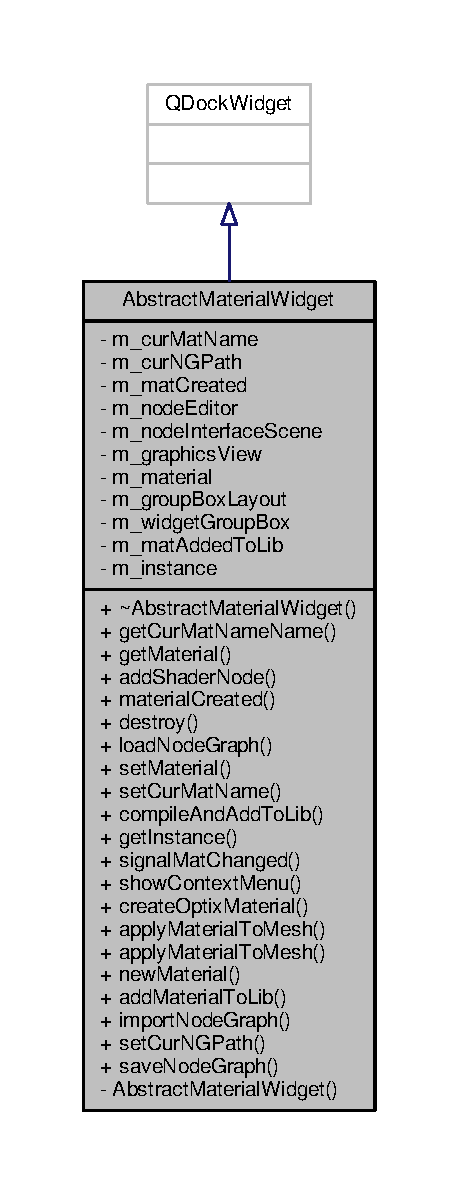
\includegraphics[height=550pt]{class_abstract_material_widget__inherit__graph}
\end{center}
\end{figure}


Collaboration diagram for Abstract\-Material\-Widget\-:
\nopagebreak
\begin{figure}[H]
\begin{center}
\leavevmode
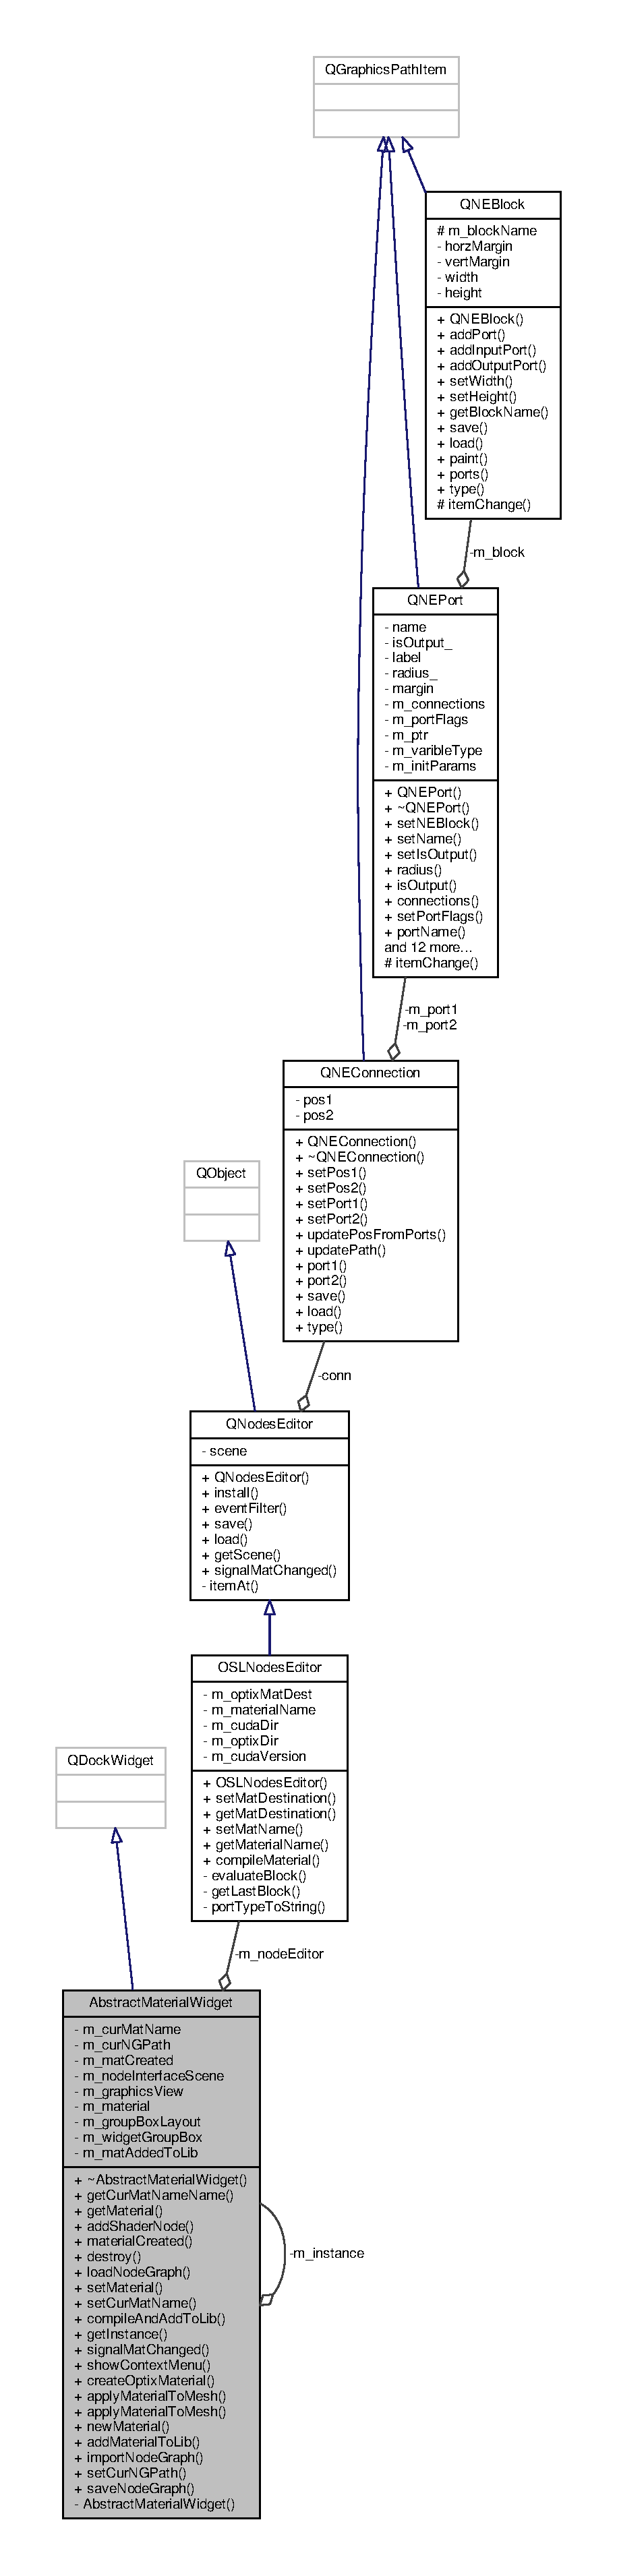
\includegraphics[height=550pt]{class_abstract_material_widget__coll__graph}
\end{center}
\end{figure}
\subsection*{Public Slots}
\begin{DoxyCompactItemize}
\item 
\hypertarget{class_abstract_material_widget_a1443013bf1f4b913b8d69d10eeaca186}{void \hyperlink{class_abstract_material_widget_a1443013bf1f4b913b8d69d10eeaca186}{signal\-Mat\-Changed} ()}\label{class_abstract_material_widget_a1443013bf1f4b913b8d69d10eeaca186}

\begin{DoxyCompactList}\small\item\em slot to be called to signal if the material has been changed \end{DoxyCompactList}\item 
\hypertarget{class_abstract_material_widget_a5ef500ae0f272d97fb4687ac0c6fd114}{void \hyperlink{class_abstract_material_widget_a5ef500ae0f272d97fb4687ac0c6fd114}{show\-Context\-Menu} (const Q\-Point \&pos)}\label{class_abstract_material_widget_a5ef500ae0f272d97fb4687ac0c6fd114}

\begin{DoxyCompactList}\small\item\em Create a slot to show our context menu if we right click anywhere on our widget. \end{DoxyCompactList}\item 
\hypertarget{class_abstract_material_widget_aae96067fbd8e7c2cdd686688bc25c3fd}{void \hyperlink{class_abstract_material_widget_aae96067fbd8e7c2cdd686688bc25c3fd}{create\-Optix\-Material} ()}\label{class_abstract_material_widget_aae96067fbd8e7c2cdd686688bc25c3fd}

\begin{DoxyCompactList}\small\item\em Slot to create a material from our O\-S\-L node graph. \end{DoxyCompactList}\item 
void \hyperlink{class_abstract_material_widget_a7085b0419e52157f46312928d9bfc326}{apply\-Material\-To\-Mesh} (std\-::string \-\_\-mesh)
\begin{DoxyCompactList}\small\item\em applies the current createed material to mesh of choosing \end{DoxyCompactList}\item 
\hypertarget{class_abstract_material_widget_a02cc4a4c8e489854363c646cd67c03f7}{void \hyperlink{class_abstract_material_widget_a02cc4a4c8e489854363c646cd67c03f7}{apply\-Material\-To\-Mesh} ()}\label{class_abstract_material_widget_a02cc4a4c8e489854363c646cd67c03f7}

\begin{DoxyCompactList}\small\item\em applies material to currently selected mesh \end{DoxyCompactList}\item 
\hypertarget{class_abstract_material_widget_ae3fc9533799259797b676f07d084211f}{void \hyperlink{class_abstract_material_widget_ae3fc9533799259797b676f07d084211f}{new\-Material} ()}\label{class_abstract_material_widget_ae3fc9533799259797b676f07d084211f}

\begin{DoxyCompactList}\small\item\em slot to create a new material \end{DoxyCompactList}\item 
\hypertarget{class_abstract_material_widget_ab4350dfde2aadd6e6c42210ec03a4dd1}{bool \hyperlink{class_abstract_material_widget_ab4350dfde2aadd6e6c42210ec03a4dd1}{add\-Material\-To\-Lib} ()}\label{class_abstract_material_widget_ab4350dfde2aadd6e6c42210ec03a4dd1}

\begin{DoxyCompactList}\small\item\em slot to add our material to our library \end{DoxyCompactList}\item 
\hypertarget{class_abstract_material_widget_ac4c17109d68c6540f5cfbcd3c409db3a}{void \hyperlink{class_abstract_material_widget_ac4c17109d68c6540f5cfbcd3c409db3a}{import\-Node\-Graph} ()}\label{class_abstract_material_widget_ac4c17109d68c6540f5cfbcd3c409db3a}

\begin{DoxyCompactList}\small\item\em slot to load node graphs to our scene \end{DoxyCompactList}\item 
void \hyperlink{class_abstract_material_widget_acf6a38c7f984df1eb5470780f1f8aa83}{set\-Cur\-N\-G\-Path} (Q\-String \-\_\-path)
\begin{DoxyCompactList}\small\item\em set the path to the current node graph file \end{DoxyCompactList}\item 
\hypertarget{class_abstract_material_widget_a314c224671ac3e3aa56d313eaa95398f}{void \hyperlink{class_abstract_material_widget_a314c224671ac3e3aa56d313eaa95398f}{save\-Node\-Graph} ()}\label{class_abstract_material_widget_a314c224671ac3e3aa56d313eaa95398f}

\begin{DoxyCompactList}\small\item\em saves our current node graph \end{DoxyCompactList}\end{DoxyCompactItemize}
\subsection*{Signals}
\begin{DoxyCompactItemize}
\item 
\hypertarget{class_abstract_material_widget_a57872e797feedc126fc15823c5b6d8e2}{void \hyperlink{class_abstract_material_widget_a57872e797feedc126fc15823c5b6d8e2}{mat\-Changed} ()}\label{class_abstract_material_widget_a57872e797feedc126fc15823c5b6d8e2}

\begin{DoxyCompactList}\small\item\em if the material has changed in some way \end{DoxyCompactList}\end{DoxyCompactItemize}
\subsection*{Public Member Functions}
\begin{DoxyCompactItemize}
\item 
\hypertarget{class_abstract_material_widget_af5dcc2f282ee2b607c7cfb132fd96b12}{\hyperlink{class_abstract_material_widget_af5dcc2f282ee2b607c7cfb132fd96b12}{$\sim$\-Abstract\-Material\-Widget} ()}\label{class_abstract_material_widget_af5dcc2f282ee2b607c7cfb132fd96b12}

\begin{DoxyCompactList}\small\item\em our default destructor. Deals with our gabage collection \end{DoxyCompactList}\item 
\hypertarget{class_abstract_material_widget_a3e25d0095c98840a1705fcb34a78441b}{std\-::string \hyperlink{class_abstract_material_widget_a3e25d0095c98840a1705fcb34a78441b}{get\-Cur\-Mat\-Name\-Name} ()}\label{class_abstract_material_widget_a3e25d0095c98840a1705fcb34a78441b}

\begin{DoxyCompactList}\small\item\em accessor to the name of our material \end{DoxyCompactList}\item 
\hypertarget{class_abstract_material_widget_a85987f671b7e4c284f6d7d39d834d800}{optix\-::\-Material \hyperlink{class_abstract_material_widget_a85987f671b7e4c284f6d7d39d834d800}{get\-Material} ()}\label{class_abstract_material_widget_a85987f671b7e4c284f6d7d39d834d800}

\begin{DoxyCompactList}\small\item\em accessot to our material \end{DoxyCompactList}\item 
\hypertarget{class_abstract_material_widget_a24133fd1d3a66d898ca30a69b8f9cff3}{void \hyperlink{class_abstract_material_widget_a24133fd1d3a66d898ca30a69b8f9cff3}{add\-Shader\-Node} ()}\label{class_abstract_material_widget_a24133fd1d3a66d898ca30a69b8f9cff3}

\begin{DoxyCompactList}\small\item\em adds a shader node to our user interface \end{DoxyCompactList}\item 
\hypertarget{class_abstract_material_widget_ac7b5ac03177e6f3779b055c2ae872308}{bool \hyperlink{class_abstract_material_widget_ac7b5ac03177e6f3779b055c2ae872308}{material\-Created} ()}\label{class_abstract_material_widget_ac7b5ac03177e6f3779b055c2ae872308}

\begin{DoxyCompactList}\small\item\em query if a material has been created \end{DoxyCompactList}\item 
\hypertarget{class_abstract_material_widget_a4c08ffa418405cfb09de9ce04716d21c}{void \hyperlink{class_abstract_material_widget_a4c08ffa418405cfb09de9ce04716d21c}{destroy} ()}\label{class_abstract_material_widget_a4c08ffa418405cfb09de9ce04716d21c}

\begin{DoxyCompactList}\small\item\em removes our singleton class from existence \end{DoxyCompactList}\item 
void \hyperlink{class_abstract_material_widget_ab697eed181925e2511b385b07ed13780}{load\-Node\-Graph} (Q\-String \-\_\-path)
\begin{DoxyCompactList}\small\item\em loads a nodegraph from a file \end{DoxyCompactList}\item 
\hypertarget{class_abstract_material_widget_a275ddde6f459273d70597e54896f0ba2}{void \hyperlink{class_abstract_material_widget_a275ddde6f459273d70597e54896f0ba2}{set\-Material} (optix\-::\-Material \-\_\-mat, bool \-\_\-in\-Library=false)}\label{class_abstract_material_widget_a275ddde6f459273d70597e54896f0ba2}

\begin{DoxyCompactList}\small\item\em mutator to our optix material \end{DoxyCompactList}\item 
\hypertarget{class_abstract_material_widget_aa5c700df91c81fae3ed650abb315ce43}{void \hyperlink{class_abstract_material_widget_aa5c700df91c81fae3ed650abb315ce43}{set\-Cur\-Mat\-Name} (std\-::string \-\_\-name)}\label{class_abstract_material_widget_aa5c700df91c81fae3ed650abb315ce43}

\begin{DoxyCompactList}\small\item\em set the current material name \end{DoxyCompactList}\item 
\hypertarget{class_abstract_material_widget_a965876cda41ec655a45c2c34d86a97ae}{void \hyperlink{class_abstract_material_widget_a965876cda41ec655a45c2c34d86a97ae}{compile\-And\-Add\-To\-Lib} (Q\-String \-\_\-path)}\label{class_abstract_material_widget_a965876cda41ec655a45c2c34d86a97ae}

\begin{DoxyCompactList}\small\item\em compiles destination file and adds to material library \end{DoxyCompactList}\end{DoxyCompactItemize}
\subsection*{Static Public Member Functions}
\begin{DoxyCompactItemize}
\item 
\hypertarget{class_abstract_material_widget_a96533d07fe6cc79527f5df9ddf2199a7}{static \hyperlink{class_abstract_material_widget}{Abstract\-Material\-Widget} $\ast$ \hyperlink{class_abstract_material_widget_a96533d07fe6cc79527f5df9ddf2199a7}{get\-Instance} (Q\-Widget $\ast$parent=0)}\label{class_abstract_material_widget_a96533d07fe6cc79527f5df9ddf2199a7}

\begin{DoxyCompactList}\small\item\em accessor to our instance of our class \end{DoxyCompactList}\end{DoxyCompactItemize}
\subsection*{Private Member Functions}
\begin{DoxyCompactItemize}
\item 
\hypertarget{class_abstract_material_widget_ace749c971293b2aef90e2861500be8bd}{\hyperlink{class_abstract_material_widget_ace749c971293b2aef90e2861500be8bd}{Abstract\-Material\-Widget} (Q\-Widget $\ast$parent=0)}\label{class_abstract_material_widget_ace749c971293b2aef90e2861500be8bd}

\begin{DoxyCompactList}\small\item\em our default constructor \end{DoxyCompactList}\end{DoxyCompactItemize}
\subsection*{Private Attributes}
\begin{DoxyCompactItemize}
\item 
\hypertarget{class_abstract_material_widget_aa24e234565e46730e0102263774a380c}{std\-::string \hyperlink{class_abstract_material_widget_aa24e234565e46730e0102263774a380c}{m\-\_\-cur\-Mat\-Name}}\label{class_abstract_material_widget_aa24e234565e46730e0102263774a380c}

\begin{DoxyCompactList}\small\item\em the current material name \end{DoxyCompactList}\item 
\hypertarget{class_abstract_material_widget_a5cd78b14d7ada8dcb73cbd9c03f6d2a9}{Q\-String \hyperlink{class_abstract_material_widget_a5cd78b14d7ada8dcb73cbd9c03f6d2a9}{m\-\_\-cur\-N\-G\-Path}}\label{class_abstract_material_widget_a5cd78b14d7ada8dcb73cbd9c03f6d2a9}

\begin{DoxyCompactList}\small\item\em Path to our current node graph. \end{DoxyCompactList}\item 
\hypertarget{class_abstract_material_widget_ae03c748d938aa021c7f18d2a064895f4}{bool \hyperlink{class_abstract_material_widget_ae03c748d938aa021c7f18d2a064895f4}{m\-\_\-mat\-Created}}\label{class_abstract_material_widget_ae03c748d938aa021c7f18d2a064895f4}

\begin{DoxyCompactList}\small\item\em a bool to indicate if a material has been successfuly created \end{DoxyCompactList}\item 
\hypertarget{class_abstract_material_widget_aa0cfa5f820744336c4d75d957576998b}{\hyperlink{class_o_s_l_nodes_editor}{O\-S\-L\-Nodes\-Editor} $\ast$ \hyperlink{class_abstract_material_widget_aa0cfa5f820744336c4d75d957576998b}{m\-\_\-node\-Editor}}\label{class_abstract_material_widget_aa0cfa5f820744336c4d75d957576998b}

\begin{DoxyCompactList}\small\item\em Q\-Node\-Editor that manges loading and saving of our node graph. \end{DoxyCompactList}\item 
\hypertarget{class_abstract_material_widget_a96104151aec95df4b3eecf56486c5cfc}{Q\-Graphics\-Scene $\ast$ \hyperlink{class_abstract_material_widget_a96104151aec95df4b3eecf56486c5cfc}{m\-\_\-node\-Interface\-Scene}}\label{class_abstract_material_widget_a96104151aec95df4b3eecf56486c5cfc}

\begin{DoxyCompactList}\small\item\em Q\-Graphics scene which will hold the node interface. \end{DoxyCompactList}\item 
\hypertarget{class_abstract_material_widget_a9e3d797b92f1518223ff4f48d1c35918}{Q\-Graphics\-View $\ast$ \hyperlink{class_abstract_material_widget_a9e3d797b92f1518223ff4f48d1c35918}{m\-\_\-graphics\-View}}\label{class_abstract_material_widget_a9e3d797b92f1518223ff4f48d1c35918}

\begin{DoxyCompactList}\small\item\em Q\-Graphics\-View which will hold our material graph scene. \end{DoxyCompactList}\item 
\hypertarget{class_abstract_material_widget_afd84a89a0bfff011f67af8b844a156c9}{optix\-::\-Material \hyperlink{class_abstract_material_widget_afd84a89a0bfff011f67af8b844a156c9}{m\-\_\-material}}\label{class_abstract_material_widget_afd84a89a0bfff011f67af8b844a156c9}

\begin{DoxyCompactList}\small\item\em Our optix material. \end{DoxyCompactList}\item 
\hypertarget{class_abstract_material_widget_aabf9f661c778f9f2926777f5177ed176}{Q\-Grid\-Layout $\ast$ \hyperlink{class_abstract_material_widget_aabf9f661c778f9f2926777f5177ed176}{m\-\_\-group\-Box\-Layout}}\label{class_abstract_material_widget_aabf9f661c778f9f2926777f5177ed176}

\begin{DoxyCompactList}\small\item\em the layout of our group box \end{DoxyCompactList}\item 
\hypertarget{class_abstract_material_widget_a2267d86e075a49f0b127a0dc53f4a924}{Q\-Group\-Box $\ast$ \hyperlink{class_abstract_material_widget_a2267d86e075a49f0b127a0dc53f4a924}{m\-\_\-widget\-Group\-Box}}\label{class_abstract_material_widget_a2267d86e075a49f0b127a0dc53f4a924}

\begin{DoxyCompactList}\small\item\em a group box to hold all our widgets buttons \end{DoxyCompactList}\item 
\hypertarget{class_abstract_material_widget_abf17d1069b4ed91bc0fccbf724404ef9}{bool \hyperlink{class_abstract_material_widget_abf17d1069b4ed91bc0fccbf724404ef9}{m\-\_\-mat\-Added\-To\-Lib}}\label{class_abstract_material_widget_abf17d1069b4ed91bc0fccbf724404ef9}

\begin{DoxyCompactList}\small\item\em bool to indicate if our material has been added to our library already \end{DoxyCompactList}\end{DoxyCompactItemize}
\subsection*{Static Private Attributes}
\begin{DoxyCompactItemize}
\item 
\hypertarget{class_abstract_material_widget_a73496d58f2f8e06da9fdac08f9757dfa}{static \hyperlink{class_abstract_material_widget}{Abstract\-Material\-Widget} $\ast$ \hyperlink{class_abstract_material_widget_a73496d58f2f8e06da9fdac08f9757dfa}{m\-\_\-instance}}\label{class_abstract_material_widget_a73496d58f2f8e06da9fdac08f9757dfa}

\begin{DoxyCompactList}\small\item\em our instance of our node graph widget \end{DoxyCompactList}\end{DoxyCompactItemize}


\subsection{Detailed Description}
an abstract material widget that creates a simple setup 

\begin{DoxyAuthor}{Author}
Declan Russell 
\end{DoxyAuthor}
\begin{DoxyDate}{Date}
05/03/15 so that we can quickly create a U\-I for an optix material. 
\end{DoxyDate}


\subsection{Member Function Documentation}
\hypertarget{class_abstract_material_widget_a7085b0419e52157f46312928d9bfc326}{\index{Abstract\-Material\-Widget@{Abstract\-Material\-Widget}!apply\-Material\-To\-Mesh@{apply\-Material\-To\-Mesh}}
\index{apply\-Material\-To\-Mesh@{apply\-Material\-To\-Mesh}!AbstractMaterialWidget@{Abstract\-Material\-Widget}}
\subsubsection[{apply\-Material\-To\-Mesh}]{\setlength{\rightskip}{0pt plus 5cm}void Abstract\-Material\-Widget\-::apply\-Material\-To\-Mesh (
\begin{DoxyParamCaption}
\item[{std\-::string}]{\-\_\-mesh}
\end{DoxyParamCaption}
)\hspace{0.3cm}{\ttfamily [slot]}}}\label{class_abstract_material_widget_a7085b0419e52157f46312928d9bfc326}


applies the current createed material to mesh of choosing 


\begin{DoxyParams}{Parameters}
{\em \-\_\-mesh} & -\/ the mesh name to apply the material to \\
\hline
\end{DoxyParams}


Here is the call graph for this function\-:
\nopagebreak
\begin{figure}[H]
\begin{center}
\leavevmode
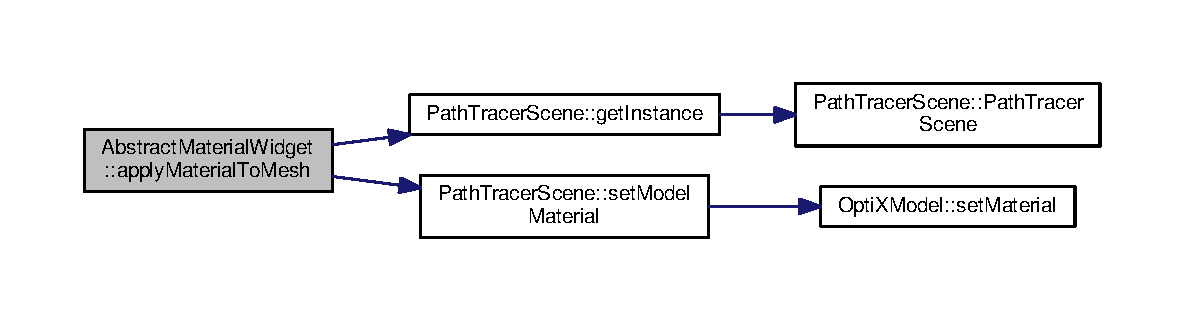
\includegraphics[width=350pt]{class_abstract_material_widget_a7085b0419e52157f46312928d9bfc326_cgraph}
\end{center}
\end{figure}


\hypertarget{class_abstract_material_widget_ab697eed181925e2511b385b07ed13780}{\index{Abstract\-Material\-Widget@{Abstract\-Material\-Widget}!load\-Node\-Graph@{load\-Node\-Graph}}
\index{load\-Node\-Graph@{load\-Node\-Graph}!AbstractMaterialWidget@{Abstract\-Material\-Widget}}
\subsubsection[{load\-Node\-Graph}]{\setlength{\rightskip}{0pt plus 5cm}void Abstract\-Material\-Widget\-::load\-Node\-Graph (
\begin{DoxyParamCaption}
\item[{Q\-String}]{\-\_\-path}
\end{DoxyParamCaption}
)}}\label{class_abstract_material_widget_ab697eed181925e2511b385b07ed13780}


loads a nodegraph from a file 


\begin{DoxyParams}{Parameters}
{\em \-\_\-path} & -\/ path to node graph \\
\hline
\end{DoxyParams}


Here is the caller graph for this function\-:
\nopagebreak
\begin{figure}[H]
\begin{center}
\leavevmode
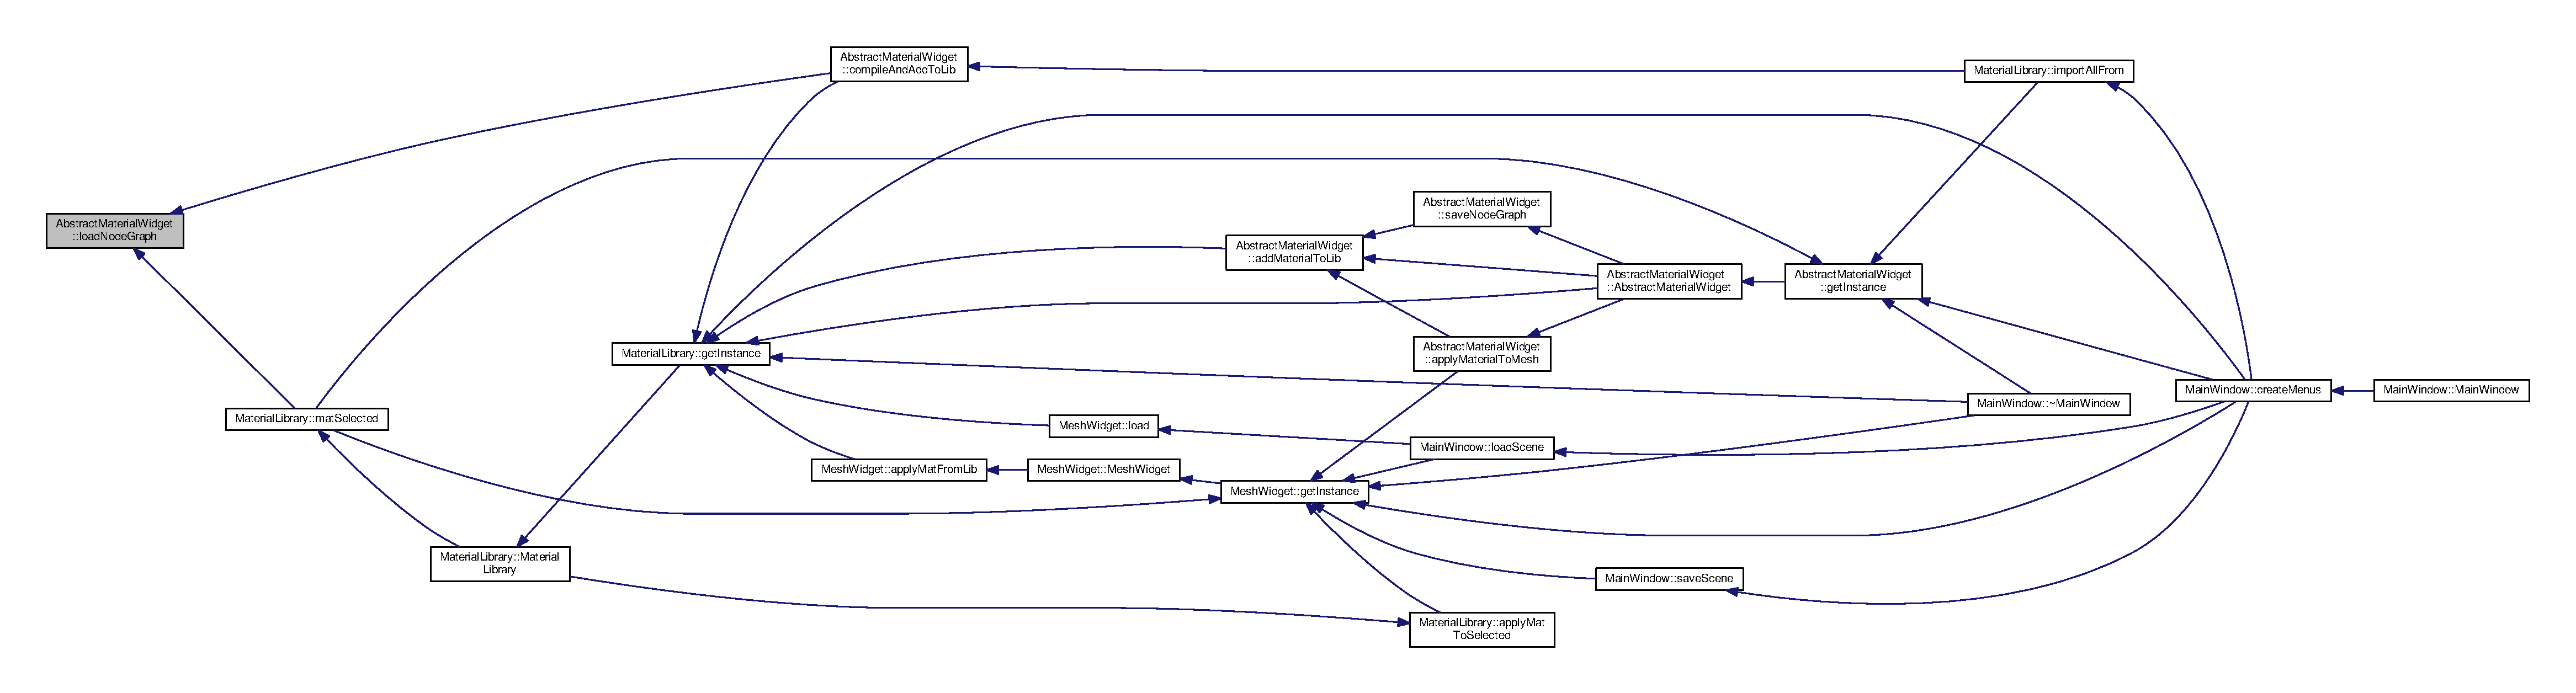
\includegraphics[width=350pt]{class_abstract_material_widget_ab697eed181925e2511b385b07ed13780_icgraph}
\end{center}
\end{figure}


\hypertarget{class_abstract_material_widget_acf6a38c7f984df1eb5470780f1f8aa83}{\index{Abstract\-Material\-Widget@{Abstract\-Material\-Widget}!set\-Cur\-N\-G\-Path@{set\-Cur\-N\-G\-Path}}
\index{set\-Cur\-N\-G\-Path@{set\-Cur\-N\-G\-Path}!AbstractMaterialWidget@{Abstract\-Material\-Widget}}
\subsubsection[{set\-Cur\-N\-G\-Path}]{\setlength{\rightskip}{0pt plus 5cm}void Abstract\-Material\-Widget\-::set\-Cur\-N\-G\-Path (
\begin{DoxyParamCaption}
\item[{Q\-String}]{\-\_\-path}
\end{DoxyParamCaption}
)\hspace{0.3cm}{\ttfamily [inline]}, {\ttfamily [slot]}}}\label{class_abstract_material_widget_acf6a38c7f984df1eb5470780f1f8aa83}


set the path to the current node graph file 


\begin{DoxyParams}{Parameters}
{\em \-\_\-path} & -\/ path to nodegraph \\
\hline
\end{DoxyParams}


The documentation for this class was generated from the following files\-:\begin{DoxyCompactItemize}
\item 
include/\-U\-I/Abstract\-Material\-Widget.\-h\item 
moc/moc\-\_\-\-Abstract\-Material\-Widget.\-cpp\item 
src/\-U\-I/Abstract\-Material\-Widget.\-cpp\end{DoxyCompactItemize}

\hypertarget{class_abstract_node_proxy_widget}{\section{Abstract\-Node\-Proxy\-Widget Class Reference}
\label{class_abstract_node_proxy_widget}\index{Abstract\-Node\-Proxy\-Widget@{Abstract\-Node\-Proxy\-Widget}}
}


Abstract base class for all variable proxy widgets in our scene.  




{\ttfamily \#include $<$Abstract\-Node\-Proxy\-Widget.\-h$>$}



Inheritance diagram for Abstract\-Node\-Proxy\-Widget\-:
\nopagebreak
\begin{figure}[H]
\begin{center}
\leavevmode
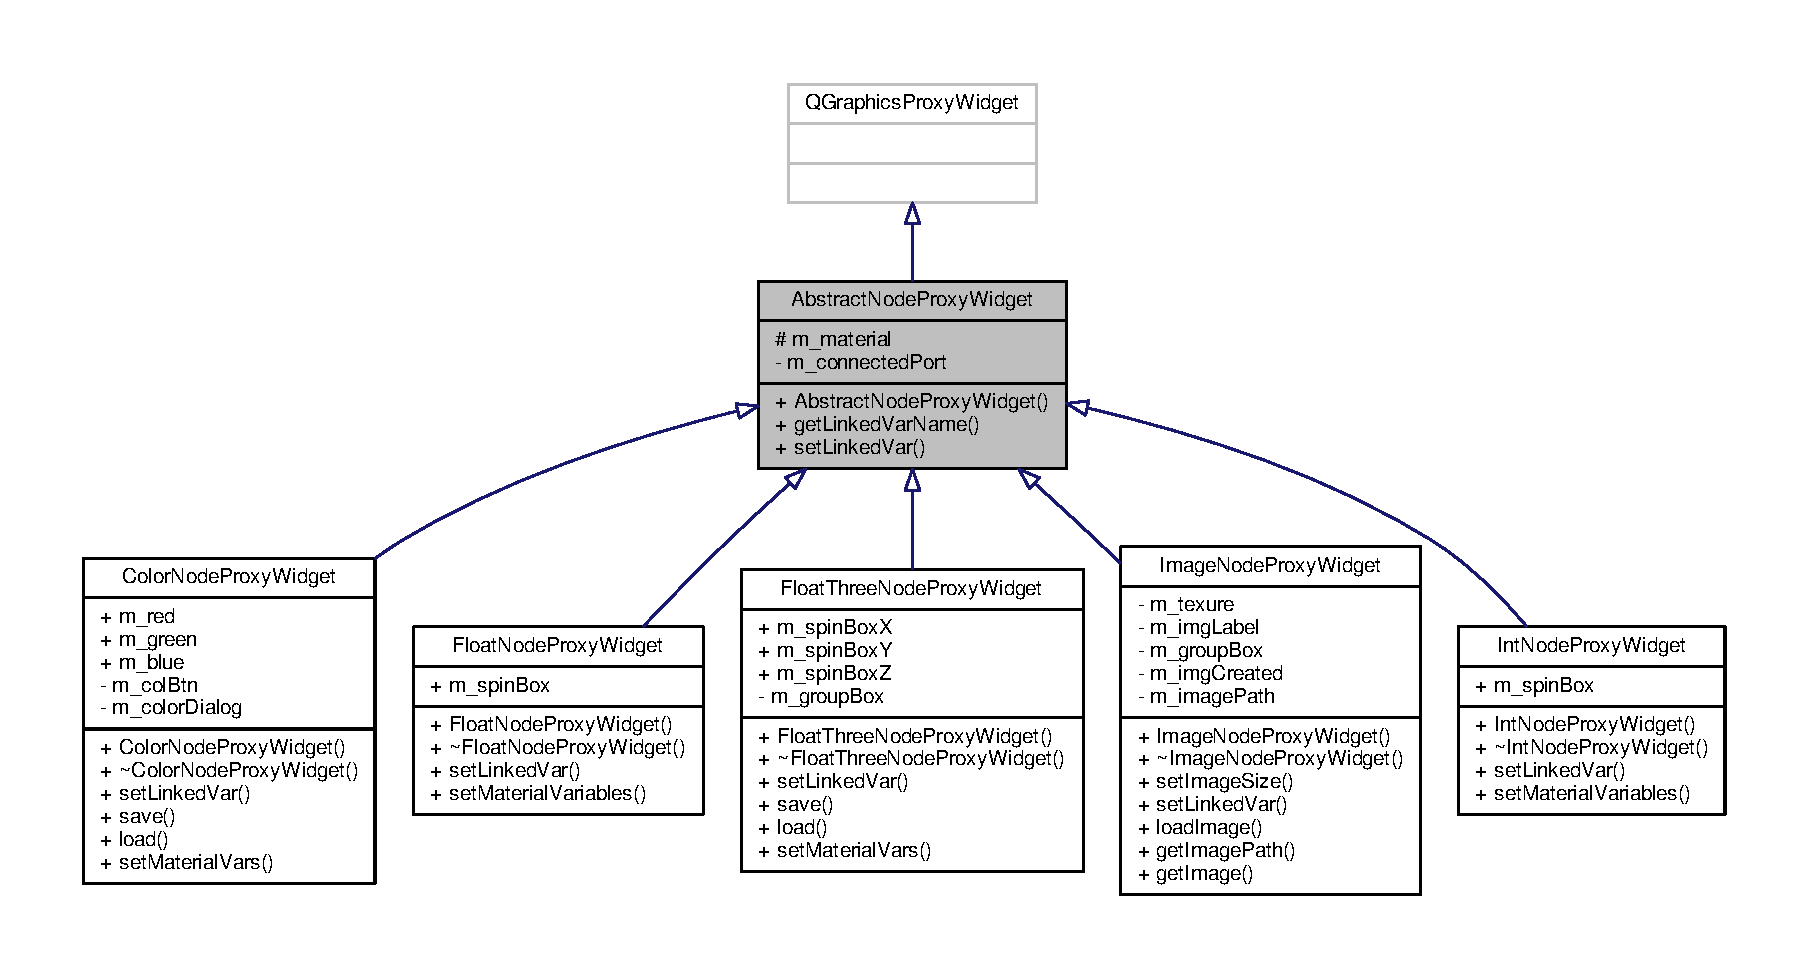
\includegraphics[width=350pt]{class_abstract_node_proxy_widget__inherit__graph}
\end{center}
\end{figure}


Collaboration diagram for Abstract\-Node\-Proxy\-Widget\-:
\nopagebreak
\begin{figure}[H]
\begin{center}
\leavevmode
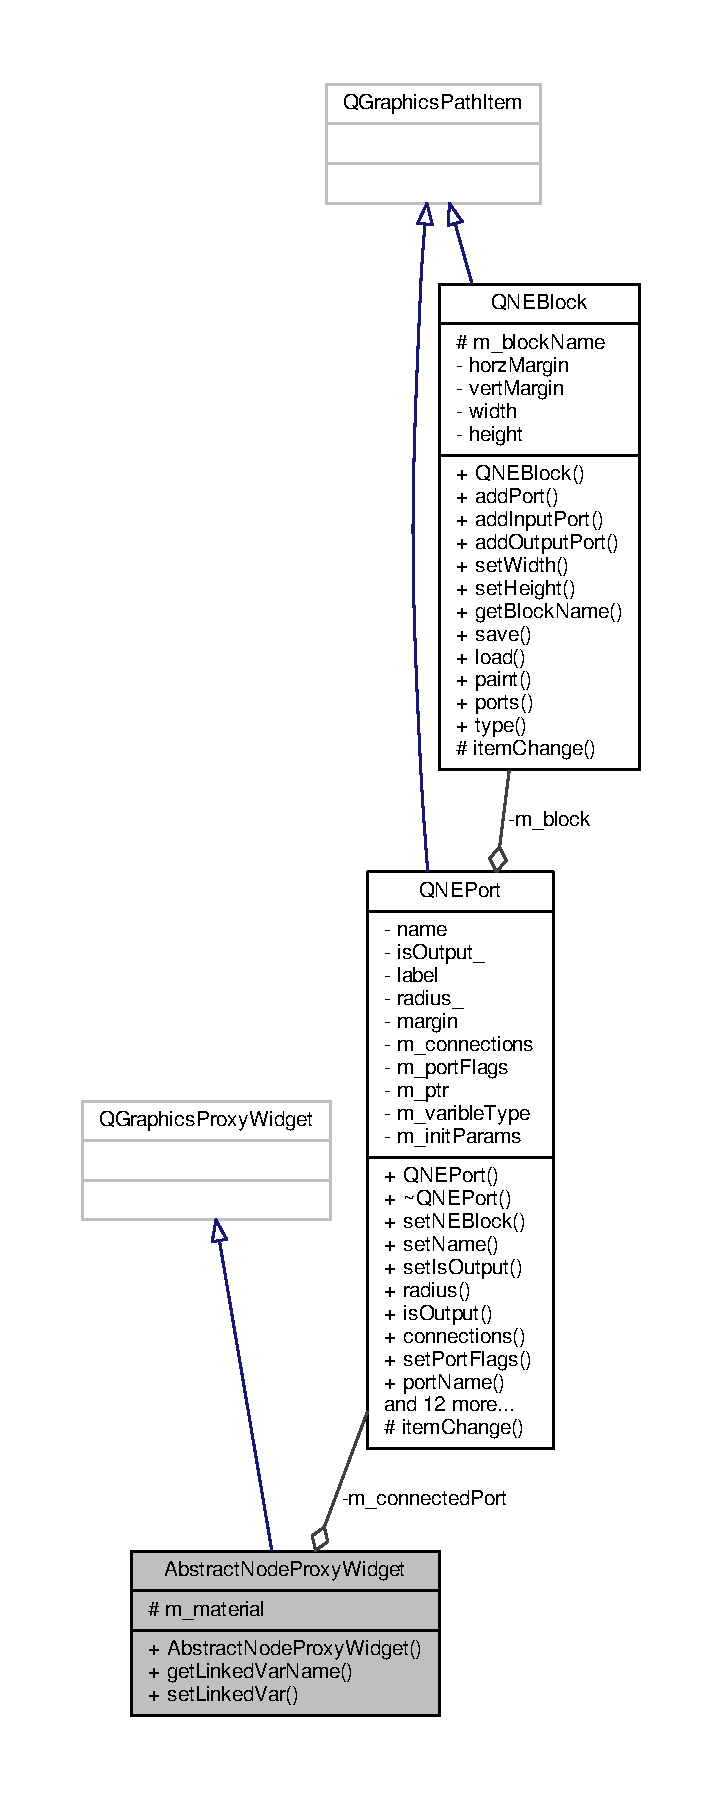
\includegraphics[height=550pt]{class_abstract_node_proxy_widget__coll__graph}
\end{center}
\end{figure}
\subsection*{Signals}
\begin{DoxyCompactItemize}
\item 
\hypertarget{class_abstract_node_proxy_widget_a503fe31eb1e4ff86ee211c18bb11a46e}{void \hyperlink{class_abstract_node_proxy_widget_a503fe31eb1e4ff86ee211c18bb11a46e}{attribute\-Changed} ()}\label{class_abstract_node_proxy_widget_a503fe31eb1e4ff86ee211c18bb11a46e}

\begin{DoxyCompactList}\small\item\em signal to notify if an attribute has changed \end{DoxyCompactList}\end{DoxyCompactItemize}
\subsection*{Public Member Functions}
\begin{DoxyCompactItemize}
\item 
\hypertarget{class_abstract_node_proxy_widget_a7ffe16a97b194e29c4bc15983e85402f}{\hyperlink{class_abstract_node_proxy_widget_a7ffe16a97b194e29c4bc15983e85402f}{Abstract\-Node\-Proxy\-Widget} (\hyperlink{class_q_n_e_port}{Q\-N\-E\-Port} $\ast$\-\_\-connected\-Port, optix\-::\-Material \&\-\_\-mat, Q\-Graphics\-Item $\ast$\-\_\-parent=0)}\label{class_abstract_node_proxy_widget_a7ffe16a97b194e29c4bc15983e85402f}

\begin{DoxyCompactList}\small\item\em our default constructor \end{DoxyCompactList}\item 
void \hyperlink{class_abstract_node_proxy_widget_aeac0d3fa1930be2396e2ab7c5bf04d35}{get\-Linked\-Var\-Name} (std\-::vector$<$ std\-::string $>$ \&\-\_\-linked\-Var\-Names)
\begin{DoxyCompactList}\small\item\em returns the linked varible name connected to desired port \end{DoxyCompactList}\item 
\hypertarget{class_abstract_node_proxy_widget_a0ffa73887a7646a6aaec547c81231617}{virtual void \hyperlink{class_abstract_node_proxy_widget_a0ffa73887a7646a6aaec547c81231617}{set\-Linked\-Var} ()}\label{class_abstract_node_proxy_widget_a0ffa73887a7646a6aaec547c81231617}

\begin{DoxyCompactList}\small\item\em virtual method to set whatever linked variables we have \end{DoxyCompactList}\end{DoxyCompactItemize}
\subsection*{Protected Attributes}
\begin{DoxyCompactItemize}
\item 
\hypertarget{class_abstract_node_proxy_widget_a141801dfcb39ad2b60f61b7a98e95ea5}{optix\-::\-Material \hyperlink{class_abstract_node_proxy_widget_a141801dfcb39ad2b60f61b7a98e95ea5}{m\-\_\-material}}\label{class_abstract_node_proxy_widget_a141801dfcb39ad2b60f61b7a98e95ea5}

\begin{DoxyCompactList}\small\item\em a member to hold the material to be edited \end{DoxyCompactList}\end{DoxyCompactItemize}
\subsection*{Private Attributes}
\begin{DoxyCompactItemize}
\item 
\hypertarget{class_abstract_node_proxy_widget_a0aaa8236fc7633a79b32576024c22434}{\hyperlink{class_q_n_e_port}{Q\-N\-E\-Port} $\ast$ \hyperlink{class_abstract_node_proxy_widget_a0aaa8236fc7633a79b32576024c22434}{m\-\_\-connected\-Port}}\label{class_abstract_node_proxy_widget_a0aaa8236fc7633a79b32576024c22434}

\begin{DoxyCompactList}\small\item\em a pointer to the port linked to our spin box \end{DoxyCompactList}\end{DoxyCompactItemize}


\subsection{Detailed Description}
Abstract base class for all variable proxy widgets in our scene. 

This extends from Q\-Graphics\-Proxy\-Widget which allows us to attach Q\-Widgets onto Q\-Graphics\-Items. We need this got the ability to user signals and slots to change attributes in our optix material \begin{DoxyAuthor}{Author}
Declan Russell 
\end{DoxyAuthor}
\begin{DoxyDate}{Date}
05/05/2015 
\end{DoxyDate}


\subsection{Member Function Documentation}
\hypertarget{class_abstract_node_proxy_widget_aeac0d3fa1930be2396e2ab7c5bf04d35}{\index{Abstract\-Node\-Proxy\-Widget@{Abstract\-Node\-Proxy\-Widget}!get\-Linked\-Var\-Name@{get\-Linked\-Var\-Name}}
\index{get\-Linked\-Var\-Name@{get\-Linked\-Var\-Name}!AbstractNodeProxyWidget@{Abstract\-Node\-Proxy\-Widget}}
\subsubsection[{get\-Linked\-Var\-Name}]{\setlength{\rightskip}{0pt plus 5cm}void Abstract\-Node\-Proxy\-Widget\-::get\-Linked\-Var\-Name (
\begin{DoxyParamCaption}
\item[{std\-::vector$<$ std\-::string $>$ \&}]{\-\_\-linked\-Var\-Names}
\end{DoxyParamCaption}
)}}\label{class_abstract_node_proxy_widget_aeac0d3fa1930be2396e2ab7c5bf04d35}


returns the linked varible name connected to desired port 


\begin{DoxyParams}{Parameters}
{\em \-\_\-linked\-Var\-Names} & -\/ vector of strings to store linked variable names \\
\hline
\end{DoxyParams}


Here is the call graph for this function\-:
\nopagebreak
\begin{figure}[H]
\begin{center}
\leavevmode
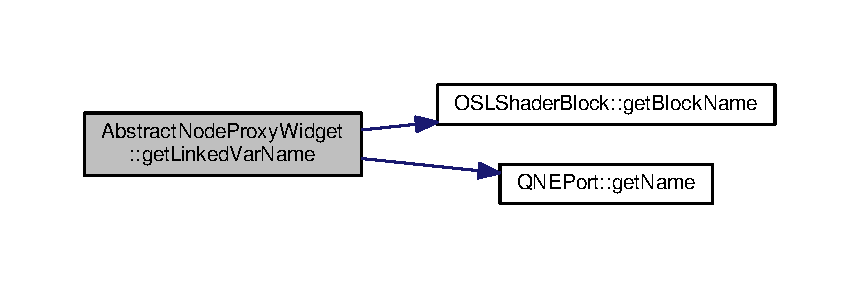
\includegraphics[width=350pt]{class_abstract_node_proxy_widget_aeac0d3fa1930be2396e2ab7c5bf04d35_cgraph}
\end{center}
\end{figure}




Here is the caller graph for this function\-:
\nopagebreak
\begin{figure}[H]
\begin{center}
\leavevmode
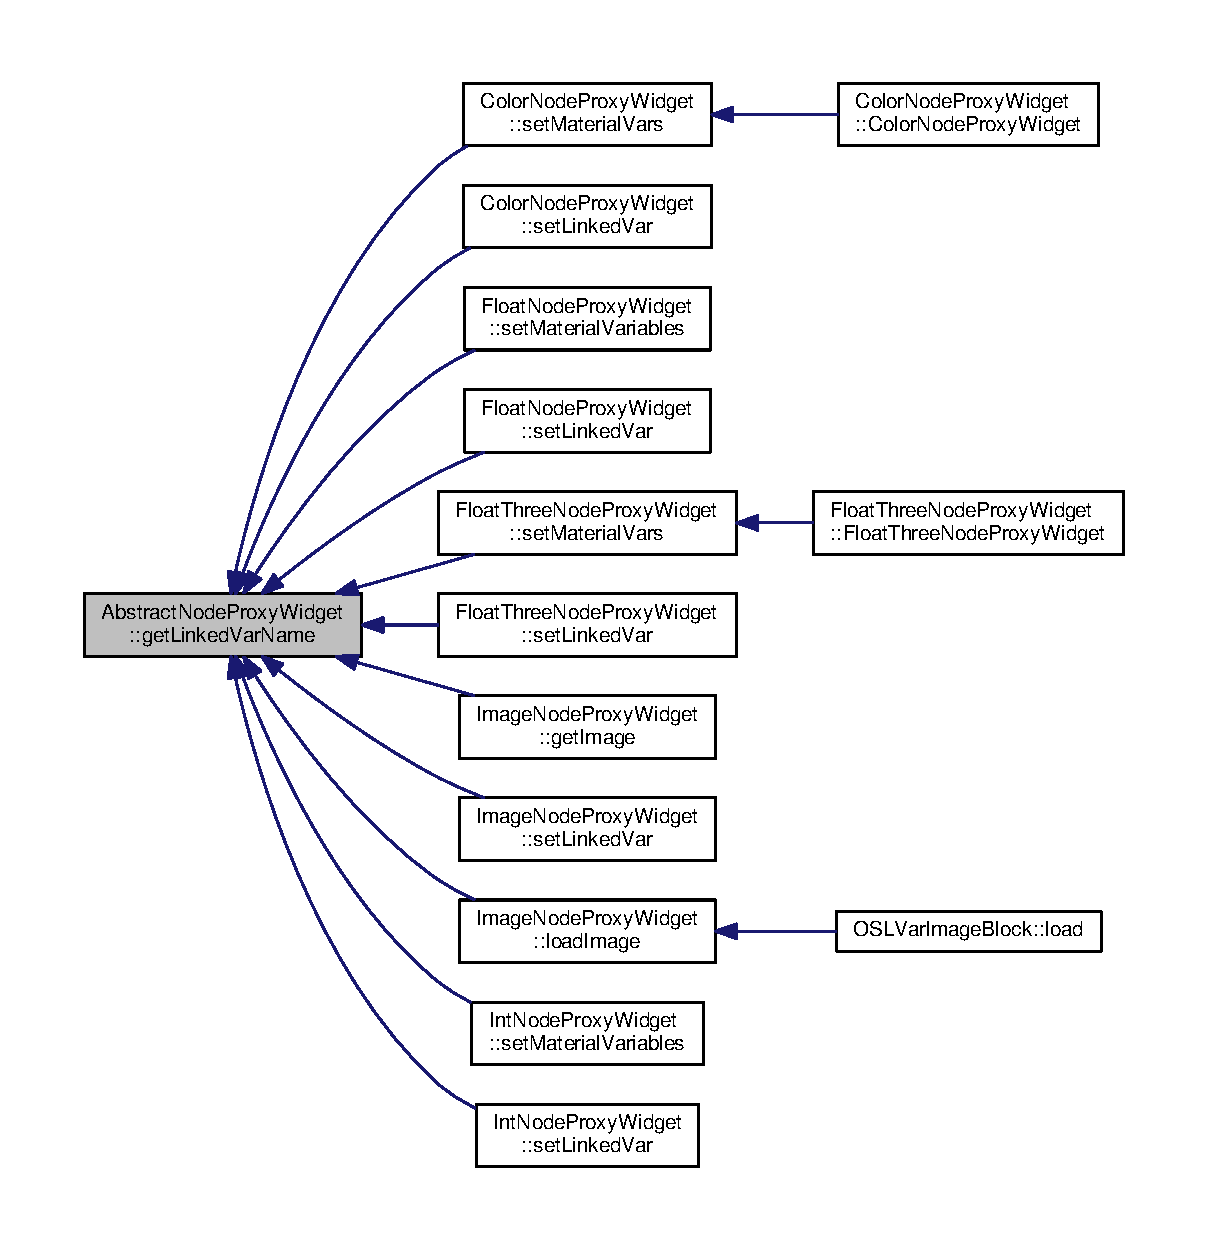
\includegraphics[width=350pt]{class_abstract_node_proxy_widget_aeac0d3fa1930be2396e2ab7c5bf04d35_icgraph}
\end{center}
\end{figure}




The documentation for this class was generated from the following files\-:\begin{DoxyCompactItemize}
\item 
include/\-Node\-Graph/Abstract\-Node\-Proxy\-Widget.\-h\item 
moc/moc\-\_\-\-Abstract\-Node\-Proxy\-Widget.\-cpp\item 
src/\-Node\-Graph/Abstract\-Node\-Proxy\-Widget.\-cpp\end{DoxyCompactItemize}

\hypertarget{class_camera}{\section{Camera Class Reference}
\label{class_camera}\index{Camera@{Camera}}
}


Collaboration diagram for Camera\-:
\nopagebreak
\begin{figure}[H]
\begin{center}
\leavevmode
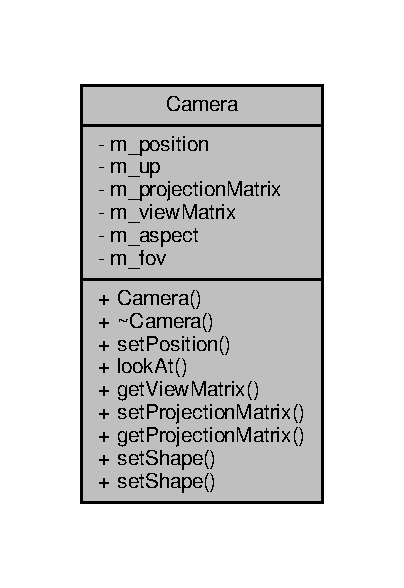
\includegraphics[width=194pt]{class_camera__coll__graph}
\end{center}
\end{figure}
\subsection*{Public Member Functions}
\begin{DoxyCompactItemize}
\item 
\hypertarget{class_camera_a583c769d57c096097a4cd55b0508acb9}{{\bfseries Camera} (glm\-::vec3 \-\_\-pos)}\label{class_camera_a583c769d57c096097a4cd55b0508acb9}

\item 
\hypertarget{class_camera_a4cfdd84e228c1353ee42ddd67059119b}{void {\bfseries set\-Position} (glm\-::vec3 \-\_\-position)}\label{class_camera_a4cfdd84e228c1353ee42ddd67059119b}

\item 
\hypertarget{class_camera_a0b021889f36bc9ba71eb55eef4d81651}{void {\bfseries look\-At} (glm\-::vec3 \-\_\-position, glm\-::vec3 \-\_\-center, glm\-::vec3 \-\_\-up)}\label{class_camera_a0b021889f36bc9ba71eb55eef4d81651}

\item 
\hypertarget{class_camera_a5569ca5967e01d3344fbf6aba36d9820}{glm\-::mat4 {\bfseries get\-View\-Matrix} ()}\label{class_camera_a5569ca5967e01d3344fbf6aba36d9820}

\item 
\hypertarget{class_camera_a2cb6fc559062f2c3aea4856d8838adf9}{void {\bfseries set\-Projection\-Matrix} (float \-\_\-fov, float \-\_\-aspect, float \-\_\-near, float \-\_\-far)}\label{class_camera_a2cb6fc559062f2c3aea4856d8838adf9}

\item 
\hypertarget{class_camera_adf09522521723786b9f405c99d6594c7}{glm\-::mat4 {\bfseries get\-Projection\-Matrix} ()}\label{class_camera_adf09522521723786b9f405c99d6594c7}

\item 
\hypertarget{class_camera_a019c5a2e4e223af12e8c1b6c48cd825b}{void {\bfseries set\-Shape} (float \-\_\-aspect)}\label{class_camera_a019c5a2e4e223af12e8c1b6c48cd825b}

\item 
\hypertarget{class_camera_ad279e684b491faecf277fb780e4b370f}{void {\bfseries set\-Shape} (float \-\_\-w, float \-\_\-h)}\label{class_camera_ad279e684b491faecf277fb780e4b370f}

\end{DoxyCompactItemize}
\subsection*{Private Attributes}
\begin{DoxyCompactItemize}
\item 
\hypertarget{class_camera_aa4d06d49524248f81823444fa2544da0}{glm\-::vec3 {\bfseries m\-\_\-position}}\label{class_camera_aa4d06d49524248f81823444fa2544da0}

\item 
\hypertarget{class_camera_af2a8632b36b3c7b1a79234ab4ccf4059}{glm\-::vec3 {\bfseries m\-\_\-up}}\label{class_camera_af2a8632b36b3c7b1a79234ab4ccf4059}

\item 
\hypertarget{class_camera_a26d7567bf34d14260f887a0382aeae29}{glm\-::mat4 {\bfseries m\-\_\-projection\-Matrix}}\label{class_camera_a26d7567bf34d14260f887a0382aeae29}

\item 
\hypertarget{class_camera_a11c9caa79662eca069eda13481913a25}{glm\-::mat4 {\bfseries m\-\_\-view\-Matrix}}\label{class_camera_a11c9caa79662eca069eda13481913a25}

\item 
\hypertarget{class_camera_abf58e1558e08e785c929f41b25615c30}{float {\bfseries m\-\_\-aspect}}\label{class_camera_abf58e1558e08e785c929f41b25615c30}

\item 
\hypertarget{class_camera_aa404a4e057fa16fb82ce8668d7a661b6}{float {\bfseries m\-\_\-fov}}\label{class_camera_aa404a4e057fa16fb82ce8668d7a661b6}

\end{DoxyCompactItemize}


The documentation for this class was generated from the following files\-:\begin{DoxyCompactItemize}
\item 
include/\-Core/Camera.\-h\item 
src/\-Core/Camera.\-cpp\end{DoxyCompactItemize}

\hypertarget{class_camera_widget}{\section{Camera\-Widget Class Reference}
\label{class_camera_widget}\index{Camera\-Widget@{Camera\-Widget}}
}


Inheritance diagram for Camera\-Widget\-:
\nopagebreak
\begin{figure}[H]
\begin{center}
\leavevmode
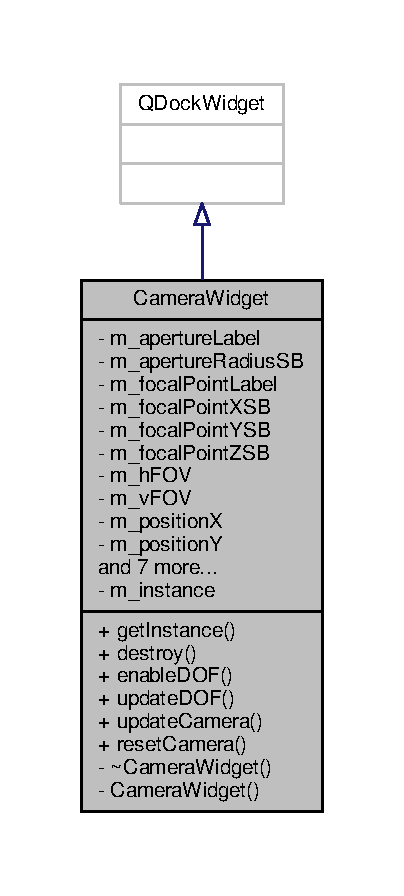
\includegraphics[width=194pt]{class_camera_widget__inherit__graph}
\end{center}
\end{figure}


Collaboration diagram for Camera\-Widget\-:
\nopagebreak
\begin{figure}[H]
\begin{center}
\leavevmode
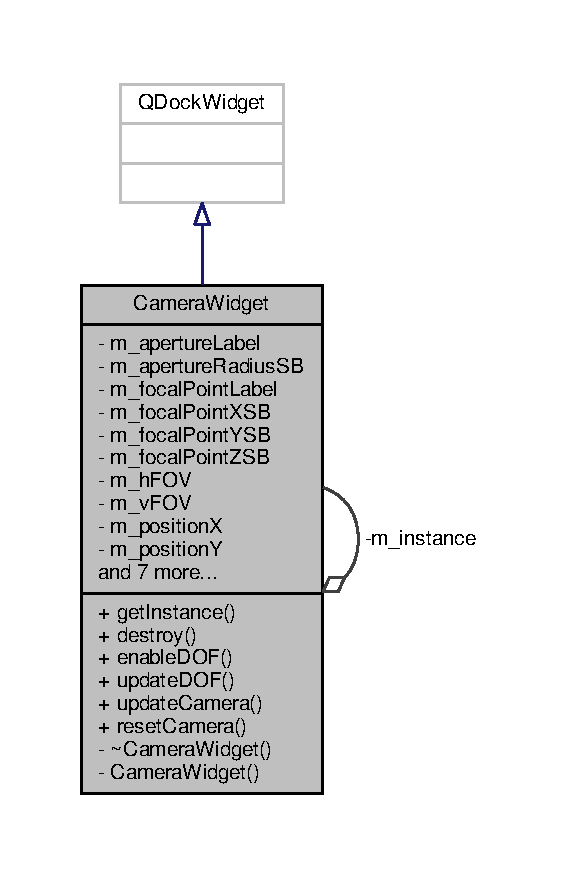
\includegraphics[width=270pt]{class_camera_widget__coll__graph}
\end{center}
\end{figure}
\subsection*{Public Slots}
\begin{DoxyCompactItemize}
\item 
\hypertarget{class_camera_widget_a61afcd6f680d6ec43b9949c6f324c047}{void \hyperlink{class_camera_widget_a61afcd6f680d6ec43b9949c6f324c047}{enable\-D\-O\-F} (bool \-\_\-enabled)}\label{class_camera_widget_a61afcd6f680d6ec43b9949c6f324c047}

\begin{DoxyCompactList}\small\item\em Enables the depth of field controls. \end{DoxyCompactList}\item 
\hypertarget{class_camera_widget_a94acbc0fd82c07bb2f77c09dc8aafd84}{void \hyperlink{class_camera_widget_a94acbc0fd82c07bb2f77c09dc8aafd84}{update\-D\-O\-F} ()}\label{class_camera_widget_a94acbc0fd82c07bb2f77c09dc8aafd84}

\begin{DoxyCompactList}\small\item\em Update D\-O\-F camera settings. \end{DoxyCompactList}\item 
\hypertarget{class_camera_widget_aafcf078d596c85bd61031163f855e3fa}{void \hyperlink{class_camera_widget_aafcf078d596c85bd61031163f855e3fa}{update\-Camera} ()}\label{class_camera_widget_aafcf078d596c85bd61031163f855e3fa}

\begin{DoxyCompactList}\small\item\em Update other camera settings. \end{DoxyCompactList}\item 
\hypertarget{class_camera_widget_a708a4a1499b94ed542268cd1de8fcb6e}{void \hyperlink{class_camera_widget_a708a4a1499b94ed542268cd1de8fcb6e}{reset\-Camera} ()}\label{class_camera_widget_a708a4a1499b94ed542268cd1de8fcb6e}

\begin{DoxyCompactList}\small\item\em Resets the camera. \end{DoxyCompactList}\end{DoxyCompactItemize}
\subsection*{Signals}
\begin{DoxyCompactItemize}
\item 
\hypertarget{class_camera_widget_a2d52203c831cd5bc904013def64f5e8e}{void \hyperlink{class_camera_widget_a2d52203c831cd5bc904013def64f5e8e}{update\-Scene} ()}\label{class_camera_widget_a2d52203c831cd5bc904013def64f5e8e}

\begin{DoxyCompactList}\small\item\em Update other camera settings. \end{DoxyCompactList}\item 
\hypertarget{class_camera_widget_a720c2c65e5c6189aa34f5d4485a1c9e6}{void \hyperlink{class_camera_widget_a720c2c65e5c6189aa34f5d4485a1c9e6}{reset\-Glabal\-Trans} ()}\label{class_camera_widget_a720c2c65e5c6189aa34f5d4485a1c9e6}

\begin{DoxyCompactList}\small\item\em Reset the global trans matrix. \end{DoxyCompactList}\end{DoxyCompactItemize}
\subsection*{Static Public Member Functions}
\begin{DoxyCompactItemize}
\item 
\hypertarget{class_camera_widget_a295cbb74d2843858399fdc45777b580d}{static \hyperlink{class_camera_widget}{Camera\-Widget} $\ast$ \hyperlink{class_camera_widget_a295cbb74d2843858399fdc45777b580d}{get\-Instance} (Q\-Widget $\ast$parent=0)}\label{class_camera_widget_a295cbb74d2843858399fdc45777b580d}

\begin{DoxyCompactList}\small\item\em returns the instance of our camera widget \end{DoxyCompactList}\item 
\hypertarget{class_camera_widget_ad50a84d433e82fdf8f1f5c7633abad17}{static void \hyperlink{class_camera_widget_ad50a84d433e82fdf8f1f5c7633abad17}{destroy} ()}\label{class_camera_widget_ad50a84d433e82fdf8f1f5c7633abad17}

\begin{DoxyCompactList}\small\item\em destroys our singleton class \end{DoxyCompactList}\end{DoxyCompactItemize}
\subsection*{Private Member Functions}
\begin{DoxyCompactItemize}
\item 
\hypertarget{class_camera_widget_ac8ceae1653382675b396ec01a376d124}{\hyperlink{class_camera_widget_ac8ceae1653382675b396ec01a376d124}{$\sim$\-Camera\-Widget} ()}\label{class_camera_widget_ac8ceae1653382675b396ec01a376d124}

\begin{DoxyCompactList}\small\item\em our destructor \end{DoxyCompactList}\item 
\hypertarget{class_camera_widget_a637ffd88fb213dad01dfa7294248029e}{\hyperlink{class_camera_widget_a637ffd88fb213dad01dfa7294248029e}{Camera\-Widget} (Q\-Widget $\ast$parent=0)}\label{class_camera_widget_a637ffd88fb213dad01dfa7294248029e}

\begin{DoxyCompactList}\small\item\em our default constructor \end{DoxyCompactList}\end{DoxyCompactItemize}
\subsection*{Private Attributes}
\begin{DoxyCompactItemize}
\item 
\hypertarget{class_camera_widget_a7096b1c7d9d37fc5c981a079e1963b89}{Q\-Label $\ast$ \hyperlink{class_camera_widget_a7096b1c7d9d37fc5c981a079e1963b89}{m\-\_\-aperture\-Label}}\label{class_camera_widget_a7096b1c7d9d37fc5c981a079e1963b89}

\begin{DoxyCompactList}\small\item\em \char`\"{}\-Aperture Radius\char`\"{} \end{DoxyCompactList}\item 
\hypertarget{class_camera_widget_a6a36053193d17510092a539742a5c1c1}{Q\-Double\-Spin\-Box $\ast$ \hyperlink{class_camera_widget_a6a36053193d17510092a539742a5c1c1}{m\-\_\-aperture\-Radius\-S\-B}}\label{class_camera_widget_a6a36053193d17510092a539742a5c1c1}

\begin{DoxyCompactList}\small\item\em The aperture radius of our camera. \end{DoxyCompactList}\item 
\hypertarget{class_camera_widget_a7bab43f24bafeeacae680392bfe4fb01}{Q\-Label $\ast$ \hyperlink{class_camera_widget_a7bab43f24bafeeacae680392bfe4fb01}{m\-\_\-focal\-Point\-Label}}\label{class_camera_widget_a7bab43f24bafeeacae680392bfe4fb01}

\begin{DoxyCompactList}\small\item\em \char`\"{}\-Focal Point\char`\"{} \end{DoxyCompactList}\item 
\hypertarget{class_camera_widget_a94cbeedaabf12cff56da2c5101b72550}{Q\-Double\-Spin\-Box $\ast$ \hyperlink{class_camera_widget_a94cbeedaabf12cff56da2c5101b72550}{m\-\_\-focal\-Point\-X\-S\-B}}\label{class_camera_widget_a94cbeedaabf12cff56da2c5101b72550}

\begin{DoxyCompactList}\small\item\em X componant of focal point. \end{DoxyCompactList}\item 
\hypertarget{class_camera_widget_a18e05f4dd656799f60f6bd520e6a8e5e}{Q\-Double\-Spin\-Box $\ast$ \hyperlink{class_camera_widget_a18e05f4dd656799f60f6bd520e6a8e5e}{m\-\_\-focal\-Point\-Y\-S\-B}}\label{class_camera_widget_a18e05f4dd656799f60f6bd520e6a8e5e}

\begin{DoxyCompactList}\small\item\em Y componant of focal point. \end{DoxyCompactList}\item 
\hypertarget{class_camera_widget_a4f6e80ab98fcba8de923bcf159abadf5}{Q\-Double\-Spin\-Box $\ast$ \hyperlink{class_camera_widget_a4f6e80ab98fcba8de923bcf159abadf5}{m\-\_\-focal\-Point\-Z\-S\-B}}\label{class_camera_widget_a4f6e80ab98fcba8de923bcf159abadf5}

\begin{DoxyCompactList}\small\item\em Z componant of focal point. \end{DoxyCompactList}\item 
\hypertarget{class_camera_widget_aa01beb2aa9b4eb78f88f1433490817be}{Q\-Double\-Spin\-Box $\ast$ \hyperlink{class_camera_widget_aa01beb2aa9b4eb78f88f1433490817be}{m\-\_\-h\-F\-O\-V}}\label{class_camera_widget_aa01beb2aa9b4eb78f88f1433490817be}

\begin{DoxyCompactList}\small\item\em Horizontal F\-O\-V. \end{DoxyCompactList}\item 
\hypertarget{class_camera_widget_a5ba2d1104a375c371157e30b9c28973f}{Q\-Double\-Spin\-Box $\ast$ \hyperlink{class_camera_widget_a5ba2d1104a375c371157e30b9c28973f}{m\-\_\-v\-F\-O\-V}}\label{class_camera_widget_a5ba2d1104a375c371157e30b9c28973f}

\begin{DoxyCompactList}\small\item\em Vertical F\-O\-V. \end{DoxyCompactList}\item 
\hypertarget{class_camera_widget_ab2ab0d0c35b2b70d5cc87a4265dcd91f}{Q\-Double\-Spin\-Box $\ast$ \hyperlink{class_camera_widget_ab2ab0d0c35b2b70d5cc87a4265dcd91f}{m\-\_\-position\-X}}\label{class_camera_widget_ab2ab0d0c35b2b70d5cc87a4265dcd91f}

\begin{DoxyCompactList}\small\item\em Position X. \end{DoxyCompactList}\item 
\hypertarget{class_camera_widget_ae62120dd7ae045f10b44f13114c0bd5e}{Q\-Double\-Spin\-Box $\ast$ \hyperlink{class_camera_widget_ae62120dd7ae045f10b44f13114c0bd5e}{m\-\_\-position\-Y}}\label{class_camera_widget_ae62120dd7ae045f10b44f13114c0bd5e}

\begin{DoxyCompactList}\small\item\em Position Y. \end{DoxyCompactList}\item 
\hypertarget{class_camera_widget_a1ecc54b54e23afd4c46405208f16d6ab}{Q\-Double\-Spin\-Box $\ast$ \hyperlink{class_camera_widget_a1ecc54b54e23afd4c46405208f16d6ab}{m\-\_\-position\-Z}}\label{class_camera_widget_a1ecc54b54e23afd4c46405208f16d6ab}

\begin{DoxyCompactList}\small\item\em Position Z. \end{DoxyCompactList}\item 
\hypertarget{class_camera_widget_aa87021eccdaddf9ff7801e1367b0103e}{Q\-Double\-Spin\-Box $\ast$ \hyperlink{class_camera_widget_aa87021eccdaddf9ff7801e1367b0103e}{m\-\_\-look\-At\-X}}\label{class_camera_widget_aa87021eccdaddf9ff7801e1367b0103e}

\begin{DoxyCompactList}\small\item\em Look At X. \end{DoxyCompactList}\item 
\hypertarget{class_camera_widget_ac381bd1fcf7089435caa12945d953561}{Q\-Double\-Spin\-Box $\ast$ \hyperlink{class_camera_widget_ac381bd1fcf7089435caa12945d953561}{m\-\_\-look\-At\-Y}}\label{class_camera_widget_ac381bd1fcf7089435caa12945d953561}

\begin{DoxyCompactList}\small\item\em Look At Y. \end{DoxyCompactList}\item 
\hypertarget{class_camera_widget_ab96419da04f99f5fb8283c41eda2bf82}{Q\-Double\-Spin\-Box $\ast$ \hyperlink{class_camera_widget_ab96419da04f99f5fb8283c41eda2bf82}{m\-\_\-look\-At\-Z}}\label{class_camera_widget_ab96419da04f99f5fb8283c41eda2bf82}

\begin{DoxyCompactList}\small\item\em Look At Z. \end{DoxyCompactList}\item 
\hypertarget{class_camera_widget_aac07842474a7353e6c302d547072fed3}{Q\-Double\-Spin\-Box $\ast$ \hyperlink{class_camera_widget_aac07842474a7353e6c302d547072fed3}{m\-\_\-up\-X}}\label{class_camera_widget_aac07842474a7353e6c302d547072fed3}

\begin{DoxyCompactList}\small\item\em Up X. \end{DoxyCompactList}\item 
\hypertarget{class_camera_widget_ae547efffd14b050165628ca508d65619}{Q\-Double\-Spin\-Box $\ast$ \hyperlink{class_camera_widget_ae547efffd14b050165628ca508d65619}{m\-\_\-up\-Y}}\label{class_camera_widget_ae547efffd14b050165628ca508d65619}

\begin{DoxyCompactList}\small\item\em Up Y. \end{DoxyCompactList}\item 
\hypertarget{class_camera_widget_af6ff3de049f5174aa3072e8f5efaa506}{Q\-Double\-Spin\-Box $\ast$ \hyperlink{class_camera_widget_af6ff3de049f5174aa3072e8f5efaa506}{m\-\_\-up\-Z}}\label{class_camera_widget_af6ff3de049f5174aa3072e8f5efaa506}

\begin{DoxyCompactList}\small\item\em Z \end{DoxyCompactList}\end{DoxyCompactItemize}
\subsection*{Static Private Attributes}
\begin{DoxyCompactItemize}
\item 
static \hyperlink{class_camera_widget}{Camera\-Widget} $\ast$ \hyperlink{class_camera_widget_afa9cb153c3153472ed53bd5428753fe4}{m\-\_\-instance}
\begin{DoxyCompactList}\small\item\em pointer to the instance of our singleton class \end{DoxyCompactList}\end{DoxyCompactItemize}


\subsection{Member Data Documentation}
\hypertarget{class_camera_widget_afa9cb153c3153472ed53bd5428753fe4}{\index{Camera\-Widget@{Camera\-Widget}!m\-\_\-instance@{m\-\_\-instance}}
\index{m\-\_\-instance@{m\-\_\-instance}!CameraWidget@{Camera\-Widget}}
\subsubsection[{m\-\_\-instance}]{\setlength{\rightskip}{0pt plus 5cm}{\bf Camera\-Widget} $\ast$ Camera\-Widget\-::m\-\_\-instance\hspace{0.3cm}{\ttfamily [static]}, {\ttfamily [private]}}}\label{class_camera_widget_afa9cb153c3153472ed53bd5428753fe4}


pointer to the instance of our singleton class 

A camera widget used to update camera setting e.\-g. depth of field.

\begin{DoxyAuthor}{Author}
Toby Gilbert 
\end{DoxyAuthor}


The documentation for this class was generated from the following files\-:\begin{DoxyCompactItemize}
\item 
include/\-U\-I/Camera\-Widget.\-h\item 
moc/moc\-\_\-\-Camera\-Widget.\-cpp\item 
src/\-U\-I/Camera\-Widget.\-cpp\end{DoxyCompactItemize}

\hypertarget{class_color_node_proxy_widget}{\section{Color\-Node\-Proxy\-Widget Class Reference}
\label{class_color_node_proxy_widget}\index{Color\-Node\-Proxy\-Widget@{Color\-Node\-Proxy\-Widget}}
}


Extention of \hyperlink{class_abstract_node_proxy_widget}{Abstract\-Node\-Proxy\-Widget} that allows us to select a color and apply it to a attribute of a material.  




{\ttfamily \#include $<$Color\-Node\-Proxy\-Widget.\-h$>$}



Inheritance diagram for Color\-Node\-Proxy\-Widget\-:
\nopagebreak
\begin{figure}[H]
\begin{center}
\leavevmode
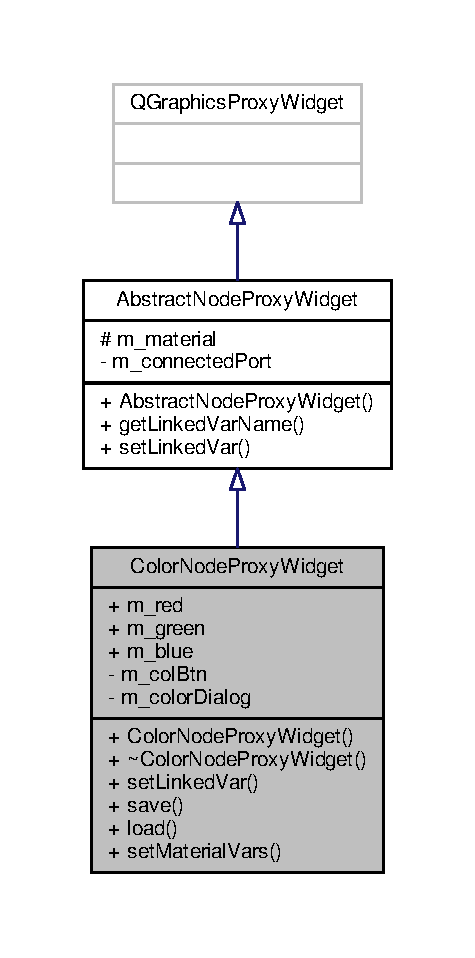
\includegraphics[width=228pt]{class_color_node_proxy_widget__inherit__graph}
\end{center}
\end{figure}


Collaboration diagram for Color\-Node\-Proxy\-Widget\-:
\nopagebreak
\begin{figure}[H]
\begin{center}
\leavevmode
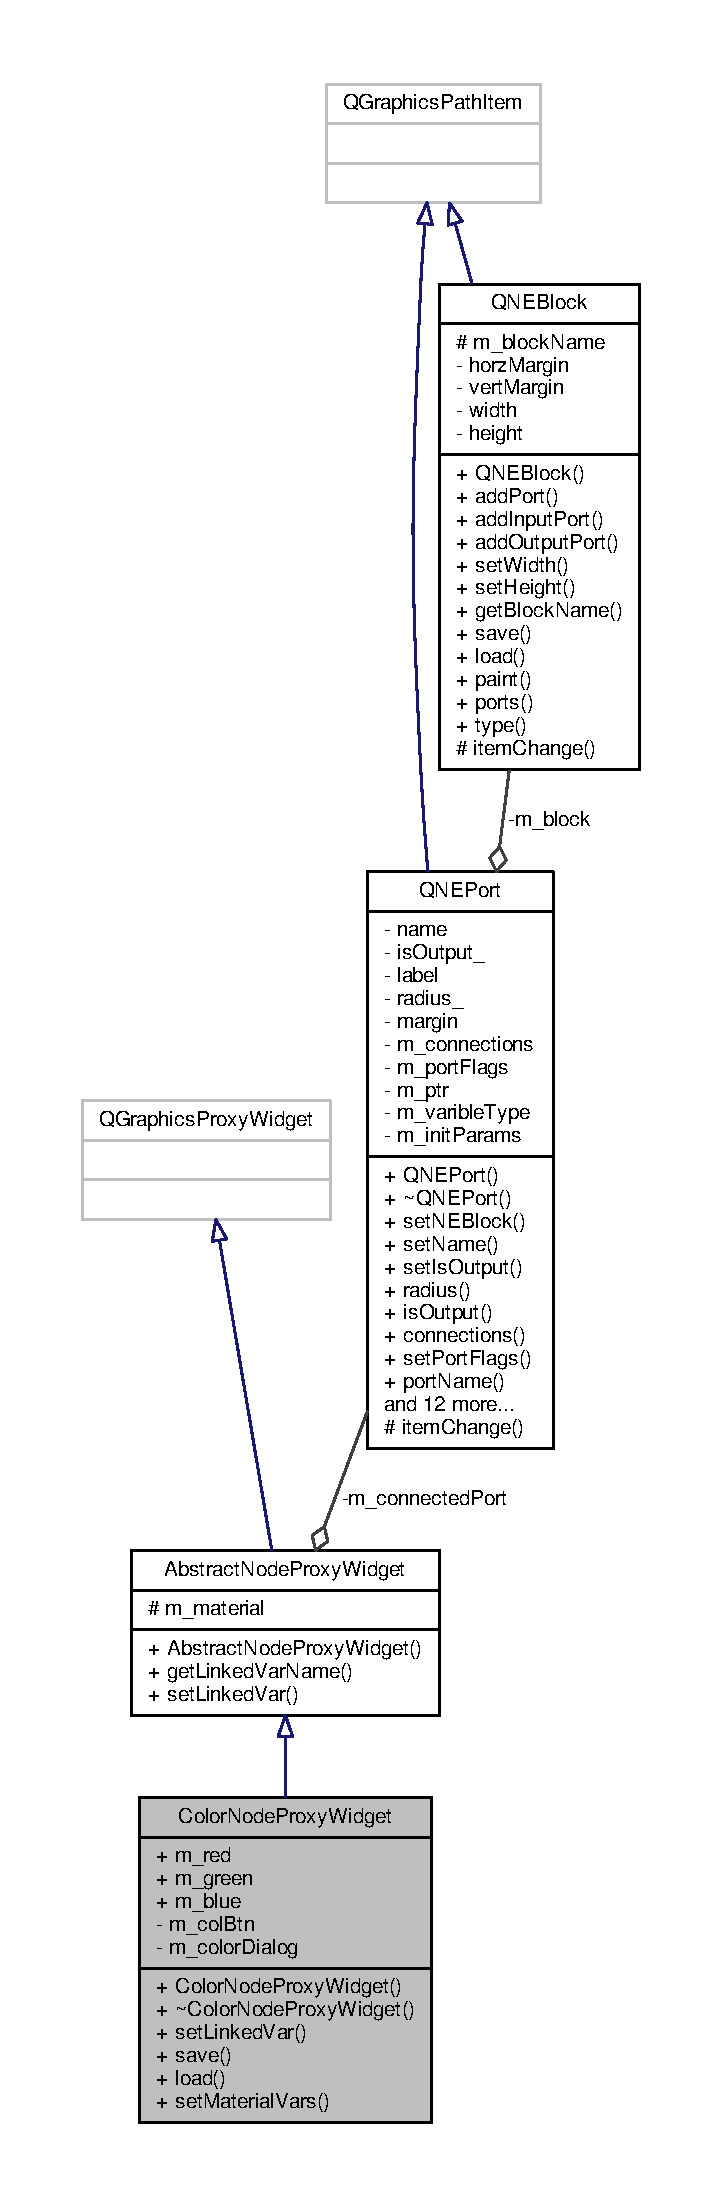
\includegraphics[height=550pt]{class_color_node_proxy_widget__coll__graph}
\end{center}
\end{figure}
\subsection*{Public Slots}
\begin{DoxyCompactItemize}
\item 
void \hyperlink{class_color_node_proxy_widget_add07d21a9e816205e9771214ec2fa6f4}{set\-Material\-Vars} (Q\-Color \-\_\-col)
\begin{DoxyCompactList}\small\item\em a slot to set the varibles in our material when our spin box values is changed \end{DoxyCompactList}\end{DoxyCompactItemize}
\subsection*{Public Member Functions}
\begin{DoxyCompactItemize}
\item 
\hypertarget{class_color_node_proxy_widget_a7a3ed9e2294413a74f5f1470df0fd5c8}{\hyperlink{class_color_node_proxy_widget_a7a3ed9e2294413a74f5f1470df0fd5c8}{Color\-Node\-Proxy\-Widget} (\hyperlink{class_q_n_e_port}{Q\-N\-E\-Port} $\ast$\-\_\-port\-Connected, optix\-::\-Material \&\-\_\-mat, Q\-Graphics\-Item $\ast$parent=0)}\label{class_color_node_proxy_widget_a7a3ed9e2294413a74f5f1470df0fd5c8}

\begin{DoxyCompactList}\small\item\em default constructor \end{DoxyCompactList}\item 
\hypertarget{class_color_node_proxy_widget_a88d96309b54f772c61bbb9861587f444}{\hyperlink{class_color_node_proxy_widget_a88d96309b54f772c61bbb9861587f444}{$\sim$\-Color\-Node\-Proxy\-Widget} ()}\label{class_color_node_proxy_widget_a88d96309b54f772c61bbb9861587f444}

\begin{DoxyCompactList}\small\item\em defualt destructor \end{DoxyCompactList}\item 
\hypertarget{class_color_node_proxy_widget_aba24c0f8211c399c29c458a8ee0dd912}{void \hyperlink{class_color_node_proxy_widget_aba24c0f8211c399c29c458a8ee0dd912}{set\-Linked\-Var} ()}\label{class_color_node_proxy_widget_aba24c0f8211c399c29c458a8ee0dd912}

\begin{DoxyCompactList}\small\item\em overite our set\-Linked\-Var function to put our own functionality in \end{DoxyCompactList}\item 
\hypertarget{class_color_node_proxy_widget_a77c04ecaa265462cf7c06ffaab801c7e}{void \hyperlink{class_color_node_proxy_widget_a77c04ecaa265462cf7c06ffaab801c7e}{save} (Q\-Data\-Stream \&ds)}\label{class_color_node_proxy_widget_a77c04ecaa265462cf7c06ffaab801c7e}

\begin{DoxyCompactList}\small\item\em overload our save function for float 3 node implimentation \end{DoxyCompactList}\item 
\hypertarget{class_color_node_proxy_widget_acf3559d410469d180d064d9e352ccbcb}{void \hyperlink{class_color_node_proxy_widget_acf3559d410469d180d064d9e352ccbcb}{load} (Q\-Data\-Stream \&, Q\-Map$<$ quint64, \hyperlink{class_q_n_e_port}{Q\-N\-E\-Port} $\ast$ $>$ \&port\-Map)}\label{class_color_node_proxy_widget_acf3559d410469d180d064d9e352ccbcb}

\begin{DoxyCompactList}\small\item\em overload our load function for float 3 node implimentation \end{DoxyCompactList}\end{DoxyCompactItemize}
\subsection*{Public Attributes}
\begin{DoxyCompactItemize}
\item 
\hypertarget{class_color_node_proxy_widget_a8c47703e34c239ffb18833a3eb734fe6}{float \hyperlink{class_color_node_proxy_widget_a8c47703e34c239ffb18833a3eb734fe6}{m\-\_\-red}}\label{class_color_node_proxy_widget_a8c47703e34c239ffb18833a3eb734fe6}

\begin{DoxyCompactList}\small\item\em red intensity \end{DoxyCompactList}\item 
\hypertarget{class_color_node_proxy_widget_aa28cea0795b16ec5834e1b4aedc6100e}{float \hyperlink{class_color_node_proxy_widget_aa28cea0795b16ec5834e1b4aedc6100e}{m\-\_\-green}}\label{class_color_node_proxy_widget_aa28cea0795b16ec5834e1b4aedc6100e}

\begin{DoxyCompactList}\small\item\em green intensity \end{DoxyCompactList}\item 
\hypertarget{class_color_node_proxy_widget_a7d819513b88223e46a2740b9528cbd44}{float \hyperlink{class_color_node_proxy_widget_a7d819513b88223e46a2740b9528cbd44}{m\-\_\-blue}}\label{class_color_node_proxy_widget_a7d819513b88223e46a2740b9528cbd44}

\begin{DoxyCompactList}\small\item\em blue intensity \end{DoxyCompactList}\end{DoxyCompactItemize}
\subsection*{Private Attributes}
\begin{DoxyCompactItemize}
\item 
\hypertarget{class_color_node_proxy_widget_a68395843f6fcae8ef7995388a309930c}{Q\-Push\-Button $\ast$ \hyperlink{class_color_node_proxy_widget_a68395843f6fcae8ef7995388a309930c}{m\-\_\-col\-Btn}}\label{class_color_node_proxy_widget_a68395843f6fcae8ef7995388a309930c}

\begin{DoxyCompactList}\small\item\em our colour button \end{DoxyCompactList}\item 
\hypertarget{class_color_node_proxy_widget_a6bdf3c7038a0e52fc1f293fcb04dd28c}{Q\-Color\-Dialog $\ast$ \hyperlink{class_color_node_proxy_widget_a6bdf3c7038a0e52fc1f293fcb04dd28c}{m\-\_\-color\-Dialog}}\label{class_color_node_proxy_widget_a6bdf3c7038a0e52fc1f293fcb04dd28c}

\begin{DoxyCompactList}\small\item\em Color Dialog widget. \end{DoxyCompactList}\end{DoxyCompactItemize}
\subsection*{Additional Inherited Members}


\subsection{Detailed Description}
Extention of \hyperlink{class_abstract_node_proxy_widget}{Abstract\-Node\-Proxy\-Widget} that allows us to select a color and apply it to a attribute of a material. 

Extension of Q\-N\-Eblock, This Abstract class provides a basis for all variable blocks to be drawn in our scene.

\begin{DoxyAuthor}{Author}
Declan Russell 
\end{DoxyAuthor}
\begin{DoxyDate}{Date}
05/05/2015 
\end{DoxyDate}


\subsection{Member Function Documentation}
\hypertarget{class_color_node_proxy_widget_add07d21a9e816205e9771214ec2fa6f4}{\index{Color\-Node\-Proxy\-Widget@{Color\-Node\-Proxy\-Widget}!set\-Material\-Vars@{set\-Material\-Vars}}
\index{set\-Material\-Vars@{set\-Material\-Vars}!ColorNodeProxyWidget@{Color\-Node\-Proxy\-Widget}}
\subsubsection[{set\-Material\-Vars}]{\setlength{\rightskip}{0pt plus 5cm}void Color\-Node\-Proxy\-Widget\-::set\-Material\-Vars (
\begin{DoxyParamCaption}
\item[{Q\-Color}]{\-\_\-col}
\end{DoxyParamCaption}
)\hspace{0.3cm}{\ttfamily [slot]}}}\label{class_color_node_proxy_widget_add07d21a9e816205e9771214ec2fa6f4}


a slot to set the varibles in our material when our spin box values is changed 


\begin{DoxyParams}{Parameters}
{\em \-\_\-col} & -\/ color selected \\
\hline
\end{DoxyParams}


Here is the call graph for this function\-:
\nopagebreak
\begin{figure}[H]
\begin{center}
\leavevmode
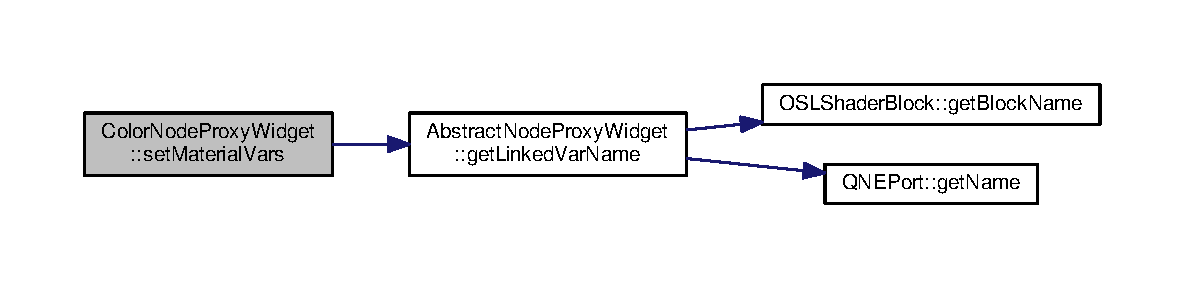
\includegraphics[width=350pt]{class_color_node_proxy_widget_add07d21a9e816205e9771214ec2fa6f4_cgraph}
\end{center}
\end{figure}




Here is the caller graph for this function\-:
\nopagebreak
\begin{figure}[H]
\begin{center}
\leavevmode
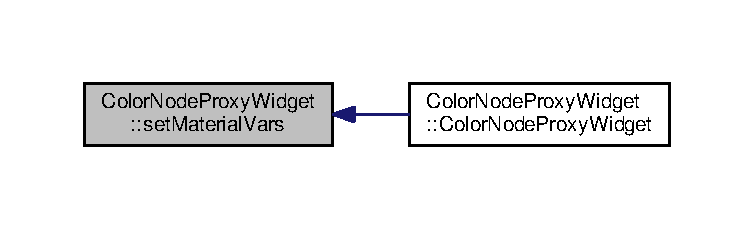
\includegraphics[width=350pt]{class_color_node_proxy_widget_add07d21a9e816205e9771214ec2fa6f4_icgraph}
\end{center}
\end{figure}




The documentation for this class was generated from the following files\-:\begin{DoxyCompactItemize}
\item 
include/\-Node\-Graph/Color\-Node\-Proxy\-Widget.\-h\item 
src/\-Node\-Graph/Color\-Node\-Proxy\-Widget.\-cpp\end{DoxyCompactItemize}

\hypertarget{class_float_node_proxy_widget}{\section{Float\-Node\-Proxy\-Widget Class Reference}
\label{class_float_node_proxy_widget}\index{Float\-Node\-Proxy\-Widget@{Float\-Node\-Proxy\-Widget}}
}


Extention of \hyperlink{class_abstract_node_proxy_widget}{Abstract\-Node\-Proxy\-Widget} that allows us to select a float and apply it to a attribute of a material.  




{\ttfamily \#include $<$Float\-Node\-Proxy\-Widget.\-h$>$}



Inheritance diagram for Float\-Node\-Proxy\-Widget\-:
\nopagebreak
\begin{figure}[H]
\begin{center}
\leavevmode
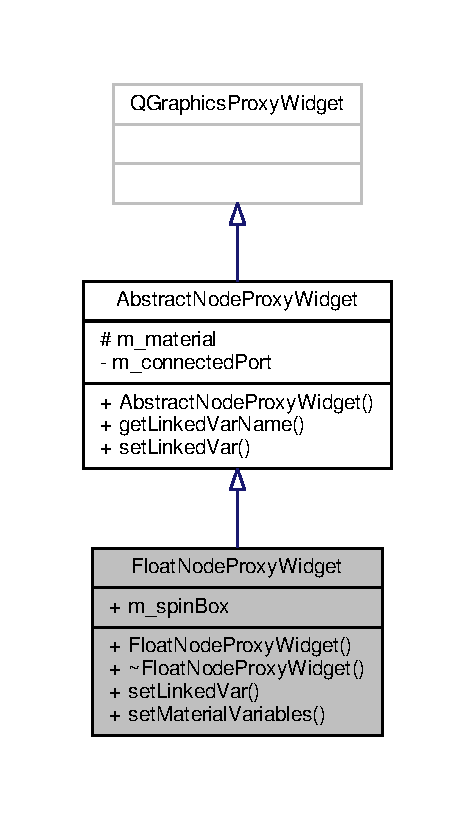
\includegraphics[width=228pt]{class_float_node_proxy_widget__inherit__graph}
\end{center}
\end{figure}


Collaboration diagram for Float\-Node\-Proxy\-Widget\-:
\nopagebreak
\begin{figure}[H]
\begin{center}
\leavevmode
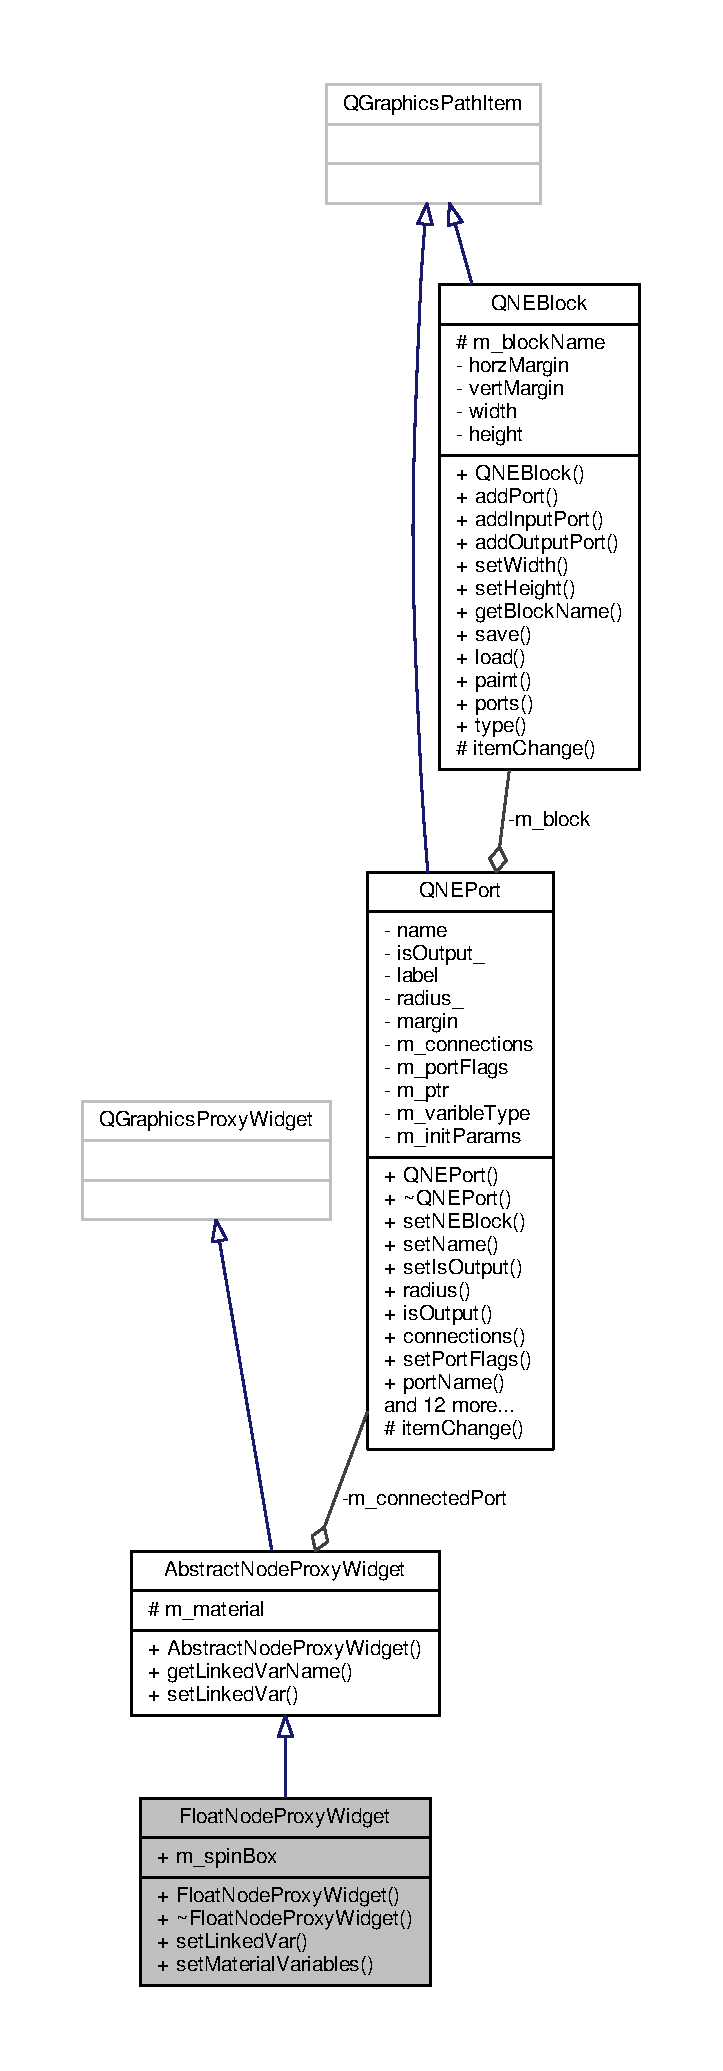
\includegraphics[height=550pt]{class_float_node_proxy_widget__coll__graph}
\end{center}
\end{figure}
\subsection*{Public Slots}
\begin{DoxyCompactItemize}
\item 
void \hyperlink{class_float_node_proxy_widget_af2534a2cae437c7b5c123d52315d0fbf}{set\-Material\-Variables} (double \-\_\-val)
\begin{DoxyCompactList}\small\item\em slot to set the varible in our material when our spin box value is changed \end{DoxyCompactList}\end{DoxyCompactItemize}
\subsection*{Public Member Functions}
\begin{DoxyCompactItemize}
\item 
\hypertarget{class_float_node_proxy_widget_af7146e6a3a5c285d37531d9ce33ba19c}{{\bfseries Float\-Node\-Proxy\-Widget} (\hyperlink{class_q_n_e_port}{Q\-N\-E\-Port} $\ast$\-\_\-port\-Connected, optix\-::\-Material \&\-\_\-mat, Q\-Graphics\-Item $\ast$parent=0)}\label{class_float_node_proxy_widget_af7146e6a3a5c285d37531d9ce33ba19c}

\item 
\hypertarget{class_float_node_proxy_widget_a32f81dfe40973640f0febe2617d38cf5}{\hyperlink{class_float_node_proxy_widget_a32f81dfe40973640f0febe2617d38cf5}{$\sim$\-Float\-Node\-Proxy\-Widget} ()}\label{class_float_node_proxy_widget_a32f81dfe40973640f0febe2617d38cf5}

\begin{DoxyCompactList}\small\item\em default destructor \end{DoxyCompactList}\item 
\hypertarget{class_float_node_proxy_widget_aba0f4178a27b9040de1b84ee3ffd71f4}{void \hyperlink{class_float_node_proxy_widget_aba0f4178a27b9040de1b84ee3ffd71f4}{set\-Linked\-Var} ()}\label{class_float_node_proxy_widget_aba0f4178a27b9040de1b84ee3ffd71f4}

\begin{DoxyCompactList}\small\item\em overite our set\-Linked\-Var function to put our own functionality in \end{DoxyCompactList}\end{DoxyCompactItemize}
\subsection*{Public Attributes}
\begin{DoxyCompactItemize}
\item 
\hypertarget{class_float_node_proxy_widget_a9ce5875eba5a01b81af74d2e30d117c3}{Q\-Double\-Spin\-Box $\ast$ \hyperlink{class_float_node_proxy_widget_a9ce5875eba5a01b81af74d2e30d117c3}{m\-\_\-spin\-Box}}\label{class_float_node_proxy_widget_a9ce5875eba5a01b81af74d2e30d117c3}

\begin{DoxyCompactList}\small\item\em a member for our spin box \end{DoxyCompactList}\end{DoxyCompactItemize}
\subsection*{Additional Inherited Members}


\subsection{Detailed Description}
Extention of \hyperlink{class_abstract_node_proxy_widget}{Abstract\-Node\-Proxy\-Widget} that allows us to select a float and apply it to a attribute of a material. 

This widget consists of a single Double spinbox to input a float value. \begin{DoxyAuthor}{Author}
Declan Russell 
\end{DoxyAuthor}
\begin{DoxyDate}{Date}
05/05/2015 
\end{DoxyDate}


\subsection{Member Function Documentation}
\hypertarget{class_float_node_proxy_widget_af2534a2cae437c7b5c123d52315d0fbf}{\index{Float\-Node\-Proxy\-Widget@{Float\-Node\-Proxy\-Widget}!set\-Material\-Variables@{set\-Material\-Variables}}
\index{set\-Material\-Variables@{set\-Material\-Variables}!FloatNodeProxyWidget@{Float\-Node\-Proxy\-Widget}}
\subsubsection[{set\-Material\-Variables}]{\setlength{\rightskip}{0pt plus 5cm}void Float\-Node\-Proxy\-Widget\-::set\-Material\-Variables (
\begin{DoxyParamCaption}
\item[{double}]{\-\_\-val}
\end{DoxyParamCaption}
)\hspace{0.3cm}{\ttfamily [slot]}}}\label{class_float_node_proxy_widget_af2534a2cae437c7b5c123d52315d0fbf}


slot to set the varible in our material when our spin box value is changed 


\begin{DoxyParams}{Parameters}
{\em \-\_\-val} & the value to set the variables in our material \\
\hline
\end{DoxyParams}


Here is the call graph for this function\-:
\nopagebreak
\begin{figure}[H]
\begin{center}
\leavevmode
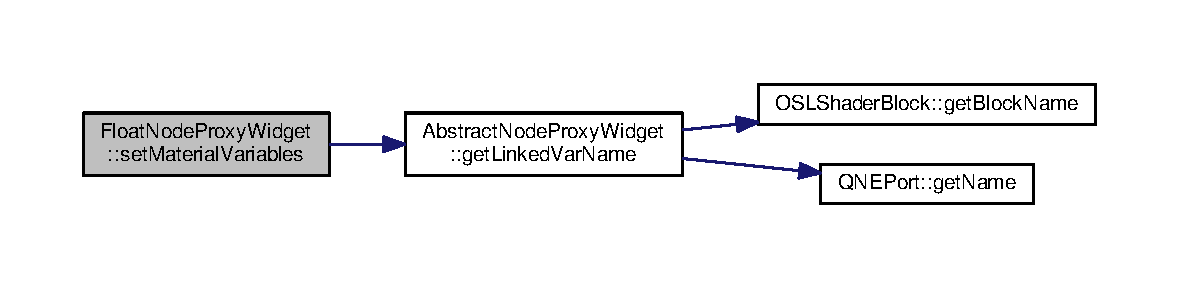
\includegraphics[width=350pt]{class_float_node_proxy_widget_af2534a2cae437c7b5c123d52315d0fbf_cgraph}
\end{center}
\end{figure}




The documentation for this class was generated from the following files\-:\begin{DoxyCompactItemize}
\item 
include/\-Node\-Graph/Float\-Node\-Proxy\-Widget.\-h\item 
src/\-Node\-Graph/Float\-Node\-Proxy\-Widget.\-cpp\end{DoxyCompactItemize}

\hypertarget{class_float_three_node_proxy_widget}{\section{Float\-Three\-Node\-Proxy\-Widget Class Reference}
\label{class_float_three_node_proxy_widget}\index{Float\-Three\-Node\-Proxy\-Widget@{Float\-Three\-Node\-Proxy\-Widget}}
}


Extention of \hyperlink{class_abstract_node_proxy_widget}{Abstract\-Node\-Proxy\-Widget} that allows us to select 3 floats and apply it to a attribute of a material.  




{\ttfamily \#include $<$Float\-Three\-Node\-Proxy\-Widget.\-h$>$}



Inheritance diagram for Float\-Three\-Node\-Proxy\-Widget\-:
\nopagebreak
\begin{figure}[H]
\begin{center}
\leavevmode
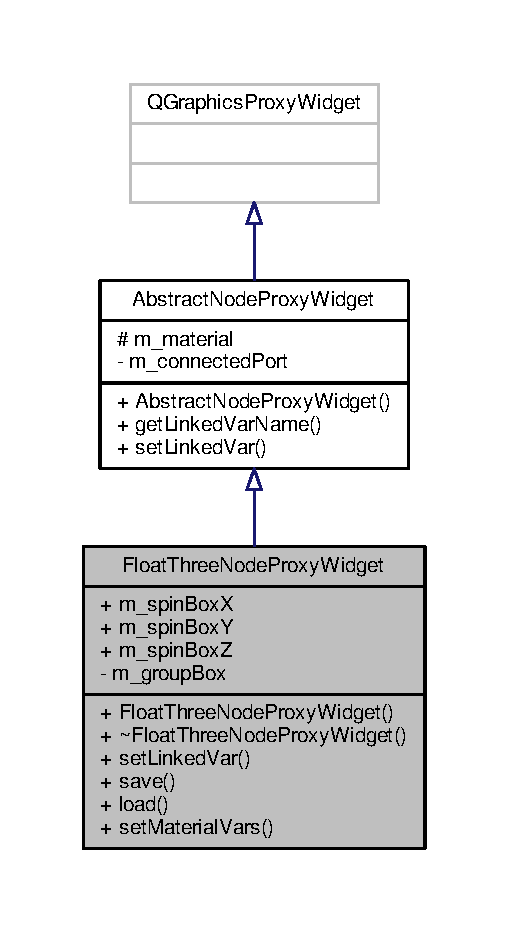
\includegraphics[width=244pt]{class_float_three_node_proxy_widget__inherit__graph}
\end{center}
\end{figure}


Collaboration diagram for Float\-Three\-Node\-Proxy\-Widget\-:
\nopagebreak
\begin{figure}[H]
\begin{center}
\leavevmode
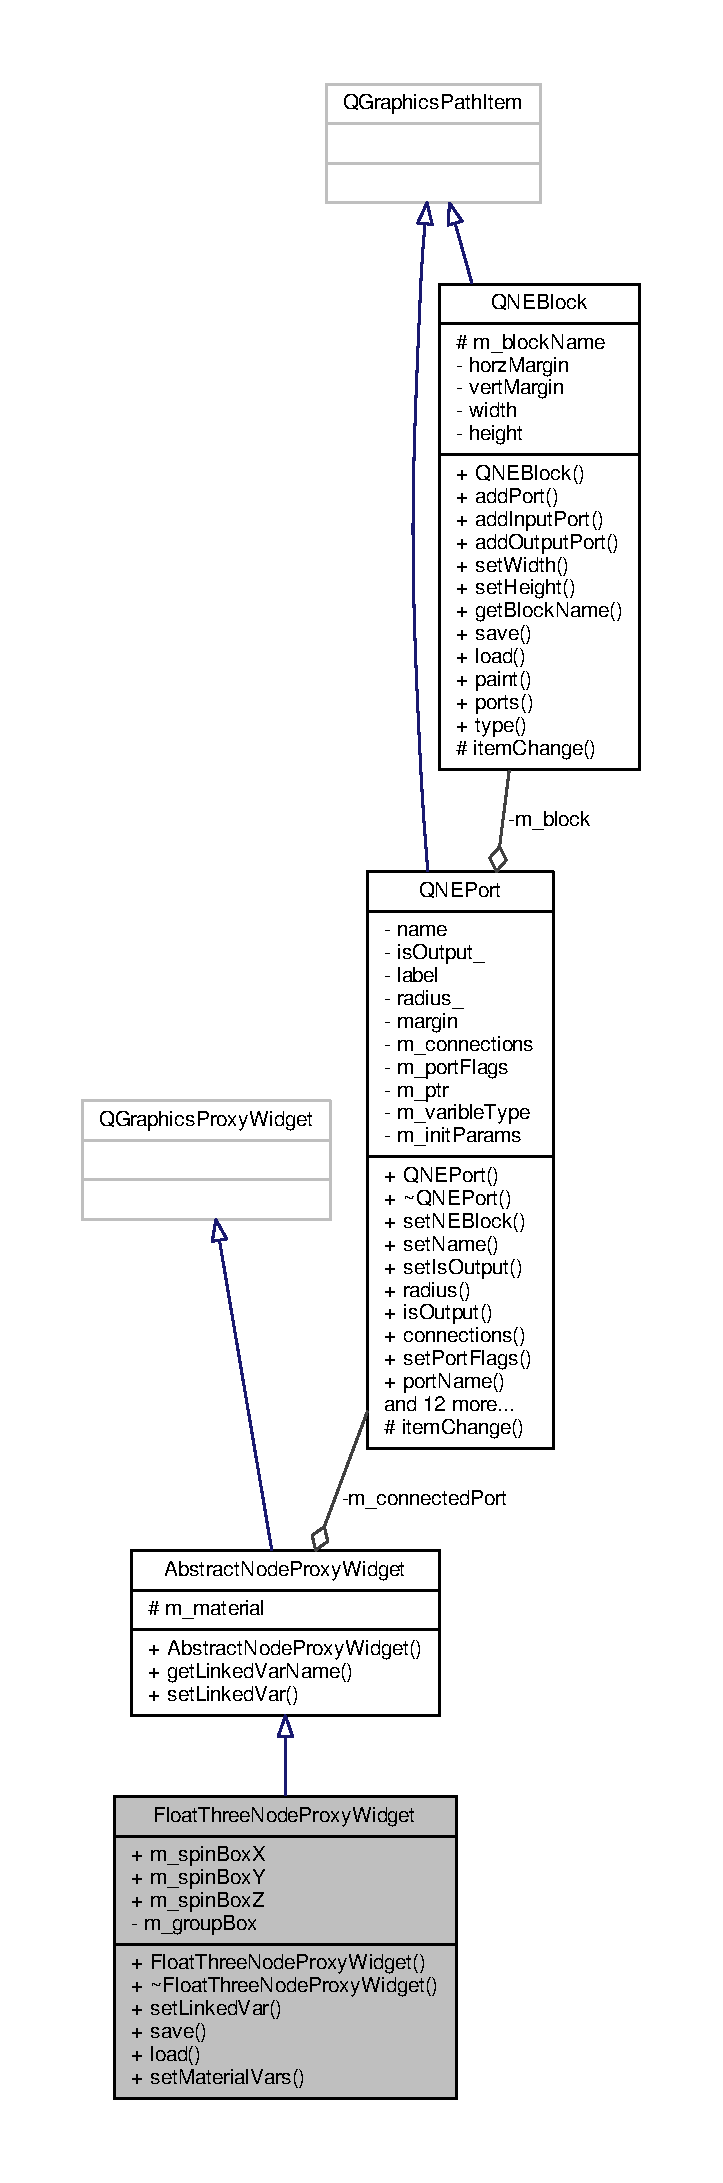
\includegraphics[height=550pt]{class_float_three_node_proxy_widget__coll__graph}
\end{center}
\end{figure}
\subsection*{Public Slots}
\begin{DoxyCompactItemize}
\item 
\hypertarget{class_float_three_node_proxy_widget_afee8481ba8a495ad843429f99b561ecb}{void \hyperlink{class_float_three_node_proxy_widget_afee8481ba8a495ad843429f99b561ecb}{set\-Material\-Vars} ()}\label{class_float_three_node_proxy_widget_afee8481ba8a495ad843429f99b561ecb}

\begin{DoxyCompactList}\small\item\em a slot to set the varibles in our material when our spin box values is changed \end{DoxyCompactList}\end{DoxyCompactItemize}
\subsection*{Public Member Functions}
\begin{DoxyCompactItemize}
\item 
\hyperlink{class_float_three_node_proxy_widget_ac212c5dca46905943b440d47aef9816e}{Float\-Three\-Node\-Proxy\-Widget} (\hyperlink{class_q_n_e_port}{Q\-N\-E\-Port} $\ast$\-\_\-port\-Connected, optix\-::\-Material \&\-\_\-mat, Q\-Graphics\-Item $\ast$parent=0)
\begin{DoxyCompactList}\small\item\em default constructor \end{DoxyCompactList}\item 
\hypertarget{class_float_three_node_proxy_widget_ad56cb8416bf4207dedd542cf5a359d63}{\hyperlink{class_float_three_node_proxy_widget_ad56cb8416bf4207dedd542cf5a359d63}{$\sim$\-Float\-Three\-Node\-Proxy\-Widget} ()}\label{class_float_three_node_proxy_widget_ad56cb8416bf4207dedd542cf5a359d63}

\begin{DoxyCompactList}\small\item\em defualt destructor \end{DoxyCompactList}\item 
\hypertarget{class_float_three_node_proxy_widget_a646dc00d5bf72c2555e0251b58a8b640}{void \hyperlink{class_float_three_node_proxy_widget_a646dc00d5bf72c2555e0251b58a8b640}{set\-Linked\-Var} ()}\label{class_float_three_node_proxy_widget_a646dc00d5bf72c2555e0251b58a8b640}

\begin{DoxyCompactList}\small\item\em overite our set\-Linked\-Var function to put our own functionality in \end{DoxyCompactList}\item 
\hypertarget{class_float_three_node_proxy_widget_afd953a0e2e5ac6f59b7b5c50ecbc7fa9}{void \hyperlink{class_float_three_node_proxy_widget_afd953a0e2e5ac6f59b7b5c50ecbc7fa9}{save} (Q\-Data\-Stream \&ds)}\label{class_float_three_node_proxy_widget_afd953a0e2e5ac6f59b7b5c50ecbc7fa9}

\begin{DoxyCompactList}\small\item\em overload our save function for float 3 node implimentation \end{DoxyCompactList}\item 
\hypertarget{class_float_three_node_proxy_widget_acbbe2ad712df333c00ee33f26b12fc61}{void \hyperlink{class_float_three_node_proxy_widget_acbbe2ad712df333c00ee33f26b12fc61}{load} (Q\-Data\-Stream \&, Q\-Map$<$ quint64, \hyperlink{class_q_n_e_port}{Q\-N\-E\-Port} $\ast$ $>$ \&port\-Map)}\label{class_float_three_node_proxy_widget_acbbe2ad712df333c00ee33f26b12fc61}

\begin{DoxyCompactList}\small\item\em overload our load function for float 3 node implimentation \end{DoxyCompactList}\end{DoxyCompactItemize}
\subsection*{Public Attributes}
\begin{DoxyCompactItemize}
\item 
\hypertarget{class_float_three_node_proxy_widget_af683535cdc97dd14e07fccc72a6466eb}{Q\-Double\-Spin\-Box $\ast$ \hyperlink{class_float_three_node_proxy_widget_af683535cdc97dd14e07fccc72a6466eb}{m\-\_\-spin\-Box\-X}}\label{class_float_three_node_proxy_widget_af683535cdc97dd14e07fccc72a6466eb}

\begin{DoxyCompactList}\small\item\em spinbox for our x component \end{DoxyCompactList}\item 
\hypertarget{class_float_three_node_proxy_widget_a972ce13076c540a1cc01ec8a69e5e725}{Q\-Double\-Spin\-Box $\ast$ \hyperlink{class_float_three_node_proxy_widget_a972ce13076c540a1cc01ec8a69e5e725}{m\-\_\-spin\-Box\-Y}}\label{class_float_three_node_proxy_widget_a972ce13076c540a1cc01ec8a69e5e725}

\begin{DoxyCompactList}\small\item\em spinbox for our y component \end{DoxyCompactList}\item 
\hypertarget{class_float_three_node_proxy_widget_a647eb0ec6918e85d8e2595025a834ad8}{Q\-Double\-Spin\-Box $\ast$ \hyperlink{class_float_three_node_proxy_widget_a647eb0ec6918e85d8e2595025a834ad8}{m\-\_\-spin\-Box\-Z}}\label{class_float_three_node_proxy_widget_a647eb0ec6918e85d8e2595025a834ad8}

\begin{DoxyCompactList}\small\item\em spinbox for our z component \end{DoxyCompactList}\end{DoxyCompactItemize}
\subsection*{Private Attributes}
\begin{DoxyCompactItemize}
\item 
\hypertarget{class_float_three_node_proxy_widget_a584837e3859b1fdadd453ae844d46948}{Q\-Group\-Box $\ast$ \hyperlink{class_float_three_node_proxy_widget_a584837e3859b1fdadd453ae844d46948}{m\-\_\-group\-Box}}\label{class_float_three_node_proxy_widget_a584837e3859b1fdadd453ae844d46948}

\begin{DoxyCompactList}\small\item\em groupbox for our spinbox's to live in \end{DoxyCompactList}\end{DoxyCompactItemize}
\subsection*{Additional Inherited Members}


\subsection{Detailed Description}
Extention of \hyperlink{class_abstract_node_proxy_widget}{Abstract\-Node\-Proxy\-Widget} that allows us to select 3 floats and apply it to a attribute of a material. 

This widget consists of 3 Double Spinbox's. This is to be used for such tripplets as Vectors. \begin{DoxyAuthor}{Author}
Declan Russell 
\end{DoxyAuthor}
\begin{DoxyDate}{Date}
05/05/2015 
\end{DoxyDate}


\subsection{Constructor \& Destructor Documentation}
\hypertarget{class_float_three_node_proxy_widget_ac212c5dca46905943b440d47aef9816e}{\index{Float\-Three\-Node\-Proxy\-Widget@{Float\-Three\-Node\-Proxy\-Widget}!Float\-Three\-Node\-Proxy\-Widget@{Float\-Three\-Node\-Proxy\-Widget}}
\index{Float\-Three\-Node\-Proxy\-Widget@{Float\-Three\-Node\-Proxy\-Widget}!FloatThreeNodeProxyWidget@{Float\-Three\-Node\-Proxy\-Widget}}
\subsubsection[{Float\-Three\-Node\-Proxy\-Widget}]{\setlength{\rightskip}{0pt plus 5cm}Float\-Three\-Node\-Proxy\-Widget\-::\-Float\-Three\-Node\-Proxy\-Widget (
\begin{DoxyParamCaption}
\item[{{\bf Q\-N\-E\-Port} $\ast$}]{\-\_\-port\-Connected, }
\item[{optix\-::\-Material \&}]{\-\_\-mat, }
\item[{Q\-Graphics\-Item $\ast$}]{parent = {\ttfamily 0}}
\end{DoxyParamCaption}
)}}\label{class_float_three_node_proxy_widget_ac212c5dca46905943b440d47aef9816e}


default constructor 

\begin{DoxyRefDesc}{Todo}
\item[\hyperlink{todo__todo000008}{Todo}]comment this class mo! \end{DoxyRefDesc}


Here is the call graph for this function\-:
\nopagebreak
\begin{figure}[H]
\begin{center}
\leavevmode
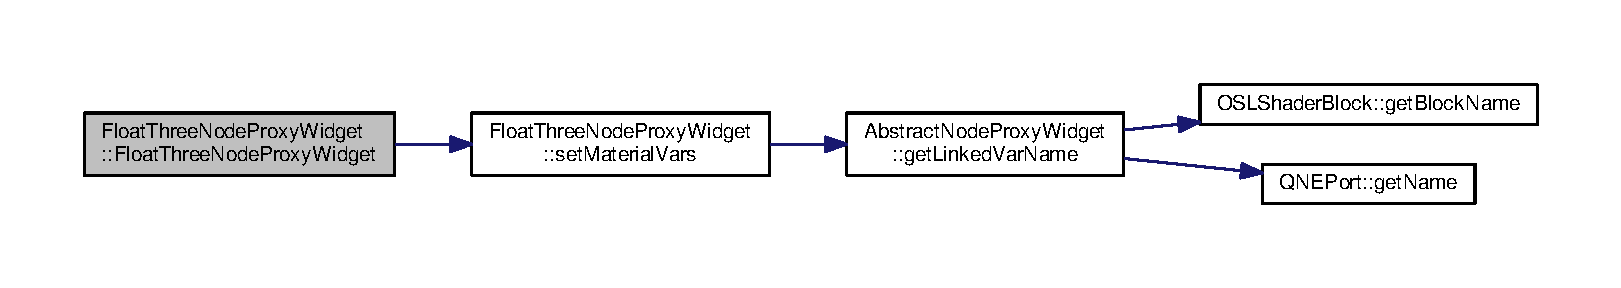
\includegraphics[width=350pt]{class_float_three_node_proxy_widget_ac212c5dca46905943b440d47aef9816e_cgraph}
\end{center}
\end{figure}




The documentation for this class was generated from the following files\-:\begin{DoxyCompactItemize}
\item 
include/\-Node\-Graph/Float\-Three\-Node\-Proxy\-Widget.\-h\item 
src/\-Node\-Graph/Float\-Three\-Node\-Proxy\-Widget.\-cpp\end{DoxyCompactItemize}

\hypertarget{struct_text_1_1_font_char}{\section{Text\-:\-:Font\-Char Struct Reference}
\label{struct_text_1_1_font_char}\index{Text\-::\-Font\-Char@{Text\-::\-Font\-Char}}
}


a structure to hold the font char texture id and the vao. The vao for each font will be a different size need to investigate is a scale would be quicker / more efficient than storing multiple billboards (some will be the same size)  




{\ttfamily \#include $<$Text.\-h$>$}



Collaboration diagram for Text\-:\-:Font\-Char\-:
\nopagebreak
\begin{figure}[H]
\begin{center}
\leavevmode
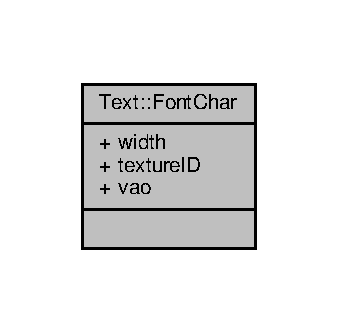
\includegraphics[width=162pt]{struct_text_1_1_font_char__coll__graph}
\end{center}
\end{figure}
\subsection*{Public Attributes}
\begin{DoxyCompactItemize}
\item 
\hypertarget{struct_text_1_1_font_char_abbf7e80a16c3190894c5a9e195180bd8}{int {\bfseries width}}\label{struct_text_1_1_font_char_abbf7e80a16c3190894c5a9e195180bd8}

\item 
\hypertarget{struct_text_1_1_font_char_a7ef075790be18e9bac4bfbb56b528428}{G\-Luint \hyperlink{struct_text_1_1_font_char_a7ef075790be18e9bac4bfbb56b528428}{texture\-I\-D}}\label{struct_text_1_1_font_char_a7ef075790be18e9bac4bfbb56b528428}

\begin{DoxyCompactList}\small\item\em the width of the font \end{DoxyCompactList}\item 
\hypertarget{struct_text_1_1_font_char_a763c6e3ecbe30d33becd27b8c7310d39}{G\-Luint \hyperlink{struct_text_1_1_font_char_a763c6e3ecbe30d33becd27b8c7310d39}{vao}}\label{struct_text_1_1_font_char_a763c6e3ecbe30d33becd27b8c7310d39}

\begin{DoxyCompactList}\small\item\em the texture id of the font billboard \end{DoxyCompactList}\end{DoxyCompactItemize}


\subsection{Detailed Description}
a structure to hold the font char texture id and the vao. The vao for each font will be a different size need to investigate is a scale would be quicker / more efficient than storing multiple billboards (some will be the same size) 

The documentation for this struct was generated from the following file\-:\begin{DoxyCompactItemize}
\item 
include/\-Core/\hyperlink{_text_8h}{Text.\-h}\end{DoxyCompactItemize}

\hypertarget{struct_for_loop}{\section{For\-Loop Struct Reference}
\label{struct_for_loop}\index{For\-Loop@{For\-Loop}}
}


A structure to hold jump targets for use will for loops.  




{\ttfamily \#include $<$Oso\-Reader.\-h$>$}



Collaboration diagram for For\-Loop\-:
\nopagebreak
\begin{figure}[H]
\begin{center}
\leavevmode
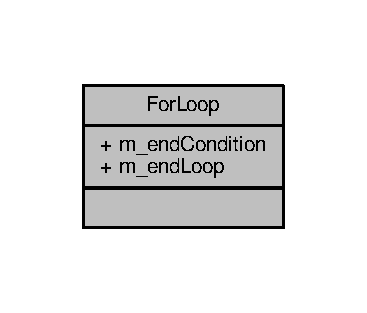
\includegraphics[width=176pt]{struct_for_loop__coll__graph}
\end{center}
\end{figure}
\subsection*{Public Attributes}
\begin{DoxyCompactItemize}
\item 
\hypertarget{struct_for_loop_aaef7e31074d40bf7b19e49b93351ac58}{int {\bfseries m\-\_\-end\-Condition}}\label{struct_for_loop_aaef7e31074d40bf7b19e49b93351ac58}

\item 
\hypertarget{struct_for_loop_a3480ffbbf6537330ed26e7925f4a10e9}{int {\bfseries m\-\_\-end\-Loop}}\label{struct_for_loop_a3480ffbbf6537330ed26e7925f4a10e9}

\end{DoxyCompactItemize}


\subsection{Detailed Description}
A structure to hold jump targets for use will for loops. 

The documentation for this struct was generated from the following file\-:\begin{DoxyCompactItemize}
\item 
include/\-O\-S\-L\-Compiler/Oso\-Reader.\-h\end{DoxyCompactItemize}

\hypertarget{class_gen_set_dock_widget}{\section{Gen\-Set\-Dock\-Widget Class Reference}
\label{class_gen_set_dock_widget}\index{Gen\-Set\-Dock\-Widget@{Gen\-Set\-Dock\-Widget}}
}


Inheritance diagram for Gen\-Set\-Dock\-Widget\-:
\nopagebreak
\begin{figure}[H]
\begin{center}
\leavevmode
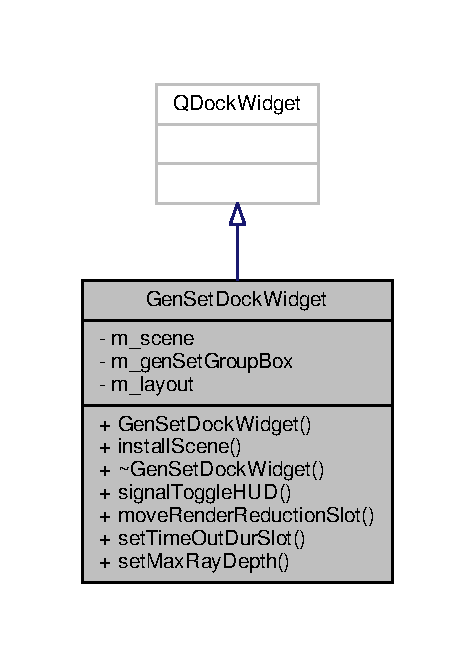
\includegraphics[width=228pt]{class_gen_set_dock_widget__inherit__graph}
\end{center}
\end{figure}


Collaboration diagram for Gen\-Set\-Dock\-Widget\-:
\nopagebreak
\begin{figure}[H]
\begin{center}
\leavevmode
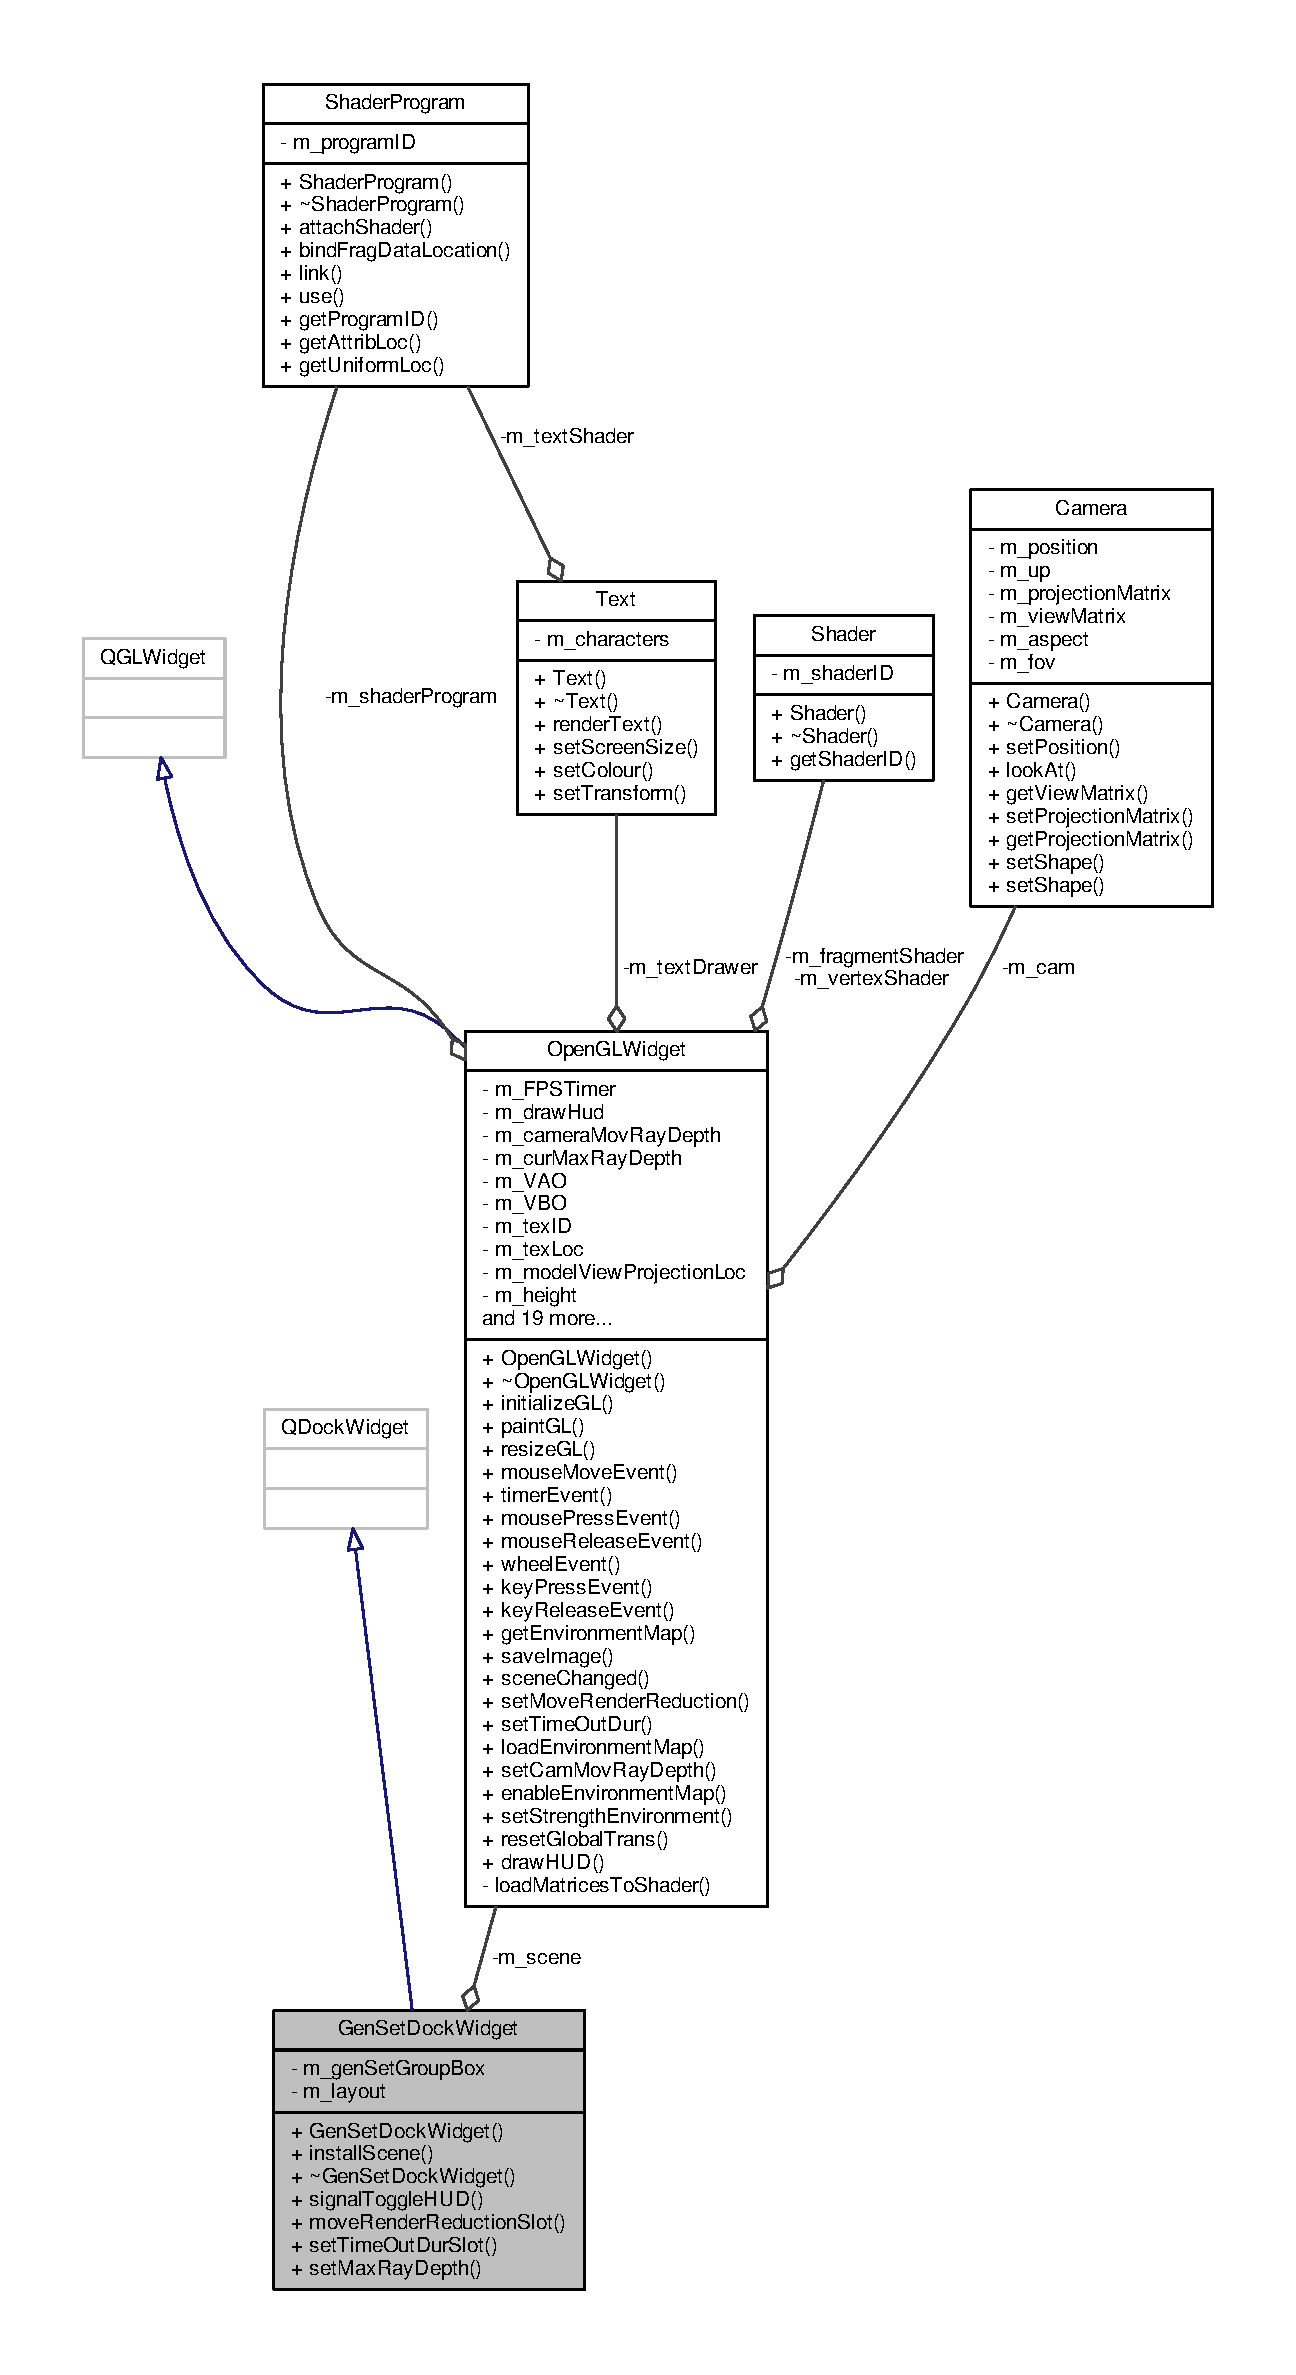
\includegraphics[height=550pt]{class_gen_set_dock_widget__coll__graph}
\end{center}
\end{figure}
\subsection*{Public Slots}
\begin{DoxyCompactItemize}
\item 
\hypertarget{class_gen_set_dock_widget_a386643c3cae291d03f1ebb51de73b5e3}{void \hyperlink{class_gen_set_dock_widget_a386643c3cae291d03f1ebb51de73b5e3}{signal\-Toggle\-H\-U\-D} (bool \-\_\-toggle)}\label{class_gen_set_dock_widget_a386643c3cae291d03f1ebb51de73b5e3}

\begin{DoxyCompactList}\small\item\em slot to signal toggle of H\-U\-D \end{DoxyCompactList}\item 
\hypertarget{class_gen_set_dock_widget_a32cd3765a3e10a384aef77177bc5eb55}{void \hyperlink{class_gen_set_dock_widget_a32cd3765a3e10a384aef77177bc5eb55}{move\-Render\-Reduction\-Slot} (int \-\_\-reduction\-Amount)}\label{class_gen_set_dock_widget_a32cd3765a3e10a384aef77177bc5eb55}

\begin{DoxyCompactList}\small\item\em slot to call change in movement render reduction \end{DoxyCompactList}\item 
\hypertarget{class_gen_set_dock_widget_a95fc0877239b23721c1d0db71793bf9e}{void \hyperlink{class_gen_set_dock_widget_a95fc0877239b23721c1d0db71793bf9e}{set\-Time\-Out\-Dur\-Slot} (int \-\_\-timeout)}\label{class_gen_set_dock_widget_a95fc0877239b23721c1d0db71793bf9e}

\begin{DoxyCompactList}\small\item\em slot to call change in timeout \end{DoxyCompactList}\item 
void \hyperlink{class_gen_set_dock_widget_a1c26ee85a7c8734aa70472466f4777a7}{set\-Max\-Ray\-Depth} (int \-\_\-depth)
\begin{DoxyCompactList}\small\item\em slot to set the max ray depth \end{DoxyCompactList}\end{DoxyCompactItemize}
\subsection*{Signals}
\begin{DoxyCompactItemize}
\item 
\hypertarget{class_gen_set_dock_widget_abe2429dbc481993e9b2898825db10681}{void \hyperlink{class_gen_set_dock_widget_abe2429dbc481993e9b2898825db10681}{signal\-Move\-Render\-Reduction} (int \-\_\-reduction\-Amount)}\label{class_gen_set_dock_widget_abe2429dbc481993e9b2898825db10681}

\begin{DoxyCompactList}\small\item\em a signal to change the movement render reduction \end{DoxyCompactList}\item 
\hypertarget{class_gen_set_dock_widget_ab8453a51013749869de98a5f4e863e2c}{void \hyperlink{class_gen_set_dock_widget_ab8453a51013749869de98a5f4e863e2c}{signal\-Set\-Time\-Out\-Dur} (int \-\_\-timeout)}\label{class_gen_set_dock_widget_ab8453a51013749869de98a5f4e863e2c}

\begin{DoxyCompactList}\small\item\em a signal to change our time our duration \end{DoxyCompactList}\item 
\hypertarget{class_gen_set_dock_widget_a6b8f743a49dbb2a6d624668cddfd58c5}{void \hyperlink{class_gen_set_dock_widget_a6b8f743a49dbb2a6d624668cddfd58c5}{toggle\-H\-U\-D} (bool \-\_\-toggle)}\label{class_gen_set_dock_widget_a6b8f743a49dbb2a6d624668cddfd58c5}

\begin{DoxyCompactList}\small\item\em signal to toggle H\-U\-D \end{DoxyCompactList}\end{DoxyCompactItemize}
\subsection*{Public Member Functions}
\begin{DoxyCompactItemize}
\item 
\hypertarget{class_gen_set_dock_widget_a438953fb1560e6b04895023cdc805e00}{\hyperlink{class_gen_set_dock_widget_a438953fb1560e6b04895023cdc805e00}{Gen\-Set\-Dock\-Widget} (Q\-Widget $\ast$parent=0)}\label{class_gen_set_dock_widget_a438953fb1560e6b04895023cdc805e00}

\begin{DoxyCompactList}\small\item\em our default constructor \end{DoxyCompactList}\item 
\hypertarget{class_gen_set_dock_widget_a999341b74bebe79f7e1b95e5f0aa1f6c}{void \hyperlink{class_gen_set_dock_widget_a999341b74bebe79f7e1b95e5f0aa1f6c}{install\-Scene} (\hyperlink{class_open_g_l_widget}{Open\-G\-L\-Widget} $\ast$\-\_\-scene)}\label{class_gen_set_dock_widget_a999341b74bebe79f7e1b95e5f0aa1f6c}

\begin{DoxyCompactList}\small\item\em set the scene our general settings apply to \end{DoxyCompactList}\item 
\hypertarget{class_gen_set_dock_widget_a5062abcc91b59ac636cf369ace58c25c}{\hyperlink{class_gen_set_dock_widget_a5062abcc91b59ac636cf369ace58c25c}{$\sim$\-Gen\-Set\-Dock\-Widget} ()}\label{class_gen_set_dock_widget_a5062abcc91b59ac636cf369ace58c25c}

\begin{DoxyCompactList}\small\item\em our destructor \end{DoxyCompactList}\end{DoxyCompactItemize}
\subsection*{Private Attributes}
\begin{DoxyCompactItemize}
\item 
\hypertarget{class_gen_set_dock_widget_ab0bf9289c3a7bb8a01041892ad5dc615}{\hyperlink{class_open_g_l_widget}{Open\-G\-L\-Widget} $\ast$ \hyperlink{class_gen_set_dock_widget_ab0bf9289c3a7bb8a01041892ad5dc615}{m\-\_\-scene}}\label{class_gen_set_dock_widget_ab0bf9289c3a7bb8a01041892ad5dc615}

\begin{DoxyCompactList}\small\item\em our open\-G\-L scene \end{DoxyCompactList}\item 
\hypertarget{class_gen_set_dock_widget_adc7961ca4fa2aa2ec53861b590bc2f49}{Q\-Group\-Box $\ast$ \hyperlink{class_gen_set_dock_widget_adc7961ca4fa2aa2ec53861b590bc2f49}{m\-\_\-gen\-Set\-Group\-Box}}\label{class_gen_set_dock_widget_adc7961ca4fa2aa2ec53861b590bc2f49}

\begin{DoxyCompactList}\small\item\em our group box to hold our controls \end{DoxyCompactList}\item 
\hypertarget{class_gen_set_dock_widget_aa74573626a0acb200d2c70962829ce16}{Q\-Grid\-Layout $\ast$ \hyperlink{class_gen_set_dock_widget_aa74573626a0acb200d2c70962829ce16}{m\-\_\-layout}}\label{class_gen_set_dock_widget_aa74573626a0acb200d2c70962829ce16}

\begin{DoxyCompactList}\small\item\em the layout of our group box widget \end{DoxyCompactList}\end{DoxyCompactItemize}


\subsection{Member Function Documentation}
\hypertarget{class_gen_set_dock_widget_a1c26ee85a7c8734aa70472466f4777a7}{\index{Gen\-Set\-Dock\-Widget@{Gen\-Set\-Dock\-Widget}!set\-Max\-Ray\-Depth@{set\-Max\-Ray\-Depth}}
\index{set\-Max\-Ray\-Depth@{set\-Max\-Ray\-Depth}!GenSetDockWidget@{Gen\-Set\-Dock\-Widget}}
\subsubsection[{set\-Max\-Ray\-Depth}]{\setlength{\rightskip}{0pt plus 5cm}void Gen\-Set\-Dock\-Widget\-::set\-Max\-Ray\-Depth (
\begin{DoxyParamCaption}
\item[{int}]{\-\_\-depth}
\end{DoxyParamCaption}
)\hspace{0.3cm}{\ttfamily [inline]}, {\ttfamily [slot]}}}\label{class_gen_set_dock_widget_a1c26ee85a7c8734aa70472466f4777a7}


slot to set the max ray depth 


\begin{DoxyParams}{Parameters}
{\em \-\_\-depth} & -\/ desired ray depth \\
\hline
\end{DoxyParams}


Here is the call graph for this function\-:
\nopagebreak
\begin{figure}[H]
\begin{center}
\leavevmode
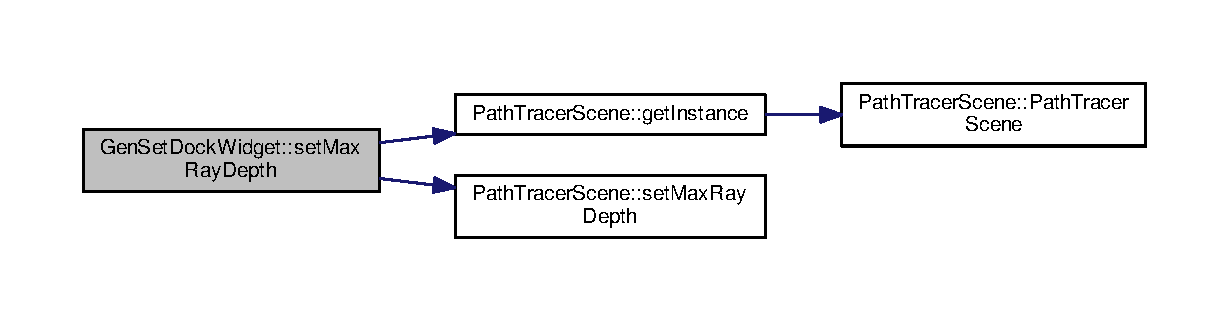
\includegraphics[width=350pt]{class_gen_set_dock_widget_a1c26ee85a7c8734aa70472466f4777a7_cgraph}
\end{center}
\end{figure}




Here is the caller graph for this function\-:
\nopagebreak
\begin{figure}[H]
\begin{center}
\leavevmode
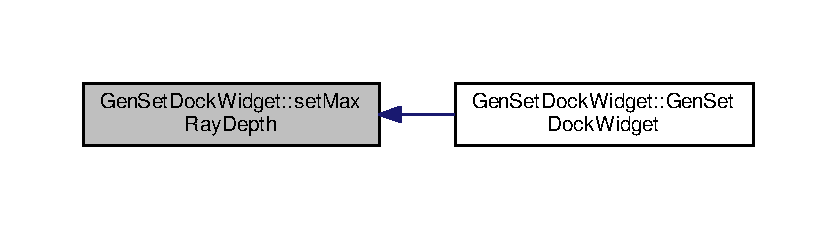
\includegraphics[width=350pt]{class_gen_set_dock_widget_a1c26ee85a7c8734aa70472466f4777a7_icgraph}
\end{center}
\end{figure}




The documentation for this class was generated from the following files\-:\begin{DoxyCompactItemize}
\item 
include/\-U\-I/Gen\-Set\-Dock\-Widget.\-h\item 
moc/moc\-\_\-\-Gen\-Set\-Dock\-Widget.\-cpp\item 
src/\-U\-I/Gen\-Set\-Dock\-Widget.\-cpp\end{DoxyCompactItemize}

\hypertarget{class_gen_set_dock_wiget}{\section{Gen\-Set\-Dock\-Wiget Class Reference}
\label{class_gen_set_dock_wiget}\index{Gen\-Set\-Dock\-Wiget@{Gen\-Set\-Dock\-Wiget}}
}


A Dockable widget which will hold controls to change the general settings of our application.  




{\ttfamily \#include $<$Gen\-Set\-Dock\-Widget.\-h$>$}



Collaboration diagram for Gen\-Set\-Dock\-Wiget\-:
\nopagebreak
\begin{figure}[H]
\begin{center}
\leavevmode
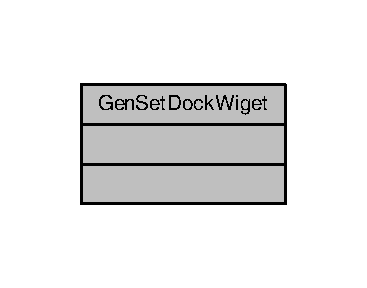
\includegraphics[width=176pt]{class_gen_set_dock_wiget__coll__graph}
\end{center}
\end{figure}


\subsection{Detailed Description}
A Dockable widget which will hold controls to change the general settings of our application. 

\begin{DoxyDate}{Date}
26/02/2015 
\end{DoxyDate}
\begin{DoxyAuthor}{Author}
Declan Russell 
\end{DoxyAuthor}
\begin{DoxyVersion}{Version}
1.\-0 
\end{DoxyVersion}


The documentation for this class was generated from the following file\-:\begin{DoxyCompactItemize}
\item 
include/\-U\-I/Gen\-Set\-Dock\-Widget.\-h\end{DoxyCompactItemize}

\hypertarget{class_h_d_r_loader}{\section{H\-D\-R\-Loader Class Reference}
\label{class_h_d_r_loader}\index{H\-D\-R\-Loader@{H\-D\-R\-Loader}}
}


Collaboration diagram for H\-D\-R\-Loader\-:
\nopagebreak
\begin{figure}[H]
\begin{center}
\leavevmode
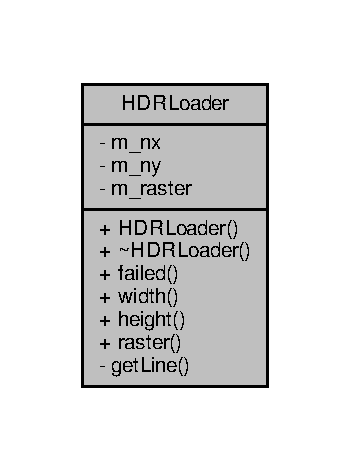
\includegraphics[width=168pt]{class_h_d_r_loader__coll__graph}
\end{center}
\end{figure}
\subsection*{Public Member Functions}
\begin{DoxyCompactItemize}
\item 
\hypertarget{class_h_d_r_loader_a48862ffa3232fa33eb66e678626ecbb3}{S\-U\-T\-I\-L\-A\-P\-I {\bfseries H\-D\-R\-Loader} (const std\-::string \&filename)}\label{class_h_d_r_loader_a48862ffa3232fa33eb66e678626ecbb3}

\item 
\hypertarget{class_h_d_r_loader_a492cd646d50f8091d486ced4da5381a9}{S\-U\-T\-I\-L\-A\-P\-I bool {\bfseries failed} () const }\label{class_h_d_r_loader_a492cd646d50f8091d486ced4da5381a9}

\item 
\hypertarget{class_h_d_r_loader_af515ddb1a7004efaca466613d5ca3a42}{S\-U\-T\-I\-L\-A\-P\-I unsigned int {\bfseries width} () const }\label{class_h_d_r_loader_af515ddb1a7004efaca466613d5ca3a42}

\item 
\hypertarget{class_h_d_r_loader_a05bae772760abfb3809e03509ff93156}{S\-U\-T\-I\-L\-A\-P\-I unsigned int {\bfseries height} () const }\label{class_h_d_r_loader_a05bae772760abfb3809e03509ff93156}

\item 
\hypertarget{class_h_d_r_loader_a7e5196d506b4aee4ecd857c25c742825}{S\-U\-T\-I\-L\-A\-P\-I float $\ast$ {\bfseries raster} () const }\label{class_h_d_r_loader_a7e5196d506b4aee4ecd857c25c742825}

\end{DoxyCompactItemize}
\subsection*{Static Private Member Functions}
\begin{DoxyCompactItemize}
\item 
\hypertarget{class_h_d_r_loader_a663532db9acaf772c4fc2be0607ced2f}{static void {\bfseries get\-Line} (std\-::ifstream \&file\-\_\-in, std\-::string \&s)}\label{class_h_d_r_loader_a663532db9acaf772c4fc2be0607ced2f}

\end{DoxyCompactItemize}
\subsection*{Private Attributes}
\begin{DoxyCompactItemize}
\item 
\hypertarget{class_h_d_r_loader_af369873a0c721da0b84b39e7a97486b4}{unsigned int {\bfseries m\-\_\-nx}}\label{class_h_d_r_loader_af369873a0c721da0b84b39e7a97486b4}

\item 
\hypertarget{class_h_d_r_loader_acc899f9e422fbb4f550ee9aa86521ba9}{unsigned int {\bfseries m\-\_\-ny}}\label{class_h_d_r_loader_acc899f9e422fbb4f550ee9aa86521ba9}

\item 
\hypertarget{class_h_d_r_loader_ab4b7b0ab50869b6bacffc490e3454cdc}{float $\ast$ {\bfseries m\-\_\-raster}}\label{class_h_d_r_loader_ab4b7b0ab50869b6bacffc490e3454cdc}

\end{DoxyCompactItemize}


The documentation for this class was generated from the following files\-:\begin{DoxyCompactItemize}
\item 
include/\-Core/H\-D\-R\-Loader.\-h\item 
src/\-Core/H\-D\-R\-Loader.\-cpp\end{DoxyCompactItemize}

\hypertarget{structhsv}{\section{hsv Struct Reference}
\label{structhsv}\index{hsv@{hsv}}
}


Collaboration diagram for hsv\-:
\nopagebreak
\begin{figure}[H]
\begin{center}
\leavevmode
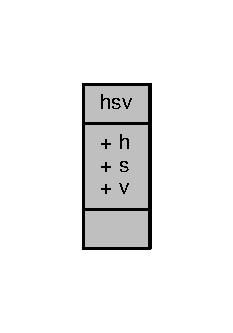
\includegraphics[width=112pt]{structhsv__coll__graph}
\end{center}
\end{figure}
\subsection*{Public Attributes}
\begin{DoxyCompactItemize}
\item 
\hypertarget{structhsv_aa27eea5f2a89b941eead7139330d12f4}{double {\bfseries h}}\label{structhsv_aa27eea5f2a89b941eead7139330d12f4}

\item 
\hypertarget{structhsv_a3cbdc4bf500068b5c4466c4272114a23}{double {\bfseries s}}\label{structhsv_a3cbdc4bf500068b5c4466c4272114a23}

\item 
\hypertarget{structhsv_a572c01d23590231adffe6f9b16df20d3}{double {\bfseries v}}\label{structhsv_a572c01d23590231adffe6f9b16df20d3}

\end{DoxyCompactItemize}


The documentation for this struct was generated from the following file\-:\begin{DoxyCompactItemize}
\item 
src/\-Core/H\-D\-R\-Loader.\-cpp\end{DoxyCompactItemize}

\hypertarget{class_image_node_proxy_widget}{\section{Image\-Node\-Proxy\-Widget Class Reference}
\label{class_image_node_proxy_widget}\index{Image\-Node\-Proxy\-Widget@{Image\-Node\-Proxy\-Widget}}
}


Extention of \hyperlink{class_abstract_node_proxy_widget}{Abstract\-Node\-Proxy\-Widget} that allows us to select an image and apply it to a attribute of a material.  




{\ttfamily \#include $<$Image\-Node\-Proxy\-Widget.\-h$>$}



Inheritance diagram for Image\-Node\-Proxy\-Widget\-:
\nopagebreak
\begin{figure}[H]
\begin{center}
\leavevmode
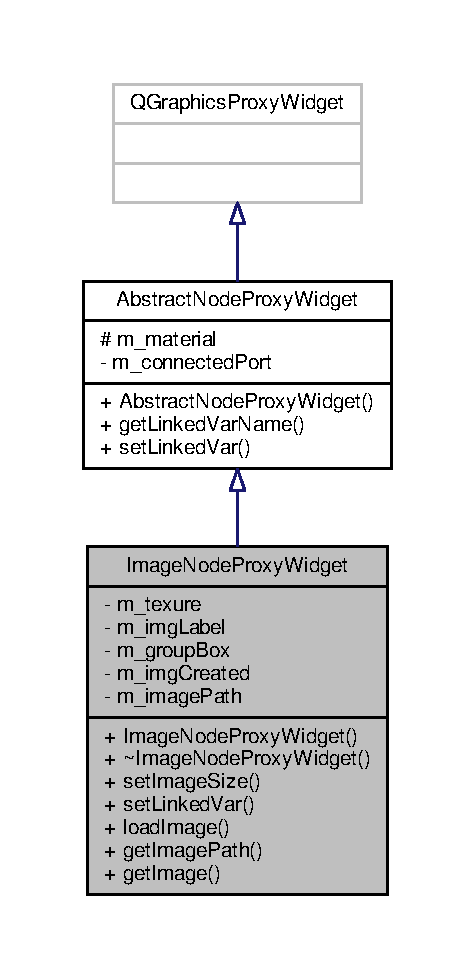
\includegraphics[width=228pt]{class_image_node_proxy_widget__inherit__graph}
\end{center}
\end{figure}


Collaboration diagram for Image\-Node\-Proxy\-Widget\-:
\nopagebreak
\begin{figure}[H]
\begin{center}
\leavevmode
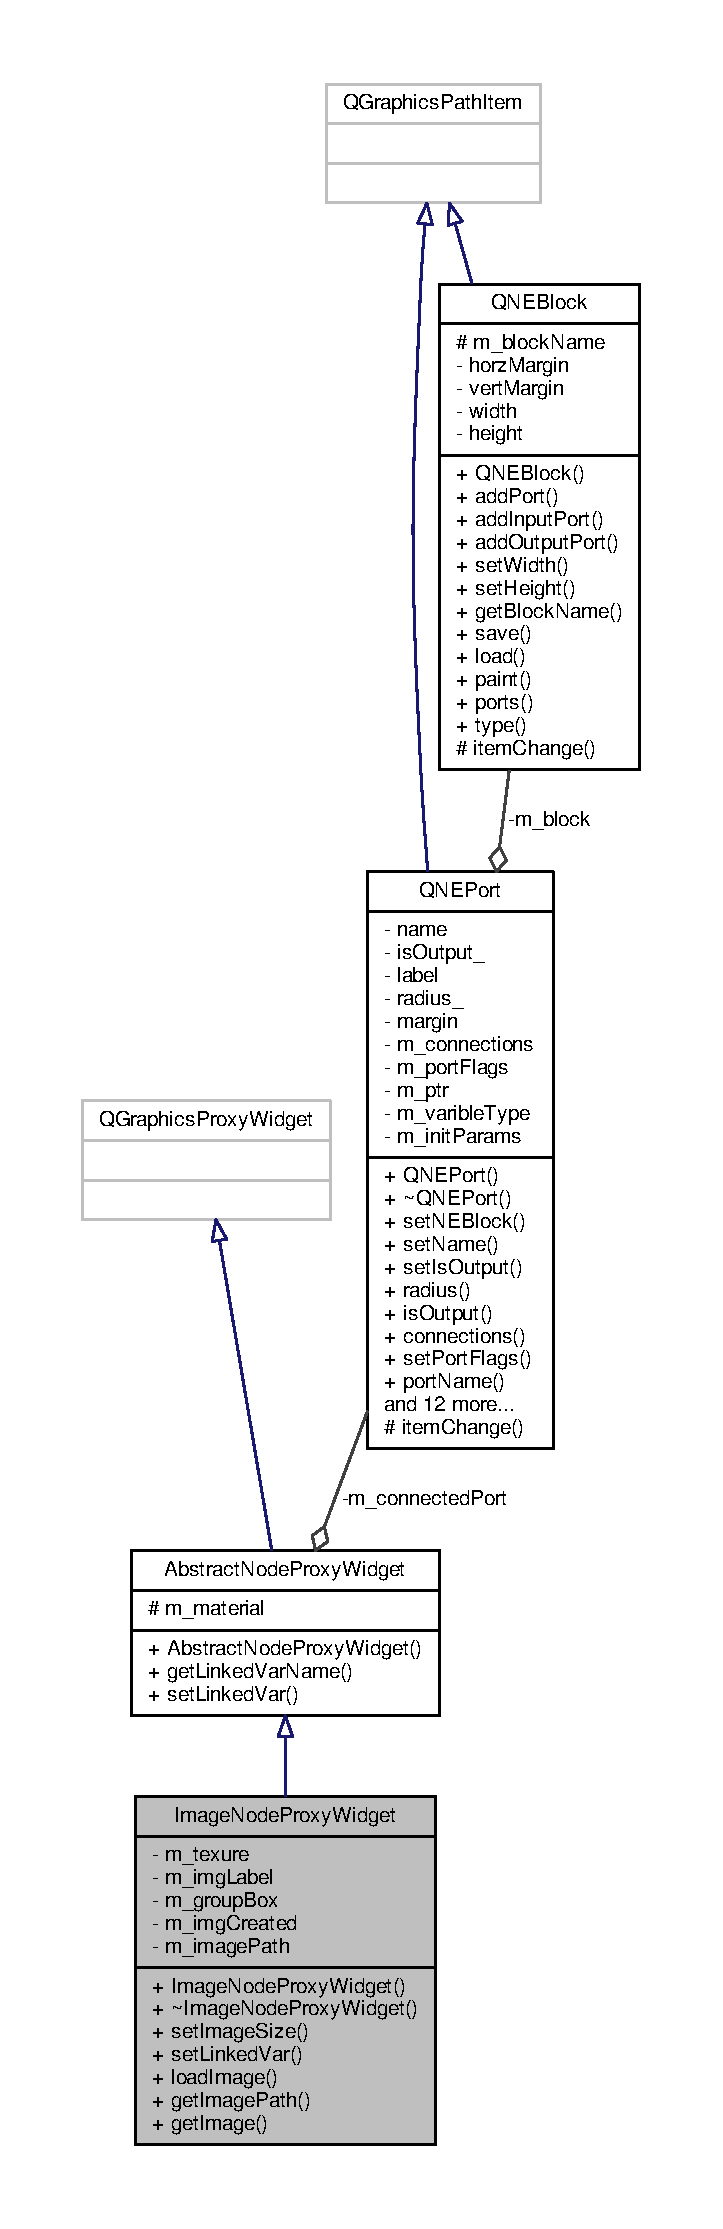
\includegraphics[height=550pt]{class_image_node_proxy_widget__coll__graph}
\end{center}
\end{figure}
\subsection*{Public Slots}
\begin{DoxyCompactItemize}
\item 
\hypertarget{class_image_node_proxy_widget_afb9272f0af02e0d8b5d70f2b7eb246eb}{void \hyperlink{class_image_node_proxy_widget_afb9272f0af02e0d8b5d70f2b7eb246eb}{get\-Image} ()}\label{class_image_node_proxy_widget_afb9272f0af02e0d8b5d70f2b7eb246eb}

\begin{DoxyCompactList}\small\item\em slot to import an image to our node \end{DoxyCompactList}\end{DoxyCompactItemize}
\subsection*{Public Member Functions}
\begin{DoxyCompactItemize}
\item 
\hypertarget{class_image_node_proxy_widget_aa978f88ffefe88664d6d4f5177224015}{{\bfseries Image\-Node\-Proxy\-Widget} (\hyperlink{class_q_n_e_port}{Q\-N\-E\-Port} $\ast$\-\_\-port\-Connected, optix\-::\-Material \&\-\_\-mat, Q\-Graphics\-Item $\ast$parent=0)}\label{class_image_node_proxy_widget_aa978f88ffefe88664d6d4f5177224015}

\item 
\hypertarget{class_image_node_proxy_widget_acbe422d61639eb6479ae01e2f4c6531a}{\hyperlink{class_image_node_proxy_widget_acbe422d61639eb6479ae01e2f4c6531a}{$\sim$\-Image\-Node\-Proxy\-Widget} ()}\label{class_image_node_proxy_widget_acbe422d61639eb6479ae01e2f4c6531a}

\begin{DoxyCompactList}\small\item\em default destructor \end{DoxyCompactList}\item 
\hypertarget{class_image_node_proxy_widget_af837a3a6278f17d6be03f309302d1614}{void \hyperlink{class_image_node_proxy_widget_af837a3a6278f17d6be03f309302d1614}{set\-Image\-Size} (int \-\_\-width, int \-\_\-height)}\label{class_image_node_proxy_widget_af837a3a6278f17d6be03f309302d1614}

\begin{DoxyCompactList}\small\item\em mutator to the width and height of our image \end{DoxyCompactList}\item 
\hypertarget{class_image_node_proxy_widget_a18574265844e2a6165ab6608f08a5fe1}{void \hyperlink{class_image_node_proxy_widget_a18574265844e2a6165ab6608f08a5fe1}{set\-Linked\-Var} ()}\label{class_image_node_proxy_widget_a18574265844e2a6165ab6608f08a5fe1}

\begin{DoxyCompactList}\small\item\em overite our set\-Linked\-Var function to put our own functionality in \end{DoxyCompactList}\item 
void \hyperlink{class_image_node_proxy_widget_a0930cf7ae23b7056c46f8ecd510f1542}{load\-Image} (Q\-String \-\_\-path)
\begin{DoxyCompactList}\small\item\em load an image into our widget \end{DoxyCompactList}\item 
\hypertarget{class_image_node_proxy_widget_a6e21c3e4552dc8a7da308a905c9b841d}{Q\-String \hyperlink{class_image_node_proxy_widget_a6e21c3e4552dc8a7da308a905c9b841d}{get\-Image\-Path} ()}\label{class_image_node_proxy_widget_a6e21c3e4552dc8a7da308a905c9b841d}

\begin{DoxyCompactList}\small\item\em accessor to image path \end{DoxyCompactList}\end{DoxyCompactItemize}
\subsection*{Private Attributes}
\begin{DoxyCompactItemize}
\item 
\hypertarget{class_image_node_proxy_widget_a6addc0eef24e9bc9b010eca29c126943}{optix\-::\-Texture\-Sampler \hyperlink{class_image_node_proxy_widget_a6addc0eef24e9bc9b010eca29c126943}{m\-\_\-texure}}\label{class_image_node_proxy_widget_a6addc0eef24e9bc9b010eca29c126943}

\begin{DoxyCompactList}\small\item\em our optix texture \end{DoxyCompactList}\item 
\hypertarget{class_image_node_proxy_widget_aede65813ea9649a733fb03226082fc54}{Q\-Label $\ast$ \hyperlink{class_image_node_proxy_widget_aede65813ea9649a733fb03226082fc54}{m\-\_\-img\-Label}}\label{class_image_node_proxy_widget_aede65813ea9649a733fb03226082fc54}

\begin{DoxyCompactList}\small\item\em label widget to hold our image \end{DoxyCompactList}\item 
\hypertarget{class_image_node_proxy_widget_a2bbc7434a8db9f8e49937968fcc1e5fe}{Q\-Group\-Box $\ast$ \hyperlink{class_image_node_proxy_widget_a2bbc7434a8db9f8e49937968fcc1e5fe}{m\-\_\-group\-Box}}\label{class_image_node_proxy_widget_a2bbc7434a8db9f8e49937968fcc1e5fe}

\begin{DoxyCompactList}\small\item\em our group box \end{DoxyCompactList}\item 
\hypertarget{class_image_node_proxy_widget_a6db30ded674d54f7b39fa5c4ffb5af26}{bool \hyperlink{class_image_node_proxy_widget_a6db30ded674d54f7b39fa5c4ffb5af26}{m\-\_\-img\-Created}}\label{class_image_node_proxy_widget_a6db30ded674d54f7b39fa5c4ffb5af26}

\begin{DoxyCompactList}\small\item\em bool to indicate if we have a texture created \end{DoxyCompactList}\item 
\hypertarget{class_image_node_proxy_widget_a90f807adc849eea5050763eb6a849f4e}{Q\-String \hyperlink{class_image_node_proxy_widget_a90f807adc849eea5050763eb6a849f4e}{m\-\_\-image\-Path}}\label{class_image_node_proxy_widget_a90f807adc849eea5050763eb6a849f4e}

\begin{DoxyCompactList}\small\item\em the image path \end{DoxyCompactList}\end{DoxyCompactItemize}
\subsection*{Additional Inherited Members}


\subsection{Detailed Description}
Extention of \hyperlink{class_abstract_node_proxy_widget}{Abstract\-Node\-Proxy\-Widget} that allows us to select an image and apply it to a attribute of a material. 

This Widget consists of a button to load in an image and a label to display the image. \begin{DoxyAuthor}{Author}
Declan Russell 
\end{DoxyAuthor}
\begin{DoxyDate}{Date}
05/05/2015 
\end{DoxyDate}


\subsection{Member Function Documentation}
\hypertarget{class_image_node_proxy_widget_a0930cf7ae23b7056c46f8ecd510f1542}{\index{Image\-Node\-Proxy\-Widget@{Image\-Node\-Proxy\-Widget}!load\-Image@{load\-Image}}
\index{load\-Image@{load\-Image}!ImageNodeProxyWidget@{Image\-Node\-Proxy\-Widget}}
\subsubsection[{load\-Image}]{\setlength{\rightskip}{0pt plus 5cm}void Image\-Node\-Proxy\-Widget\-::load\-Image (
\begin{DoxyParamCaption}
\item[{Q\-String}]{\-\_\-path}
\end{DoxyParamCaption}
)}}\label{class_image_node_proxy_widget_a0930cf7ae23b7056c46f8ecd510f1542}


load an image into our widget 


\begin{DoxyParams}{Parameters}
{\em \-\_\-path} & -\/ path to desired image \\
\hline
\end{DoxyParams}


Here is the call graph for this function\-:
\nopagebreak
\begin{figure}[H]
\begin{center}
\leavevmode
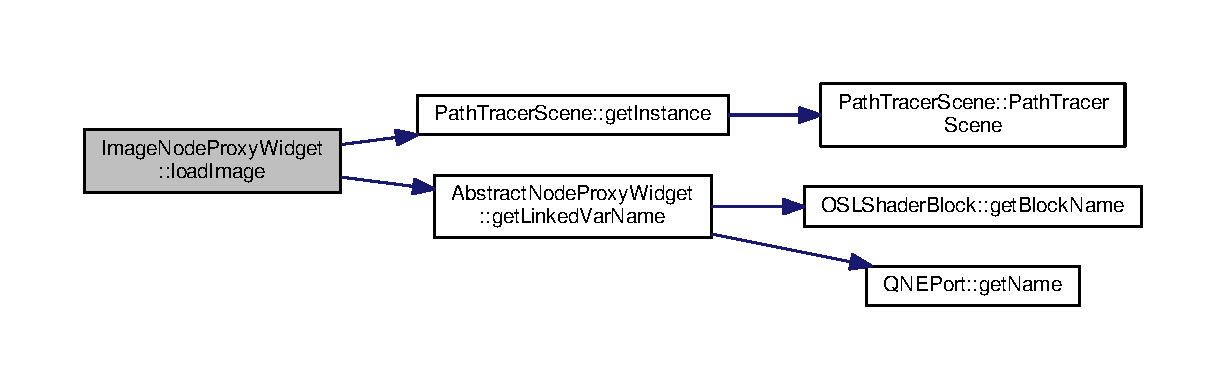
\includegraphics[width=350pt]{class_image_node_proxy_widget_a0930cf7ae23b7056c46f8ecd510f1542_cgraph}
\end{center}
\end{figure}




Here is the caller graph for this function\-:
\nopagebreak
\begin{figure}[H]
\begin{center}
\leavevmode
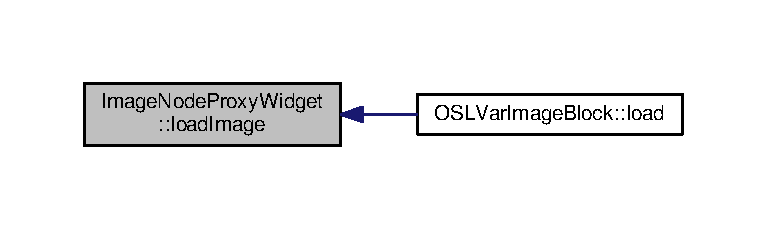
\includegraphics[width=350pt]{class_image_node_proxy_widget_a0930cf7ae23b7056c46f8ecd510f1542_icgraph}
\end{center}
\end{figure}




The documentation for this class was generated from the following files\-:\begin{DoxyCompactItemize}
\item 
include/\-Node\-Graph/Image\-Node\-Proxy\-Widget.\-h\item 
src/\-Node\-Graph/Image\-Node\-Proxy\-Widget.\-cpp\end{DoxyCompactItemize}

\hypertarget{struct_instruction}{\section{Instruction Struct Reference}
\label{struct_instruction}\index{Instruction@{Instruction}}
}


An instruction within the O\-S\-O code section.  




{\ttfamily \#include $<$Oso\-Reader.\-h$>$}



Collaboration diagram for Instruction\-:
\nopagebreak
\begin{figure}[H]
\begin{center}
\leavevmode
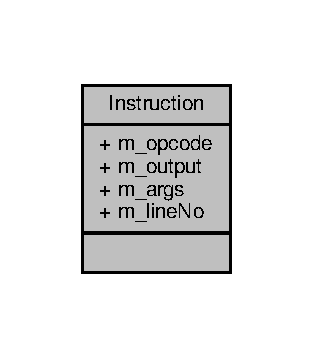
\includegraphics[width=150pt]{struct_instruction__coll__graph}
\end{center}
\end{figure}
\subsection*{Public Attributes}
\begin{DoxyCompactItemize}
\item 
\hypertarget{struct_instruction_aee4a8374afe12c8a7edbebd5b59adec1}{std\-::string {\bfseries m\-\_\-opcode} = std\-::string(\char`\"{}void\char`\"{})}\label{struct_instruction_aee4a8374afe12c8a7edbebd5b59adec1}

\item 
\hypertarget{struct_instruction_a02ef9c6ba83385398b4d303ba8ff72af}{std\-::string {\bfseries m\-\_\-output} = std\-::string(\char`\"{}void\char`\"{})}\label{struct_instruction_a02ef9c6ba83385398b4d303ba8ff72af}

\item 
\hypertarget{struct_instruction_afe73084538ea1cbbd9df65ab431e879d}{std\-::vector$<$ std\-::string $>$ {\bfseries m\-\_\-args}}\label{struct_instruction_afe73084538ea1cbbd9df65ab431e879d}

\item 
\hypertarget{struct_instruction_af01a80e058a81bf60a863de8d7684aec}{int {\bfseries m\-\_\-line\-No}}\label{struct_instruction_af01a80e058a81bf60a863de8d7684aec}

\end{DoxyCompactItemize}


\subsection{Detailed Description}
An instruction within the O\-S\-O code section. 

The documentation for this struct was generated from the following file\-:\begin{DoxyCompactItemize}
\item 
include/\-O\-S\-L\-Compiler/Oso\-Reader.\-h\end{DoxyCompactItemize}

\hypertarget{class_int_node_proxy_widget}{\section{Int\-Node\-Proxy\-Widget Class Reference}
\label{class_int_node_proxy_widget}\index{Int\-Node\-Proxy\-Widget@{Int\-Node\-Proxy\-Widget}}
}


Extention of \hyperlink{class_abstract_node_proxy_widget}{Abstract\-Node\-Proxy\-Widget} that allows us to select an int and apply it to a attribute of a material.  




{\ttfamily \#include $<$Int\-Node\-Proxy\-Widget.\-h$>$}



Inheritance diagram for Int\-Node\-Proxy\-Widget\-:
\nopagebreak
\begin{figure}[H]
\begin{center}
\leavevmode
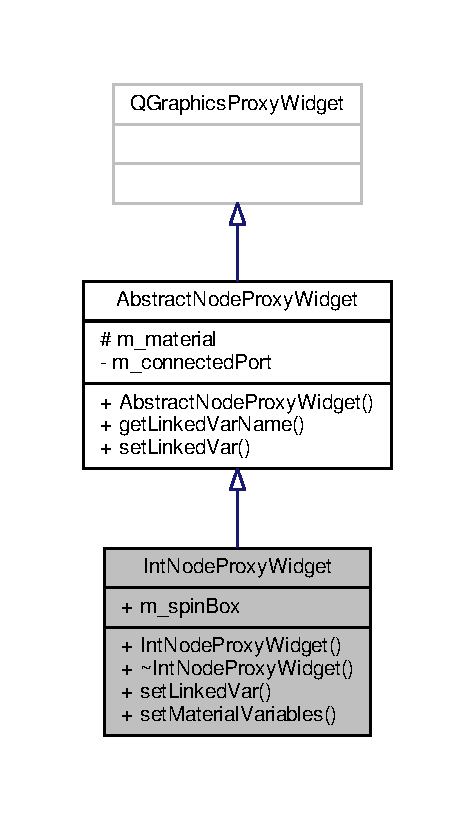
\includegraphics[width=228pt]{class_int_node_proxy_widget__inherit__graph}
\end{center}
\end{figure}


Collaboration diagram for Int\-Node\-Proxy\-Widget\-:
\nopagebreak
\begin{figure}[H]
\begin{center}
\leavevmode
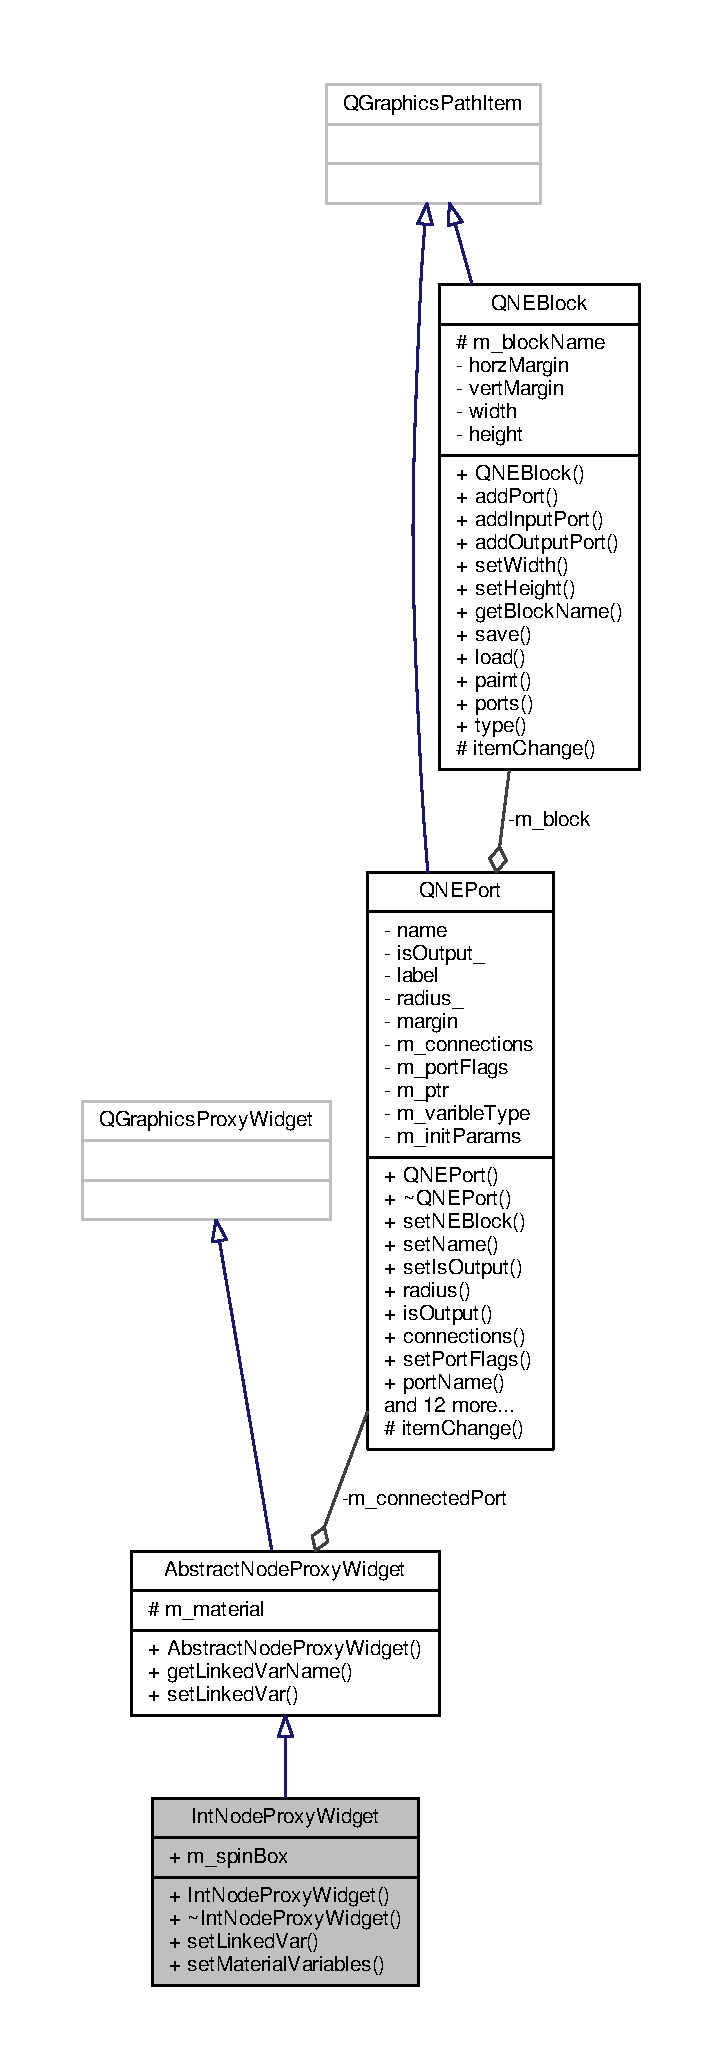
\includegraphics[height=550pt]{class_int_node_proxy_widget__coll__graph}
\end{center}
\end{figure}
\subsection*{Public Slots}
\begin{DoxyCompactItemize}
\item 
void \hyperlink{class_int_node_proxy_widget_a04d972bdd37258011454c1fc116723cd}{set\-Material\-Variables} (int \-\_\-val)
\begin{DoxyCompactList}\small\item\em slot to set the varible in our material when our spin box value is changed \end{DoxyCompactList}\end{DoxyCompactItemize}
\subsection*{Public Member Functions}
\begin{DoxyCompactItemize}
\item 
\hypertarget{class_int_node_proxy_widget_a94ec15988e7cc2f2c569ba380aba142d}{{\bfseries Int\-Node\-Proxy\-Widget} (\hyperlink{class_q_n_e_port}{Q\-N\-E\-Port} $\ast$\-\_\-port\-Connected, optix\-::\-Material \&\-\_\-mat, Q\-Graphics\-Item $\ast$parent=0)}\label{class_int_node_proxy_widget_a94ec15988e7cc2f2c569ba380aba142d}

\item 
\hypertarget{class_int_node_proxy_widget_a04f883865fdd60c96084b3dbb61f4051}{\hyperlink{class_int_node_proxy_widget_a04f883865fdd60c96084b3dbb61f4051}{$\sim$\-Int\-Node\-Proxy\-Widget} ()}\label{class_int_node_proxy_widget_a04f883865fdd60c96084b3dbb61f4051}

\begin{DoxyCompactList}\small\item\em default destructor \end{DoxyCompactList}\item 
\hypertarget{class_int_node_proxy_widget_a36821d35f9e61bf34e504c2c6d980388}{void \hyperlink{class_int_node_proxy_widget_a36821d35f9e61bf34e504c2c6d980388}{set\-Linked\-Var} ()}\label{class_int_node_proxy_widget_a36821d35f9e61bf34e504c2c6d980388}

\begin{DoxyCompactList}\small\item\em overite our set\-Linked\-Var function to put our own functionality in \end{DoxyCompactList}\end{DoxyCompactItemize}
\subsection*{Public Attributes}
\begin{DoxyCompactItemize}
\item 
\hypertarget{class_int_node_proxy_widget_aedc2e466a1407c2b3be36e7895b81c5d}{Q\-Spin\-Box $\ast$ \hyperlink{class_int_node_proxy_widget_aedc2e466a1407c2b3be36e7895b81c5d}{m\-\_\-spin\-Box}}\label{class_int_node_proxy_widget_aedc2e466a1407c2b3be36e7895b81c5d}

\begin{DoxyCompactList}\small\item\em a member for our spin box \end{DoxyCompactList}\end{DoxyCompactItemize}
\subsection*{Additional Inherited Members}


\subsection{Detailed Description}
Extention of \hyperlink{class_abstract_node_proxy_widget}{Abstract\-Node\-Proxy\-Widget} that allows us to select an int and apply it to a attribute of a material. 

This widget consists of a single Spin\-Box to select a integer value. \begin{DoxyAuthor}{Author}
Declan Russell 
\end{DoxyAuthor}
\begin{DoxyDate}{Date}
05/05/2015 
\end{DoxyDate}


\subsection{Member Function Documentation}
\hypertarget{class_int_node_proxy_widget_a04d972bdd37258011454c1fc116723cd}{\index{Int\-Node\-Proxy\-Widget@{Int\-Node\-Proxy\-Widget}!set\-Material\-Variables@{set\-Material\-Variables}}
\index{set\-Material\-Variables@{set\-Material\-Variables}!IntNodeProxyWidget@{Int\-Node\-Proxy\-Widget}}
\subsubsection[{set\-Material\-Variables}]{\setlength{\rightskip}{0pt plus 5cm}void Int\-Node\-Proxy\-Widget\-::set\-Material\-Variables (
\begin{DoxyParamCaption}
\item[{int}]{\-\_\-val}
\end{DoxyParamCaption}
)\hspace{0.3cm}{\ttfamily [slot]}}}\label{class_int_node_proxy_widget_a04d972bdd37258011454c1fc116723cd}


slot to set the varible in our material when our spin box value is changed 


\begin{DoxyParams}{Parameters}
{\em \-\_\-val} & the value to set the variables in our material \\
\hline
\end{DoxyParams}


Here is the call graph for this function\-:
\nopagebreak
\begin{figure}[H]
\begin{center}
\leavevmode
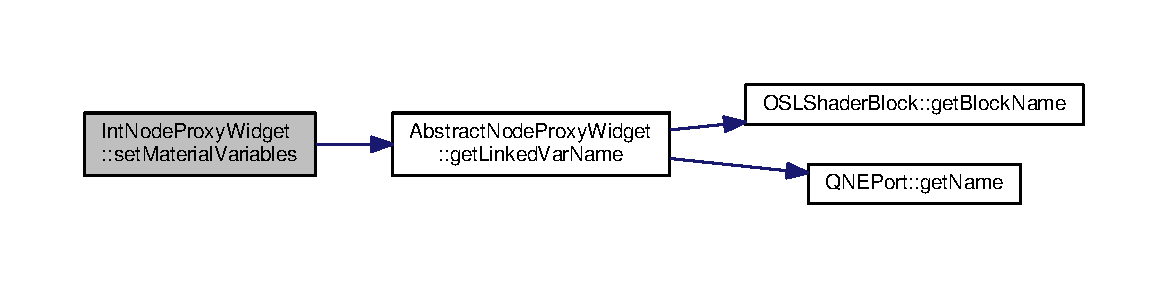
\includegraphics[width=350pt]{class_int_node_proxy_widget_a04d972bdd37258011454c1fc116723cd_cgraph}
\end{center}
\end{figure}




The documentation for this class was generated from the following files\-:\begin{DoxyCompactItemize}
\item 
include/\-Node\-Graph/Int\-Node\-Proxy\-Widget.\-h\item 
src/\-Node\-Graph/Int\-Node\-Proxy\-Widget.\-cpp\end{DoxyCompactItemize}

\hypertarget{struct_jump_target}{\section{Jump\-Target Struct Reference}
\label{struct_jump_target}\index{Jump\-Target@{Jump\-Target}}
}


A structure to hold jump targets for use will if/else statements.  




{\ttfamily \#include $<$Oso\-Reader.\-h$>$}



Collaboration diagram for Jump\-Target\-:
\nopagebreak
\begin{figure}[H]
\begin{center}
\leavevmode
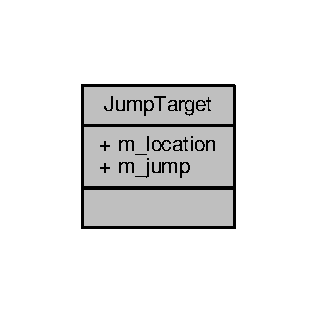
\includegraphics[width=152pt]{struct_jump_target__coll__graph}
\end{center}
\end{figure}
\subsection*{Public Attributes}
\begin{DoxyCompactItemize}
\item 
\hypertarget{struct_jump_target_a96654265b4443a164bd74cdddf7fbb70}{int {\bfseries m\-\_\-location}}\label{struct_jump_target_a96654265b4443a164bd74cdddf7fbb70}

\item 
\hypertarget{struct_jump_target_aac06f4a996acfb8e891735b94538efe4}{int {\bfseries m\-\_\-jump}}\label{struct_jump_target_aac06f4a996acfb8e891735b94538efe4}

\end{DoxyCompactItemize}


\subsection{Detailed Description}
A structure to hold jump targets for use will if/else statements. 

The documentation for this struct was generated from the following file\-:\begin{DoxyCompactItemize}
\item 
include/\-O\-S\-L\-Compiler/Oso\-Reader.\-h\end{DoxyCompactItemize}

\hypertarget{class_light}{\section{Light Class Reference}
\label{class_light}\index{Light@{Light}}
}


Collaboration diagram for Light\-:
\nopagebreak
\begin{figure}[H]
\begin{center}
\leavevmode
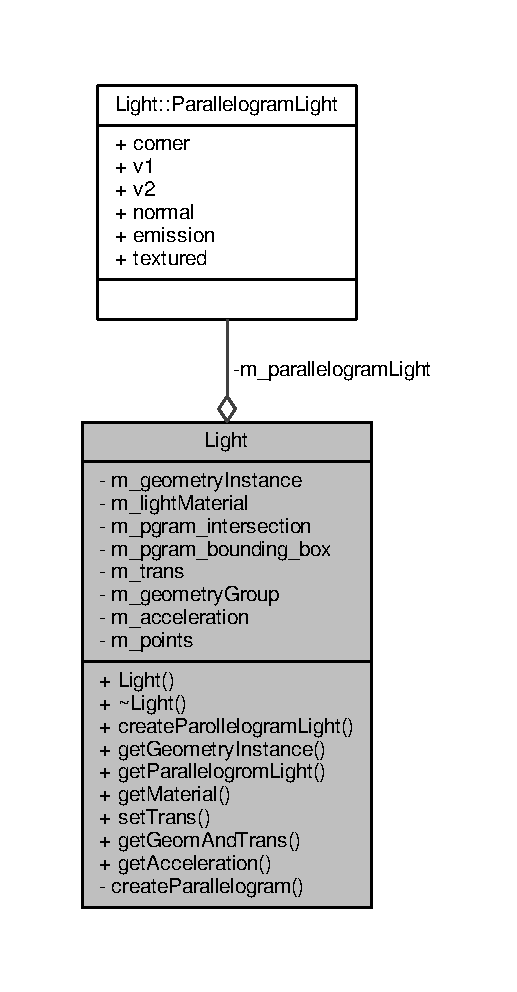
\includegraphics[width=248pt]{class_light__coll__graph}
\end{center}
\end{figure}
\subsection*{Classes}
\begin{DoxyCompactItemize}
\item 
struct \hyperlink{struct_light_1_1_parallelogram_light}{Parallelogram\-Light}
\begin{DoxyCompactList}\small\item\em A structure to hold information about our parallelogram area lights. \end{DoxyCompactList}\end{DoxyCompactItemize}
\subsection*{Public Member Functions}
\begin{DoxyCompactItemize}
\item 
\hypertarget{class_light_aeb5df09a25a32f19fdffa761268ba24f}{\hyperlink{class_light_aeb5df09a25a32f19fdffa761268ba24f}{Light} ()}\label{class_light_aeb5df09a25a32f19fdffa761268ba24f}

\begin{DoxyCompactList}\small\item\em Constructor. \end{DoxyCompactList}\item 
\hypertarget{class_light_ad0e59fad13bb6cfadc25b2c477e9ddc7}{\hyperlink{class_light_ad0e59fad13bb6cfadc25b2c477e9ddc7}{$\sim$\-Light} ()}\label{class_light_ad0e59fad13bb6cfadc25b2c477e9ddc7}

\begin{DoxyCompactList}\small\item\em Destructor. \end{DoxyCompactList}\item 
\hypertarget{class_light_a7621ee283ddbe3fec59dee5c34e6317a}{void \hyperlink{class_light_a7621ee283ddbe3fec59dee5c34e6317a}{create\-Parollelogram\-Light} ()}\label{class_light_a7621ee283ddbe3fec59dee5c34e6317a}

\begin{DoxyCompactList}\small\item\em Create a parallelogram shaped light. \end{DoxyCompactList}\item 
\hypertarget{class_light_accfd9bb583a936a092bcca37866f0f40}{optix\-::\-Geometry\-Instance \hyperlink{class_light_accfd9bb583a936a092bcca37866f0f40}{get\-Geometry\-Instance} ()}\label{class_light_accfd9bb583a936a092bcca37866f0f40}

\begin{DoxyCompactList}\small\item\em Returns the gemoetry instance for the light. \end{DoxyCompactList}\item 
\hypertarget{class_light_a4a50c1f55863d0e7bcb6e15c56161f89}{\hyperlink{struct_light_1_1_parallelogram_light}{Parallelogram\-Light} \hyperlink{class_light_a4a50c1f55863d0e7bcb6e15c56161f89}{get\-Parallelogrom\-Light} ()}\label{class_light_a4a50c1f55863d0e7bcb6e15c56161f89}

\begin{DoxyCompactList}\small\item\em Returns the Parallelogram data structure for holding the light information. \end{DoxyCompactList}\item 
\hypertarget{class_light_a56ae6197fefbc72b1114a696539d9e41}{optix\-::\-Material \hyperlink{class_light_a56ae6197fefbc72b1114a696539d9e41}{get\-Material} ()}\label{class_light_a56ae6197fefbc72b1114a696539d9e41}

\begin{DoxyCompactList}\small\item\em Returns the material attached to the light. \end{DoxyCompactList}\item 
\hypertarget{class_light_a547b5f6bce87bb1afaa310da7e60debd}{void {\bfseries set\-Trans} (glm\-::mat4 \-\_\-trans, bool \-\_\-transpose=0)}\label{class_light_a547b5f6bce87bb1afaa310da7e60debd}

\item 
\hypertarget{class_light_a40b9f2558fab3ad3368eeda329dcd540}{optix\-::\-Transform {\bfseries get\-Geom\-And\-Trans} ()}\label{class_light_a40b9f2558fab3ad3368eeda329dcd540}

\item 
\hypertarget{class_light_aa3dc480efad5296465c3221a0ae5ccb3}{optix\-::\-Acceleration {\bfseries get\-Acceleration} ()}\label{class_light_aa3dc480efad5296465c3221a0ae5ccb3}

\end{DoxyCompactItemize}
\subsection*{Private Member Functions}
\begin{DoxyCompactItemize}
\item 
\hypertarget{class_light_abcc5c13ce90a138c34cd2176414ca796}{optix\-::\-Geometry\-Instance \hyperlink{class_light_abcc5c13ce90a138c34cd2176414ca796}{create\-Parallelogram} (const optix\-::float3 \&\-\_\-point1, const optix\-::float3 \&\-\_\-point2, const optix\-::float3 \&\-\_\-point3)}\label{class_light_abcc5c13ce90a138c34cd2176414ca796}

\begin{DoxyCompactList}\small\item\em Create the parallelogram geometry used by the light. \end{DoxyCompactList}\end{DoxyCompactItemize}
\subsection*{Private Attributes}
\begin{DoxyCompactItemize}
\item 
\hypertarget{class_light_a1a38877bc851fc52aa56b74797cd4b39}{optix\-::\-Geometry\-Instance \hyperlink{class_light_a1a38877bc851fc52aa56b74797cd4b39}{m\-\_\-geometry\-Instance}}\label{class_light_a1a38877bc851fc52aa56b74797cd4b39}

\begin{DoxyCompactList}\small\item\em The geometry instance. \end{DoxyCompactList}\item 
\hypertarget{class_light_ae9a20c4be482422ffbfdbd20cbdced3b}{\hyperlink{struct_light_1_1_parallelogram_light}{Parallelogram\-Light} \hyperlink{class_light_ae9a20c4be482422ffbfdbd20cbdced3b}{m\-\_\-parallelogram\-Light}}\label{class_light_ae9a20c4be482422ffbfdbd20cbdced3b}

\begin{DoxyCompactList}\small\item\em The data structure for holding information about the light. \end{DoxyCompactList}\item 
\hypertarget{class_light_a717ad0883b7b5d662411ff8e07adc672}{optix\-::\-Material \hyperlink{class_light_a717ad0883b7b5d662411ff8e07adc672}{m\-\_\-light\-Material}}\label{class_light_a717ad0883b7b5d662411ff8e07adc672}

\begin{DoxyCompactList}\small\item\em The optix material attached to the light. \end{DoxyCompactList}\item 
\hypertarget{class_light_af3b4e7b6a3666c514b3d096529cf1f11}{optix\-::\-Program \hyperlink{class_light_af3b4e7b6a3666c514b3d096529cf1f11}{m\-\_\-pgram\-\_\-intersection}}\label{class_light_af3b4e7b6a3666c514b3d096529cf1f11}

\begin{DoxyCompactList}\small\item\em The intersection program used for the light geometry. \end{DoxyCompactList}\item 
\hypertarget{class_light_ab024a48ce987f83ea350b9ea5312a13a}{optix\-::\-Program \hyperlink{class_light_ab024a48ce987f83ea350b9ea5312a13a}{m\-\_\-pgram\-\_\-bounding\-\_\-box}}\label{class_light_ab024a48ce987f83ea350b9ea5312a13a}

\begin{DoxyCompactList}\small\item\em An A\-A\-B\-B intersection program for the light geometry. \end{DoxyCompactList}\item 
\hypertarget{class_light_a4f27233a6a4f24bd6af470325722e91f}{optix\-::\-Transform \hyperlink{class_light_a4f27233a6a4f24bd6af470325722e91f}{m\-\_\-trans}}\label{class_light_a4f27233a6a4f24bd6af470325722e91f}

\begin{DoxyCompactList}\small\item\em A translation. \end{DoxyCompactList}\item 
\hypertarget{class_light_a303ad623513cfe674f4a49096358d24e}{optix\-::\-Geometry\-Group {\bfseries m\-\_\-geometry\-Group}}\label{class_light_a303ad623513cfe674f4a49096358d24e}

\item 
\hypertarget{class_light_a4bf35bc5c66a467228b76098a8775c5c}{optix\-::\-Acceleration {\bfseries m\-\_\-acceleration}}\label{class_light_a4bf35bc5c66a467228b76098a8775c5c}

\item 
\hypertarget{class_light_a6f7c0af5a0fec1b1a8a941e14943f006}{float {\bfseries m\-\_\-points} \mbox{[}4\mbox{]}}\label{class_light_a6f7c0af5a0fec1b1a8a941e14943f006}

\end{DoxyCompactItemize}


The documentation for this class was generated from the following files\-:\begin{DoxyCompactItemize}
\item 
include/\-Lights/Light.\-h\item 
src/\-Lights/Light.\-cpp\end{DoxyCompactItemize}

\hypertarget{structlight_info}{\section{light\-Info Struct Reference}
\label{structlight_info}\index{light\-Info@{light\-Info}}
}


Collaboration diagram for light\-Info\-:
\nopagebreak
\begin{figure}[H]
\begin{center}
\leavevmode
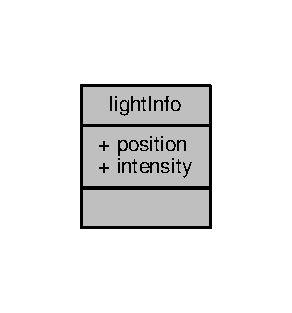
\includegraphics[width=140pt]{structlight_info__coll__graph}
\end{center}
\end{figure}
\subsection*{Public Attributes}
\begin{DoxyCompactItemize}
\item 
\hypertarget{structlight_info_a91464db499bb017224ed4137db3ad357}{vec4 {\bfseries position}}\label{structlight_info_a91464db499bb017224ed4137db3ad357}

\item 
\hypertarget{structlight_info_a0a3a282dd8998aed665222fd1902611f}{vec3 {\bfseries intensity}}\label{structlight_info_a0a3a282dd8998aed665222fd1902611f}

\end{DoxyCompactItemize}


The documentation for this struct was generated from the following file\-:\begin{DoxyCompactItemize}
\item 
shaders/Phong\-Frag.\-glsl\end{DoxyCompactItemize}

\hypertarget{class_light_manager}{\section{Light\-Manager Class Reference}
\label{class_light_manager}\index{Light\-Manager@{Light\-Manager}}
}


Inheritance diagram for Light\-Manager\-:
\nopagebreak
\begin{figure}[H]
\begin{center}
\leavevmode
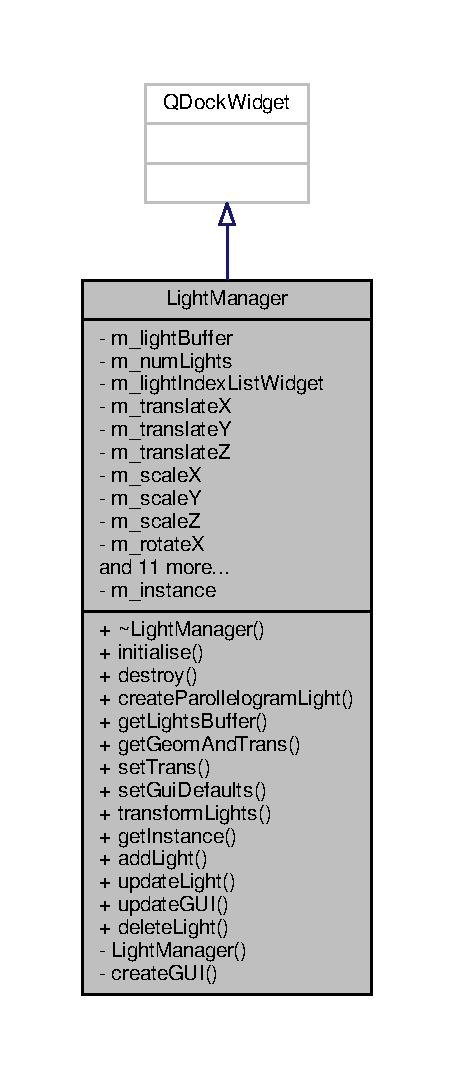
\includegraphics[width=218pt]{class_light_manager__inherit__graph}
\end{center}
\end{figure}


Collaboration diagram for Light\-Manager\-:
\nopagebreak
\begin{figure}[H]
\begin{center}
\leavevmode
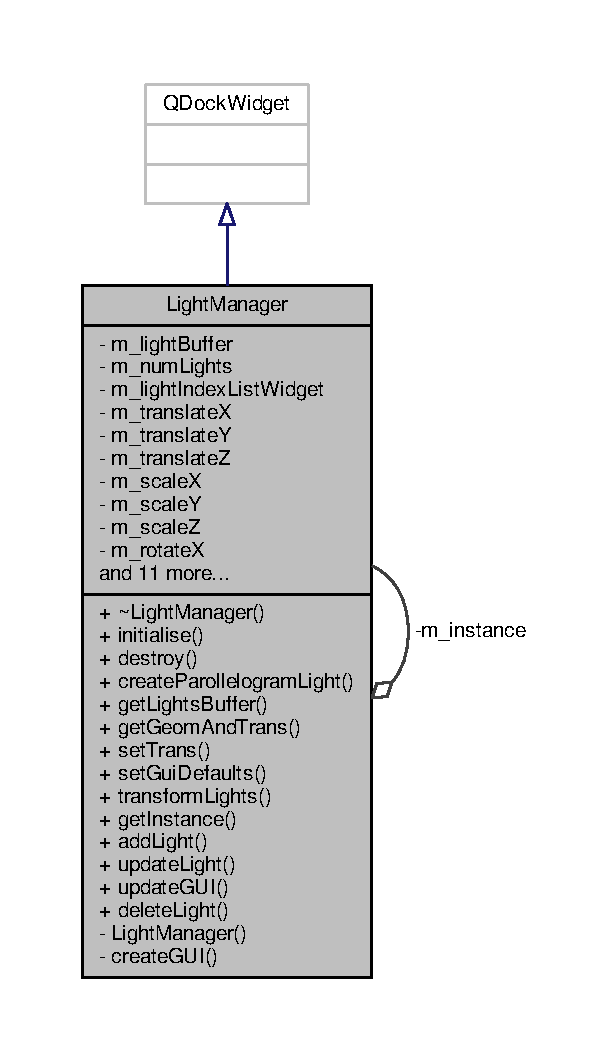
\includegraphics[width=293pt]{class_light_manager__coll__graph}
\end{center}
\end{figure}
\subsection*{Classes}
\begin{DoxyCompactItemize}
\item 
struct \hyperlink{struct_light_manager_1_1_light_transforms}{Light\-Transforms}
\end{DoxyCompactItemize}
\subsection*{Public Slots}
\begin{DoxyCompactItemize}
\item 
\hypertarget{class_light_manager_aa25de876fdf8e06b33e6d8e161f8a44e}{void \hyperlink{class_light_manager_aa25de876fdf8e06b33e6d8e161f8a44e}{add\-Light} ()}\label{class_light_manager_aa25de876fdf8e06b33e6d8e161f8a44e}

\begin{DoxyCompactList}\small\item\em Adds a light to the scene. \end{DoxyCompactList}\item 
\hypertarget{class_light_manager_a403f28b82c78e0b9946848f16ecd7581}{void \hyperlink{class_light_manager_a403f28b82c78e0b9946848f16ecd7581}{update\-Light} ()}\label{class_light_manager_a403f28b82c78e0b9946848f16ecd7581}

\begin{DoxyCompactList}\small\item\em Update a light already created. \end{DoxyCompactList}\item 
\hypertarget{class_light_manager_ad50e75aa287fa5c623fef70c820de9b6}{void \hyperlink{class_light_manager_ad50e75aa287fa5c623fef70c820de9b6}{update\-G\-U\-I} (Q\-Model\-Index \-\_\-index)}\label{class_light_manager_ad50e75aa287fa5c623fef70c820de9b6}

\begin{DoxyCompactList}\small\item\em Update the gui for the current light selected. \end{DoxyCompactList}\item 
\hypertarget{class_light_manager_a277063837cd2e2d17fd1e221e39add4a}{void \hyperlink{class_light_manager_a277063837cd2e2d17fd1e221e39add4a}{delete\-Light} ()}\label{class_light_manager_a277063837cd2e2d17fd1e221e39add4a}

\begin{DoxyCompactList}\small\item\em Deletes a light from the scene. \end{DoxyCompactList}\end{DoxyCompactItemize}
\subsection*{Signals}
\begin{DoxyCompactItemize}
\item 
\hypertarget{class_light_manager_a8292d4fd581eb7f72c68976732f5fa3b}{void {\bfseries update\-Scene} ()}\label{class_light_manager_a8292d4fd581eb7f72c68976732f5fa3b}

\end{DoxyCompactItemize}
\subsection*{Public Member Functions}
\begin{DoxyCompactItemize}
\item 
\hypertarget{class_light_manager_a07c7063f02e20a33c0984965991aa4af}{\hyperlink{class_light_manager_a07c7063f02e20a33c0984965991aa4af}{$\sim$\-Light\-Manager} ()}\label{class_light_manager_a07c7063f02e20a33c0984965991aa4af}

\begin{DoxyCompactList}\small\item\em Destructor. \end{DoxyCompactList}\item 
\hypertarget{class_light_manager_ae415dd0ef2294e649b546d928837b860}{void \hyperlink{class_light_manager_ae415dd0ef2294e649b546d928837b860}{initialise} ()}\label{class_light_manager_ae415dd0ef2294e649b546d928837b860}

\begin{DoxyCompactList}\small\item\em Initialise the light buffer. \end{DoxyCompactList}\item 
\hypertarget{class_light_manager_ae54246d612d778d892d6473a43a83d32}{void \hyperlink{class_light_manager_ae54246d612d778d892d6473a43a83d32}{destroy} ()}\label{class_light_manager_ae54246d612d778d892d6473a43a83d32}

\begin{DoxyCompactList}\small\item\em destroys our singleton class \end{DoxyCompactList}\item 
\hypertarget{class_light_manager_a714fcbcf37902d8bd0e0b5676d00e121}{void \hyperlink{class_light_manager_a714fcbcf37902d8bd0e0b5676d00e121}{create\-Parollelogram\-Light} ()}\label{class_light_manager_a714fcbcf37902d8bd0e0b5676d00e121}

\begin{DoxyCompactList}\small\item\em Create a new parallelogram light. \end{DoxyCompactList}\item 
\hypertarget{class_light_manager_ad265f49547aeb715f2b33642a7a22fe6}{optix\-::\-Buffer \hyperlink{class_light_manager_ad265f49547aeb715f2b33642a7a22fe6}{get\-Lights\-Buffer} ()}\label{class_light_manager_ad265f49547aeb715f2b33642a7a22fe6}

\begin{DoxyCompactList}\small\item\em Returns our optix buffer containing information about our lights. \end{DoxyCompactList}\item 
\hypertarget{class_light_manager_a1c67bccf06073356ab849c42a6cc9c36}{std\-::vector$<$ optix\-::\-Transform $>$ \hyperlink{class_light_manager_a1c67bccf06073356ab849c42a6cc9c36}{get\-Geom\-And\-Trans} ()}\label{class_light_manager_a1c67bccf06073356ab849c42a6cc9c36}

\begin{DoxyCompactList}\small\item\em Returns the transform node for attaching to the scene graph. \end{DoxyCompactList}\item 
\hypertarget{class_light_manager_ae22469b57f40bd5b7d21ac6d857f8ce6}{void \hyperlink{class_light_manager_ae22469b57f40bd5b7d21ac6d857f8ce6}{set\-Trans} (optix\-::\-Transform \-\_\-transform, glm\-::mat4 \-\_\-trans, bool \-\_\-transpose=0)}\label{class_light_manager_ae22469b57f40bd5b7d21ac6d857f8ce6}

\begin{DoxyCompactList}\small\item\em Used for translating lights. \end{DoxyCompactList}\item 
\hypertarget{class_light_manager_acef6714d411c825fc6599a1c892fc9ff}{void \hyperlink{class_light_manager_acef6714d411c825fc6599a1c892fc9ff}{set\-Gui\-Defaults} ()}\label{class_light_manager_acef6714d411c825fc6599a1c892fc9ff}

\begin{DoxyCompactList}\small\item\em Sets the G\-U\-I to the default values. \end{DoxyCompactList}\item 
\hypertarget{class_light_manager_a50a3c0743afffc6db604e5eb325968c2}{void \hyperlink{class_light_manager_a50a3c0743afffc6db604e5eb325968c2}{transform\-Lights} (glm\-::mat4 \-\_\-trans)}\label{class_light_manager_a50a3c0743afffc6db604e5eb325968c2}

\begin{DoxyCompactList}\small\item\em Transforms lights when scene camera moves. \end{DoxyCompactList}\end{DoxyCompactItemize}
\subsection*{Static Public Member Functions}
\begin{DoxyCompactItemize}
\item 
\hypertarget{class_light_manager_a340b84ff20d73b644cbdab2f77eba5e6}{static \hyperlink{class_light_manager}{Light\-Manager} $\ast$ \hyperlink{class_light_manager_a340b84ff20d73b644cbdab2f77eba5e6}{get\-Instance} (Q\-Widget $\ast$parent=0)}\label{class_light_manager_a340b84ff20d73b644cbdab2f77eba5e6}

\begin{DoxyCompactList}\small\item\em returns an instance of our singleton class \end{DoxyCompactList}\end{DoxyCompactItemize}
\subsection*{Private Member Functions}
\begin{DoxyCompactItemize}
\item 
\hypertarget{class_light_manager_af7566c95a70bbf2b8fb03f9565dd4f2e}{\hyperlink{class_light_manager_af7566c95a70bbf2b8fb03f9565dd4f2e}{Light\-Manager} (Q\-Widget $\ast$parent=0)}\label{class_light_manager_af7566c95a70bbf2b8fb03f9565dd4f2e}

\begin{DoxyCompactList}\small\item\em Constructor. \end{DoxyCompactList}\item 
\hypertarget{class_light_manager_af36184ad28565d27b80f213ef8ac04a1}{void \hyperlink{class_light_manager_af36184ad28565d27b80f213ef8ac04a1}{create\-G\-U\-I} ()}\label{class_light_manager_af36184ad28565d27b80f213ef8ac04a1}

\begin{DoxyCompactList}\small\item\em Creates our G\-U\-I elements. \end{DoxyCompactList}\end{DoxyCompactItemize}
\subsection*{Private Attributes}
\begin{DoxyCompactItemize}
\item 
\hypertarget{class_light_manager_adf0c079124707803ea2e0a96b67eb68c}{optix\-::\-Buffer \hyperlink{class_light_manager_adf0c079124707803ea2e0a96b67eb68c}{m\-\_\-light\-Buffer}}\label{class_light_manager_adf0c079124707803ea2e0a96b67eb68c}

\begin{DoxyCompactList}\small\item\em A buffer to hold our lights. \end{DoxyCompactList}\item 
\hypertarget{class_light_manager_aba2dca016525dace316ce7c3b38f5f99}{unsigned int \hyperlink{class_light_manager_aba2dca016525dace316ce7c3b38f5f99}{m\-\_\-num\-Lights}}\label{class_light_manager_aba2dca016525dace316ce7c3b38f5f99}

\begin{DoxyCompactList}\small\item\em A variable to store the number of lights in our buffer. \end{DoxyCompactList}\item 
\hypertarget{class_light_manager_a5ac6ccaa5449249f75536df87c0709a9}{Q\-List\-Widget $\ast$ \hyperlink{class_light_manager_a5ac6ccaa5449249f75536df87c0709a9}{m\-\_\-light\-Index\-List\-Widget}}\label{class_light_manager_a5ac6ccaa5449249f75536df87c0709a9}

\begin{DoxyCompactList}\small\item\em A list to hold all our lights. \end{DoxyCompactList}\item 
\hypertarget{class_light_manager_a1d232847280fef0ad277c27bf7c2ec5e}{Q\-Double\-Spin\-Box $\ast$ \hyperlink{class_light_manager_a1d232847280fef0ad277c27bf7c2ec5e}{m\-\_\-translate\-X}}\label{class_light_manager_a1d232847280fef0ad277c27bf7c2ec5e}

\begin{DoxyCompactList}\small\item\em Our translation gui box for the x axis. \end{DoxyCompactList}\item 
\hypertarget{class_light_manager_a1129eb4551830ded49621b7a35638315}{Q\-Double\-Spin\-Box $\ast$ \hyperlink{class_light_manager_a1129eb4551830ded49621b7a35638315}{m\-\_\-translate\-Y}}\label{class_light_manager_a1129eb4551830ded49621b7a35638315}

\begin{DoxyCompactList}\small\item\em Our translation gui box for the y axis. \end{DoxyCompactList}\item 
\hypertarget{class_light_manager_a2232c6c7b450e7df6ca60a6c1ea213a3}{Q\-Double\-Spin\-Box $\ast$ \hyperlink{class_light_manager_a2232c6c7b450e7df6ca60a6c1ea213a3}{m\-\_\-translate\-Z}}\label{class_light_manager_a2232c6c7b450e7df6ca60a6c1ea213a3}

\begin{DoxyCompactList}\small\item\em Our translation gui box for the z axis. \end{DoxyCompactList}\item 
\hypertarget{class_light_manager_aca75021f31de7a7a768f772fd6598f47}{Q\-Double\-Spin\-Box $\ast$ \hyperlink{class_light_manager_aca75021f31de7a7a768f772fd6598f47}{m\-\_\-scale\-X}}\label{class_light_manager_aca75021f31de7a7a768f772fd6598f47}

\begin{DoxyCompactList}\small\item\em Our scale gui box for the x axis. \end{DoxyCompactList}\item 
\hypertarget{class_light_manager_a28a8e0d2d55168c3e2ed39dc4ad28a18}{Q\-Double\-Spin\-Box $\ast$ \hyperlink{class_light_manager_a28a8e0d2d55168c3e2ed39dc4ad28a18}{m\-\_\-scale\-Y}}\label{class_light_manager_a28a8e0d2d55168c3e2ed39dc4ad28a18}

\begin{DoxyCompactList}\small\item\em Our scale gui box for the y axis. \end{DoxyCompactList}\item 
\hypertarget{class_light_manager_a48dc4d350be4c136f3283dccdc31b613}{Q\-Double\-Spin\-Box $\ast$ \hyperlink{class_light_manager_a48dc4d350be4c136f3283dccdc31b613}{m\-\_\-scale\-Z}}\label{class_light_manager_a48dc4d350be4c136f3283dccdc31b613}

\begin{DoxyCompactList}\small\item\em Our scale gui box for the z axis. \end{DoxyCompactList}\item 
\hypertarget{class_light_manager_a6ce05fd3dae1c6e537d98695efd1f833}{Q\-Double\-Spin\-Box $\ast$ \hyperlink{class_light_manager_a6ce05fd3dae1c6e537d98695efd1f833}{m\-\_\-rotate\-X}}\label{class_light_manager_a6ce05fd3dae1c6e537d98695efd1f833}

\begin{DoxyCompactList}\small\item\em Our rotation gui box for the x axis. \end{DoxyCompactList}\item 
\hypertarget{class_light_manager_ae89f970c4c1b460c00a58e89c680a8df}{Q\-Double\-Spin\-Box $\ast$ \hyperlink{class_light_manager_ae89f970c4c1b460c00a58e89c680a8df}{m\-\_\-rotate\-Y}}\label{class_light_manager_ae89f970c4c1b460c00a58e89c680a8df}

\begin{DoxyCompactList}\small\item\em Our rotation gui box for the y axis. \end{DoxyCompactList}\item 
\hypertarget{class_light_manager_a1405165d73e3fc61b6ec5c358c230934}{Q\-Double\-Spin\-Box $\ast$ \hyperlink{class_light_manager_a1405165d73e3fc61b6ec5c358c230934}{m\-\_\-rotate\-Z}}\label{class_light_manager_a1405165d73e3fc61b6ec5c358c230934}

\begin{DoxyCompactList}\small\item\em Our rotation gui box for the z axis. \end{DoxyCompactList}\item 
\hypertarget{class_light_manager_ad0f1a51434ca8004b6bac56376523e31}{Q\-Double\-Spin\-Box $\ast$ \hyperlink{class_light_manager_ad0f1a51434ca8004b6bac56376523e31}{m\-\_\-emission\-X}}\label{class_light_manager_ad0f1a51434ca8004b6bac56376523e31}

\begin{DoxyCompactList}\small\item\em Our emission gui box for the red componant. \end{DoxyCompactList}\item 
\hypertarget{class_light_manager_a124f943b2a15b441cc0ab4d0e1d81cf0}{Q\-Double\-Spin\-Box $\ast$ \hyperlink{class_light_manager_a124f943b2a15b441cc0ab4d0e1d81cf0}{m\-\_\-emission\-Y}}\label{class_light_manager_a124f943b2a15b441cc0ab4d0e1d81cf0}

\begin{DoxyCompactList}\small\item\em Our emission gui box for the green componant. \end{DoxyCompactList}\item 
\hypertarget{class_light_manager_acd3490628257ee8e583135df9361afb2}{Q\-Double\-Spin\-Box $\ast$ \hyperlink{class_light_manager_acd3490628257ee8e583135df9361afb2}{m\-\_\-emission\-Z}}\label{class_light_manager_acd3490628257ee8e583135df9361afb2}

\begin{DoxyCompactList}\small\item\em Our emission gui box for the blue componant. \end{DoxyCompactList}\item 
\hypertarget{class_light_manager_ae63de2268878a6e0c1cec5e8cf281fe9}{int \hyperlink{class_light_manager_ae63de2268878a6e0c1cec5e8cf281fe9}{m\-\_\-selected\-Light}}\label{class_light_manager_ae63de2268878a6e0c1cec5e8cf281fe9}

\begin{DoxyCompactList}\small\item\em The currently seleted item. \end{DoxyCompactList}\item 
\hypertarget{class_light_manager_a2bb4b0ed1b75099da9182be3dcb057f0}{std\-::vector$<$ \hyperlink{class_light}{Light} $\ast$ $>$ \hyperlink{class_light_manager_a2bb4b0ed1b75099da9182be3dcb057f0}{m\-\_\-lights}}\label{class_light_manager_a2bb4b0ed1b75099da9182be3dcb057f0}

\begin{DoxyCompactList}\small\item\em A vector to hold pointers to all the lights in our scene. \end{DoxyCompactList}\item 
\hypertarget{class_light_manager_a83fbf9d166e1b56d596be89bfe49df6e}{std\-::vector\\*
$<$ \hyperlink{struct_light_1_1_parallelogram_light}{Light\-::\-Parallelogram\-Light} $>$ \hyperlink{class_light_manager_a83fbf9d166e1b56d596be89bfe49df6e}{m\-\_\-parallelogram\-Lights}}\label{class_light_manager_a83fbf9d166e1b56d596be89bfe49df6e}

\begin{DoxyCompactList}\small\item\em A vector to store parallelogram light structs for copying to the G\-P\-U. \end{DoxyCompactList}\item 
\hypertarget{class_light_manager_ae36c82ae88082c679818f7259ef4fde3}{std\-::vector$<$ optix\-::\-Transform $>$ \hyperlink{class_light_manager_ae36c82ae88082c679818f7259ef4fde3}{m\-\_\-geo\-And\-Trans}}\label{class_light_manager_ae36c82ae88082c679818f7259ef4fde3}

\begin{DoxyCompactList}\small\item\em \hyperlink{class_light}{Light} transforms. \end{DoxyCompactList}\item 
\hypertarget{class_light_manager_a01dabdbdcfd9b2a6d6a87e0ab15a1f59}{std\-::vector$<$ \hyperlink{struct_light_manager_1_1_light_transforms}{Light\-Transforms} $>$ \hyperlink{class_light_manager_a01dabdbdcfd9b2a6d6a87e0ab15a1f59}{m\-\_\-light\-Transforms}}\label{class_light_manager_a01dabdbdcfd9b2a6d6a87e0ab15a1f59}

\begin{DoxyCompactList}\small\item\em \hyperlink{class_light}{Light} transform struct for use with G\-U\-I. \end{DoxyCompactList}\item 
\hypertarget{class_light_manager_af38a6efb2392351eb6d18de638d389ed}{glm\-::mat4 \hyperlink{class_light_manager_af38a6efb2392351eb6d18de638d389ed}{m\-\_\-trans\-Global}}\label{class_light_manager_af38a6efb2392351eb6d18de638d389ed}

\begin{DoxyCompactList}\small\item\em The global translation matrix. \end{DoxyCompactList}\end{DoxyCompactItemize}
\subsection*{Static Private Attributes}
\begin{DoxyCompactItemize}
\item 
static \hyperlink{class_light_manager}{Light\-Manager} $\ast$ \hyperlink{class_light_manager_af439e6d09dac9e10130945129e8211cc}{m\-\_\-instance}
\begin{DoxyCompactList}\small\item\em a pointer to our instance of our singleton class \end{DoxyCompactList}\end{DoxyCompactItemize}


\subsection{Member Data Documentation}
\hypertarget{class_light_manager_af439e6d09dac9e10130945129e8211cc}{\index{Light\-Manager@{Light\-Manager}!m\-\_\-instance@{m\-\_\-instance}}
\index{m\-\_\-instance@{m\-\_\-instance}!LightManager@{Light\-Manager}}
\subsubsection[{m\-\_\-instance}]{\setlength{\rightskip}{0pt plus 5cm}{\bf Light\-Manager} $\ast$ Light\-Manager\-::m\-\_\-instance\hspace{0.3cm}{\ttfamily [static]}, {\ttfamily [private]}}}\label{class_light_manager_af439e6d09dac9e10130945129e8211cc}


a pointer to our instance of our singleton class 

A class to manage all the lights in our scene.

\begin{DoxyAuthor}{Author}
Toby Gilbert 
\end{DoxyAuthor}


The documentation for this class was generated from the following files\-:\begin{DoxyCompactItemize}
\item 
include/\-Lights/Light\-Manager.\-h\item 
moc/moc\-\_\-\-Light\-Manager.\-cpp\item 
src/\-Lights/Light\-Manager.\-cpp\end{DoxyCompactItemize}

\hypertarget{struct_light_manager_1_1_light_transforms}{\section{Light\-Manager\-:\-:Light\-Transforms Struct Reference}
\label{struct_light_manager_1_1_light_transforms}\index{Light\-Manager\-::\-Light\-Transforms@{Light\-Manager\-::\-Light\-Transforms}}
}


Collaboration diagram for Light\-Manager\-:\-:Light\-Transforms\-:
\nopagebreak
\begin{figure}[H]
\begin{center}
\leavevmode
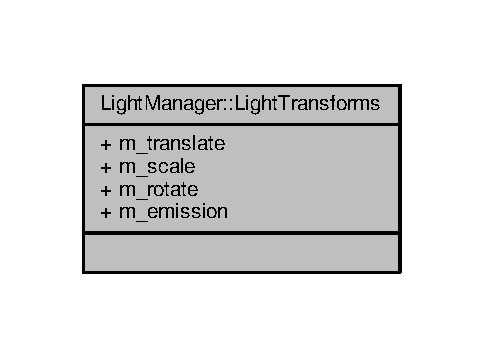
\includegraphics[width=232pt]{struct_light_manager_1_1_light_transforms__coll__graph}
\end{center}
\end{figure}
\subsection*{Public Attributes}
\begin{DoxyCompactItemize}
\item 
\hypertarget{struct_light_manager_1_1_light_transforms_aca910f0ba57d010927e00cd12636f63e}{glm\-::vec3 {\bfseries m\-\_\-translate}}\label{struct_light_manager_1_1_light_transforms_aca910f0ba57d010927e00cd12636f63e}

\item 
\hypertarget{struct_light_manager_1_1_light_transforms_a6a2cff465ce93d26f23913063f80b58c}{glm\-::vec3 {\bfseries m\-\_\-scale}}\label{struct_light_manager_1_1_light_transforms_a6a2cff465ce93d26f23913063f80b58c}

\item 
\hypertarget{struct_light_manager_1_1_light_transforms_a98c9bda7160c67256f26bcaff2b1a687}{glm\-::vec3 {\bfseries m\-\_\-rotate}}\label{struct_light_manager_1_1_light_transforms_a98c9bda7160c67256f26bcaff2b1a687}

\item 
\hypertarget{struct_light_manager_1_1_light_transforms_a221430a6b38142458c1ce66399d480bf}{glm\-::vec3 {\bfseries m\-\_\-emission}}\label{struct_light_manager_1_1_light_transforms_a221430a6b38142458c1ce66399d480bf}

\end{DoxyCompactItemize}


The documentation for this struct was generated from the following file\-:\begin{DoxyCompactItemize}
\item 
include/\-Lights/Light\-Manager.\-h\end{DoxyCompactItemize}

\hypertarget{class_ui_1_1_main_window}{\section{Ui\-:\-:Main\-Window Class Reference}
\label{class_ui_1_1_main_window}\index{Ui\-::\-Main\-Window@{Ui\-::\-Main\-Window}}
}


Inheritance diagram for Ui\-:\-:Main\-Window\-:
\nopagebreak
\begin{figure}[H]
\begin{center}
\leavevmode
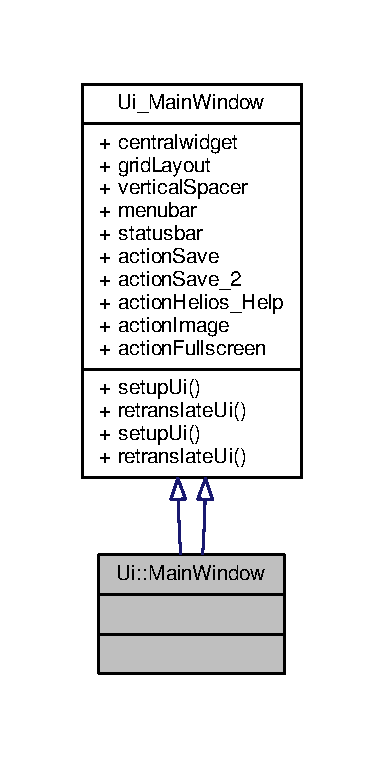
\includegraphics[width=184pt]{class_ui_1_1_main_window__inherit__graph}
\end{center}
\end{figure}


Collaboration diagram for Ui\-:\-:Main\-Window\-:
\nopagebreak
\begin{figure}[H]
\begin{center}
\leavevmode
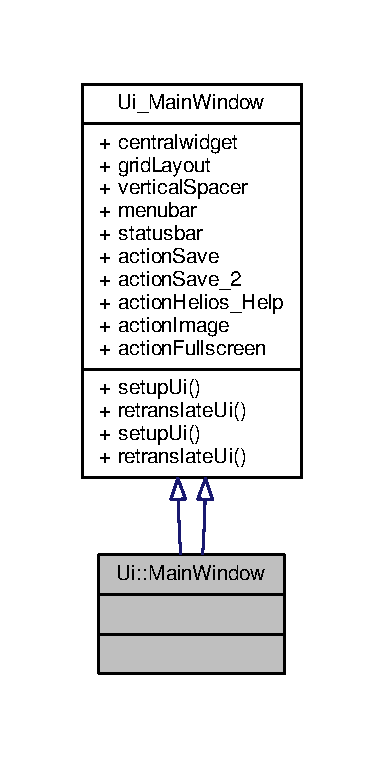
\includegraphics[width=184pt]{class_ui_1_1_main_window__coll__graph}
\end{center}
\end{figure}
\subsection*{Additional Inherited Members}


The documentation for this class was generated from the following file\-:\begin{DoxyCompactItemize}
\item 
include/ui\-\_\-mainwindow.\-h\end{DoxyCompactItemize}

\hypertarget{class_main_window}{\section{Main\-Window Class Reference}
\label{class_main_window}\index{Main\-Window@{Main\-Window}}
}


Inheritance diagram for Main\-Window\-:
\nopagebreak
\begin{figure}[H]
\begin{center}
\leavevmode
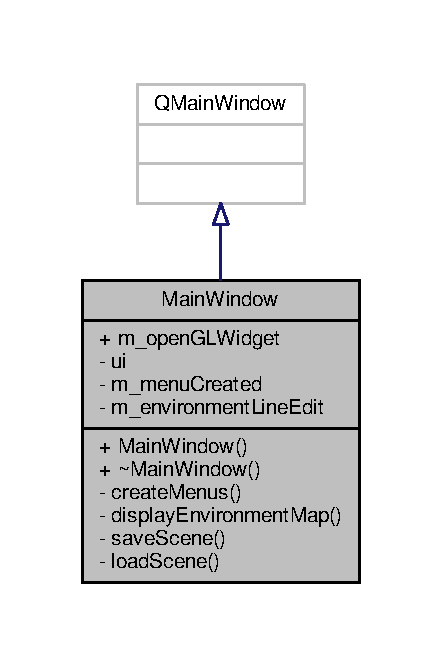
\includegraphics[width=212pt]{class_main_window__inherit__graph}
\end{center}
\end{figure}


Collaboration diagram for Main\-Window\-:
\nopagebreak
\begin{figure}[H]
\begin{center}
\leavevmode
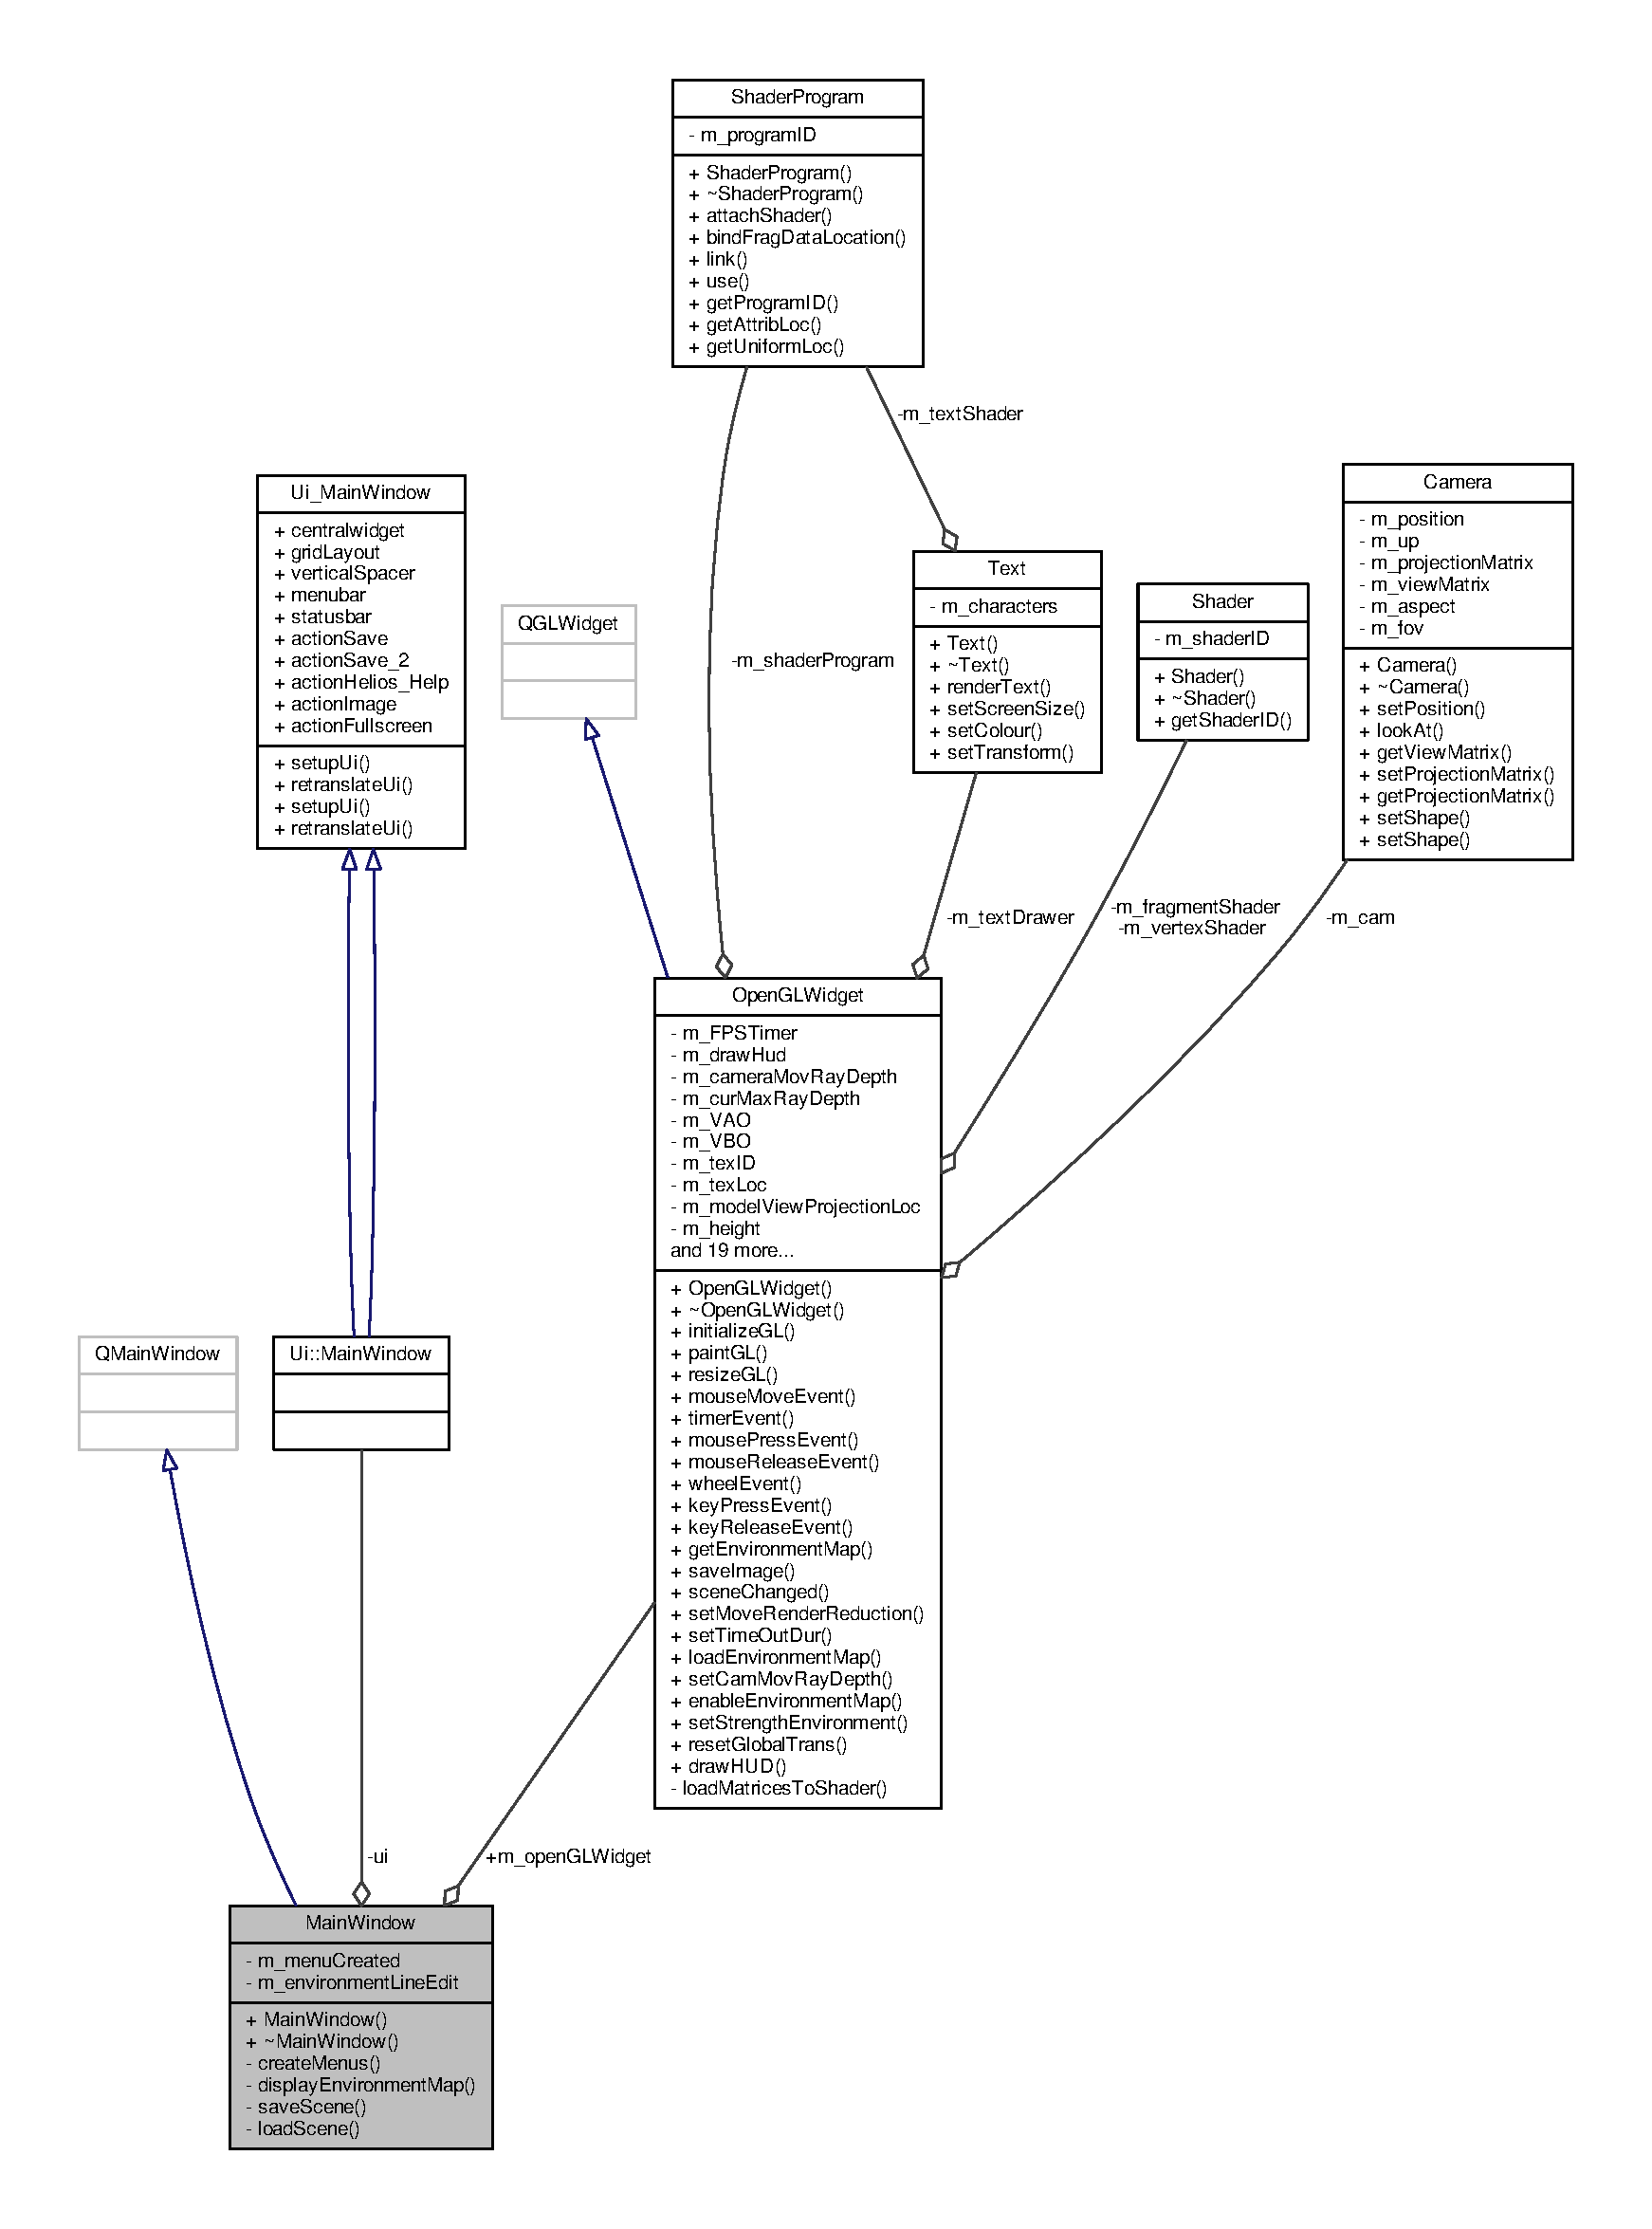
\includegraphics[width=350pt]{class_main_window__coll__graph}
\end{center}
\end{figure}
\subsection*{Signals}
\begin{DoxyCompactItemize}
\item 
\hypertarget{class_main_window_a236b3b5276d6982049ce4a8c32664611}{void \hyperlink{class_main_window_a236b3b5276d6982049ce4a8c32664611}{menus\-Created} ()}\label{class_main_window_a236b3b5276d6982049ce4a8c32664611}

\begin{DoxyCompactList}\small\item\em signals when our menues have been created \end{DoxyCompactList}\end{DoxyCompactItemize}
\subsection*{Public Member Functions}
\begin{DoxyCompactItemize}
\item 
\hypertarget{class_main_window_a8b244be8b7b7db1b08de2a2acb9409db}{\hyperlink{class_main_window_a8b244be8b7b7db1b08de2a2acb9409db}{Main\-Window} (Q\-Widget $\ast$parent=0)}\label{class_main_window_a8b244be8b7b7db1b08de2a2acb9409db}

\begin{DoxyCompactList}\small\item\em Constructor. \end{DoxyCompactList}\item 
\hypertarget{class_main_window_ae98d00a93bc118200eeef9f9bba1dba7}{\hyperlink{class_main_window_ae98d00a93bc118200eeef9f9bba1dba7}{$\sim$\-Main\-Window} ()}\label{class_main_window_ae98d00a93bc118200eeef9f9bba1dba7}

\begin{DoxyCompactList}\small\item\em Destructor. \end{DoxyCompactList}\end{DoxyCompactItemize}
\subsection*{Public Attributes}
\begin{DoxyCompactItemize}
\item 
\hypertarget{class_main_window_af310504f60344259d8a43e495e90e54d}{\hyperlink{class_open_g_l_widget}{Open\-G\-L\-Widget} $\ast$ \hyperlink{class_main_window_af310504f60344259d8a43e495e90e54d}{m\-\_\-open\-G\-L\-Widget}}\label{class_main_window_af310504f60344259d8a43e495e90e54d}

\begin{DoxyCompactList}\small\item\em Our Qt Open\-G\-L context. \end{DoxyCompactList}\end{DoxyCompactItemize}
\subsection*{Private Slots}
\begin{DoxyCompactItemize}
\item 
\hypertarget{class_main_window_aa4907b0251d305659e403c62921ef331}{void \hyperlink{class_main_window_aa4907b0251d305659e403c62921ef331}{create\-Menus} ()}\label{class_main_window_aa4907b0251d305659e403c62921ef331}

\begin{DoxyCompactList}\small\item\em Slot when called creates all our menus. \end{DoxyCompactList}\item 
\hypertarget{class_main_window_a392404296e4eb0b29ace84edbc6130b8}{void \hyperlink{class_main_window_a392404296e4eb0b29ace84edbc6130b8}{display\-Environment\-Map} ()}\label{class_main_window_a392404296e4eb0b29ace84edbc6130b8}

\begin{DoxyCompactList}\small\item\em display the enironment map name in the environment map line edit \end{DoxyCompactList}\item 
\hypertarget{class_main_window_a8c5c70395af911e771dbf61da52169ab}{void \hyperlink{class_main_window_a8c5c70395af911e771dbf61da52169ab}{save\-Scene} ()}\label{class_main_window_a8c5c70395af911e771dbf61da52169ab}

\begin{DoxyCompactList}\small\item\em saves our scene \end{DoxyCompactList}\item 
\hypertarget{class_main_window_abc2541016866f91904cb3aa64ca85a06}{void \hyperlink{class_main_window_abc2541016866f91904cb3aa64ca85a06}{load\-Scene} ()}\label{class_main_window_abc2541016866f91904cb3aa64ca85a06}

\begin{DoxyCompactList}\small\item\em load scene from a file \end{DoxyCompactList}\end{DoxyCompactItemize}
\subsection*{Private Attributes}
\begin{DoxyCompactItemize}
\item 
\hypertarget{class_main_window_a35466a70ed47252a0191168126a352a5}{\hyperlink{class_ui_1_1_main_window}{Ui\-::\-Main\-Window} $\ast$ \hyperlink{class_main_window_a35466a70ed47252a0191168126a352a5}{ui}}\label{class_main_window_a35466a70ed47252a0191168126a352a5}

\begin{DoxyCompactList}\small\item\em Main window U\-I. \end{DoxyCompactList}\item 
\hypertarget{class_main_window_a12d9561bbb394f11186597772d87bef5}{bool \hyperlink{class_main_window_a12d9561bbb394f11186597772d87bef5}{m\-\_\-menu\-Created}}\label{class_main_window_a12d9561bbb394f11186597772d87bef5}

\begin{DoxyCompactList}\small\item\em bool to indicate if our menues have been created \end{DoxyCompactList}\item 
\hypertarget{class_main_window_a048f5126b9a96e5611b520ab3c8bbb55}{Q\-Line\-Edit $\ast$ \hyperlink{class_main_window_a048f5126b9a96e5611b520ab3c8bbb55}{m\-\_\-environment\-Line\-Edit}}\label{class_main_window_a048f5126b9a96e5611b520ab3c8bbb55}

\begin{DoxyCompactList}\small\item\em A line edit to display environement map. \end{DoxyCompactList}\end{DoxyCompactItemize}


The documentation for this class was generated from the following files\-:\begin{DoxyCompactItemize}
\item 
include/\-Core/mainwindow.\-h\item 
moc/moc\-\_\-mainwindow.\-cpp\item 
src/\-Core/mainwindow.\-cpp\end{DoxyCompactItemize}

\hypertarget{class_material_library}{\section{Material\-Library Class Reference}
\label{class_material_library}\index{Material\-Library@{Material\-Library}}
}


A wigdet to store and allow the user to select between.  




{\ttfamily \#include $<$Material\-Library.\-h$>$}



Inheritance diagram for Material\-Library\-:
\nopagebreak
\begin{figure}[H]
\begin{center}
\leavevmode
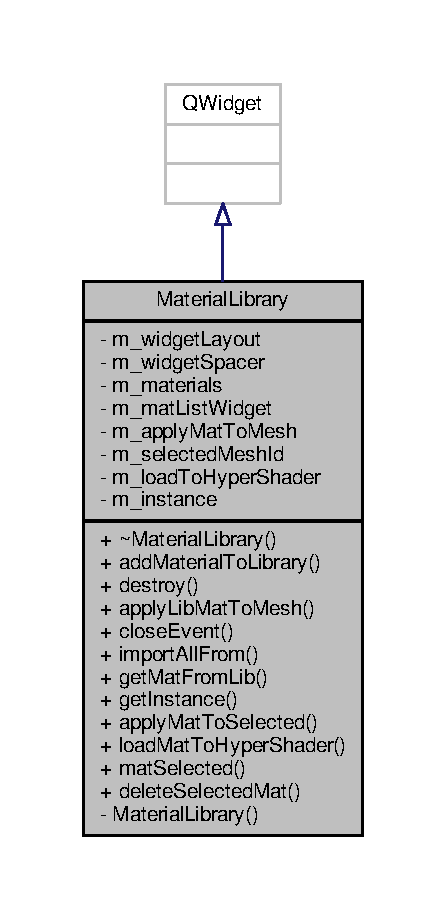
\includegraphics[width=214pt]{class_material_library__inherit__graph}
\end{center}
\end{figure}


Collaboration diagram for Material\-Library\-:
\nopagebreak
\begin{figure}[H]
\begin{center}
\leavevmode
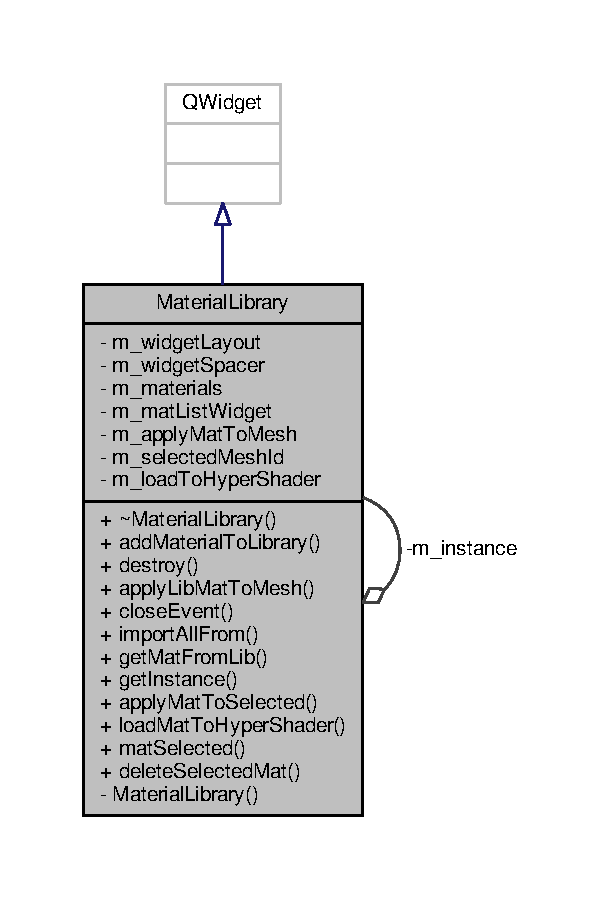
\includegraphics[width=289pt]{class_material_library__coll__graph}
\end{center}
\end{figure}
\subsection*{Public Slots}
\begin{DoxyCompactItemize}
\item 
\hypertarget{class_material_library_a25fbe1df01423d3c29f17b068c1fa93e}{void \hyperlink{class_material_library_a25fbe1df01423d3c29f17b068c1fa93e}{apply\-Mat\-To\-Selected} ()}\label{class_material_library_a25fbe1df01423d3c29f17b068c1fa93e}

\begin{DoxyCompactList}\small\item\em applys selected material to current selected in mesh widget \end{DoxyCompactList}\item 
\hypertarget{class_material_library_a0757b6c745d5796b30abcdb042ba1273}{void \hyperlink{class_material_library_a0757b6c745d5796b30abcdb042ba1273}{load\-Mat\-To\-Hyper\-Shader} ()}\label{class_material_library_a0757b6c745d5796b30abcdb042ba1273}

\begin{DoxyCompactList}\small\item\em functino to let the user select a material from our library to put in our node graph \end{DoxyCompactList}\item 
void \hyperlink{class_material_library_a2e77c2e90d100dec3a113c2ea1e94fb5}{mat\-Selected} (Q\-List\-Widget\-Item $\ast$\-\_\-item)
\begin{DoxyCompactList}\small\item\em slot to be called if something is selected in our material list \end{DoxyCompactList}\item 
\hypertarget{class_material_library_abc3c89c6bbf434a2ea9d21e70198f2ae}{void \hyperlink{class_material_library_abc3c89c6bbf434a2ea9d21e70198f2ae}{delete\-Selected\-Mat} ()}\label{class_material_library_abc3c89c6bbf434a2ea9d21e70198f2ae}

\begin{DoxyCompactList}\small\item\em slot to be called to delete selected materials in material library list \end{DoxyCompactList}\end{DoxyCompactItemize}
\subsection*{Public Member Functions}
\begin{DoxyCompactItemize}
\item 
\hypertarget{class_material_library_a8b0b82c532ada235ad3a74d623345600}{\hyperlink{class_material_library_a8b0b82c532ada235ad3a74d623345600}{$\sim$\-Material\-Library} ()}\label{class_material_library_a8b0b82c532ada235ad3a74d623345600}

\begin{DoxyCompactList}\small\item\em default destructor. Deals with our garbage collection \end{DoxyCompactList}\item 
bool \hyperlink{class_material_library_a6ed4adc6fb885d3a7cd69437117092c6}{add\-Material\-To\-Library} (std\-::string \-\_\-name, optix\-::\-Material \-\_\-material)
\begin{DoxyCompactList}\small\item\em add a material to our library \end{DoxyCompactList}\item 
\hypertarget{class_material_library_ad5e0c33418b4554c7167d8cff539f951}{void \hyperlink{class_material_library_ad5e0c33418b4554c7167d8cff539f951}{destroy} ()}\label{class_material_library_ad5e0c33418b4554c7167d8cff539f951}

\begin{DoxyCompactList}\small\item\em removes our singleton class from existance \end{DoxyCompactList}\item 
void \hyperlink{class_material_library_a505e48b500d1d04f6445c423a2fe66ac}{apply\-Lib\-Mat\-To\-Mesh} (std\-::string \-\_\-mesh\-Id)
\begin{DoxyCompactList}\small\item\em function let the user select a material from our library and apply it to a mesh \end{DoxyCompactList}\item 
\hypertarget{class_material_library_a7fa5922dfa78d16fafa8dc79ddaf427e}{void \hyperlink{class_material_library_a7fa5922dfa78d16fafa8dc79ddaf427e}{close\-Event} (Q\-Close\-Event $\ast$event)}\label{class_material_library_a7fa5922dfa78d16fafa8dc79ddaf427e}

\begin{DoxyCompactList}\small\item\em overide our close event to reset our variables \end{DoxyCompactList}\item 
\hypertarget{class_material_library_a93a390e382f15c20a3ba3d760cdb4bc5}{void \hyperlink{class_material_library_a93a390e382f15c20a3ba3d760cdb4bc5}{import\-All\-From} (Q\-String \-\_\-path)}\label{class_material_library_a93a390e382f15c20a3ba3d760cdb4bc5}

\begin{DoxyCompactList}\small\item\em imports all materials from a directory \end{DoxyCompactList}\item 
bool \hyperlink{class_material_library_a0d8235104709564a600a6ece7ea048ae}{get\-Mat\-From\-Lib} (std\-::string \-\_\-mat, optix\-::\-Material \&o\-\_\-mat)
\begin{DoxyCompactList}\small\item\em returns a queried material from library if it exits \end{DoxyCompactList}\end{DoxyCompactItemize}
\subsection*{Static Public Member Functions}
\begin{DoxyCompactItemize}
\item 
\hypertarget{class_material_library_a9dddb26d8ba882414f96bf5e4e6c3cf6}{static \hyperlink{class_material_library}{Material\-Library} $\ast$ \hyperlink{class_material_library_a9dddb26d8ba882414f96bf5e4e6c3cf6}{get\-Instance} (Q\-Widget $\ast$parent=0)}\label{class_material_library_a9dddb26d8ba882414f96bf5e4e6c3cf6}

\begin{DoxyCompactList}\small\item\em get an instance of our material library \end{DoxyCompactList}\end{DoxyCompactItemize}
\subsection*{Private Member Functions}
\begin{DoxyCompactItemize}
\item 
\hypertarget{class_material_library_ac0fdd21aa44b30e4ef14f252f26c3f1e}{\hyperlink{class_material_library_ac0fdd21aa44b30e4ef14f252f26c3f1e}{Material\-Library} (Q\-Widget $\ast$parent=0)}\label{class_material_library_ac0fdd21aa44b30e4ef14f252f26c3f1e}

\begin{DoxyCompactList}\small\item\em defalut constructor \end{DoxyCompactList}\end{DoxyCompactItemize}
\subsection*{Private Attributes}
\begin{DoxyCompactItemize}
\item 
\hypertarget{class_material_library_acc7cbee72728cb17b9dc46c6eb181235}{Q\-Grid\-Layout $\ast$ \hyperlink{class_material_library_acc7cbee72728cb17b9dc46c6eb181235}{m\-\_\-widget\-Layout}}\label{class_material_library_acc7cbee72728cb17b9dc46c6eb181235}

\begin{DoxyCompactList}\small\item\em the layout of our wigdet \end{DoxyCompactList}\item 
\hypertarget{class_material_library_a68a1b4d7a9cae065772845db125fee27}{Q\-Spacer\-Item $\ast$ \hyperlink{class_material_library_a68a1b4d7a9cae065772845db125fee27}{m\-\_\-widget\-Spacer}}\label{class_material_library_a68a1b4d7a9cae065772845db125fee27}

\begin{DoxyCompactList}\small\item\em spacer for our widget \end{DoxyCompactList}\item 
\hypertarget{class_material_library_af25abb43cda644364bc7faefbd957f9d}{std\-::map$<$ std\-::string, \\*
optix\-::\-Material $>$ \hyperlink{class_material_library_af25abb43cda644364bc7faefbd957f9d}{m\-\_\-materials}}\label{class_material_library_af25abb43cda644364bc7faefbd957f9d}

\begin{DoxyCompactList}\small\item\em map of our materials \end{DoxyCompactList}\item 
\hypertarget{class_material_library_a6a4c3021bf23b7048bbb5ef82c66d9dd}{Q\-List\-Widget $\ast$ \hyperlink{class_material_library_a6a4c3021bf23b7048bbb5ef82c66d9dd}{m\-\_\-mat\-List\-Widget}}\label{class_material_library_a6a4c3021bf23b7048bbb5ef82c66d9dd}

\begin{DoxyCompactList}\small\item\em list widget to display the materials in our library \end{DoxyCompactList}\item 
\hypertarget{class_material_library_ab1dded7ae6d88f5407e29af6f68caf4a}{bool \hyperlink{class_material_library_ab1dded7ae6d88f5407e29af6f68caf4a}{m\-\_\-apply\-Mat\-To\-Mesh}}\label{class_material_library_ab1dded7ae6d88f5407e29af6f68caf4a}

\begin{DoxyCompactList}\small\item\em a bool to indicate if we are applying the next selected material to a mesh \end{DoxyCompactList}\item 
\hypertarget{class_material_library_a6ee155650b6bbf4b3b959fa2b931ad7d}{std\-::string \hyperlink{class_material_library_a6ee155650b6bbf4b3b959fa2b931ad7d}{m\-\_\-selected\-Mesh\-Id}}\label{class_material_library_a6ee155650b6bbf4b3b959fa2b931ad7d}

\begin{DoxyCompactList}\small\item\em mesh to apply material to \end{DoxyCompactList}\item 
\hypertarget{class_material_library_aa095023b0334021154906729f0cba732}{bool \hyperlink{class_material_library_aa095023b0334021154906729f0cba732}{m\-\_\-load\-To\-Hyper\-Shader}}\label{class_material_library_aa095023b0334021154906729f0cba732}

\begin{DoxyCompactList}\small\item\em a bool to indicate if we are importing our material to our hypershader \end{DoxyCompactList}\end{DoxyCompactItemize}
\subsection*{Static Private Attributes}
\begin{DoxyCompactItemize}
\item 
\hypertarget{class_material_library_aef4ba3f093412e83f5da295865f8b508}{static \hyperlink{class_material_library}{Material\-Library} $\ast$ \hyperlink{class_material_library_aef4ba3f093412e83f5da295865f8b508}{m\-\_\-instance}}\label{class_material_library_aef4ba3f093412e83f5da295865f8b508}

\begin{DoxyCompactList}\small\item\em pointer to the instance of our singleton class \end{DoxyCompactList}\end{DoxyCompactItemize}


\subsection{Detailed Description}
A wigdet to store and allow the user to select between. 

\begin{DoxyAuthor}{Author}
Declan Russell 
\end{DoxyAuthor}
\begin{DoxyDate}{Date}
05/03/15 optix materials availible in out program. This is a singleton class as we want all instances of our library to be the same. 
\end{DoxyDate}


\subsection{Member Function Documentation}
\hypertarget{class_material_library_a6ed4adc6fb885d3a7cd69437117092c6}{\index{Material\-Library@{Material\-Library}!add\-Material\-To\-Library@{add\-Material\-To\-Library}}
\index{add\-Material\-To\-Library@{add\-Material\-To\-Library}!MaterialLibrary@{Material\-Library}}
\subsubsection[{add\-Material\-To\-Library}]{\setlength{\rightskip}{0pt plus 5cm}bool Material\-Library\-::add\-Material\-To\-Library (
\begin{DoxyParamCaption}
\item[{std\-::string}]{\-\_\-name, }
\item[{optix\-::\-Material}]{\-\_\-material}
\end{DoxyParamCaption}
)}}\label{class_material_library_a6ed4adc6fb885d3a7cd69437117092c6}


add a material to our library 


\begin{DoxyParams}{Parameters}
{\em \-\_\-name} & -\/ the name of the material to add \\
\hline
{\em \-\_\-material} & -\/ the optix material to add to the library \\
\hline
\end{DoxyParams}
\begin{DoxyReturn}{Returns}
bool indicating if the material has been successfully added to the library 
\end{DoxyReturn}


Here is the caller graph for this function\-:
\nopagebreak
\begin{figure}[H]
\begin{center}
\leavevmode
\includegraphics[width=350pt]{class_material_library_a6ed4adc6fb885d3a7cd69437117092c6_icgraph}
\end{center}
\end{figure}


\hypertarget{class_material_library_a505e48b500d1d04f6445c423a2fe66ac}{\index{Material\-Library@{Material\-Library}!apply\-Lib\-Mat\-To\-Mesh@{apply\-Lib\-Mat\-To\-Mesh}}
\index{apply\-Lib\-Mat\-To\-Mesh@{apply\-Lib\-Mat\-To\-Mesh}!MaterialLibrary@{Material\-Library}}
\subsubsection[{apply\-Lib\-Mat\-To\-Mesh}]{\setlength{\rightskip}{0pt plus 5cm}void Material\-Library\-::apply\-Lib\-Mat\-To\-Mesh (
\begin{DoxyParamCaption}
\item[{std\-::string}]{\-\_\-mesh\-Id}
\end{DoxyParamCaption}
)}}\label{class_material_library_a505e48b500d1d04f6445c423a2fe66ac}


function let the user select a material from our library and apply it to a mesh 


\begin{DoxyParams}{Parameters}
{\em \-\_\-mesh\-Id} & -\/ id of mesh to apply it to \\
\hline
\end{DoxyParams}


Here is the caller graph for this function\-:
\nopagebreak
\begin{figure}[H]
\begin{center}
\leavevmode
\includegraphics[width=350pt]{class_material_library_a505e48b500d1d04f6445c423a2fe66ac_icgraph}
\end{center}
\end{figure}


\hypertarget{class_material_library_a0d8235104709564a600a6ece7ea048ae}{\index{Material\-Library@{Material\-Library}!get\-Mat\-From\-Lib@{get\-Mat\-From\-Lib}}
\index{get\-Mat\-From\-Lib@{get\-Mat\-From\-Lib}!MaterialLibrary@{Material\-Library}}
\subsubsection[{get\-Mat\-From\-Lib}]{\setlength{\rightskip}{0pt plus 5cm}bool Material\-Library\-::get\-Mat\-From\-Lib (
\begin{DoxyParamCaption}
\item[{std\-::string}]{\-\_\-mat, }
\item[{optix\-::\-Material \&}]{o\-\_\-mat}
\end{DoxyParamCaption}
)}}\label{class_material_library_a0d8235104709564a600a6ece7ea048ae}


returns a queried material from library if it exits 


\begin{DoxyParams}{Parameters}
{\em \-\_\-mat} & -\/ name of material to be queried \\
\hline
{\em o\-\_\-mat} & -\/ handle of found material \\
\hline
\end{DoxyParams}
\begin{DoxyReturn}{Returns}
true is material is found 
\end{DoxyReturn}


Here is the caller graph for this function\-:
\nopagebreak
\begin{figure}[H]
\begin{center}
\leavevmode
\includegraphics[width=350pt]{class_material_library_a0d8235104709564a600a6ece7ea048ae_icgraph}
\end{center}
\end{figure}


\hypertarget{class_material_library_a2e77c2e90d100dec3a113c2ea1e94fb5}{\index{Material\-Library@{Material\-Library}!mat\-Selected@{mat\-Selected}}
\index{mat\-Selected@{mat\-Selected}!MaterialLibrary@{Material\-Library}}
\subsubsection[{mat\-Selected}]{\setlength{\rightskip}{0pt plus 5cm}void Material\-Library\-::mat\-Selected (
\begin{DoxyParamCaption}
\item[{Q\-List\-Widget\-Item $\ast$}]{\-\_\-item}
\end{DoxyParamCaption}
)\hspace{0.3cm}{\ttfamily [slot]}}}\label{class_material_library_a2e77c2e90d100dec3a113c2ea1e94fb5}


slot to be called if something is selected in our material list 


\begin{DoxyParams}{Parameters}
{\em \-\_\-item} & -\/ item selected in list \\
\hline
\end{DoxyParams}


Here is the call graph for this function\-:
\nopagebreak
\begin{figure}[H]
\begin{center}
\leavevmode
\includegraphics[width=350pt]{class_material_library_a2e77c2e90d100dec3a113c2ea1e94fb5_cgraph}
\end{center}
\end{figure}




Here is the caller graph for this function\-:
\nopagebreak
\begin{figure}[H]
\begin{center}
\leavevmode
\includegraphics[width=350pt]{class_material_library_a2e77c2e90d100dec3a113c2ea1e94fb5_icgraph}
\end{center}
\end{figure}




The documentation for this class was generated from the following files\-:\begin{DoxyCompactItemize}
\item 
include/\-Core/Material\-Library.\-h\item 
src/\-Core/Material\-Library.\-cpp\end{DoxyCompactItemize}

\hypertarget{class_mesh_widget}{\section{Mesh\-Widget Class Reference}
\label{class_mesh_widget}\index{Mesh\-Widget@{Mesh\-Widget}}
}


This class is an extention of Q\-Dock\-Widget that includes our camera controls.  




{\ttfamily \#include $<$Camera\-Widget.\-h$>$}



Inheritance diagram for Mesh\-Widget\-:
\nopagebreak
\begin{figure}[H]
\begin{center}
\leavevmode
\includegraphics[height=550pt]{class_mesh_widget__inherit__graph}
\end{center}
\end{figure}


Collaboration diagram for Mesh\-Widget\-:
\nopagebreak
\begin{figure}[H]
\begin{center}
\leavevmode
\includegraphics[height=550pt]{class_mesh_widget__coll__graph}
\end{center}
\end{figure}
\subsection*{Classes}
\begin{DoxyCompactItemize}
\item 
struct \hyperlink{struct_mesh_widget_1_1model_prop}{model\-Prop}
\begin{DoxyCompactList}\small\item\em structure for our model properties \end{DoxyCompactList}\end{DoxyCompactItemize}
\subsection*{Public Slots}
\begin{DoxyCompactItemize}
\item 
\hypertarget{class_mesh_widget_a6f5f317f243ea5c06b235af97edf6f49}{void \hyperlink{class_mesh_widget_a6f5f317f243ea5c06b235af97edf6f49}{clear\-Scene} ()}\label{class_mesh_widget_a6f5f317f243ea5c06b235af97edf6f49}

\begin{DoxyCompactList}\small\item\em clears all models in our scene \end{DoxyCompactList}\item 
\hypertarget{class_mesh_widget_ad31fbdeac98ac757b6fc8f1a6dccb197}{void \hyperlink{class_mesh_widget_ad31fbdeac98ac757b6fc8f1a6dccb197}{signal\-Transform\-Change} (double \-\_\-val=0)}\label{class_mesh_widget_ad31fbdeac98ac757b6fc8f1a6dccb197}

\begin{DoxyCompactList}\small\item\em our slot to notify if any tranform spinbox have been changed \end{DoxyCompactList}\item 
\hypertarget{class_mesh_widget_af819cb26a8a0ed4b6aa86fdf6a7c8bc7}{void \hyperlink{class_mesh_widget_af819cb26a8a0ed4b6aa86fdf6a7c8bc7}{apply\-O\-S\-L\-Material} (optix\-::\-Material \-\_\-mat, std\-::string \-\_\-mat\-Name)}\label{class_mesh_widget_af819cb26a8a0ed4b6aa86fdf6a7c8bc7}

\begin{DoxyCompactList}\small\item\em applys material to currently selected model \end{DoxyCompactList}\item 
\hypertarget{class_mesh_widget_aac3bcbbfb389bf17505d4eb894ae5693}{void \hyperlink{class_mesh_widget_aac3bcbbfb389bf17505d4eb894ae5693}{apply\-Mat\-From\-Lib} ()}\label{class_mesh_widget_aac3bcbbfb389bf17505d4eb894ae5693}

\begin{DoxyCompactList}\small\item\em applies material from library to mesh \end{DoxyCompactList}\item 
\hypertarget{class_mesh_widget_a771417b5002a0e5e9cfb32553b7f7544}{void \hyperlink{class_mesh_widget_a771417b5002a0e5e9cfb32553b7f7544}{import\-Model} ()}\label{class_mesh_widget_a771417b5002a0e5e9cfb32553b7f7544}

\begin{DoxyCompactList}\small\item\em slot to import a model \end{DoxyCompactList}\item 
void \hyperlink{class_mesh_widget_afc878f28393e7e918e5d88f6a747d22a}{model\-Selected} (Q\-List\-Widget\-Item $\ast$\-\_\-item)
\begin{DoxyCompactList}\small\item\em slot for if a item is selected from our list \end{DoxyCompactList}\item 
\hypertarget{class_mesh_widget_a39e961759059b54abc380b149f0186f8}{void \hyperlink{class_mesh_widget_a39e961759059b54abc380b149f0186f8}{create\-Instance} ()}\label{class_mesh_widget_a39e961759059b54abc380b149f0186f8}

\begin{DoxyCompactList}\small\item\em slot to create instance of geometry selected \end{DoxyCompactList}\item 
\hypertarget{class_mesh_widget_a4e934e8f2eb83349fe0b865f4c242e3d}{void \hyperlink{class_mesh_widget_a4e934e8f2eb83349fe0b865f4c242e3d}{remove\-Selected} ()}\label{class_mesh_widget_a4e934e8f2eb83349fe0b865f4c242e3d}

\begin{DoxyCompactList}\small\item\em slot to remove selected geometry \end{DoxyCompactList}\end{DoxyCompactItemize}
\subsection*{Signals}
\begin{DoxyCompactItemize}
\item 
\hypertarget{class_mesh_widget_adfc6c88e47a65d0e41b7b1f4b4db216d}{void \hyperlink{class_mesh_widget_adfc6c88e47a65d0e41b7b1f4b4db216d}{update\-Scene} ()}\label{class_mesh_widget_adfc6c88e47a65d0e41b7b1f4b4db216d}

\begin{DoxyCompactList}\small\item\em a signal called when something has changed to promt the update of our scene \end{DoxyCompactList}\end{DoxyCompactItemize}
\subsection*{Public Member Functions}
\begin{DoxyCompactItemize}
\item 
void \hyperlink{class_mesh_widget_a67ebdf43ebd7ada4ef14d0c72f6a2f35}{save} (Q\-Data\-Stream \&ds)
\begin{DoxyCompactList}\small\item\em saves the objects in our scene to file \end{DoxyCompactList}\item 
void \hyperlink{class_mesh_widget_a47bdbf5350b44dd43a08e27b16c407d7}{load} (Q\-Data\-Stream \&ds)
\begin{DoxyCompactList}\small\item\em loads scene from file \end{DoxyCompactList}\item 
\hypertarget{class_mesh_widget_a456ac85d510b5700f60877a5466d0311}{int \hyperlink{class_mesh_widget_a456ac85d510b5700f60877a5466d0311}{get\-Num\-Models} ()}\label{class_mesh_widget_a456ac85d510b5700f60877a5466d0311}

\begin{DoxyCompactList}\small\item\em returns the number of models in our scene \end{DoxyCompactList}\end{DoxyCompactItemize}
\subsection*{Static Public Member Functions}
\begin{DoxyCompactItemize}
\item 
\hypertarget{class_mesh_widget_ab69e785150bd1802124a3fea62940866}{static \hyperlink{class_mesh_widget}{Mesh\-Widget} $\ast$ \hyperlink{class_mesh_widget_ab69e785150bd1802124a3fea62940866}{get\-Instance} (Q\-Widget $\ast$parent=0)}\label{class_mesh_widget_ab69e785150bd1802124a3fea62940866}

\begin{DoxyCompactList}\small\item\em returns the instance of our mesh widget \end{DoxyCompactList}\item 
\hypertarget{class_mesh_widget_a39971ebf92a18d4d2a975fcefab82c91}{static void \hyperlink{class_mesh_widget_a39971ebf92a18d4d2a975fcefab82c91}{destroy} ()}\label{class_mesh_widget_a39971ebf92a18d4d2a975fcefab82c91}

\begin{DoxyCompactList}\small\item\em destroys our singleton class \end{DoxyCompactList}\end{DoxyCompactItemize}
\subsection*{Private Member Functions}
\begin{DoxyCompactItemize}
\item 
\hypertarget{class_mesh_widget_ab914a1597ebaa0b2679f9ae32226ab3f}{\hyperlink{class_mesh_widget_ab914a1597ebaa0b2679f9ae32226ab3f}{$\sim$\-Mesh\-Widget} ()}\label{class_mesh_widget_ab914a1597ebaa0b2679f9ae32226ab3f}

\begin{DoxyCompactList}\small\item\em our destructor \end{DoxyCompactList}\item 
\hypertarget{class_mesh_widget_a2a83b4ce21ff9a33d5b7315faefb8fed}{\hyperlink{class_mesh_widget_a2a83b4ce21ff9a33d5b7315faefb8fed}{Mesh\-Widget} (Q\-Widget $\ast$parent=0)}\label{class_mesh_widget_a2a83b4ce21ff9a33d5b7315faefb8fed}

\begin{DoxyCompactList}\small\item\em our default constructor \end{DoxyCompactList}\end{DoxyCompactItemize}
\subsection*{Private Attributes}
\begin{DoxyCompactItemize}
\item 
\hypertarget{class_mesh_widget_aa919bf9e1a8f87a2f88beb5bebcc8365}{bool \hyperlink{class_mesh_widget_aa919bf9e1a8f87a2f88beb5bebcc8365}{m\-\_\-update}}\label{class_mesh_widget_aa919bf9e1a8f87a2f88beb5bebcc8365}

\begin{DoxyCompactList}\small\item\em bool to define if we want to be able to update models translation \end{DoxyCompactList}\item 
\hypertarget{class_mesh_widget_a5db4abbd4581a08f7e0cab81a36672a9}{std\-::map$<$ Q\-String, \hyperlink{struct_mesh_widget_1_1model_prop}{model\-Prop} $\ast$ $>$ \hyperlink{class_mesh_widget_a5db4abbd4581a08f7e0cab81a36672a9}{m\-\_\-model\-Properties}}\label{class_mesh_widget_a5db4abbd4581a08f7e0cab81a36672a9}

\begin{DoxyCompactList}\small\item\em map of our model properties \end{DoxyCompactList}\item 
\hypertarget{class_mesh_widget_aa9bc3fcd1cabd6c762c1592bba3ecb3d}{\hyperlink{struct_mesh_widget_1_1model_prop}{model\-Prop} $\ast$ \hyperlink{class_mesh_widget_aa9bc3fcd1cabd6c762c1592bba3ecb3d}{m\-\_\-cur\-Model\-Prop}}\label{class_mesh_widget_aa9bc3fcd1cabd6c762c1592bba3ecb3d}

\begin{DoxyCompactList}\small\item\em our current model properties \end{DoxyCompactList}\item 
\hypertarget{class_mesh_widget_aeb16152b584efae49428f395ae71d255}{Q\-List\-Widget $\ast$ \hyperlink{class_mesh_widget_aeb16152b584efae49428f395ae71d255}{m\-\_\-model\-List}}\label{class_mesh_widget_aeb16152b584efae49428f395ae71d255}

\begin{DoxyCompactList}\small\item\em List Widget to give U\-I to our models. \end{DoxyCompactList}\item 
\hypertarget{class_mesh_widget_a2a90703bcfd2bfba0f177763b9492bde}{Q\-Spacer\-Item $\ast$ \hyperlink{class_mesh_widget_a2a90703bcfd2bfba0f177763b9492bde}{m\-\_\-mesh\-Spacer}}\label{class_mesh_widget_a2a90703bcfd2bfba0f177763b9492bde}

\begin{DoxyCompactList}\small\item\em our spacer for the widget \end{DoxyCompactList}\item 
\hypertarget{class_mesh_widget_a04fd332bcf722b71c2da1e05b1f1dde6}{Q\-Double\-Spin\-Box $\ast$ \hyperlink{class_mesh_widget_a04fd332bcf722b71c2da1e05b1f1dde6}{m\-\_\-mesh\-Rotate\-X\-D\-Spin\-Box}}\label{class_mesh_widget_a04fd332bcf722b71c2da1e05b1f1dde6}

\begin{DoxyCompactList}\small\item\em our spinbox for x rotation \end{DoxyCompactList}\item 
\hypertarget{class_mesh_widget_a69d18769fc96a008437a072e29a2d6d2}{Q\-Double\-Spin\-Box $\ast$ \hyperlink{class_mesh_widget_a69d18769fc96a008437a072e29a2d6d2}{m\-\_\-mesh\-Rotate\-Y\-D\-Spin\-Box}}\label{class_mesh_widget_a69d18769fc96a008437a072e29a2d6d2}

\begin{DoxyCompactList}\small\item\em our spinbox for y rotation \end{DoxyCompactList}\item 
\hypertarget{class_mesh_widget_a5e41ed433f956c32749a2667337cb2b0}{Q\-Double\-Spin\-Box $\ast$ \hyperlink{class_mesh_widget_a5e41ed433f956c32749a2667337cb2b0}{m\-\_\-mesh\-Rotate\-Z\-D\-Spin\-Box}}\label{class_mesh_widget_a5e41ed433f956c32749a2667337cb2b0}

\begin{DoxyCompactList}\small\item\em our spinbox for z rotation \end{DoxyCompactList}\item 
\hypertarget{class_mesh_widget_aecdcbe099985d8e399a54cdfbe4698ff}{Q\-Double\-Spin\-Box $\ast$ \hyperlink{class_mesh_widget_aecdcbe099985d8e399a54cdfbe4698ff}{m\-\_\-mesh\-Translate\-X\-D\-Spin\-Box}}\label{class_mesh_widget_aecdcbe099985d8e399a54cdfbe4698ff}

\begin{DoxyCompactList}\small\item\em our spinbox for x translation \end{DoxyCompactList}\item 
\hypertarget{class_mesh_widget_a931d6dc6dbe58dda28e096455303582f}{Q\-Double\-Spin\-Box $\ast$ \hyperlink{class_mesh_widget_a931d6dc6dbe58dda28e096455303582f}{m\-\_\-mesh\-Translate\-Y\-D\-Spin\-Box}}\label{class_mesh_widget_a931d6dc6dbe58dda28e096455303582f}

\begin{DoxyCompactList}\small\item\em our spinbox for y translation \end{DoxyCompactList}\item 
\hypertarget{class_mesh_widget_ad421ee8459363aaa4641a629e14c8d3e}{Q\-Double\-Spin\-Box $\ast$ \hyperlink{class_mesh_widget_ad421ee8459363aaa4641a629e14c8d3e}{m\-\_\-mesh\-Translate\-Z\-D\-Spin\-Box}}\label{class_mesh_widget_ad421ee8459363aaa4641a629e14c8d3e}

\begin{DoxyCompactList}\small\item\em our spinbox for z translation \end{DoxyCompactList}\item 
\hypertarget{class_mesh_widget_ad0727eeb3046c2a4e219dc0702b02f4a}{Q\-Double\-Spin\-Box $\ast$ \hyperlink{class_mesh_widget_ad0727eeb3046c2a4e219dc0702b02f4a}{m\-\_\-mesh\-Scale\-X\-D\-Spin\-Box}}\label{class_mesh_widget_ad0727eeb3046c2a4e219dc0702b02f4a}

\begin{DoxyCompactList}\small\item\em our spinbox for x scale \end{DoxyCompactList}\item 
\hypertarget{class_mesh_widget_abbbc813dffc7918cdc1575ecfc8d9059}{Q\-Double\-Spin\-Box $\ast$ \hyperlink{class_mesh_widget_abbbc813dffc7918cdc1575ecfc8d9059}{m\-\_\-mesh\-Scale\-Y\-D\-Spin\-Box}}\label{class_mesh_widget_abbbc813dffc7918cdc1575ecfc8d9059}

\begin{DoxyCompactList}\small\item\em our spinbox for Y scale \end{DoxyCompactList}\item 
\hypertarget{class_mesh_widget_a39ffc5b350c23735bb883366975289e0}{Q\-Double\-Spin\-Box $\ast$ \hyperlink{class_mesh_widget_a39ffc5b350c23735bb883366975289e0}{m\-\_\-mesh\-Scale\-Z\-D\-Spin\-Box}}\label{class_mesh_widget_a39ffc5b350c23735bb883366975289e0}

\begin{DoxyCompactList}\small\item\em our spinbox for z scale \end{DoxyCompactList}\item 
\hypertarget{class_mesh_widget_a601eabcfd24a5918de58f19a6911bfcd}{Q\-String \hyperlink{class_mesh_widget_a601eabcfd24a5918de58f19a6911bfcd}{m\-\_\-cur\-Mesh\-Name}}\label{class_mesh_widget_a601eabcfd24a5918de58f19a6911bfcd}

\begin{DoxyCompactList}\small\item\em current mesh name \end{DoxyCompactList}\end{DoxyCompactItemize}
\subsection*{Static Private Attributes}
\begin{DoxyCompactItemize}
\item 
\hypertarget{class_mesh_widget_aafa751fb28e452ccaa5cbe83fa3b287b}{static \hyperlink{class_mesh_widget}{Mesh\-Widget} $\ast$ \hyperlink{class_mesh_widget_aafa751fb28e452ccaa5cbe83fa3b287b}{m\-\_\-instance}}\label{class_mesh_widget_aafa751fb28e452ccaa5cbe83fa3b287b}

\begin{DoxyCompactList}\small\item\em pointer to the instance of our singleton class \end{DoxyCompactList}\end{DoxyCompactItemize}


\subsection{Detailed Description}
This class is an extention of Q\-Dock\-Widget that includes our camera controls. 

A simple widget for rendering out images from our path tracer.

This class is an extention of Q\-Widget that adds all our mesh properties controls as default.

\begin{DoxyDate}{Date}
02/05/15 
\end{DoxyDate}
\begin{DoxyAuthor}{Author}
Toby Gilbert
\end{DoxyAuthor}
\begin{DoxyDate}{Date}
29/01/14 
\end{DoxyDate}
\begin{DoxyAuthor}{Author}
Declan Russell
\end{DoxyAuthor}
\begin{DoxyDate}{Date}
18/05/15 
\end{DoxyDate}
\begin{DoxyAuthor}{Author}
Declan Russell 
\end{DoxyAuthor}


\subsection{Member Function Documentation}
\hypertarget{class_mesh_widget_a47bdbf5350b44dd43a08e27b16c407d7}{\index{Mesh\-Widget@{Mesh\-Widget}!load@{load}}
\index{load@{load}!MeshWidget@{Mesh\-Widget}}
\subsubsection[{load}]{\setlength{\rightskip}{0pt plus 5cm}void Mesh\-Widget\-::load (
\begin{DoxyParamCaption}
\item[{Q\-Data\-Stream \&}]{ds}
\end{DoxyParamCaption}
)}}\label{class_mesh_widget_a47bdbf5350b44dd43a08e27b16c407d7}


loads scene from file 


\begin{DoxyParams}{Parameters}
{\em ds} & -\/ Q\-Data\-Stream of file \\
\hline
\end{DoxyParams}


Here is the call graph for this function\-:
\nopagebreak
\begin{figure}[H]
\begin{center}
\leavevmode
\includegraphics[width=350pt]{class_mesh_widget_a47bdbf5350b44dd43a08e27b16c407d7_cgraph}
\end{center}
\end{figure}




Here is the caller graph for this function\-:
\nopagebreak
\begin{figure}[H]
\begin{center}
\leavevmode
\includegraphics[width=350pt]{class_mesh_widget_a47bdbf5350b44dd43a08e27b16c407d7_icgraph}
\end{center}
\end{figure}


\hypertarget{class_mesh_widget_afc878f28393e7e918e5d88f6a747d22a}{\index{Mesh\-Widget@{Mesh\-Widget}!model\-Selected@{model\-Selected}}
\index{model\-Selected@{model\-Selected}!MeshWidget@{Mesh\-Widget}}
\subsubsection[{model\-Selected}]{\setlength{\rightskip}{0pt plus 5cm}void Mesh\-Widget\-::model\-Selected (
\begin{DoxyParamCaption}
\item[{Q\-List\-Widget\-Item $\ast$}]{\-\_\-item}
\end{DoxyParamCaption}
)\hspace{0.3cm}{\ttfamily [slot]}}}\label{class_mesh_widget_afc878f28393e7e918e5d88f6a747d22a}


slot for if a item is selected from our list 


\begin{DoxyParams}{Parameters}
{\em \-\_\-item} & -\/ item selected from list \\
\hline
\end{DoxyParams}


Here is the caller graph for this function\-:
\nopagebreak
\begin{figure}[H]
\begin{center}
\leavevmode
\includegraphics[width=350pt]{class_mesh_widget_afc878f28393e7e918e5d88f6a747d22a_icgraph}
\end{center}
\end{figure}


\hypertarget{class_mesh_widget_a67ebdf43ebd7ada4ef14d0c72f6a2f35}{\index{Mesh\-Widget@{Mesh\-Widget}!save@{save}}
\index{save@{save}!MeshWidget@{Mesh\-Widget}}
\subsubsection[{save}]{\setlength{\rightskip}{0pt plus 5cm}void Mesh\-Widget\-::save (
\begin{DoxyParamCaption}
\item[{Q\-Data\-Stream \&}]{ds}
\end{DoxyParamCaption}
)}}\label{class_mesh_widget_a67ebdf43ebd7ada4ef14d0c72f6a2f35}


saves the objects in our scene to file 


\begin{DoxyParams}{Parameters}
{\em ds} & -\/ Q\-Data\-Stream of file; \\
\hline
\end{DoxyParams}


Here is the caller graph for this function\-:
\nopagebreak
\begin{figure}[H]
\begin{center}
\leavevmode
\includegraphics[width=350pt]{class_mesh_widget_a67ebdf43ebd7ada4ef14d0c72f6a2f35_icgraph}
\end{center}
\end{figure}




The documentation for this class was generated from the following files\-:\begin{DoxyCompactItemize}
\item 
include/\-U\-I/Mesh\-Widget.\-h\item 
moc/moc\-\_\-\-Mesh\-Widget.\-cpp\item 
src/\-U\-I/Mesh\-Widget.\-cpp\end{DoxyCompactItemize}

\hypertarget{struct_mesh_widget_1_1model_prop}{\section{Mesh\-Widget\-:\-:model\-Prop Struct Reference}
\label{struct_mesh_widget_1_1model_prop}\index{Mesh\-Widget\-::model\-Prop@{Mesh\-Widget\-::model\-Prop}}
}


structure for our model properties  




Collaboration diagram for Mesh\-Widget\-:\-:model\-Prop\-:
\nopagebreak
\begin{figure}[H]
\begin{center}
\leavevmode
\includegraphics[height=550pt]{struct_mesh_widget_1_1model_prop__coll__graph}
\end{center}
\end{figure}
\subsection*{Public Attributes}
\begin{DoxyCompactItemize}
\item 
\hypertarget{struct_mesh_widget_1_1model_prop_a5c3afced603b8db67d34a60e3d9c9796}{float {\bfseries trans\-X}}\label{struct_mesh_widget_1_1model_prop_a5c3afced603b8db67d34a60e3d9c9796}

\item 
\hypertarget{struct_mesh_widget_1_1model_prop_a0b66526fe7f8be0346c5f6092cdfb4dd}{float {\bfseries trans\-Y}}\label{struct_mesh_widget_1_1model_prop_a0b66526fe7f8be0346c5f6092cdfb4dd}

\item 
\hypertarget{struct_mesh_widget_1_1model_prop_acf3488bf148bcb140b57f83fa4b06a1e}{float {\bfseries trans\-Z}}\label{struct_mesh_widget_1_1model_prop_acf3488bf148bcb140b57f83fa4b06a1e}

\item 
\hypertarget{struct_mesh_widget_1_1model_prop_ac0c93cd88aaf531380d452a4b0e96f6a}{float {\bfseries rot\-X}}\label{struct_mesh_widget_1_1model_prop_ac0c93cd88aaf531380d452a4b0e96f6a}

\item 
\hypertarget{struct_mesh_widget_1_1model_prop_a5d7a1ea9d6011f5d7afab5efacb2cc39}{float {\bfseries rot\-Y}}\label{struct_mesh_widget_1_1model_prop_a5d7a1ea9d6011f5d7afab5efacb2cc39}

\item 
\hypertarget{struct_mesh_widget_1_1model_prop_ad9bb31ccec50fc2c4925939dd707ff95}{float {\bfseries rot\-Z}}\label{struct_mesh_widget_1_1model_prop_ad9bb31ccec50fc2c4925939dd707ff95}

\item 
\hypertarget{struct_mesh_widget_1_1model_prop_a3f672c15b9e4f4a1679dd0f9dedc7424}{float {\bfseries scale\-X}}\label{struct_mesh_widget_1_1model_prop_a3f672c15b9e4f4a1679dd0f9dedc7424}

\item 
\hypertarget{struct_mesh_widget_1_1model_prop_a412a25e11f3e1cb4948dfcc6edac771c}{float {\bfseries scale\-Y}}\label{struct_mesh_widget_1_1model_prop_a412a25e11f3e1cb4948dfcc6edac771c}

\item 
\hypertarget{struct_mesh_widget_1_1model_prop_a6f72b0f217700d766c7e9571ccd84f61}{float {\bfseries scale\-Z}}\label{struct_mesh_widget_1_1model_prop_a6f72b0f217700d766c7e9571ccd84f61}

\item 
\hypertarget{struct_mesh_widget_1_1model_prop_a6df3a781ee355abfaae4d06061f69651}{bool {\bfseries is\-Intance}}\label{struct_mesh_widget_1_1model_prop_a6df3a781ee355abfaae4d06061f69651}

\item 
\hypertarget{struct_mesh_widget_1_1model_prop_ad57e0324ab4a2f03fa279b672c65dea6}{Q\-String {\bfseries name}}\label{struct_mesh_widget_1_1model_prop_ad57e0324ab4a2f03fa279b672c65dea6}

\item 
\hypertarget{struct_mesh_widget_1_1model_prop_a029fd03da84778154c2465889e4bff81}{\hyperlink{class_opti_x_model}{Opti\-X\-Model} $\ast$ {\bfseries mesh\-Handle}}\label{struct_mesh_widget_1_1model_prop_a029fd03da84778154c2465889e4bff81}

\item 
\hypertarget{struct_mesh_widget_1_1model_prop_a8319aa145cc934305748ca25b9243d22}{std\-::string {\bfseries material\-Name}}\label{struct_mesh_widget_1_1model_prop_a8319aa145cc934305748ca25b9243d22}

\item 
\hypertarget{struct_mesh_widget_1_1model_prop_a82ec014fe561de4d6605e21806d9dbe6}{Q\-String {\bfseries mesh\-Path}}\label{struct_mesh_widget_1_1model_prop_a82ec014fe561de4d6605e21806d9dbe6}

\end{DoxyCompactItemize}


\subsection{Detailed Description}
structure for our model properties 

The documentation for this struct was generated from the following file\-:\begin{DoxyCompactItemize}
\item 
include/\-U\-I/Mesh\-Widget.\-h\end{DoxyCompactItemize}

\hypertarget{class_open_g_l_widget}{\section{Open\-G\-L\-Widget Class Reference}
\label{class_open_g_l_widget}\index{Open\-G\-L\-Widget@{Open\-G\-L\-Widget}}
}


Inheritance diagram for Open\-G\-L\-Widget\-:
\nopagebreak
\begin{figure}[H]
\begin{center}
\leavevmode
\includegraphics[height=550pt]{class_open_g_l_widget__inherit__graph}
\end{center}
\end{figure}


Collaboration diagram for Open\-G\-L\-Widget\-:
\nopagebreak
\begin{figure}[H]
\begin{center}
\leavevmode
\includegraphics[width=350pt]{class_open_g_l_widget__coll__graph}
\end{center}
\end{figure}
\subsection*{Public Slots}
\begin{DoxyCompactItemize}
\item 
\hypertarget{class_open_g_l_widget_add5f020c30887952a27d05bce9c30a65}{void \hyperlink{class_open_g_l_widget_add5f020c30887952a27d05bce9c30a65}{save\-Image} ()}\label{class_open_g_l_widget_add5f020c30887952a27d05bce9c30a65}

\begin{DoxyCompactList}\small\item\em saves render to image file \end{DoxyCompactList}\item 
\hypertarget{class_open_g_l_widget_a1c999d41b2fd1235075366d5f3ae8f8c}{void \hyperlink{class_open_g_l_widget_a1c999d41b2fd1235075366d5f3ae8f8c}{scene\-Changed} ()}\label{class_open_g_l_widget_a1c999d41b2fd1235075366d5f3ae8f8c}

\begin{DoxyCompactList}\small\item\em reset our timeout \end{DoxyCompactList}\item 
\hypertarget{class_open_g_l_widget_aba8b77d95faa4faed8cbbbb50ca12730}{void \hyperlink{class_open_g_l_widget_aba8b77d95faa4faed8cbbbb50ca12730}{set\-Move\-Render\-Reduction} (int \-\_\-reduction\-Amount)}\label{class_open_g_l_widget_aba8b77d95faa4faed8cbbbb50ca12730}

\begin{DoxyCompactList}\small\item\em a mutator for our movement render reduction \end{DoxyCompactList}\item 
\hypertarget{class_open_g_l_widget_aa8da4d85e7494c97289726ed1526ea13}{void \hyperlink{class_open_g_l_widget_aa8da4d85e7494c97289726ed1526ea13}{set\-Time\-Out\-Dur} (int \-\_\-timeout)}\label{class_open_g_l_widget_aa8da4d85e7494c97289726ed1526ea13}

\begin{DoxyCompactList}\small\item\em a mutator for our timeout duration \end{DoxyCompactList}\item 
\hypertarget{class_open_g_l_widget_a3dcd8afdaba77d2e15dd73d34186a734}{void \hyperlink{class_open_g_l_widget_a3dcd8afdaba77d2e15dd73d34186a734}{load\-Environment\-Map} ()}\label{class_open_g_l_widget_a3dcd8afdaba77d2e15dd73d34186a734}

\begin{DoxyCompactList}\small\item\em Load a new environment map. \end{DoxyCompactList}\item 
void \hyperlink{class_open_g_l_widget_a0de05e67532cae5c3b4d5c5d4fc378aa}{set\-Cam\-Mov\-Ray\-Depth} (int \-\_\-depth)
\begin{DoxyCompactList}\small\item\em slot to set the max depth we wish rays to travers while moving our scene camera \end{DoxyCompactList}\item 
\hypertarget{class_open_g_l_widget_aaa5b62c05c82cf2c5b253bc36608d3fc}{void \hyperlink{class_open_g_l_widget_aaa5b62c05c82cf2c5b253bc36608d3fc}{enable\-Environment\-Map} (bool \-\_\-enabled)}\label{class_open_g_l_widget_aaa5b62c05c82cf2c5b253bc36608d3fc}

\begin{DoxyCompactList}\small\item\em Toggles the environment map on and off. \end{DoxyCompactList}\item 
\hypertarget{class_open_g_l_widget_a8866e109f82d389c566ff559879c1853}{void \hyperlink{class_open_g_l_widget_a8866e109f82d389c566ff559879c1853}{set\-Strength\-Environment} (double \-\_\-strength)}\label{class_open_g_l_widget_a8866e109f82d389c566ff559879c1853}

\begin{DoxyCompactList}\small\item\em Sets the strength of the environment map. \end{DoxyCompactList}\item 
\hypertarget{class_open_g_l_widget_a101d91ac750f7980b75ee3fcb48a3f36}{void \hyperlink{class_open_g_l_widget_a101d91ac750f7980b75ee3fcb48a3f36}{reset\-Global\-Trans} ()}\label{class_open_g_l_widget_a101d91ac750f7980b75ee3fcb48a3f36}

\begin{DoxyCompactList}\small\item\em Reset Global Trans. \end{DoxyCompactList}\item 
\hypertarget{class_open_g_l_widget_a07cdb697f599274db75f930222268e77}{void \hyperlink{class_open_g_l_widget_a07cdb697f599274db75f930222268e77}{draw\-H\-U\-D} (bool \-\_\-toggle)}\label{class_open_g_l_widget_a07cdb697f599274db75f930222268e77}

\begin{DoxyCompactList}\small\item\em slot to toggle H\-U\-D \end{DoxyCompactList}\end{DoxyCompactItemize}
\subsection*{Signals}
\begin{DoxyCompactItemize}
\item 
\hypertarget{class_open_g_l_widget_aeb2a8fd11aa8cea07af18de1fa781d95}{void \hyperlink{class_open_g_l_widget_aeb2a8fd11aa8cea07af18de1fa781d95}{path\-Tracer\-Created} ()}\label{class_open_g_l_widget_aeb2a8fd11aa8cea07af18de1fa781d95}

\begin{DoxyCompactList}\small\item\em signal to notify when our path tracer has been created \end{DoxyCompactList}\end{DoxyCompactItemize}
\subsection*{Public Member Functions}
\begin{DoxyCompactItemize}
\item 
\hyperlink{class_open_g_l_widget_a60b9008fd7762190918d5e2528a57248}{Open\-G\-L\-Widget} (const Q\-G\-L\-Format \-\_\-format, Q\-Widget $\ast$\-\_\-parent=0)
\begin{DoxyCompactList}\small\item\em ctor for our N\-G\-L drawing class \end{DoxyCompactList}\item 
\hypertarget{class_open_g_l_widget_a293847f6a7e6c40344a1acfca3e9eb51}{\hyperlink{class_open_g_l_widget_a293847f6a7e6c40344a1acfca3e9eb51}{$\sim$\-Open\-G\-L\-Widget} ()}\label{class_open_g_l_widget_a293847f6a7e6c40344a1acfca3e9eb51}

\begin{DoxyCompactList}\small\item\em dtor must close down and release Open\-G\-L resources \end{DoxyCompactList}\item 
\hypertarget{class_open_g_l_widget_a570df546f7206455c57addb624906576}{void \hyperlink{class_open_g_l_widget_a570df546f7206455c57addb624906576}{initialize\-G\-L} ()}\label{class_open_g_l_widget_a570df546f7206455c57addb624906576}

\begin{DoxyCompactList}\small\item\em the virtual initialize class is called once when the window is created and we have a valid G\-L context use this to setup any default G\-L stuff \end{DoxyCompactList}\item 
\hypertarget{class_open_g_l_widget_a260a543726f601659cbd1809b90f9e4b}{void \hyperlink{class_open_g_l_widget_a260a543726f601659cbd1809b90f9e4b}{paint\-G\-L} ()}\label{class_open_g_l_widget_a260a543726f601659cbd1809b90f9e4b}

\begin{DoxyCompactList}\small\item\em this is called everytime we want to draw the scene \end{DoxyCompactList}\item 
\hypertarget{class_open_g_l_widget_a55cf4659a7f10207fb6ab3fcf9273abc}{void \hyperlink{class_open_g_l_widget_a55cf4659a7f10207fb6ab3fcf9273abc}{resize\-G\-L} (const int \-\_\-w, const int \-\_\-h)}\label{class_open_g_l_widget_a55cf4659a7f10207fb6ab3fcf9273abc}

\begin{DoxyCompactList}\small\item\em called to resize the window \end{DoxyCompactList}\item 
\hypertarget{class_open_g_l_widget_aa6d543f552c813df3b3a78dc5c4899fd}{void \hyperlink{class_open_g_l_widget_aa6d543f552c813df3b3a78dc5c4899fd}{mouse\-Move\-Event} (Q\-Mouse\-Event $\ast$\-\_\-event)}\label{class_open_g_l_widget_aa6d543f552c813df3b3a78dc5c4899fd}

\begin{DoxyCompactList}\small\item\em mouse move \end{DoxyCompactList}\item 
\hypertarget{class_open_g_l_widget_a11473cec64e843211458fd83f9d6ad72}{void \hyperlink{class_open_g_l_widget_a11473cec64e843211458fd83f9d6ad72}{timer\-Event} (Q\-Timer\-Event $\ast$)}\label{class_open_g_l_widget_a11473cec64e843211458fd83f9d6ad72}

\begin{DoxyCompactList}\small\item\em a timer event function from the Q\-\_\-object \end{DoxyCompactList}\item 
\hypertarget{class_open_g_l_widget_adaab83f0bed689b0765d42b6ae760220}{void \hyperlink{class_open_g_l_widget_adaab83f0bed689b0765d42b6ae760220}{mouse\-Press\-Event} (Q\-Mouse\-Event $\ast$\-\_\-event)}\label{class_open_g_l_widget_adaab83f0bed689b0765d42b6ae760220}

\begin{DoxyCompactList}\small\item\em A function called when a mouse button is pressed. \end{DoxyCompactList}\item 
\hypertarget{class_open_g_l_widget_aa3f5541e5da2d5c52ca16b99f40dfd75}{void \hyperlink{class_open_g_l_widget_aa3f5541e5da2d5c52ca16b99f40dfd75}{mouse\-Release\-Event} (Q\-Mouse\-Event $\ast$\-\_\-event)}\label{class_open_g_l_widget_aa3f5541e5da2d5c52ca16b99f40dfd75}

\begin{DoxyCompactList}\small\item\em Called when the mouse button is released. \end{DoxyCompactList}\item 
\hypertarget{class_open_g_l_widget_a0682546d360b7ce9ae1dce31a090cfca}{void \hyperlink{class_open_g_l_widget_a0682546d360b7ce9ae1dce31a090cfca}{wheel\-Event} (Q\-Wheel\-Event $\ast$\-\_\-event)}\label{class_open_g_l_widget_a0682546d360b7ce9ae1dce31a090cfca}

\begin{DoxyCompactList}\small\item\em Scroll wheel event. \end{DoxyCompactList}\item 
\hypertarget{class_open_g_l_widget_a2e7ec0372fb6b2a0eb85a9524cfdd7fd}{void \hyperlink{class_open_g_l_widget_a2e7ec0372fb6b2a0eb85a9524cfdd7fd}{key\-Press\-Event} (Q\-Key\-Event $\ast$\-\_\-event)}\label{class_open_g_l_widget_a2e7ec0372fb6b2a0eb85a9524cfdd7fd}

\begin{DoxyCompactList}\small\item\em Key press event. \end{DoxyCompactList}\item 
\hypertarget{class_open_g_l_widget_a7fbffdd8ec3a2ae49882f45ea8ac9951}{void \hyperlink{class_open_g_l_widget_a7fbffdd8ec3a2ae49882f45ea8ac9951}{key\-Release\-Event} (Q\-Key\-Event $\ast$\-\_\-event)}\label{class_open_g_l_widget_a7fbffdd8ec3a2ae49882f45ea8ac9951}

\begin{DoxyCompactList}\small\item\em Key release event. \end{DoxyCompactList}\item 
\hypertarget{class_open_g_l_widget_ab8a2bb0a738df643d8f13efb20395e75}{Q\-String \hyperlink{class_open_g_l_widget_ab8a2bb0a738df643d8f13efb20395e75}{get\-Environment\-Map} ()}\label{class_open_g_l_widget_ab8a2bb0a738df643d8f13efb20395e75}

\begin{DoxyCompactList}\small\item\em Returns a string containing the environment map. \end{DoxyCompactList}\end{DoxyCompactItemize}
\subsection*{Private Member Functions}
\begin{DoxyCompactItemize}
\item 
\hypertarget{class_open_g_l_widget_a965f1a682687f97b47ec5cf599a0b850}{void \hyperlink{class_open_g_l_widget_a965f1a682687f97b47ec5cf599a0b850}{load\-Matrices\-To\-Shader} (glm\-::mat4 \-\_\-model\-Matrix, glm\-::mat4 \-\_\-view\-Matrix, glm\-::mat4 \-\_\-perspective\-Matrix)}\label{class_open_g_l_widget_a965f1a682687f97b47ec5cf599a0b850}

\begin{DoxyCompactList}\small\item\em Load our perspective matrix to the shader. \end{DoxyCompactList}\end{DoxyCompactItemize}
\subsection*{Private Attributes}
\begin{DoxyCompactItemize}
\item 
\hypertarget{class_open_g_l_widget_a21fd782375d418bbb788cd0eb22b19dc}{Q\-Time \hyperlink{class_open_g_l_widget_a21fd782375d418bbb788cd0eb22b19dc}{m\-\_\-\-F\-P\-S\-Timer}}\label{class_open_g_l_widget_a21fd782375d418bbb788cd0eb22b19dc}

\begin{DoxyCompactList}\small\item\em timer for the F\-P\-S count \end{DoxyCompactList}\item 
\hypertarget{class_open_g_l_widget_ac8436834fe05768ad49eee8a522f7013}{bool \hyperlink{class_open_g_l_widget_ac8436834fe05768ad49eee8a522f7013}{m\-\_\-draw\-Hud}}\label{class_open_g_l_widget_ac8436834fe05768ad49eee8a522f7013}

\begin{DoxyCompactList}\small\item\em a bool to define if we want to draw the H\-U\-D \end{DoxyCompactList}\item 
\hypertarget{class_open_g_l_widget_aeea0e73b6a7ea9759806929c37f1b61a}{\hyperlink{class_text}{Text} $\ast$ \hyperlink{class_open_g_l_widget_aeea0e73b6a7ea9759806929c37f1b61a}{m\-\_\-text\-Drawer}}\label{class_open_g_l_widget_aeea0e73b6a7ea9759806929c37f1b61a}

\begin{DoxyCompactList}\small\item\em our text drawing class \end{DoxyCompactList}\item 
\hypertarget{class_open_g_l_widget_a5ca2617423c554223f59a9b259d81db1}{int \hyperlink{class_open_g_l_widget_a5ca2617423c554223f59a9b259d81db1}{m\-\_\-camera\-Mov\-Ray\-Depth}}\label{class_open_g_l_widget_a5ca2617423c554223f59a9b259d81db1}

\begin{DoxyCompactList}\small\item\em the max depth we wish rays to travers while moving our scene camera \end{DoxyCompactList}\item 
\hypertarget{class_open_g_l_widget_ab6979335ff8d4cf73479622b229c1c7c}{int \hyperlink{class_open_g_l_widget_ab6979335ff8d4cf73479622b229c1c7c}{m\-\_\-cur\-Max\-Ray\-Depth}}\label{class_open_g_l_widget_ab6979335ff8d4cf73479622b229c1c7c}

\begin{DoxyCompactList}\small\item\em our current ray depth \end{DoxyCompactList}\item 
\hypertarget{class_open_g_l_widget_ad867ae1c626f65e82b440ed164aac553}{G\-Luint \hyperlink{class_open_g_l_widget_ad867ae1c626f65e82b440ed164aac553}{m\-\_\-\-V\-A\-O}}\label{class_open_g_l_widget_ad867ae1c626f65e82b440ed164aac553}

\begin{DoxyCompactList}\small\item\em out vao for our plane to project our texture on to \end{DoxyCompactList}\item 
\hypertarget{class_open_g_l_widget_a72beb5ad7fbbee8c2558469f310241a6}{G\-Luint \hyperlink{class_open_g_l_widget_a72beb5ad7fbbee8c2558469f310241a6}{m\-\_\-\-V\-B\-O} \mbox{[}2\mbox{]}}\label{class_open_g_l_widget_a72beb5ad7fbbee8c2558469f310241a6}

\begin{DoxyCompactList}\small\item\em our buffer object for our vao, one for vertex postions and one for texture coordinates \end{DoxyCompactList}\item 
\hypertarget{class_open_g_l_widget_aa594b3d4f28c30cf499802a6481f392d}{G\-Luint \hyperlink{class_open_g_l_widget_aa594b3d4f28c30cf499802a6481f392d}{m\-\_\-tex\-I\-D}}\label{class_open_g_l_widget_aa594b3d4f28c30cf499802a6481f392d}

\begin{DoxyCompactList}\small\item\em handle to the texture we will project onto our plane \end{DoxyCompactList}\item 
\hypertarget{class_open_g_l_widget_a3498f34999b8970e4792905197ef70f2}{\hyperlink{class_shader_program}{Shader\-Program} $\ast$ \hyperlink{class_open_g_l_widget_a3498f34999b8970e4792905197ef70f2}{m\-\_\-shader\-Program}}\label{class_open_g_l_widget_a3498f34999b8970e4792905197ef70f2}

\begin{DoxyCompactList}\small\item\em \hyperlink{class_shader}{Shader} Program. \end{DoxyCompactList}\item 
\hypertarget{class_open_g_l_widget_abd5e25182664465058818a07c41ba294}{\hyperlink{class_shader}{Shader} $\ast$ \hyperlink{class_open_g_l_widget_abd5e25182664465058818a07c41ba294}{m\-\_\-vertex\-Shader}}\label{class_open_g_l_widget_abd5e25182664465058818a07c41ba294}

\begin{DoxyCompactList}\small\item\em Vertex \hyperlink{class_shader}{Shader}. \end{DoxyCompactList}\item 
\hypertarget{class_open_g_l_widget_a33af30ba20b0f000a7cb3994cff1e5af}{\hyperlink{class_shader}{Shader} $\ast$ \hyperlink{class_open_g_l_widget_a33af30ba20b0f000a7cb3994cff1e5af}{m\-\_\-fragment\-Shader}}\label{class_open_g_l_widget_a33af30ba20b0f000a7cb3994cff1e5af}

\begin{DoxyCompactList}\small\item\em Fragment \hyperlink{class_shader}{Shader}. \end{DoxyCompactList}\item 
\hypertarget{class_open_g_l_widget_a3da576e1307d3ab9ce0d5b794a9b823b}{G\-Luint \hyperlink{class_open_g_l_widget_a3da576e1307d3ab9ce0d5b794a9b823b}{m\-\_\-tex\-Loc}}\label{class_open_g_l_widget_a3da576e1307d3ab9ce0d5b794a9b823b}

\begin{DoxyCompactList}\small\item\em the location of our texture uniform in our shader \end{DoxyCompactList}\item 
\hypertarget{class_open_g_l_widget_a539e357fecf58e13d84ebfb786d14cac}{G\-Luint \hyperlink{class_open_g_l_widget_a539e357fecf58e13d84ebfb786d14cac}{m\-\_\-model\-View\-Projection\-Loc}}\label{class_open_g_l_widget_a539e357fecf58e13d84ebfb786d14cac}

\begin{DoxyCompactList}\small\item\em Model\-View\-Projection matrix location. \end{DoxyCompactList}\item 
\hypertarget{class_open_g_l_widget_a6bb2ba6c717c60daff0b236aee665b7b}{int \hyperlink{class_open_g_l_widget_a6bb2ba6c717c60daff0b236aee665b7b}{m\-\_\-height}}\label{class_open_g_l_widget_a6bb2ba6c717c60daff0b236aee665b7b}

\begin{DoxyCompactList}\small\item\em Height of the window. \end{DoxyCompactList}\item 
\hypertarget{class_open_g_l_widget_aed67d57fb5dae34ac27f76b729735957}{int \hyperlink{class_open_g_l_widget_aed67d57fb5dae34ac27f76b729735957}{m\-\_\-width}}\label{class_open_g_l_widget_aed67d57fb5dae34ac27f76b729735957}

\begin{DoxyCompactList}\small\item\em Width of the window. \end{DoxyCompactList}\item 
\hypertarget{class_open_g_l_widget_aceead5e683b12b021872ce51be0f9b7b}{glm\-::mat4 \hyperlink{class_open_g_l_widget_aceead5e683b12b021872ce51be0f9b7b}{m\-\_\-mouse\-Global\-T\-X}}\label{class_open_g_l_widget_aceead5e683b12b021872ce51be0f9b7b}

\begin{DoxyCompactList}\small\item\em Mouse transforms. \end{DoxyCompactList}\item 
\hypertarget{class_open_g_l_widget_a62dc8d5fd0ecb3b0d6dfaee9414a54cd}{glm\-::mat4 \hyperlink{class_open_g_l_widget_a62dc8d5fd0ecb3b0d6dfaee9414a54cd}{m\-\_\-mouse\-Global\-T\-X\-Environment}}\label{class_open_g_l_widget_a62dc8d5fd0ecb3b0d6dfaee9414a54cd}

\begin{DoxyCompactList}\small\item\em Mouse transforms environment map. \end{DoxyCompactList}\item 
\hypertarget{class_open_g_l_widget_a9b10d8acb1ae12718913821ee2b7bc33}{glm\-::vec3 \hyperlink{class_open_g_l_widget_a9b10d8acb1ae12718913821ee2b7bc33}{m\-\_\-model\-Pos}}\label{class_open_g_l_widget_a9b10d8acb1ae12718913821ee2b7bc33}

\begin{DoxyCompactList}\small\item\em model pos \end{DoxyCompactList}\item 
\hypertarget{class_open_g_l_widget_a1848ad10325dab2718baaf198f5fcb26}{float \hyperlink{class_open_g_l_widget_a1848ad10325dab2718baaf198f5fcb26}{m\-\_\-spin\-X\-Face}}\label{class_open_g_l_widget_a1848ad10325dab2718baaf198f5fcb26}

\begin{DoxyCompactList}\small\item\em Spin face x. \end{DoxyCompactList}\item 
\hypertarget{class_open_g_l_widget_a6ccace0319cdd2512c04bf3395d578f1}{float {\bfseries m\-\_\-spin\-X\-Face\-Environment}}\label{class_open_g_l_widget_a6ccace0319cdd2512c04bf3395d578f1}

\item 
\hypertarget{class_open_g_l_widget_aa55e5bc132904a919fc5016d5b6631ea}{float \hyperlink{class_open_g_l_widget_aa55e5bc132904a919fc5016d5b6631ea}{m\-\_\-spin\-Y\-Face}}\label{class_open_g_l_widget_aa55e5bc132904a919fc5016d5b6631ea}

\begin{DoxyCompactList}\small\item\em Sping face y. \end{DoxyCompactList}\item 
\hypertarget{class_open_g_l_widget_af67a0bcd0fa314feffccec7b1b1768d3}{float {\bfseries m\-\_\-spin\-Y\-Face\-Environment}}\label{class_open_g_l_widget_af67a0bcd0fa314feffccec7b1b1768d3}

\item 
\hypertarget{class_open_g_l_widget_a14f64d86c5469d067dd8244bdcc7e00c}{bool \hyperlink{class_open_g_l_widget_a14f64d86c5469d067dd8244bdcc7e00c}{m\-\_\-rotate}}\label{class_open_g_l_widget_a14f64d86c5469d067dd8244bdcc7e00c}

\begin{DoxyCompactList}\small\item\em rotate bool \end{DoxyCompactList}\item 
\hypertarget{class_open_g_l_widget_abe86ea637ceacca131e6e0de42d5800f}{bool \hyperlink{class_open_g_l_widget_abe86ea637ceacca131e6e0de42d5800f}{m\-\_\-translate}}\label{class_open_g_l_widget_abe86ea637ceacca131e6e0de42d5800f}

\begin{DoxyCompactList}\small\item\em translate bool \end{DoxyCompactList}\item 
\hypertarget{class_open_g_l_widget_a214ce7f703333d6dc676cac7e0d49776}{int {\bfseries m\-\_\-orig\-X}}\label{class_open_g_l_widget_a214ce7f703333d6dc676cac7e0d49776}

\item 
\hypertarget{class_open_g_l_widget_a8703a19c51f242c7557ba6b37e893988}{int {\bfseries m\-\_\-orig\-Y}}\label{class_open_g_l_widget_a8703a19c51f242c7557ba6b37e893988}

\item 
\hypertarget{class_open_g_l_widget_a1b06aed484e4dba30493c77410f4a34e}{int {\bfseries m\-\_\-orig\-X\-Pos}}\label{class_open_g_l_widget_a1b06aed484e4dba30493c77410f4a34e}

\item 
\hypertarget{class_open_g_l_widget_a7e4b345141610c5aac3b293217c17d9d}{int {\bfseries m\-\_\-orig\-Y\-Pos}}\label{class_open_g_l_widget_a7e4b345141610c5aac3b293217c17d9d}

\item 
\hypertarget{class_open_g_l_widget_a8b0966a0fbb6d311cb9ee5ff04c793ed}{\hyperlink{class_camera}{Camera} $\ast$ \hyperlink{class_open_g_l_widget_a8b0966a0fbb6d311cb9ee5ff04c793ed}{m\-\_\-cam}}\label{class_open_g_l_widget_a8b0966a0fbb6d311cb9ee5ff04c793ed}

\begin{DoxyCompactList}\small\item\em Our opengl camera. \end{DoxyCompactList}\item 
\hypertarget{class_open_g_l_widget_a266b96d06009d874306ceccef9c74c90}{int \hyperlink{class_open_g_l_widget_a266b96d06009d874306ceccef9c74c90}{m\-\_\-move\-Render\-Reduction}}\label{class_open_g_l_widget_a266b96d06009d874306ceccef9c74c90}

\begin{DoxyCompactList}\small\item\em the render reduction we want while moving for increased interactibilty speed \end{DoxyCompactList}\item 
\hypertarget{class_open_g_l_widget_a3cb0163f8ae63ad8a6da577a8c43a815}{int \hyperlink{class_open_g_l_widget_a3cb0163f8ae63ad8a6da577a8c43a815}{m\-\_\-timed\-Out}}\label{class_open_g_l_widget_a3cb0163f8ae63ad8a6da577a8c43a815}

\begin{DoxyCompactList}\small\item\em render timeout in seconds \end{DoxyCompactList}\item 
\hypertarget{class_open_g_l_widget_a5313ea8cebfeb65d70d774da00223436}{Q\-Time \hyperlink{class_open_g_l_widget_a5313ea8cebfeb65d70d774da00223436}{m\-\_\-time\-Out\-Start}}\label{class_open_g_l_widget_a5313ea8cebfeb65d70d774da00223436}

\begin{DoxyCompactList}\small\item\em used for calculating the timeout \end{DoxyCompactList}\item 
\hypertarget{class_open_g_l_widget_a996442b4e1ffbfccd74bee8a960e1d13}{Q\-String \hyperlink{class_open_g_l_widget_a996442b4e1ffbfccd74bee8a960e1d13}{m\-\_\-environment\-Map}}\label{class_open_g_l_widget_a996442b4e1ffbfccd74bee8a960e1d13}

\begin{DoxyCompactList}\small\item\em The environment map location. \end{DoxyCompactList}\item 
\hypertarget{class_open_g_l_widget_a07def2c259a4cbd2e8c11de95aaeb567}{bool {\bfseries m\-\_\-translate\-Environment}}\label{class_open_g_l_widget_a07def2c259a4cbd2e8c11de95aaeb567}

\end{DoxyCompactItemize}


\subsection{Constructor \& Destructor Documentation}
\hypertarget{class_open_g_l_widget_a60b9008fd7762190918d5e2528a57248}{\index{Open\-G\-L\-Widget@{Open\-G\-L\-Widget}!Open\-G\-L\-Widget@{Open\-G\-L\-Widget}}
\index{Open\-G\-L\-Widget@{Open\-G\-L\-Widget}!OpenGLWidget@{Open\-G\-L\-Widget}}
\subsubsection[{Open\-G\-L\-Widget}]{\setlength{\rightskip}{0pt plus 5cm}Open\-G\-L\-Widget\-::\-Open\-G\-L\-Widget (
\begin{DoxyParamCaption}
\item[{const Q\-G\-L\-Format}]{\-\_\-format, }
\item[{Q\-Widget $\ast$}]{\-\_\-parent = {\ttfamily 0}}
\end{DoxyParamCaption}
)\hspace{0.3cm}{\ttfamily [explicit]}}}\label{class_open_g_l_widget_a60b9008fd7762190918d5e2528a57248}


ctor for our N\-G\-L drawing class 


\begin{DoxyParams}[1]{Parameters}
\mbox{\tt in}  & {\em parent} & the parent window to the class \\
\hline
\end{DoxyParams}


\subsection{Member Function Documentation}
\hypertarget{class_open_g_l_widget_a0de05e67532cae5c3b4d5c5d4fc378aa}{\index{Open\-G\-L\-Widget@{Open\-G\-L\-Widget}!set\-Cam\-Mov\-Ray\-Depth@{set\-Cam\-Mov\-Ray\-Depth}}
\index{set\-Cam\-Mov\-Ray\-Depth@{set\-Cam\-Mov\-Ray\-Depth}!OpenGLWidget@{Open\-G\-L\-Widget}}
\subsubsection[{set\-Cam\-Mov\-Ray\-Depth}]{\setlength{\rightskip}{0pt plus 5cm}void Open\-G\-L\-Widget\-::set\-Cam\-Mov\-Ray\-Depth (
\begin{DoxyParamCaption}
\item[{int}]{\-\_\-depth}
\end{DoxyParamCaption}
)\hspace{0.3cm}{\ttfamily [inline]}, {\ttfamily [slot]}}}\label{class_open_g_l_widget_a0de05e67532cae5c3b4d5c5d4fc378aa}


slot to set the max depth we wish rays to travers while moving our scene camera 


\begin{DoxyParams}{Parameters}
{\em \-\_\-depth} & -\/ desired ray depth \\
\hline
\end{DoxyParams}


The documentation for this class was generated from the following files\-:\begin{DoxyCompactItemize}
\item 
include/\-Core/Open\-G\-L\-Widget.\-h\item 
moc/moc\-\_\-\-Open\-G\-L\-Widget.\-cpp\item 
src/\-Core/Open\-G\-L\-Widget.\-cpp\end{DoxyCompactItemize}

\hypertarget{class_opti_x_model}{\section{Opti\-X\-Model Class Reference}
\label{class_opti_x_model}\index{Opti\-X\-Model@{Opti\-X\-Model}}
}


This is a class to import models ready to be used with the Opti\-X ray tracing engine.  




{\ttfamily \#include $<$Optix\-Model.\-h$>$}



Collaboration diagram for Opti\-X\-Model\-:
\nopagebreak
\begin{figure}[H]
\begin{center}
\leavevmode
\includegraphics[width=204pt]{class_opti_x_model__coll__graph}
\end{center}
\end{figure}
\subsection*{Public Member Functions}
\begin{DoxyCompactItemize}
\item 
\hyperlink{class_opti_x_model_a38269b05e4286011e3a83b2abe3b25b6}{Opti\-X\-Model} (std\-::string \-\_\-path)
\begin{DoxyCompactList}\small\item\em our default constructor, doesnt really do anything apart from init our members \end{DoxyCompactList}\item 
\hyperlink{class_opti_x_model_ae090cf6bb20600227351b98c9248c56a}{Opti\-X\-Model} (\hyperlink{class_opti_x_model}{Opti\-X\-Model} $\ast$\-\_\-instance)
\begin{DoxyCompactList}\small\item\em our copy contructor that will create an instance of geomtry in our scene \end{DoxyCompactList}\item 
\hypertarget{class_opti_x_model_a64c0fd3c8459b81aa44ade1cf9d0a90b}{\hyperlink{class_opti_x_model_a64c0fd3c8459b81aa44ade1cf9d0a90b}{$\sim$\-Opti\-X\-Model} ()}\label{class_opti_x_model_a64c0fd3c8459b81aa44ade1cf9d0a90b}

\begin{DoxyCompactList}\small\item\em our destructor \end{DoxyCompactList}\item 
void \hyperlink{class_opti_x_model_ab98c422ba0ebd8f89ad702c827f2dacc}{create\-Geometry} (std\-::string \-\_\-loc)
\begin{DoxyCompactList}\small\item\em creates our geomtry \end{DoxyCompactList}\item 
void \hyperlink{class_opti_x_model_a901337f12a6b306703e29c7b57c4af86}{set\-Trans} (glm\-::mat4 \-\_\-trans, bool \-\_\-transpose=false)
\begin{DoxyCompactList}\small\item\em a mutator for our transformation matrix for our geomtry \end{DoxyCompactList}\item 
void \hyperlink{class_opti_x_model_ada3b7d6057e62aee8d88567c0806475c}{set\-Trans} (float $\ast$\-\_\-m, bool \-\_\-transpose=false, float $\ast$\-\_\-inv\-M=0)
\begin{DoxyCompactList}\small\item\em a mutator for our transformation matrix for our geomtry \end{DoxyCompactList}\item 
void \hyperlink{class_opti_x_model_aedaab5dc8da3cea6d1f6d8bc76d37903}{set\-Material} (Material \-\_\-mat)
\begin{DoxyCompactList}\small\item\em set our models material \end{DoxyCompactList}\item 
\hypertarget{class_opti_x_model_a47916c5dd22bbcc2d6bec581e76f7a54}{Geometry \hyperlink{class_opti_x_model_a47916c5dd22bbcc2d6bec581e76f7a54}{get\-Geometry} ()}\label{class_opti_x_model_a47916c5dd22bbcc2d6bec581e76f7a54}

\begin{DoxyCompactList}\small\item\em an accessor to our model geomtry \end{DoxyCompactList}\item 
\hypertarget{class_opti_x_model_a5b9b10ed9b5df1104a2bdb5019fcd06d}{Transform \hyperlink{class_opti_x_model_a5b9b10ed9b5df1104a2bdb5019fcd06d}{get\-Geom\-And\-Trans} ()}\label{class_opti_x_model_a5b9b10ed9b5df1104a2bdb5019fcd06d}

\begin{DoxyCompactList}\small\item\em an accessor to our model with a transformation applied \end{DoxyCompactList}\item 
\hypertarget{class_opti_x_model_af4413a009cacd533af2922a34fe35d81}{Geometry\-Instance \hyperlink{class_opti_x_model_af4413a009cacd533af2922a34fe35d81}{get\-Geometry\-Instance} ()}\label{class_opti_x_model_af4413a009cacd533af2922a34fe35d81}

\begin{DoxyCompactList}\small\item\em an accessor to our geomtry instance \end{DoxyCompactList}\item 
\hypertarget{class_opti_x_model_aba60cfa935329bacb5c55b9e4dac0b7b}{int \hyperlink{class_opti_x_model_aba60cfa935329bacb5c55b9e4dac0b7b}{get\-Num\-Polygons} ()}\label{class_opti_x_model_aba60cfa935329bacb5c55b9e4dac0b7b}

\begin{DoxyCompactList}\small\item\em accessor to query number of polygons \end{DoxyCompactList}\end{DoxyCompactItemize}
\subsection*{Protected Member Functions}
\begin{DoxyCompactItemize}
\item 
\hypertarget{class_opti_x_model_a67c070a756231acd6a7ad9aef7c8c505}{void \hyperlink{class_opti_x_model_a67c070a756231acd6a7ad9aef7c8c505}{load\-Mesh} (const ai\-Node $\ast$\-\_\-node, const ai\-Scene $\ast$\-\_\-scene)}\label{class_opti_x_model_a67c070a756231acd6a7ad9aef7c8c505}

\begin{DoxyCompactList}\small\item\em loads a mesh from our current assimp scene \end{DoxyCompactList}\item 
\hypertarget{class_opti_x_model_a6c35b710b10cb8671fb7644d8832d837}{void \hyperlink{class_opti_x_model_a6c35b710b10cb8671fb7644d8832d837}{process\-Mesh} (const ai\-Mesh $\ast$\-\_\-mesh)}\label{class_opti_x_model_a6c35b710b10cb8671fb7644d8832d837}

\begin{DoxyCompactList}\small\item\em processes an imported mesh \end{DoxyCompactList}\item 
\hypertarget{class_opti_x_model_a48b8aed79fd7eae1d03bd58f2a57b95a}{void \hyperlink{class_opti_x_model_a48b8aed79fd7eae1d03bd58f2a57b95a}{create\-Buffers} ()}\label{class_opti_x_model_a48b8aed79fd7eae1d03bd58f2a57b95a}

\begin{DoxyCompactList}\small\item\em creates our buffers in our Opti\-X context and sets our data \end{DoxyCompactList}\end{DoxyCompactItemize}
\subsection*{Private Attributes}
\begin{DoxyCompactItemize}
\item 
\hypertarget{class_opti_x_model_ac229141f93d671f891f85ca5434ffcae}{int \hyperlink{class_opti_x_model_ac229141f93d671f891f85ca5434ffcae}{m\-\_\-num\-Polygons}}\label{class_opti_x_model_ac229141f93d671f891f85ca5434ffcae}

\begin{DoxyCompactList}\small\item\em number of polygons in our mesh \end{DoxyCompactList}\item 
\hypertarget{class_opti_x_model_ad813ee22588786e7344b4f522c646500}{std\-::string \hyperlink{class_opti_x_model_ad813ee22588786e7344b4f522c646500}{m\-\_\-instance\-Id}}\label{class_opti_x_model_ad813ee22588786e7344b4f522c646500}

\begin{DoxyCompactList}\small\item\em Id of this instance. \end{DoxyCompactList}\item 
\hypertarget{class_opti_x_model_a2d550524640b487d4e3e97b9ce0f327f}{Geometry\-Instance \hyperlink{class_opti_x_model_a2d550524640b487d4e3e97b9ce0f327f}{m\-\_\-geometry\-Instance}}\label{class_opti_x_model_a2d550524640b487d4e3e97b9ce0f327f}

\begin{DoxyCompactList}\small\item\em our Opti\-X geometry instance \end{DoxyCompactList}\item 
\hypertarget{class_opti_x_model_aad478427dc6e2b94277ea2fadeeb1883}{Geometry \hyperlink{class_opti_x_model_aad478427dc6e2b94277ea2fadeeb1883}{m\-\_\-geometry}}\label{class_opti_x_model_aad478427dc6e2b94277ea2fadeeb1883}

\begin{DoxyCompactList}\small\item\em our Opti\-X geomtry \end{DoxyCompactList}\item 
\hypertarget{class_opti_x_model_aef194c31844edeb16603167668a791dd}{Transform \hyperlink{class_opti_x_model_aef194c31844edeb16603167668a791dd}{m\-\_\-trans}}\label{class_opti_x_model_aef194c31844edeb16603167668a791dd}

\begin{DoxyCompactList}\small\item\em our model tranformation \end{DoxyCompactList}\item 
\hypertarget{class_opti_x_model_a2ab4e23aafcd993b382d51b97a2af0fc}{Geometry\-Group \hyperlink{class_opti_x_model_a2ab4e23aafcd993b382d51b97a2af0fc}{m\-\_\-geometry\-Group}}\label{class_opti_x_model_a2ab4e23aafcd993b382d51b97a2af0fc}

\begin{DoxyCompactList}\small\item\em our geomtry group \end{DoxyCompactList}\item 
\hypertarget{class_opti_x_model_afd0f97a285b7b598a0a4b372232e0bb1}{Buffer \hyperlink{class_opti_x_model_afd0f97a285b7b598a0a4b372232e0bb1}{m\-\_\-vertex\-Buffer}}\label{class_opti_x_model_afd0f97a285b7b598a0a4b372232e0bb1}

\begin{DoxyCompactList}\small\item\em our vertex buffer \end{DoxyCompactList}\item 
\hypertarget{class_opti_x_model_ac281d3c3cab01efa5602f2d4af66cf58}{Buffer \hyperlink{class_opti_x_model_ac281d3c3cab01efa5602f2d4af66cf58}{m\-\_\-normal\-Buffer}}\label{class_opti_x_model_ac281d3c3cab01efa5602f2d4af66cf58}

\begin{DoxyCompactList}\small\item\em our normals buffer \end{DoxyCompactList}\item 
\hypertarget{class_opti_x_model_a807877787d24c586fb37c1ec9c8a866d}{Buffer \hyperlink{class_opti_x_model_a807877787d24c586fb37c1ec9c8a866d}{m\-\_\-tex\-Coords\-Buffer}}\label{class_opti_x_model_a807877787d24c586fb37c1ec9c8a866d}

\begin{DoxyCompactList}\small\item\em texture coordinates buffer \end{DoxyCompactList}\item 
\hypertarget{class_opti_x_model_a8b37cdc409e968df301dcfba91b7b908}{Buffer \hyperlink{class_opti_x_model_a8b37cdc409e968df301dcfba91b7b908}{m\-\_\-tangents\-Buffer}}\label{class_opti_x_model_a8b37cdc409e968df301dcfba91b7b908}

\begin{DoxyCompactList}\small\item\em our tangents buffer \end{DoxyCompactList}\item 
\hypertarget{class_opti_x_model_a6105c543ecfc8a87a13444c1a060284f}{Buffer \hyperlink{class_opti_x_model_a6105c543ecfc8a87a13444c1a060284f}{m\-\_\-bitangents\-Buffer}}\label{class_opti_x_model_a6105c543ecfc8a87a13444c1a060284f}

\begin{DoxyCompactList}\small\item\em our bitangents buffer \end{DoxyCompactList}\item 
\hypertarget{class_opti_x_model_a4506c44afb4f00265acddb0aebd1c710}{std\-::vector$<$ glm\-::vec3 $>$ \hyperlink{class_opti_x_model_a4506c44afb4f00265acddb0aebd1c710}{m\-\_\-vertices}}\label{class_opti_x_model_a4506c44afb4f00265acddb0aebd1c710}

\begin{DoxyCompactList}\small\item\em our client side vertices \end{DoxyCompactList}\item 
\hypertarget{class_opti_x_model_a04b0f22a49f2a3f02fa93dbbce4b9c8e}{std\-::vector$<$ glm\-::vec3 $>$ \hyperlink{class_opti_x_model_a04b0f22a49f2a3f02fa93dbbce4b9c8e}{m\-\_\-normals}}\label{class_opti_x_model_a04b0f22a49f2a3f02fa93dbbce4b9c8e}

\begin{DoxyCompactList}\small\item\em our client side normals \end{DoxyCompactList}\item 
\hypertarget{class_opti_x_model_a78d4acec55affd8e13a2a924f9a0dd51}{std\-::vector$<$ glm\-::vec2 $>$ \hyperlink{class_opti_x_model_a78d4acec55affd8e13a2a924f9a0dd51}{m\-\_\-tex\-Coords}}\label{class_opti_x_model_a78d4acec55affd8e13a2a924f9a0dd51}

\begin{DoxyCompactList}\small\item\em our client side texture coordinates \end{DoxyCompactList}\item 
\hypertarget{class_opti_x_model_a9eb66c65e00f58dc9a1f9fda1fa1d009}{std\-::vector$<$ glm\-::vec3 $>$ \hyperlink{class_opti_x_model_a9eb66c65e00f58dc9a1f9fda1fa1d009}{m\-\_\-tangents}}\label{class_opti_x_model_a9eb66c65e00f58dc9a1f9fda1fa1d009}

\begin{DoxyCompactList}\small\item\em our client side tangents \end{DoxyCompactList}\item 
\hypertarget{class_opti_x_model_a86c48571467f2697d08b9e33c582203f}{std\-::vector$<$ glm\-::vec3 $>$ \hyperlink{class_opti_x_model_a86c48571467f2697d08b9e33c582203f}{m\-\_\-bitangents}}\label{class_opti_x_model_a86c48571467f2697d08b9e33c582203f}

\begin{DoxyCompactList}\small\item\em our client side bitangents \end{DoxyCompactList}\item 
std\-::vector$<$ glm\-::vec3 $>$ \hyperlink{class_opti_x_model_a4ef713de613b12da4e49a7599516b081}{m\-\_\-indices}
\begin{DoxyCompactList}\small\item\em our client side indicies of some discription. Material I think \end{DoxyCompactList}\item 
\hypertarget{class_opti_x_model_ad2defa4bcd86318249396cc658f6c16c}{std\-::vector$<$ glm\-::vec3 $>$ \hyperlink{class_opti_x_model_ad2defa4bcd86318249396cc658f6c16c}{m\-\_\-vert\-Indices}}\label{class_opti_x_model_ad2defa4bcd86318249396cc658f6c16c}

\begin{DoxyCompactList}\small\item\em our client side vertex indicies \end{DoxyCompactList}\item 
\hypertarget{class_opti_x_model_a6f402e8e41ae2a26d8670284dda931f7}{std\-::vector$<$ glm\-::vec3 $>$ \hyperlink{class_opti_x_model_a6f402e8e41ae2a26d8670284dda931f7}{m\-\_\-normal\-Indices}}\label{class_opti_x_model_a6f402e8e41ae2a26d8670284dda931f7}

\begin{DoxyCompactList}\small\item\em our client side normal indicies \end{DoxyCompactList}\item 
\hypertarget{class_opti_x_model_a08463933d695b3d78989c79b7123f5fc}{std\-::vector$<$ glm\-::vec3 $>$ \hyperlink{class_opti_x_model_a08463933d695b3d78989c79b7123f5fc}{m\-\_\-tex\-Coord\-Indices}}\label{class_opti_x_model_a08463933d695b3d78989c79b7123f5fc}

\begin{DoxyCompactList}\small\item\em our client side texture coordinate indicies \end{DoxyCompactList}\item 
\hypertarget{class_opti_x_model_a3baa4b3f8be71f5ca246e095a1b4ea46}{std\-::vector$<$ glm\-::vec3 $>$ \hyperlink{class_opti_x_model_a3baa4b3f8be71f5ca246e095a1b4ea46}{m\-\_\-tangent\-Indices}}\label{class_opti_x_model_a3baa4b3f8be71f5ca246e095a1b4ea46}

\begin{DoxyCompactList}\small\item\em our client side tangents indicies \end{DoxyCompactList}\item 
\hypertarget{class_opti_x_model_a1b7e646a331010d59c0628a857b24a7b}{std\-::vector$<$ glm\-::vec3 $>$ \hyperlink{class_opti_x_model_a1b7e646a331010d59c0628a857b24a7b}{m\-\_\-bitangent\-Indices}}\label{class_opti_x_model_a1b7e646a331010d59c0628a857b24a7b}

\begin{DoxyCompactList}\small\item\em our client side bitangents indicies \end{DoxyCompactList}\end{DoxyCompactItemize}
\subsection*{Static Private Attributes}
\begin{DoxyCompactItemize}
\item 
\hypertarget{class_opti_x_model_ab64b58ae7b33fdc1f9728baeab01e11a}{static std\-::map$<$ std\-::string, int $>$ \hyperlink{class_opti_x_model_ab64b58ae7b33fdc1f9728baeab01e11a}{m\-\_\-instance\-Count}}\label{class_opti_x_model_ab64b58ae7b33fdc1f9728baeab01e11a}

\begin{DoxyCompactList}\small\item\em static map to keep track of our instances of models \end{DoxyCompactList}\end{DoxyCompactItemize}


\subsection{Detailed Description}
This is a class to import models ready to be used with the Opti\-X ray tracing engine. 

\begin{DoxyAuthor}{Author}
Declan Russell \& Toby Gilbert 
\end{DoxyAuthor}
\begin{DoxyDate}{Date}
28/01/2014 
\end{DoxyDate}
\begin{DoxyRefDesc}{Todo}
\item[\hyperlink{todo__todo000001}{Todo}]do something with the material buffer, atm it all just defaults to 0 \end{DoxyRefDesc}


\subsection{Constructor \& Destructor Documentation}
\hypertarget{class_opti_x_model_a38269b05e4286011e3a83b2abe3b25b6}{\index{Opti\-X\-Model@{Opti\-X\-Model}!Opti\-X\-Model@{Opti\-X\-Model}}
\index{Opti\-X\-Model@{Opti\-X\-Model}!OptiXModel@{Opti\-X\-Model}}
\subsubsection[{Opti\-X\-Model}]{\setlength{\rightskip}{0pt plus 5cm}Opti\-X\-Model\-::\-Opti\-X\-Model (
\begin{DoxyParamCaption}
\item[{std\-::string}]{\-\_\-path}
\end{DoxyParamCaption}
)}}\label{class_opti_x_model_a38269b05e4286011e3a83b2abe3b25b6}


our default constructor, doesnt really do anything apart from init our members 


\begin{DoxyParams}{Parameters}
{\em \-\_\-path} & -\/ the path to the geometry we want to import \\
\hline
\end{DoxyParams}


Here is the call graph for this function\-:
\nopagebreak
\begin{figure}[H]
\begin{center}
\leavevmode
\includegraphics[width=350pt]{class_opti_x_model_a38269b05e4286011e3a83b2abe3b25b6_cgraph}
\end{center}
\end{figure}


\hypertarget{class_opti_x_model_ae090cf6bb20600227351b98c9248c56a}{\index{Opti\-X\-Model@{Opti\-X\-Model}!Opti\-X\-Model@{Opti\-X\-Model}}
\index{Opti\-X\-Model@{Opti\-X\-Model}!OptiXModel@{Opti\-X\-Model}}
\subsubsection[{Opti\-X\-Model}]{\setlength{\rightskip}{0pt plus 5cm}Opti\-X\-Model\-::\-Opti\-X\-Model (
\begin{DoxyParamCaption}
\item[{{\bf Opti\-X\-Model} $\ast$}]{\-\_\-instance}
\end{DoxyParamCaption}
)}}\label{class_opti_x_model_ae090cf6bb20600227351b98c9248c56a}


our copy contructor that will create an instance of geomtry in our scene 

instancing is great becuase it means we need less data on the gpu! 
\begin{DoxyParams}{Parameters}
{\em \-\_\-instance} & -\/ the model that we wish to create an instance of \\
\hline
\end{DoxyParams}


Here is the call graph for this function\-:
\nopagebreak
\begin{figure}[H]
\begin{center}
\leavevmode
\includegraphics[width=350pt]{class_opti_x_model_ae090cf6bb20600227351b98c9248c56a_cgraph}
\end{center}
\end{figure}




\subsection{Member Function Documentation}
\hypertarget{class_opti_x_model_ab98c422ba0ebd8f89ad702c827f2dacc}{\index{Opti\-X\-Model@{Opti\-X\-Model}!create\-Geometry@{create\-Geometry}}
\index{create\-Geometry@{create\-Geometry}!OptiXModel@{Opti\-X\-Model}}
\subsubsection[{create\-Geometry}]{\setlength{\rightskip}{0pt plus 5cm}void Opti\-X\-Model\-::create\-Geometry (
\begin{DoxyParamCaption}
\item[{std\-::string}]{\-\_\-loc}
\end{DoxyParamCaption}
)}}\label{class_opti_x_model_ab98c422ba0ebd8f89ad702c827f2dacc}


creates our geomtry 


\begin{DoxyParams}{Parameters}
{\em \-\_\-loc} & -\/ the location of the mesh we wish to import \\
\hline
\end{DoxyParams}


Here is the call graph for this function\-:
\nopagebreak
\begin{figure}[H]
\begin{center}
\leavevmode
\includegraphics[width=350pt]{class_opti_x_model_ab98c422ba0ebd8f89ad702c827f2dacc_cgraph}
\end{center}
\end{figure}




Here is the caller graph for this function\-:
\nopagebreak
\begin{figure}[H]
\begin{center}
\leavevmode
\includegraphics[width=350pt]{class_opti_x_model_ab98c422ba0ebd8f89ad702c827f2dacc_icgraph}
\end{center}
\end{figure}


\hypertarget{class_opti_x_model_aedaab5dc8da3cea6d1f6d8bc76d37903}{\index{Opti\-X\-Model@{Opti\-X\-Model}!set\-Material@{set\-Material}}
\index{set\-Material@{set\-Material}!OptiXModel@{Opti\-X\-Model}}
\subsubsection[{set\-Material}]{\setlength{\rightskip}{0pt plus 5cm}void Opti\-X\-Model\-::set\-Material (
\begin{DoxyParamCaption}
\item[{Material}]{\-\_\-mat}
\end{DoxyParamCaption}
)}}\label{class_opti_x_model_aedaab5dc8da3cea6d1f6d8bc76d37903}


set our models material 


\begin{DoxyParams}{Parameters}
{\em matrial} & we wish to apply to our model \\
\hline
\end{DoxyParams}


Here is the caller graph for this function\-:
\nopagebreak
\begin{figure}[H]
\begin{center}
\leavevmode
\includegraphics[width=350pt]{class_opti_x_model_aedaab5dc8da3cea6d1f6d8bc76d37903_icgraph}
\end{center}
\end{figure}


\hypertarget{class_opti_x_model_a901337f12a6b306703e29c7b57c4af86}{\index{Opti\-X\-Model@{Opti\-X\-Model}!set\-Trans@{set\-Trans}}
\index{set\-Trans@{set\-Trans}!OptiXModel@{Opti\-X\-Model}}
\subsubsection[{set\-Trans}]{\setlength{\rightskip}{0pt plus 5cm}void Opti\-X\-Model\-::set\-Trans (
\begin{DoxyParamCaption}
\item[{glm\-::mat4}]{\-\_\-trans, }
\item[{bool}]{\-\_\-transpose = {\ttfamily false}}
\end{DoxyParamCaption}
)}}\label{class_opti_x_model_a901337f12a6b306703e29c7b57c4af86}


a mutator for our transformation matrix for our geomtry 

this function converts glm matricies to Opti\-X compatible array of floats 
\begin{DoxyParams}{Parameters}
{\em \-\_\-trans} & our translation matrix \\
\hline
{\em \-\_\-transpose} & -\/ is our matrix transposed \\
\hline
\end{DoxyParams}


Here is the caller graph for this function\-:
\nopagebreak
\begin{figure}[H]
\begin{center}
\leavevmode
\includegraphics[width=350pt]{class_opti_x_model_a901337f12a6b306703e29c7b57c4af86_icgraph}
\end{center}
\end{figure}


\hypertarget{class_opti_x_model_ada3b7d6057e62aee8d88567c0806475c}{\index{Opti\-X\-Model@{Opti\-X\-Model}!set\-Trans@{set\-Trans}}
\index{set\-Trans@{set\-Trans}!OptiXModel@{Opti\-X\-Model}}
\subsubsection[{set\-Trans}]{\setlength{\rightskip}{0pt plus 5cm}void Opti\-X\-Model\-::set\-Trans (
\begin{DoxyParamCaption}
\item[{float $\ast$}]{\-\_\-m, }
\item[{bool}]{\-\_\-transpose = {\ttfamily false}, }
\item[{float $\ast$}]{\-\_\-inv\-M = {\ttfamily 0}}
\end{DoxyParamCaption}
)}}\label{class_opti_x_model_ada3b7d6057e62aee8d88567c0806475c}


a mutator for our transformation matrix for our geomtry 


\begin{DoxyParams}{Parameters}
{\em \-\_\-trans} & -\/ our translation matrix \\
\hline
{\em \-\_\-transpose} & -\/ is our matrix transposed \\
\hline
{\em \-\_\-inv\-M} & -\/ the inverse of our matrix, default not required. \\
\hline
\end{DoxyParams}


\subsection{Member Data Documentation}
\hypertarget{class_opti_x_model_a4ef713de613b12da4e49a7599516b081}{\index{Opti\-X\-Model@{Opti\-X\-Model}!m\-\_\-indices@{m\-\_\-indices}}
\index{m\-\_\-indices@{m\-\_\-indices}!OptiXModel@{Opti\-X\-Model}}
\subsubsection[{m\-\_\-indices}]{\setlength{\rightskip}{0pt plus 5cm}std\-::vector$<$glm\-::vec3$>$ Opti\-X\-Model\-::m\-\_\-indices\hspace{0.3cm}{\ttfamily [private]}}}\label{class_opti_x_model_a4ef713de613b12da4e49a7599516b081}


our client side indicies of some discription. Material I think 

\begin{DoxyRefDesc}{Todo}
\item[\hyperlink{todo__todo000002}{Todo}]not let toby touch my classes, toby what is this member for?? \end{DoxyRefDesc}


The documentation for this class was generated from the following files\-:\begin{DoxyCompactItemize}
\item 
include/\-Core/Optix\-Model.\-h\item 
src/\-Core/Optix\-Model.\-cpp\end{DoxyCompactItemize}

\hypertarget{class_o_s_l_abstract_var_block}{\section{O\-S\-L\-Abstract\-Var\-Block Class Reference}
\label{class_o_s_l_abstract_var_block}\index{O\-S\-L\-Abstract\-Var\-Block@{O\-S\-L\-Abstract\-Var\-Block}}
}


Inheritance diagram for O\-S\-L\-Abstract\-Var\-Block\-:
\nopagebreak
\begin{figure}[H]
\begin{center}
\leavevmode
\includegraphics[width=350pt]{class_o_s_l_abstract_var_block__inherit__graph}
\end{center}
\end{figure}


Collaboration diagram for O\-S\-L\-Abstract\-Var\-Block\-:
\nopagebreak
\begin{figure}[H]
\begin{center}
\leavevmode
\includegraphics[height=550pt]{class_o_s_l_abstract_var_block__coll__graph}
\end{center}
\end{figure}
\subsection*{Public Types}
\begin{DoxyCompactItemize}
\item 
enum \{ {\bfseries Type} = Q\-Graphics\-Item\-:\-:User\-Type + 5
 \}
\begin{DoxyCompactList}\small\item\em this means you can define a new Q\-Graphics\-Item type. Woudln't of done it like this myself but lets go along with Stanislaw Adaszewski's implementation. \end{DoxyCompactList}\end{DoxyCompactItemize}
\subsection*{Public Member Functions}
\begin{DoxyCompactItemize}
\item 
\hypertarget{class_o_s_l_abstract_var_block_a1b472022af7f54cae930dab0ef77afc9}{\hyperlink{class_o_s_l_abstract_var_block_a1b472022af7f54cae930dab0ef77afc9}{O\-S\-L\-Abstract\-Var\-Block} (Q\-Graphics\-Scene $\ast$\-\_\-scene, optix\-::\-Material \&\-\_\-mat, Q\-Graphics\-Item $\ast$parent=0)}\label{class_o_s_l_abstract_var_block_a1b472022af7f54cae930dab0ef77afc9}

\begin{DoxyCompactList}\small\item\em default constructor \end{DoxyCompactList}\item 
\hypertarget{class_o_s_l_abstract_var_block_ae24352aa1c2beebbf7aa3bcfd7e4a261}{\hyperlink{class_o_s_l_abstract_var_block_ae24352aa1c2beebbf7aa3bcfd7e4a261}{$\sim$\-O\-S\-L\-Abstract\-Var\-Block} ()}\label{class_o_s_l_abstract_var_block_ae24352aa1c2beebbf7aa3bcfd7e4a261}

\begin{DoxyCompactList}\small\item\em default destuctor \end{DoxyCompactList}\item 
\hyperlink{class_q_n_e_port}{Q\-N\-E\-Port} $\ast$ \hyperlink{class_o_s_l_abstract_var_block_a833548c33ea2a0eee22984507a3ffc24}{set\-Block\-Name} (std\-::string \-\_\-name)
\begin{DoxyCompactList}\small\item\em Set the name of our variable block. \end{DoxyCompactList}\item 
\hypertarget{class_o_s_l_abstract_var_block_a190d98a39c35e6febc3f1839c9b9053e}{std\-::string \hyperlink{class_o_s_l_abstract_var_block_a190d98a39c35e6febc3f1839c9b9053e}{get\-Block\-Name} ()}\label{class_o_s_l_abstract_var_block_a190d98a39c35e6febc3f1839c9b9053e}

\begin{DoxyCompactList}\small\item\em overiden virtual function to return the block name \end{DoxyCompactList}\item 
\hypertarget{class_o_s_l_abstract_var_block_a27c90e6a4193b8794e9e2efa0520bb15}{void \hyperlink{class_o_s_l_abstract_var_block_a27c90e6a4193b8794e9e2efa0520bb15}{set\-Linked\-Var} ()}\label{class_o_s_l_abstract_var_block_a27c90e6a4193b8794e9e2efa0520bb15}

\begin{DoxyCompactList}\small\item\em manualy set whatever our block variable is linked to to \end{DoxyCompactList}\item 
\hypertarget{class_o_s_l_abstract_var_block_adf69c1ae74b06326e7f868d0637e9b72}{int \hyperlink{class_o_s_l_abstract_var_block_adf69c1ae74b06326e7f868d0637e9b72}{type} () const }\label{class_o_s_l_abstract_var_block_adf69c1ae74b06326e7f868d0637e9b72}

\begin{DoxyCompactList}\small\item\em returns the type of our class \end{DoxyCompactList}\end{DoxyCompactItemize}
\subsection*{Public Attributes}
\begin{DoxyCompactItemize}
\item 
\hypertarget{class_o_s_l_abstract_var_block_a37602ac95b47ff0257b4a1f46799bb02}{\hyperlink{class_abstract_node_proxy_widget}{Abstract\-Node\-Proxy\-Widget} $\ast$ \hyperlink{class_o_s_l_abstract_var_block_a37602ac95b47ff0257b4a1f46799bb02}{m\-\_\-widget\-Proxy}}\label{class_o_s_l_abstract_var_block_a37602ac95b47ff0257b4a1f46799bb02}

\begin{DoxyCompactList}\small\item\em a member to hold our widget proxy \end{DoxyCompactList}\end{DoxyCompactItemize}
\subsection*{Protected Attributes}
\begin{DoxyCompactItemize}
\item 
\hypertarget{class_o_s_l_abstract_var_block_a913247d8558da16bbfe8fdd65f65dfce}{optix\-::\-Material \hyperlink{class_o_s_l_abstract_var_block_a913247d8558da16bbfe8fdd65f65dfce}{m\-\_\-material}}\label{class_o_s_l_abstract_var_block_a913247d8558da16bbfe8fdd65f65dfce}

\begin{DoxyCompactList}\small\item\em the material which out variable belongs to \end{DoxyCompactList}\end{DoxyCompactItemize}
\subsection*{Additional Inherited Members}


\subsection{Member Function Documentation}
\hypertarget{class_o_s_l_abstract_var_block_a833548c33ea2a0eee22984507a3ffc24}{\index{O\-S\-L\-Abstract\-Var\-Block@{O\-S\-L\-Abstract\-Var\-Block}!set\-Block\-Name@{set\-Block\-Name}}
\index{set\-Block\-Name@{set\-Block\-Name}!OSLAbstractVarBlock@{O\-S\-L\-Abstract\-Var\-Block}}
\subsubsection[{set\-Block\-Name}]{\setlength{\rightskip}{0pt plus 5cm}{\bf Q\-N\-E\-Port} $\ast$ O\-S\-L\-Abstract\-Var\-Block\-::set\-Block\-Name (
\begin{DoxyParamCaption}
\item[{std\-::string}]{\-\_\-name}
\end{DoxyParamCaption}
)}}\label{class_o_s_l_abstract_var_block_a833548c33ea2a0eee22984507a3ffc24}


Set the name of our variable block. 


\begin{DoxyParams}{Parameters}
{\em \-\_\-name} & -\/ desired name \\
\hline
\end{DoxyParams}


Here is the call graph for this function\-:
\nopagebreak
\begin{figure}[H]
\begin{center}
\leavevmode
\includegraphics[width=350pt]{class_o_s_l_abstract_var_block_a833548c33ea2a0eee22984507a3ffc24_cgraph}
\end{center}
\end{figure}




Here is the caller graph for this function\-:
\nopagebreak
\begin{figure}[H]
\begin{center}
\leavevmode
\includegraphics[width=350pt]{class_o_s_l_abstract_var_block_a833548c33ea2a0eee22984507a3ffc24_icgraph}
\end{center}
\end{figure}




The documentation for this class was generated from the following files\-:\begin{DoxyCompactItemize}
\item 
include/\-Node\-Graph/O\-S\-L\-Abstract\-Var\-Block.\-h\item 
src/\-Node\-Graph/O\-S\-L\-Abstract\-Var\-Block.\-cpp\end{DoxyCompactItemize}

\hypertarget{class_o_s_l_c___error_handler}{\section{O\-S\-L\-C\-\_\-\-Error\-Handler Class Reference}
\label{class_o_s_l_c___error_handler}\index{O\-S\-L\-C\-\_\-\-Error\-Handler@{O\-S\-L\-C\-\_\-\-Error\-Handler}}
}


Inheritance diagram for O\-S\-L\-C\-\_\-\-Error\-Handler\-:
\nopagebreak
\begin{figure}[H]
\begin{center}
\leavevmode
\includegraphics[width=184pt]{class_o_s_l_c___error_handler__inherit__graph}
\end{center}
\end{figure}


Collaboration diagram for O\-S\-L\-C\-\_\-\-Error\-Handler\-:
\nopagebreak
\begin{figure}[H]
\begin{center}
\leavevmode
\includegraphics[width=184pt]{class_o_s_l_c___error_handler__coll__graph}
\end{center}
\end{figure}
\subsection*{Public Member Functions}
\begin{DoxyCompactItemize}
\item 
\hypertarget{class_o_s_l_c___error_handler_ab3fedae8bb9605f1fa40abb0394e3aa2}{virtual void {\bfseries operator()} (int errcode, const std\-::string \&msg)}\label{class_o_s_l_c___error_handler_ab3fedae8bb9605f1fa40abb0394e3aa2}

\end{DoxyCompactItemize}


The documentation for this class was generated from the following file\-:\begin{DoxyCompactItemize}
\item 
include/\-O\-S\-L\-Compiler/Osl\-Reader.\-h\end{DoxyCompactItemize}

\hypertarget{class_o_s_l_compiler}{\section{O\-S\-L\-Compiler Class Reference}
\label{class_o_s_l_compiler}\index{O\-S\-L\-Compiler@{O\-S\-L\-Compiler}}
}


Collaboration diagram for O\-S\-L\-Compiler\-:
\nopagebreak
\begin{figure}[H]
\begin{center}
\leavevmode
\includegraphics[width=297pt]{class_o_s_l_compiler__coll__graph}
\end{center}
\end{figure}
\subsection*{Classes}
\begin{DoxyCompactItemize}
\item 
struct \hyperlink{struct_o_s_l_compiler_1_1_symbol}{Symbol}
\end{DoxyCompactItemize}
\subsection*{Public Member Functions}
\begin{DoxyCompactItemize}
\item 
\hypertarget{class_o_s_l_compiler_a27250baf443ec1b9b95a43fb570db1ad}{std\-::string {\bfseries write\-Device\-Function} ()}\label{class_o_s_l_compiler_a27250baf443ec1b9b95a43fb570db1ad}

\item 
\hypertarget{class_o_s_l_compiler_a1b50472bf1356bdde412a6aa526e0853}{bool {\bfseries parse\-File} (const std\-::string \&\-\_\-filename)}\label{class_o_s_l_compiler_a1b50472bf1356bdde412a6aa526e0853}

\item 
\hypertarget{class_o_s_l_compiler_a8f196d28d8d12777afc162527954dd09}{void {\bfseries shader\-Name} (std\-::string \-\_\-name)}\label{class_o_s_l_compiler_a8f196d28d8d12777afc162527954dd09}

\item 
\hypertarget{class_o_s_l_compiler_ac4b95c72b012392fc1a2fa0eb2f65a87}{std\-::string {\bfseries get\-Name} ()}\label{class_o_s_l_compiler_ac4b95c72b012392fc1a2fa0eb2f65a87}

\item 
\hypertarget{class_o_s_l_compiler_a3164ffb12e88f3b706bdac3482903ee5}{void {\bfseries input\-Params} (Type \-\_\-t, std\-::string \-\_\-name)}\label{class_o_s_l_compiler_a3164ffb12e88f3b706bdac3482903ee5}

\item 
\hypertarget{class_o_s_l_compiler_a8be80d40096d7d8679b0e0310000fb8b}{std\-::vector$<$ \hyperlink{struct_o_s_l_compiler_1_1_symbol}{Symbol} $>$ \& {\bfseries get\-Input\-Params} ()}\label{class_o_s_l_compiler_a8be80d40096d7d8679b0e0310000fb8b}

\item 
\hypertarget{class_o_s_l_compiler_ac507469fa9322f917741cc291728ae41}{void {\bfseries expression} (std\-::string \-\_\-expression)}\label{class_o_s_l_compiler_ac507469fa9322f917741cc291728ae41}

\end{DoxyCompactItemize}
\subsection*{Static Public Member Functions}
\begin{DoxyCompactItemize}
\item 
\hypertarget{class_o_s_l_compiler_a7389b88db7bf82c38b02c597e2986410}{static \hyperlink{class_o_s_l_compiler}{O\-S\-L\-Compiler} $\ast$ {\bfseries get\-O\-S\-L\-Compiler} ()}\label{class_o_s_l_compiler_a7389b88db7bf82c38b02c597e2986410}

\end{DoxyCompactItemize}
\subsection*{Private Member Functions}
\begin{DoxyCompactItemize}
\item 
\hypertarget{class_o_s_l_compiler_a0816150c81b4be677057c74201ffd013}{{\bfseries O\-S\-L\-Compiler} (\hyperlink{class_o_s_l_compiler}{O\-S\-L\-Compiler} const \&)}\label{class_o_s_l_compiler_a0816150c81b4be677057c74201ffd013}

\item 
\hypertarget{class_o_s_l_compiler_a05d8e7353844cb8e628cf210184c6d45}{\hyperlink{class_o_s_l_compiler}{O\-S\-L\-Compiler} \& \hyperlink{class_o_s_l_compiler_a05d8e7353844cb8e628cf210184c6d45}{operator=} (\hyperlink{class_o_s_l_compiler}{O\-S\-L\-Compiler} const \&)}\label{class_o_s_l_compiler_a05d8e7353844cb8e628cf210184c6d45}

\begin{DoxyCompactList}\small\item\em remove access to our assignment operator as we dont want copies of our signton class \end{DoxyCompactList}\item 
\hypertarget{class_o_s_l_compiler_a480f3dd4b8d166b8d7fbafc6833cf146}{std\-::string {\bfseries get\-Type} (int \-\_\-type)}\label{class_o_s_l_compiler_a480f3dd4b8d166b8d7fbafc6833cf146}

\end{DoxyCompactItemize}
\subsection*{Private Attributes}
\begin{DoxyCompactItemize}
\item 
\hypertarget{class_o_s_l_compiler_a6c6afdea5fd226965bce2178e95c2e5c}{std\-::string {\bfseries m\-\_\-name}}\label{class_o_s_l_compiler_a6c6afdea5fd226965bce2178e95c2e5c}

\item 
\hypertarget{class_o_s_l_compiler_a012d421fb537d8a66786ff1745a2248b}{std\-::vector$<$ \hyperlink{struct_o_s_l_compiler_1_1_symbol}{Symbol} $>$ {\bfseries m\-\_\-input\-Params}}\label{class_o_s_l_compiler_a012d421fb537d8a66786ff1745a2248b}

\item 
\hypertarget{class_o_s_l_compiler_a3260425fc1cd03a8ec287ed39cfb07d0}{std\-::string {\bfseries m\-\_\-expression}}\label{class_o_s_l_compiler_a3260425fc1cd03a8ec287ed39cfb07d0}

\end{DoxyCompactItemize}
\subsection*{Static Private Attributes}
\begin{DoxyCompactItemize}
\item 
\hypertarget{class_o_s_l_compiler_a85c4ad71fb7c6e6a25a093663f98fed4}{static \hyperlink{class_o_s_l_compiler}{O\-S\-L\-Compiler} $\ast$ {\bfseries m\-\_\-\-O\-S\-L\-Compiler}}\label{class_o_s_l_compiler_a85c4ad71fb7c6e6a25a093663f98fed4}

\end{DoxyCompactItemize}


The documentation for this class was generated from the following files\-:\begin{DoxyCompactItemize}
\item 
include/\-O\-S\-L\-Compiler/O\-S\-L\-Compiler.\-h\item 
src/\-O\-S\-L\-Compiler/O\-S\-L\-Compiler.\-cpp\end{DoxyCompactItemize}

\hypertarget{class_o_s_l_nodes_editor}{\section{O\-S\-L\-Nodes\-Editor Class Reference}
\label{class_o_s_l_nodes_editor}\index{O\-S\-L\-Nodes\-Editor@{O\-S\-L\-Nodes\-Editor}}
}


An extention to \hyperlink{class_q_nodes_editor}{Q\-Nodes\-Editor} which adds O\-S\-L to Optix compilation steps.  




{\ttfamily \#include $<$O\-S\-L\-Nodes\-Editor.\-h$>$}



Inheritance diagram for O\-S\-L\-Nodes\-Editor\-:
\nopagebreak
\begin{figure}[H]
\begin{center}
\leavevmode
\includegraphics[width=192pt]{class_o_s_l_nodes_editor__inherit__graph}
\end{center}
\end{figure}


Collaboration diagram for O\-S\-L\-Nodes\-Editor\-:
\nopagebreak
\begin{figure}[H]
\begin{center}
\leavevmode
\includegraphics[height=550pt]{class_o_s_l_nodes_editor__coll__graph}
\end{center}
\end{figure}
\subsection*{Signals}
\begin{DoxyCompactItemize}
\item 
void \hyperlink{class_o_s_l_nodes_editor_a7c204e417e08aa49683281b10385f37a}{percent\-Compiled} (int \-\_\-percent)
\begin{DoxyCompactList}\small\item\em signal to give the progress of compilation \end{DoxyCompactList}\end{DoxyCompactItemize}
\subsection*{Public Member Functions}
\begin{DoxyCompactItemize}
\item 
\hypertarget{class_o_s_l_nodes_editor_a50fca1e570de24c6147d264b72533ce5}{\hyperlink{class_o_s_l_nodes_editor_a50fca1e570de24c6147d264b72533ce5}{O\-S\-L\-Nodes\-Editor} (Q\-Object $\ast$parent=0)}\label{class_o_s_l_nodes_editor_a50fca1e570de24c6147d264b72533ce5}

\begin{DoxyCompactList}\small\item\em default constructor \end{DoxyCompactList}\item 
\hypertarget{class_o_s_l_nodes_editor_a3d53185e726ee8e247636af05f3cbf80}{void \hyperlink{class_o_s_l_nodes_editor_a3d53185e726ee8e247636af05f3cbf80}{set\-Mat\-Destination} (std\-::string \-\_\-dest)}\label{class_o_s_l_nodes_editor_a3d53185e726ee8e247636af05f3cbf80}

\begin{DoxyCompactList}\small\item\em mutator to the path where our optix material is created \end{DoxyCompactList}\item 
\hypertarget{class_o_s_l_nodes_editor_af5964ed254722881c65a834c60513ba6}{std\-::string \hyperlink{class_o_s_l_nodes_editor_af5964ed254722881c65a834c60513ba6}{get\-Mat\-Destination} ()}\label{class_o_s_l_nodes_editor_af5964ed254722881c65a834c60513ba6}

\begin{DoxyCompactList}\small\item\em accessor to the path where our optix material is created \end{DoxyCompactList}\item 
\hypertarget{class_o_s_l_nodes_editor_ad72361168d0605b5449b05d271535d23}{void \hyperlink{class_o_s_l_nodes_editor_ad72361168d0605b5449b05d271535d23}{set\-Mat\-Name} (std\-::string \-\_\-name)}\label{class_o_s_l_nodes_editor_ad72361168d0605b5449b05d271535d23}

\begin{DoxyCompactList}\small\item\em mutator for our material name \end{DoxyCompactList}\item 
std\-::string \& \hyperlink{class_o_s_l_nodes_editor_a6947b479148cf42fe6252621ff7a5251}{get\-Material\-Name} ()
\begin{DoxyCompactList}\small\item\em accessor to our material name \end{DoxyCompactList}\item 
std\-::string \hyperlink{class_o_s_l_nodes_editor_a4b1199c7b3d4449e08fb8d9e6080219b}{compile\-Material} (optix\-::\-Material \&\-\_\-mat)
\begin{DoxyCompactList}\small\item\em creates an optix material program from our O\-S\-L node graph. \end{DoxyCompactList}\end{DoxyCompactItemize}
\subsection*{Private Member Functions}
\begin{DoxyCompactItemize}
\item 
void \hyperlink{class_o_s_l_nodes_editor_a2847eb45d0080e03b5accca596ea43d8}{evaluate\-Block} (\hyperlink{class_q_n_e_block}{Q\-N\-E\-Block} $\ast$\-\_\-block, std\-::vector$<$ \hyperlink{class_q_n_e_block}{Q\-N\-E\-Block} $\ast$ $>$ \&\-\_\-block\-Vector)
\begin{DoxyCompactList}\small\item\em a recursive function to to evaluate our blocks to find there order \end{DoxyCompactList}\item 
\hyperlink{class_q_n_e_block}{Q\-N\-E\-Block} $\ast$ \hyperlink{class_o_s_l_nodes_editor_ab662050f4cb531c1d1a7980ca0327e82}{get\-Last\-Block} ()
\begin{DoxyCompactList}\small\item\em iterates through our scenes children to the last block to be written in our material. \end{DoxyCompactList}\item 
\hypertarget{class_o_s_l_nodes_editor_ab5c850b082cd87c467b16d33596afa03}{Q\-String \hyperlink{class_o_s_l_nodes_editor_ab5c850b082cd87c467b16d33596afa03}{port\-Type\-To\-String} (\hyperlink{class_q_n_e_port_aeb3a8a2ac138252d1a0afc2c4f00438f}{Q\-N\-E\-Port\-::variable\-Type} \-\_\-type)}\label{class_o_s_l_nodes_editor_ab5c850b082cd87c467b16d33596afa03}

\begin{DoxyCompactList}\small\item\em takes in an Q\-N\-E\-Port\-::type and returns the type in string form \end{DoxyCompactList}\end{DoxyCompactItemize}
\subsection*{Private Attributes}
\begin{DoxyCompactItemize}
\item 
\hypertarget{class_o_s_l_nodes_editor_a0627066cf0707571edbfbf9c5421ec44}{std\-::string \hyperlink{class_o_s_l_nodes_editor_a0627066cf0707571edbfbf9c5421ec44}{m\-\_\-optix\-Mat\-Dest}}\label{class_o_s_l_nodes_editor_a0627066cf0707571edbfbf9c5421ec44}

\begin{DoxyCompactList}\small\item\em the destination that we wish to create our optix material. Defualt is Optix\-Materials/temp\-Mat.\-cu \end{DoxyCompactList}\item 
\hypertarget{class_o_s_l_nodes_editor_aa051d19170023ebf57f6c79a5dc490e9}{std\-::string \hyperlink{class_o_s_l_nodes_editor_aa051d19170023ebf57f6c79a5dc490e9}{m\-\_\-material\-Name}}\label{class_o_s_l_nodes_editor_aa051d19170023ebf57f6c79a5dc490e9}

\begin{DoxyCompactList}\small\item\em the name of our material, this will default to temp\-Mat \end{DoxyCompactList}\item 
\hypertarget{class_o_s_l_nodes_editor_af0ee4bce62b2365bfe20956a0080c2ba}{std\-::string \hyperlink{class_o_s_l_nodes_editor_af0ee4bce62b2365bfe20956a0080c2ba}{m\-\_\-cuda\-Dir}}\label{class_o_s_l_nodes_editor_af0ee4bce62b2365bfe20956a0080c2ba}

\begin{DoxyCompactList}\small\item\em C\-U\-D\-A's directory. \end{DoxyCompactList}\item 
\hypertarget{class_o_s_l_nodes_editor_a2c629326a2a6b08331588434828a27e8}{std\-::string \hyperlink{class_o_s_l_nodes_editor_a2c629326a2a6b08331588434828a27e8}{m\-\_\-optix\-Dir}}\label{class_o_s_l_nodes_editor_a2c629326a2a6b08331588434828a27e8}

\begin{DoxyCompactList}\small\item\em Opti\-X's directory. \end{DoxyCompactList}\item 
\hypertarget{class_o_s_l_nodes_editor_a199c1da6a74b718cfcb2b9756d11d155}{std\-::string \hyperlink{class_o_s_l_nodes_editor_a199c1da6a74b718cfcb2b9756d11d155}{m\-\_\-cuda\-Version}}\label{class_o_s_l_nodes_editor_a199c1da6a74b718cfcb2b9756d11d155}

\begin{DoxyCompactList}\small\item\em C\-U\-D\-A version. \end{DoxyCompactList}\end{DoxyCompactItemize}
\subsection*{Additional Inherited Members}


\subsection{Detailed Description}
An extention to \hyperlink{class_q_nodes_editor}{Q\-Nodes\-Editor} which adds O\-S\-L to Optix compilation steps. 

\begin{DoxyAuthor}{Author}
Declan Russell 
\end{DoxyAuthor}
\begin{DoxyDate}{Date}
20/03/2015 
\end{DoxyDate}


\subsection{Member Function Documentation}
\hypertarget{class_o_s_l_nodes_editor_a4b1199c7b3d4449e08fb8d9e6080219b}{\index{O\-S\-L\-Nodes\-Editor@{O\-S\-L\-Nodes\-Editor}!compile\-Material@{compile\-Material}}
\index{compile\-Material@{compile\-Material}!OSLNodesEditor@{O\-S\-L\-Nodes\-Editor}}
\subsubsection[{compile\-Material}]{\setlength{\rightskip}{0pt plus 5cm}std\-::string O\-S\-L\-Nodes\-Editor\-::compile\-Material (
\begin{DoxyParamCaption}
\item[{optix\-::\-Material \&}]{\-\_\-mat}
\end{DoxyParamCaption}
)}}\label{class_o_s_l_nodes_editor_a4b1199c7b3d4449e08fb8d9e6080219b}


creates an optix material program from our O\-S\-L node graph. 

The file will default be created in Optix\-Materials/temp\-Mat.\-cu unless specified otherwise 
\begin{DoxyParams}{Parameters}
{\em \-\_\-mat} & -\/ material we wish to compile O\-S\-L shader to \\
\hline
\end{DoxyParams}
\begin{DoxyReturn}{Returns}
Material Compiled if compilation succesful otherwise oppropriate error message 
\end{DoxyReturn}


Here is the call graph for this function\-:
\nopagebreak
\begin{figure}[H]
\begin{center}
\leavevmode
\includegraphics[width=350pt]{class_o_s_l_nodes_editor_a4b1199c7b3d4449e08fb8d9e6080219b_cgraph}
\end{center}
\end{figure}




Here is the caller graph for this function\-:
\nopagebreak
\begin{figure}[H]
\begin{center}
\leavevmode
\includegraphics[width=350pt]{class_o_s_l_nodes_editor_a4b1199c7b3d4449e08fb8d9e6080219b_icgraph}
\end{center}
\end{figure}


\hypertarget{class_o_s_l_nodes_editor_a2847eb45d0080e03b5accca596ea43d8}{\index{O\-S\-L\-Nodes\-Editor@{O\-S\-L\-Nodes\-Editor}!evaluate\-Block@{evaluate\-Block}}
\index{evaluate\-Block@{evaluate\-Block}!OSLNodesEditor@{O\-S\-L\-Nodes\-Editor}}
\subsubsection[{evaluate\-Block}]{\setlength{\rightskip}{0pt plus 5cm}void O\-S\-L\-Nodes\-Editor\-::evaluate\-Block (
\begin{DoxyParamCaption}
\item[{{\bf Q\-N\-E\-Block} $\ast$}]{\-\_\-block, }
\item[{std\-::vector$<$ {\bf Q\-N\-E\-Block} $\ast$ $>$ \&}]{\-\_\-block\-Vector}
\end{DoxyParamCaption}
)\hspace{0.3cm}{\ttfamily [private]}}}\label{class_o_s_l_nodes_editor_a2847eb45d0080e03b5accca596ea43d8}


a recursive function to to evaluate our blocks to find there order 


\begin{DoxyParams}{Parameters}
{\em \-\_\-block} & -\/ the block we want to evaluate \\
\hline
{\em \-\_\-block\-Vector} & -\/ the vector we wish to store our ordered blocks \\
\hline
\end{DoxyParams}


Here is the caller graph for this function\-:
\nopagebreak
\begin{figure}[H]
\begin{center}
\leavevmode
\includegraphics[width=350pt]{class_o_s_l_nodes_editor_a2847eb45d0080e03b5accca596ea43d8_icgraph}
\end{center}
\end{figure}


\hypertarget{class_o_s_l_nodes_editor_ab662050f4cb531c1d1a7980ca0327e82}{\index{O\-S\-L\-Nodes\-Editor@{O\-S\-L\-Nodes\-Editor}!get\-Last\-Block@{get\-Last\-Block}}
\index{get\-Last\-Block@{get\-Last\-Block}!OSLNodesEditor@{O\-S\-L\-Nodes\-Editor}}
\subsubsection[{get\-Last\-Block}]{\setlength{\rightskip}{0pt plus 5cm}{\bf Q\-N\-E\-Block} $\ast$ O\-S\-L\-Nodes\-Editor\-::get\-Last\-Block (
\begin{DoxyParamCaption}
{}
\end{DoxyParamCaption}
)\hspace{0.3cm}{\ttfamily [private]}}}\label{class_o_s_l_nodes_editor_ab662050f4cb531c1d1a7980ca0327e82}


iterates through our scenes children to the last block to be written in our material. 

this will be the first node found with Ci as an output. 

Here is the call graph for this function\-:
\nopagebreak
\begin{figure}[H]
\begin{center}
\leavevmode
\includegraphics[width=350pt]{class_o_s_l_nodes_editor_ab662050f4cb531c1d1a7980ca0327e82_cgraph}
\end{center}
\end{figure}




Here is the caller graph for this function\-:
\nopagebreak
\begin{figure}[H]
\begin{center}
\leavevmode
\includegraphics[width=350pt]{class_o_s_l_nodes_editor_ab662050f4cb531c1d1a7980ca0327e82_icgraph}
\end{center}
\end{figure}


\hypertarget{class_o_s_l_nodes_editor_a6947b479148cf42fe6252621ff7a5251}{\index{O\-S\-L\-Nodes\-Editor@{O\-S\-L\-Nodes\-Editor}!get\-Material\-Name@{get\-Material\-Name}}
\index{get\-Material\-Name@{get\-Material\-Name}!OSLNodesEditor@{O\-S\-L\-Nodes\-Editor}}
\subsubsection[{get\-Material\-Name}]{\setlength{\rightskip}{0pt plus 5cm}std\-::string\& O\-S\-L\-Nodes\-Editor\-::get\-Material\-Name (
\begin{DoxyParamCaption}
{}
\end{DoxyParamCaption}
)\hspace{0.3cm}{\ttfamily [inline]}}}\label{class_o_s_l_nodes_editor_a6947b479148cf42fe6252621ff7a5251}


accessor to our material name 

\begin{DoxyReturn}{Returns}
material name 
\end{DoxyReturn}
\hypertarget{class_o_s_l_nodes_editor_a7c204e417e08aa49683281b10385f37a}{\index{O\-S\-L\-Nodes\-Editor@{O\-S\-L\-Nodes\-Editor}!percent\-Compiled@{percent\-Compiled}}
\index{percent\-Compiled@{percent\-Compiled}!OSLNodesEditor@{O\-S\-L\-Nodes\-Editor}}
\subsubsection[{percent\-Compiled}]{\setlength{\rightskip}{0pt plus 5cm}void O\-S\-L\-Nodes\-Editor\-::percent\-Compiled (
\begin{DoxyParamCaption}
\item[{int}]{\-\_\-percent}
\end{DoxyParamCaption}
)\hspace{0.3cm}{\ttfamily [signal]}}}\label{class_o_s_l_nodes_editor_a7c204e417e08aa49683281b10385f37a}


signal to give the progress of compilation 


\begin{DoxyParams}{Parameters}
{\em \-\_\-percent} & -\/ percent from 0 to 100 of progress of compilation \\
\hline
\end{DoxyParams}


Here is the caller graph for this function\-:
\nopagebreak
\begin{figure}[H]
\begin{center}
\leavevmode
\includegraphics[width=350pt]{class_o_s_l_nodes_editor_a7c204e417e08aa49683281b10385f37a_icgraph}
\end{center}
\end{figure}




The documentation for this class was generated from the following files\-:\begin{DoxyCompactItemize}
\item 
include/\-Node\-Graph/O\-S\-L\-Nodes\-Editor.\-h\item 
moc/moc\-\_\-\-O\-S\-L\-Nodes\-Editor.\-cpp\item 
src/\-Node\-Graph/O\-S\-L\-Nodes\-Editor.\-cpp\end{DoxyCompactItemize}

\hypertarget{class_osl_reader}{\section{Osl\-Reader Class Reference}
\label{class_osl_reader}\index{Osl\-Reader@{Osl\-Reader}}
}


Collaboration diagram for Osl\-Reader\-:
\nopagebreak
\begin{figure}[H]
\begin{center}
\leavevmode
\includegraphics[width=198pt]{class_osl_reader__coll__graph}
\end{center}
\end{figure}
\subsection*{Public Member Functions}
\begin{DoxyCompactItemize}
\item 
\hypertarget{class_osl_reader_a2b3269d19d6d1ae5664f2d73d023fb18}{\hyperlink{class_osl_reader_a2b3269d19d6d1ae5664f2d73d023fb18}{Osl\-Reader} ()}\label{class_osl_reader_a2b3269d19d6d1ae5664f2d73d023fb18}

\begin{DoxyCompactList}\small\item\em Ctor. \end{DoxyCompactList}\item 
\hypertarget{class_osl_reader_a5ef824cc5f8360819edc3392ccf21c4e}{\hyperlink{class_osl_reader_a5ef824cc5f8360819edc3392ccf21c4e}{$\sim$\-Osl\-Reader} ()}\label{class_osl_reader_a5ef824cc5f8360819edc3392ccf21c4e}

\begin{DoxyCompactList}\small\item\em Dtor. \end{DoxyCompactList}\item 
\hypertarget{class_osl_reader_a2913e7de22ec59fd2f01946d2eaa2ca4}{void \hyperlink{class_osl_reader_a2913e7de22ec59fd2f01946d2eaa2ca4}{initialise} ()}\label{class_osl_reader_a2913e7de22ec59fd2f01946d2eaa2ca4}

\begin{DoxyCompactList}\small\item\em Initialise variables in the shading system. \end{DoxyCompactList}\item 
\hypertarget{class_osl_reader_acccc7409dcde3706e224c1b670e88d5f}{void \hyperlink{class_osl_reader_acccc7409dcde3706e224c1b670e88d5f}{register\-Closures} (O\-S\-L\-::\-Shading\-System $\ast$\-\_\-shading\-Sytem)}\label{class_osl_reader_acccc7409dcde3706e224c1b670e88d5f}

\begin{DoxyCompactList}\small\item\em Register closures implemented in the Helios renderer. \end{DoxyCompactList}\item 
\hypertarget{class_osl_reader_aa7d88ba8ec7014fa7f1e35e82d977a6e}{bool \hyperlink{class_osl_reader_aa7d88ba8ec7014fa7f1e35e82d977a6e}{compile\-O\-S\-L} (Q\-String \-\_\-shader\-Name)}\label{class_osl_reader_aa7d88ba8ec7014fa7f1e35e82d977a6e}

\begin{DoxyCompactList}\small\item\em Compiles osl code to oso and dumps to file. \end{DoxyCompactList}\item 
\hypertarget{class_osl_reader_a9409c31526e8530cee322f06b74f29b4}{bool \hyperlink{class_osl_reader_a9409c31526e8530cee322f06b74f29b4}{compile\-O\-S\-Lto\-Buffer} (Q\-String \-\_\-shader\-Name)}\label{class_osl_reader_a9409c31526e8530cee322f06b74f29b4}

\begin{DoxyCompactList}\small\item\em Compiles osl code to oso and dumps to buffer. \end{DoxyCompactList}\end{DoxyCompactItemize}


The documentation for this class was generated from the following files\-:\begin{DoxyCompactItemize}
\item 
include/\-O\-S\-L\-Compiler/Osl\-Reader.\-h\item 
src/\-O\-S\-L\-Compiler/Osl\-Reader.\-cpp\end{DoxyCompactItemize}

\hypertarget{class_o_s_l_shader_block}{\section{O\-S\-L\-Shader\-Block Class Reference}
\label{class_o_s_l_shader_block}\index{O\-S\-L\-Shader\-Block@{O\-S\-L\-Shader\-Block}}
}


This is a node for our user interface specialised for loading in and setting up O\-S\-L shaders.  




{\ttfamily \#include $<$O\-S\-L\-Shader\-Block.\-h$>$}



Inheritance diagram for O\-S\-L\-Shader\-Block\-:
\nopagebreak
\begin{figure}[H]
\begin{center}
\leavevmode
\includegraphics[height=550pt]{class_o_s_l_shader_block__inherit__graph}
\end{center}
\end{figure}


Collaboration diagram for O\-S\-L\-Shader\-Block\-:
\nopagebreak
\begin{figure}[H]
\begin{center}
\leavevmode
\includegraphics[height=550pt]{class_o_s_l_shader_block__coll__graph}
\end{center}
\end{figure}
\subsection*{Public Types}
\begin{DoxyCompactItemize}
\item 
enum \{ {\bfseries Type} = Q\-Graphics\-Item\-:\-:User\-Type + 4
 \}
\end{DoxyCompactItemize}
\subsection*{Public Member Functions}
\begin{DoxyCompactItemize}
\item 
\hyperlink{class_o_s_l_shader_block_a265e920913d83ef46f5d9a7075687a7b}{O\-S\-L\-Shader\-Block} (Q\-Graphics\-Item $\ast$parent=0)
\begin{DoxyCompactList}\small\item\em our default constructor, takes in a path to osl shader and sets up our ports accordingly \end{DoxyCompactList}\item 
std\-::string \hyperlink{class_o_s_l_shader_block_aec2dc7eb77840b0270c2f4112133b3f7}{get\-Devicefunction} ()
\begin{DoxyCompactList}\small\item\em accessor to the this shaders cuda kernal \end{DoxyCompactList}\item 
std\-::string \hyperlink{class_o_s_l_shader_block_a1af4f62c3a39d6eed25123695bcbceee}{get\-Block\-Name} ()
\begin{DoxyCompactList}\small\item\em accessor to the shader name \end{DoxyCompactList}\item 
bool \hyperlink{class_o_s_l_shader_block_a4c5f75777bcd1a81bd66294f3d736214}{load\-Shader} (Q\-String \-\_\-path)
\begin{DoxyCompactList}\small\item\em compiles our osl shader and sets up our ports and obtains required data about shader \end{DoxyCompactList}\item 
\hypertarget{class_o_s_l_shader_block_acafc30832b9fa520cf0294451dfd2301}{int \hyperlink{class_o_s_l_shader_block_acafc30832b9fa520cf0294451dfd2301}{type} () const }\label{class_o_s_l_shader_block_acafc30832b9fa520cf0294451dfd2301}

\begin{DoxyCompactList}\small\item\em returns the type of our class \end{DoxyCompactList}\item 
\hypertarget{class_o_s_l_shader_block_a9154c7cae58c25d43de7302cf1c836a4}{void \hyperlink{class_o_s_l_shader_block_a9154c7cae58c25d43de7302cf1c836a4}{save} (Q\-Data\-Stream \&ds)}\label{class_o_s_l_shader_block_a9154c7cae58c25d43de7302cf1c836a4}

\begin{DoxyCompactList}\small\item\em overide our save function to give our new implimentation \end{DoxyCompactList}\item 
\hypertarget{class_o_s_l_shader_block_a9cf63f4ceb335aea5b6c2d7ba77d9d2c}{void \hyperlink{class_o_s_l_shader_block_a9cf63f4ceb335aea5b6c2d7ba77d9d2c}{load} (Q\-Data\-Stream \&ds, Q\-Map$<$ quint64, \hyperlink{class_q_n_e_port}{Q\-N\-E\-Port} $\ast$ $>$ \&port\-Map)}\label{class_o_s_l_shader_block_a9cf63f4ceb335aea5b6c2d7ba77d9d2c}

\begin{DoxyCompactList}\small\item\em overide our load function to give our new implimentation \end{DoxyCompactList}\end{DoxyCompactItemize}
\subsection*{Private Attributes}
\begin{DoxyCompactItemize}
\item 
\hypertarget{class_o_s_l_shader_block_a7e0482a0ab278134ac53f681c0a54013}{std\-::string \hyperlink{class_o_s_l_shader_block_a7e0482a0ab278134ac53f681c0a54013}{m\-\_\-cuda\-Kernal}}\label{class_o_s_l_shader_block_a7e0482a0ab278134ac53f681c0a54013}

\begin{DoxyCompactList}\small\item\em string to store the cuda kernal form of our osl shader \end{DoxyCompactList}\item 
\hypertarget{class_o_s_l_shader_block_a36de76ba8232506ea576a5167e8fee46}{std\-::string \hyperlink{class_o_s_l_shader_block_a36de76ba8232506ea576a5167e8fee46}{m\-\_\-shader\-Name}}\label{class_o_s_l_shader_block_a36de76ba8232506ea576a5167e8fee46}

\begin{DoxyCompactList}\small\item\em the name of our shader \end{DoxyCompactList}\end{DoxyCompactItemize}
\subsection*{Additional Inherited Members}


\subsection{Detailed Description}
This is a node for our user interface specialised for loading in and setting up O\-S\-L shaders. 

\begin{DoxyAuthor}{Author}
Declan Russell 
\end{DoxyAuthor}
\begin{DoxyDate}{Date}
20/03/2014 
\end{DoxyDate}


\subsection{Constructor \& Destructor Documentation}
\hypertarget{class_o_s_l_shader_block_a265e920913d83ef46f5d9a7075687a7b}{\index{O\-S\-L\-Shader\-Block@{O\-S\-L\-Shader\-Block}!O\-S\-L\-Shader\-Block@{O\-S\-L\-Shader\-Block}}
\index{O\-S\-L\-Shader\-Block@{O\-S\-L\-Shader\-Block}!OSLShaderBlock@{O\-S\-L\-Shader\-Block}}
\subsubsection[{O\-S\-L\-Shader\-Block}]{\setlength{\rightskip}{0pt plus 5cm}O\-S\-L\-Shader\-Block\-::\-O\-S\-L\-Shader\-Block (
\begin{DoxyParamCaption}
\item[{Q\-Graphics\-Item $\ast$}]{parent = {\ttfamily 0}}
\end{DoxyParamCaption}
)}}\label{class_o_s_l_shader_block_a265e920913d83ef46f5d9a7075687a7b}


our default constructor, takes in a path to osl shader and sets up our ports accordingly 


\begin{DoxyParams}{Parameters}
{\em \-\_\-path} & -\/ path to our shader program \\
\hline
{\em parrent} & -\/ parent of our class, this is optional. \\
\hline
\end{DoxyParams}


\subsection{Member Function Documentation}
\hypertarget{class_o_s_l_shader_block_a1af4f62c3a39d6eed25123695bcbceee}{\index{O\-S\-L\-Shader\-Block@{O\-S\-L\-Shader\-Block}!get\-Block\-Name@{get\-Block\-Name}}
\index{get\-Block\-Name@{get\-Block\-Name}!OSLShaderBlock@{O\-S\-L\-Shader\-Block}}
\subsubsection[{get\-Block\-Name}]{\setlength{\rightskip}{0pt plus 5cm}std\-::string O\-S\-L\-Shader\-Block\-::get\-Block\-Name (
\begin{DoxyParamCaption}
{}
\end{DoxyParamCaption}
)\hspace{0.3cm}{\ttfamily [inline]}, {\ttfamily [virtual]}}}\label{class_o_s_l_shader_block_a1af4f62c3a39d6eed25123695bcbceee}


accessor to the shader name 

\begin{DoxyReturn}{Returns}
shader name in the form of a string 
\end{DoxyReturn}


Reimplemented from \hyperlink{class_q_n_e_block_ac4108ddff3e3e0c8825238fff81d5811}{Q\-N\-E\-Block}.



Here is the caller graph for this function\-:
\nopagebreak
\begin{figure}[H]
\begin{center}
\leavevmode
\includegraphics[width=350pt]{class_o_s_l_shader_block_a1af4f62c3a39d6eed25123695bcbceee_icgraph}
\end{center}
\end{figure}


\hypertarget{class_o_s_l_shader_block_aec2dc7eb77840b0270c2f4112133b3f7}{\index{O\-S\-L\-Shader\-Block@{O\-S\-L\-Shader\-Block}!get\-Devicefunction@{get\-Devicefunction}}
\index{get\-Devicefunction@{get\-Devicefunction}!OSLShaderBlock@{O\-S\-L\-Shader\-Block}}
\subsubsection[{get\-Devicefunction}]{\setlength{\rightskip}{0pt plus 5cm}std\-::string O\-S\-L\-Shader\-Block\-::get\-Devicefunction (
\begin{DoxyParamCaption}
{}
\end{DoxyParamCaption}
)\hspace{0.3cm}{\ttfamily [inline]}}}\label{class_o_s_l_shader_block_aec2dc7eb77840b0270c2f4112133b3f7}


accessor to the this shaders cuda kernal 

\begin{DoxyReturn}{Returns}
Cuda kernal in the form of a string from of compiled O\-S\-L shader 
\end{DoxyReturn}
\hypertarget{class_o_s_l_shader_block_a4c5f75777bcd1a81bd66294f3d736214}{\index{O\-S\-L\-Shader\-Block@{O\-S\-L\-Shader\-Block}!load\-Shader@{load\-Shader}}
\index{load\-Shader@{load\-Shader}!OSLShaderBlock@{O\-S\-L\-Shader\-Block}}
\subsubsection[{load\-Shader}]{\setlength{\rightskip}{0pt plus 5cm}bool O\-S\-L\-Shader\-Block\-::load\-Shader (
\begin{DoxyParamCaption}
\item[{Q\-String}]{\-\_\-path}
\end{DoxyParamCaption}
)}}\label{class_o_s_l_shader_block_a4c5f75777bcd1a81bd66294f3d736214}


compiles our osl shader and sets up our ports and obtains required data about shader 


\begin{DoxyParams}{Parameters}
{\em \-\_\-path} & -\/ path to our shader file \\
\hline
\end{DoxyParams}


Here is the call graph for this function\-:
\nopagebreak
\begin{figure}[H]
\begin{center}
\leavevmode
\includegraphics[width=350pt]{class_o_s_l_shader_block_a4c5f75777bcd1a81bd66294f3d736214_cgraph}
\end{center}
\end{figure}




Here is the caller graph for this function\-:
\nopagebreak
\begin{figure}[H]
\begin{center}
\leavevmode
\includegraphics[width=350pt]{class_o_s_l_shader_block_a4c5f75777bcd1a81bd66294f3d736214_icgraph}
\end{center}
\end{figure}




The documentation for this class was generated from the following files\-:\begin{DoxyCompactItemize}
\item 
include/\-Node\-Graph/O\-S\-L\-Shader\-Block.\-h\item 
src/\-Node\-Graph/O\-S\-L\-Shader\-Block.\-cpp\end{DoxyCompactItemize}

\hypertarget{class_o_s_l_var_color_block}{\section{O\-S\-L\-Var\-Color\-Block Class Reference}
\label{class_o_s_l_var_color_block}\index{O\-S\-L\-Var\-Color\-Block@{O\-S\-L\-Var\-Color\-Block}}
}


Inheritance diagram for O\-S\-L\-Var\-Color\-Block\-:
\nopagebreak
\begin{figure}[H]
\begin{center}
\leavevmode
\includegraphics[height=550pt]{class_o_s_l_var_color_block__inherit__graph}
\end{center}
\end{figure}


Collaboration diagram for O\-S\-L\-Var\-Color\-Block\-:
\nopagebreak
\begin{figure}[H]
\begin{center}
\leavevmode
\includegraphics[height=550pt]{class_o_s_l_var_color_block__coll__graph}
\end{center}
\end{figure}
\subsection*{Public Member Functions}
\begin{DoxyCompactItemize}
\item 
\hypertarget{class_o_s_l_var_color_block_a2750ed93bad65dad99b22f02b4ecdfb1}{\hyperlink{class_o_s_l_var_color_block_a2750ed93bad65dad99b22f02b4ecdfb1}{O\-S\-L\-Var\-Color\-Block} (Q\-Graphics\-Scene $\ast$\-\_\-scene, optix\-::\-Material \-\_\-mat, Q\-Graphics\-Item $\ast$parent=0)}\label{class_o_s_l_var_color_block_a2750ed93bad65dad99b22f02b4ecdfb1}

\begin{DoxyCompactList}\small\item\em default constructor \end{DoxyCompactList}\item 
\hypertarget{class_o_s_l_var_color_block_ae28b9a8f3e353f9aca1202620a4e6d3d}{\hyperlink{class_o_s_l_var_color_block_ae28b9a8f3e353f9aca1202620a4e6d3d}{$\sim$\-O\-S\-L\-Var\-Color\-Block} ()}\label{class_o_s_l_var_color_block_ae28b9a8f3e353f9aca1202620a4e6d3d}

\begin{DoxyCompactList}\small\item\em default destructor \end{DoxyCompactList}\item 
\hypertarget{class_o_s_l_var_color_block_a88ef051f6a802de3fde20839fe7b31a9}{void \hyperlink{class_o_s_l_var_color_block_a88ef051f6a802de3fde20839fe7b31a9}{save} (Q\-Data\-Stream \&ds)}\label{class_o_s_l_var_color_block_a88ef051f6a802de3fde20839fe7b31a9}

\begin{DoxyCompactList}\small\item\em overload our save function for color node implimentation \end{DoxyCompactList}\item 
\hypertarget{class_o_s_l_var_color_block_a53261128122303d6f22f0c92d77ef773}{void \hyperlink{class_o_s_l_var_color_block_a53261128122303d6f22f0c92d77ef773}{load} (Q\-Data\-Stream \&, Q\-Map$<$ quint64, \hyperlink{class_q_n_e_port}{Q\-N\-E\-Port} $\ast$ $>$ \&port\-Map)}\label{class_o_s_l_var_color_block_a53261128122303d6f22f0c92d77ef773}

\begin{DoxyCompactList}\small\item\em overload our load function for color node implimentation \end{DoxyCompactList}\end{DoxyCompactItemize}
\subsection*{Additional Inherited Members}


The documentation for this class was generated from the following files\-:\begin{DoxyCompactItemize}
\item 
include/\-Node\-Graph/O\-S\-L\-Var\-Color\-Block.\-h\item 
src/\-Node\-Graph/O\-S\-L\-Var\-Color\-Block.\-cpp\end{DoxyCompactItemize}

\hypertarget{class_o_s_l_var_float_block}{\section{O\-S\-L\-Var\-Float\-Block Class Reference}
\label{class_o_s_l_var_float_block}\index{O\-S\-L\-Var\-Float\-Block@{O\-S\-L\-Var\-Float\-Block}}
}


This class is used for creating a color variable node in our node graphics interface.  




{\ttfamily \#include $<$O\-S\-L\-Var\-Color\-Block.\-h$>$}



Inheritance diagram for O\-S\-L\-Var\-Float\-Block\-:
\nopagebreak
\begin{figure}[H]
\begin{center}
\leavevmode
\includegraphics[height=550pt]{class_o_s_l_var_float_block__inherit__graph}
\end{center}
\end{figure}


Collaboration diagram for O\-S\-L\-Var\-Float\-Block\-:
\nopagebreak
\begin{figure}[H]
\begin{center}
\leavevmode
\includegraphics[height=550pt]{class_o_s_l_var_float_block__coll__graph}
\end{center}
\end{figure}
\subsection*{Public Member Functions}
\begin{DoxyCompactItemize}
\item 
\hypertarget{class_o_s_l_var_float_block_a03a827e44bb26be99581d7aff5e57398}{\hyperlink{class_o_s_l_var_float_block_a03a827e44bb26be99581d7aff5e57398}{O\-S\-L\-Var\-Float\-Block} (Q\-Graphics\-Scene $\ast$\-\_\-scene, optix\-::\-Material \-\_\-mat, Q\-Graphics\-Item $\ast$parent=0)}\label{class_o_s_l_var_float_block_a03a827e44bb26be99581d7aff5e57398}

\begin{DoxyCompactList}\small\item\em default constructor \end{DoxyCompactList}\item 
\hypertarget{class_o_s_l_var_float_block_a712a36ae5a5d1c2d5f2eff8685439230}{\hyperlink{class_o_s_l_var_float_block_a712a36ae5a5d1c2d5f2eff8685439230}{$\sim$\-O\-S\-L\-Var\-Float\-Block} ()}\label{class_o_s_l_var_float_block_a712a36ae5a5d1c2d5f2eff8685439230}

\begin{DoxyCompactList}\small\item\em default destuctor \end{DoxyCompactList}\item 
\hypertarget{class_o_s_l_var_float_block_a036d338b7ca38fbd20daa2b22123f94f}{void \hyperlink{class_o_s_l_var_float_block_a036d338b7ca38fbd20daa2b22123f94f}{save} (Q\-Data\-Stream \&ds)}\label{class_o_s_l_var_float_block_a036d338b7ca38fbd20daa2b22123f94f}

\begin{DoxyCompactList}\small\item\em overload our save function for float node implimentation \end{DoxyCompactList}\item 
\hypertarget{class_o_s_l_var_float_block_ac0a7985ab09570956941088e53ad5956}{void \hyperlink{class_o_s_l_var_float_block_ac0a7985ab09570956941088e53ad5956}{load} (Q\-Data\-Stream \&, Q\-Map$<$ quint64, \hyperlink{class_q_n_e_port}{Q\-N\-E\-Port} $\ast$ $>$ \&port\-Map)}\label{class_o_s_l_var_float_block_ac0a7985ab09570956941088e53ad5956}

\begin{DoxyCompactList}\small\item\em overload our load function for float node implimentation \end{DoxyCompactList}\end{DoxyCompactItemize}
\subsection*{Additional Inherited Members}


\subsection{Detailed Description}
This class is used for creating a color variable node in our node graphics interface. 

This class is used for creating a point variable node in our node graphics interface.

This class is used for creating a normals variable node in our node graphics interface.

This class is used for creating a int variable node in our node graphics interface.

This class is used for creating a image variable node in our node graphics interface.

This class is used for creating a vectors variable node in our node graphics interface.

This class is used for creating a Float variable node in our node graphics interface.

\begin{DoxyAuthor}{Author}
Declan Russell 
\end{DoxyAuthor}
\begin{DoxyDate}{Date}
21/03/2015
\end{DoxyDate}
This will be used for such tripplets as vectors \begin{DoxyAuthor}{Author}
Declan Russell 
\end{DoxyAuthor}
\begin{DoxyDate}{Date}
21/03/2015 
\end{DoxyDate}


The documentation for this class was generated from the following files\-:\begin{DoxyCompactItemize}
\item 
include/\-Node\-Graph/O\-S\-L\-Var\-Float\-Block.\-h\item 
src/\-Node\-Graph/O\-S\-L\-Var\-Float\-Block.\-cpp\end{DoxyCompactItemize}

\hypertarget{class_o_s_l_var_float_three_block}{\section{O\-S\-L\-Var\-Float\-Three\-Block Class Reference}
\label{class_o_s_l_var_float_three_block}\index{O\-S\-L\-Var\-Float\-Three\-Block@{O\-S\-L\-Var\-Float\-Three\-Block}}
}


{\ttfamily \#include $<$O\-S\-L\-Var\-Float\-Three\-Block.\-h$>$}



Inheritance diagram for O\-S\-L\-Var\-Float\-Three\-Block\-:
\nopagebreak
\begin{figure}[H]
\begin{center}
\leavevmode
\includegraphics[height=550pt]{class_o_s_l_var_float_three_block__inherit__graph}
\end{center}
\end{figure}


Collaboration diagram for O\-S\-L\-Var\-Float\-Three\-Block\-:
\nopagebreak
\begin{figure}[H]
\begin{center}
\leavevmode
\includegraphics[height=550pt]{class_o_s_l_var_float_three_block__coll__graph}
\end{center}
\end{figure}
\subsection*{Public Member Functions}
\begin{DoxyCompactItemize}
\item 
\hypertarget{class_o_s_l_var_float_three_block_a61b6ed21aa2cf47cc98ca128fa568972}{\hyperlink{class_o_s_l_var_float_three_block_a61b6ed21aa2cf47cc98ca128fa568972}{O\-S\-L\-Var\-Float\-Three\-Block} (Q\-Graphics\-Scene $\ast$\-\_\-scene, Material \-\_\-mat, Q\-Graphics\-Item $\ast$parent=0)}\label{class_o_s_l_var_float_three_block_a61b6ed21aa2cf47cc98ca128fa568972}

\begin{DoxyCompactList}\small\item\em default constructor \end{DoxyCompactList}\item 
\hypertarget{class_o_s_l_var_float_three_block_a0cc9b0d8b21bbfc15e9b1d7a4cad01a0}{\hyperlink{class_o_s_l_var_float_three_block_a0cc9b0d8b21bbfc15e9b1d7a4cad01a0}{$\sim$\-O\-S\-L\-Var\-Float\-Three\-Block} ()}\label{class_o_s_l_var_float_three_block_a0cc9b0d8b21bbfc15e9b1d7a4cad01a0}

\begin{DoxyCompactList}\small\item\em default destructor \end{DoxyCompactList}\item 
\hypertarget{class_o_s_l_var_float_three_block_a2da8aea901036ce306b650bb5dc9f9b7}{void \hyperlink{class_o_s_l_var_float_three_block_a2da8aea901036ce306b650bb5dc9f9b7}{save} (Q\-Data\-Stream \&ds)}\label{class_o_s_l_var_float_three_block_a2da8aea901036ce306b650bb5dc9f9b7}

\begin{DoxyCompactList}\small\item\em overload our save function for float 3 node implimentation \end{DoxyCompactList}\item 
\hypertarget{class_o_s_l_var_float_three_block_a6c310fbded12f17c05e850a42b18f1e9}{void \hyperlink{class_o_s_l_var_float_three_block_a6c310fbded12f17c05e850a42b18f1e9}{load} (Q\-Data\-Stream \&, Q\-Map$<$ quint64, \hyperlink{class_q_n_e_port}{Q\-N\-E\-Port} $\ast$ $>$ \&port\-Map)}\label{class_o_s_l_var_float_three_block_a6c310fbded12f17c05e850a42b18f1e9}

\begin{DoxyCompactList}\small\item\em overload our load function for float 3 node implimentation \end{DoxyCompactList}\end{DoxyCompactItemize}
\subsection*{Additional Inherited Members}


\subsection{Detailed Description}
\begin{DoxyRefDesc}{Todo}
\item[\hyperlink{todo__todo000009}{Todo}]comment this class \end{DoxyRefDesc}


The documentation for this class was generated from the following files\-:\begin{DoxyCompactItemize}
\item 
include/\-Node\-Graph/O\-S\-L\-Var\-Float\-Three\-Block.\-h\item 
src/\-Node\-Graph/O\-S\-L\-Var\-Float\-Three\-Block.\-cpp\end{DoxyCompactItemize}

\hypertarget{class_o_s_l_var_image_block}{\section{O\-S\-L\-Var\-Image\-Block Class Reference}
\label{class_o_s_l_var_image_block}\index{O\-S\-L\-Var\-Image\-Block@{O\-S\-L\-Var\-Image\-Block}}
}


Inheritance diagram for O\-S\-L\-Var\-Image\-Block\-:
\nopagebreak
\begin{figure}[H]
\begin{center}
\leavevmode
\includegraphics[height=550pt]{class_o_s_l_var_image_block__inherit__graph}
\end{center}
\end{figure}


Collaboration diagram for O\-S\-L\-Var\-Image\-Block\-:
\nopagebreak
\begin{figure}[H]
\begin{center}
\leavevmode
\includegraphics[height=550pt]{class_o_s_l_var_image_block__coll__graph}
\end{center}
\end{figure}
\subsection*{Public Member Functions}
\begin{DoxyCompactItemize}
\item 
\hypertarget{class_o_s_l_var_image_block_a371aa661555240e202283bdb2868d823}{\hyperlink{class_o_s_l_var_image_block_a371aa661555240e202283bdb2868d823}{O\-S\-L\-Var\-Image\-Block} (Q\-Graphics\-Scene $\ast$\-\_\-scene, optix\-::\-Material \-\_\-mat, Q\-Graphics\-Item $\ast$parent=0)}\label{class_o_s_l_var_image_block_a371aa661555240e202283bdb2868d823}

\begin{DoxyCompactList}\small\item\em default constructor \end{DoxyCompactList}\item 
\hypertarget{class_o_s_l_var_image_block_af15cb8dce158fd24aa1695d3e1878e04}{\hyperlink{class_o_s_l_var_image_block_af15cb8dce158fd24aa1695d3e1878e04}{$\sim$\-O\-S\-L\-Var\-Image\-Block} ()}\label{class_o_s_l_var_image_block_af15cb8dce158fd24aa1695d3e1878e04}

\begin{DoxyCompactList}\small\item\em default destuctor \end{DoxyCompactList}\item 
\hypertarget{class_o_s_l_var_image_block_a3f7d621c8dcba490c4fa5a15c5be6ed8}{void \hyperlink{class_o_s_l_var_image_block_a3f7d621c8dcba490c4fa5a15c5be6ed8}{save} (Q\-Data\-Stream \&ds)}\label{class_o_s_l_var_image_block_a3f7d621c8dcba490c4fa5a15c5be6ed8}

\begin{DoxyCompactList}\small\item\em overload our save function for image node implimentation \end{DoxyCompactList}\item 
\hypertarget{class_o_s_l_var_image_block_a155e7a032f9df5e3c49edff6216a7348}{void \hyperlink{class_o_s_l_var_image_block_a155e7a032f9df5e3c49edff6216a7348}{load} (Q\-Data\-Stream \&, Q\-Map$<$ quint64, \hyperlink{class_q_n_e_port}{Q\-N\-E\-Port} $\ast$ $>$ \&port\-Map)}\label{class_o_s_l_var_image_block_a155e7a032f9df5e3c49edff6216a7348}

\begin{DoxyCompactList}\small\item\em overload our load function for image node implimentation \end{DoxyCompactList}\end{DoxyCompactItemize}
\subsection*{Additional Inherited Members}


The documentation for this class was generated from the following files\-:\begin{DoxyCompactItemize}
\item 
include/\-Node\-Graph/O\-S\-L\-Var\-Image\-Block.\-h\item 
src/\-Node\-Graph/O\-S\-L\-Var\-Image\-Block.\-cpp\end{DoxyCompactItemize}

\hypertarget{class_o_s_l_var_int_block}{\section{O\-S\-L\-Var\-Int\-Block Class Reference}
\label{class_o_s_l_var_int_block}\index{O\-S\-L\-Var\-Int\-Block@{O\-S\-L\-Var\-Int\-Block}}
}


Inheritance diagram for O\-S\-L\-Var\-Int\-Block\-:
\nopagebreak
\begin{figure}[H]
\begin{center}
\leavevmode
\includegraphics[height=550pt]{class_o_s_l_var_int_block__inherit__graph}
\end{center}
\end{figure}


Collaboration diagram for O\-S\-L\-Var\-Int\-Block\-:
\nopagebreak
\begin{figure}[H]
\begin{center}
\leavevmode
\includegraphics[height=550pt]{class_o_s_l_var_int_block__coll__graph}
\end{center}
\end{figure}
\subsection*{Public Member Functions}
\begin{DoxyCompactItemize}
\item 
\hypertarget{class_o_s_l_var_int_block_a64d269693abfaab7529447642e54777e}{\hyperlink{class_o_s_l_var_int_block_a64d269693abfaab7529447642e54777e}{O\-S\-L\-Var\-Int\-Block} (Q\-Graphics\-Scene $\ast$\-\_\-scene, optix\-::\-Material \-\_\-mat, Q\-Graphics\-Item $\ast$parent=0)}\label{class_o_s_l_var_int_block_a64d269693abfaab7529447642e54777e}

\begin{DoxyCompactList}\small\item\em default constructor \end{DoxyCompactList}\item 
\hypertarget{class_o_s_l_var_int_block_a2c41389a736cba1d7058443e569546a0}{\hyperlink{class_o_s_l_var_int_block_a2c41389a736cba1d7058443e569546a0}{$\sim$\-O\-S\-L\-Var\-Int\-Block} ()}\label{class_o_s_l_var_int_block_a2c41389a736cba1d7058443e569546a0}

\begin{DoxyCompactList}\small\item\em default destuctor \end{DoxyCompactList}\item 
\hypertarget{class_o_s_l_var_int_block_ac2f03455e77ee05e50a1e2640389997d}{void \hyperlink{class_o_s_l_var_int_block_ac2f03455e77ee05e50a1e2640389997d}{save} (Q\-Data\-Stream \&ds)}\label{class_o_s_l_var_int_block_ac2f03455e77ee05e50a1e2640389997d}

\begin{DoxyCompactList}\small\item\em overload our save function for int node implimentation \end{DoxyCompactList}\item 
\hypertarget{class_o_s_l_var_int_block_ad568fcf28fd1fd7824970bf0fd040149}{void \hyperlink{class_o_s_l_var_int_block_ad568fcf28fd1fd7824970bf0fd040149}{load} (Q\-Data\-Stream \&, Q\-Map$<$ quint64, \hyperlink{class_q_n_e_port}{Q\-N\-E\-Port} $\ast$ $>$ \&port\-Map)}\label{class_o_s_l_var_int_block_ad568fcf28fd1fd7824970bf0fd040149}

\begin{DoxyCompactList}\small\item\em overload our load function for int node implimentation \end{DoxyCompactList}\end{DoxyCompactItemize}
\subsection*{Additional Inherited Members}


The documentation for this class was generated from the following files\-:\begin{DoxyCompactItemize}
\item 
include/\-Node\-Graph/O\-S\-L\-Var\-Int\-Block.\-h\item 
src/\-Node\-Graph/O\-S\-L\-Var\-Int\-Block.\-cpp\end{DoxyCompactItemize}

\hypertarget{class_o_s_l_var_normal_block}{\section{O\-S\-L\-Var\-Normal\-Block Class Reference}
\label{class_o_s_l_var_normal_block}\index{O\-S\-L\-Var\-Normal\-Block@{O\-S\-L\-Var\-Normal\-Block}}
}


Inheritance diagram for O\-S\-L\-Var\-Normal\-Block\-:
\nopagebreak
\begin{figure}[H]
\begin{center}
\leavevmode
\includegraphics[height=550pt]{class_o_s_l_var_normal_block__inherit__graph}
\end{center}
\end{figure}


Collaboration diagram for O\-S\-L\-Var\-Normal\-Block\-:
\nopagebreak
\begin{figure}[H]
\begin{center}
\leavevmode
\includegraphics[height=550pt]{class_o_s_l_var_normal_block__coll__graph}
\end{center}
\end{figure}
\subsection*{Public Member Functions}
\begin{DoxyCompactItemize}
\item 
\hypertarget{class_o_s_l_var_normal_block_a2a8b40300400ae29bd3983224bac8efb}{\hyperlink{class_o_s_l_var_normal_block_a2a8b40300400ae29bd3983224bac8efb}{O\-S\-L\-Var\-Normal\-Block} (Q\-Graphics\-Scene $\ast$\-\_\-scene, optix\-::\-Material \-\_\-mat, Q\-Graphics\-Item $\ast$parent=0)}\label{class_o_s_l_var_normal_block_a2a8b40300400ae29bd3983224bac8efb}

\begin{DoxyCompactList}\small\item\em default constructor \end{DoxyCompactList}\item 
\hypertarget{class_o_s_l_var_normal_block_a44edf4f31a638a64bd4b82c2616bb6e2}{\hyperlink{class_o_s_l_var_normal_block_a44edf4f31a638a64bd4b82c2616bb6e2}{$\sim$\-O\-S\-L\-Var\-Normal\-Block} ()}\label{class_o_s_l_var_normal_block_a44edf4f31a638a64bd4b82c2616bb6e2}

\begin{DoxyCompactList}\small\item\em default destructor \end{DoxyCompactList}\item 
\hypertarget{class_o_s_l_var_normal_block_a64f4ce8e0da75c1442600d8f7d693e58}{void \hyperlink{class_o_s_l_var_normal_block_a64f4ce8e0da75c1442600d8f7d693e58}{save} (Q\-Data\-Stream \&ds)}\label{class_o_s_l_var_normal_block_a64f4ce8e0da75c1442600d8f7d693e58}

\begin{DoxyCompactList}\small\item\em overload our save function for normal node implimentation \end{DoxyCompactList}\item 
\hypertarget{class_o_s_l_var_normal_block_a405ced7c8d4102426b41fac53e552771}{void \hyperlink{class_o_s_l_var_normal_block_a405ced7c8d4102426b41fac53e552771}{load} (Q\-Data\-Stream \&, Q\-Map$<$ quint64, \hyperlink{class_q_n_e_port}{Q\-N\-E\-Port} $\ast$ $>$ \&port\-Map)}\label{class_o_s_l_var_normal_block_a405ced7c8d4102426b41fac53e552771}

\begin{DoxyCompactList}\small\item\em overload our load function for normal node implimentation \end{DoxyCompactList}\end{DoxyCompactItemize}
\subsection*{Additional Inherited Members}


The documentation for this class was generated from the following files\-:\begin{DoxyCompactItemize}
\item 
include/\-Node\-Graph/O\-S\-L\-Var\-Normal\-Block.\-h\item 
src/\-Node\-Graph/O\-S\-L\-Var\-Normal\-Block.\-cpp\end{DoxyCompactItemize}

\hypertarget{class_o_s_l_var_point_block}{\section{O\-S\-L\-Var\-Point\-Block Class Reference}
\label{class_o_s_l_var_point_block}\index{O\-S\-L\-Var\-Point\-Block@{O\-S\-L\-Var\-Point\-Block}}
}


Inheritance diagram for O\-S\-L\-Var\-Point\-Block\-:
\nopagebreak
\begin{figure}[H]
\begin{center}
\leavevmode
\includegraphics[height=550pt]{class_o_s_l_var_point_block__inherit__graph}
\end{center}
\end{figure}


Collaboration diagram for O\-S\-L\-Var\-Point\-Block\-:
\nopagebreak
\begin{figure}[H]
\begin{center}
\leavevmode
\includegraphics[height=550pt]{class_o_s_l_var_point_block__coll__graph}
\end{center}
\end{figure}
\subsection*{Public Member Functions}
\begin{DoxyCompactItemize}
\item 
\hypertarget{class_o_s_l_var_point_block_a8fe3a3a231deb2e939cbe03e5b243024}{\hyperlink{class_o_s_l_var_point_block_a8fe3a3a231deb2e939cbe03e5b243024}{O\-S\-L\-Var\-Point\-Block} (Q\-Graphics\-Scene $\ast$\-\_\-scene, optix\-::\-Material \-\_\-mat, Q\-Graphics\-Item $\ast$parent=0)}\label{class_o_s_l_var_point_block_a8fe3a3a231deb2e939cbe03e5b243024}

\begin{DoxyCompactList}\small\item\em default constructor \end{DoxyCompactList}\item 
\hypertarget{class_o_s_l_var_point_block_a6e0e854dda16fcfc0c64f481ecf44d09}{\hyperlink{class_o_s_l_var_point_block_a6e0e854dda16fcfc0c64f481ecf44d09}{$\sim$\-O\-S\-L\-Var\-Point\-Block} ()}\label{class_o_s_l_var_point_block_a6e0e854dda16fcfc0c64f481ecf44d09}

\begin{DoxyCompactList}\small\item\em default destructor \end{DoxyCompactList}\item 
\hypertarget{class_o_s_l_var_point_block_a1bde112b0f96c07dff388db02094c547}{void \hyperlink{class_o_s_l_var_point_block_a1bde112b0f96c07dff388db02094c547}{save} (Q\-Data\-Stream \&ds)}\label{class_o_s_l_var_point_block_a1bde112b0f96c07dff388db02094c547}

\begin{DoxyCompactList}\small\item\em overload our save function for point node implimentation \end{DoxyCompactList}\item 
\hypertarget{class_o_s_l_var_point_block_a47092371b17447b6ddb9b16af2253463}{void \hyperlink{class_o_s_l_var_point_block_a47092371b17447b6ddb9b16af2253463}{load} (Q\-Data\-Stream \&, Q\-Map$<$ quint64, \hyperlink{class_q_n_e_port}{Q\-N\-E\-Port} $\ast$ $>$ \&port\-Map)}\label{class_o_s_l_var_point_block_a47092371b17447b6ddb9b16af2253463}

\begin{DoxyCompactList}\small\item\em overload our load function for point node implimentation \end{DoxyCompactList}\end{DoxyCompactItemize}
\subsection*{Additional Inherited Members}


The documentation for this class was generated from the following files\-:\begin{DoxyCompactItemize}
\item 
include/\-Node\-Graph/O\-S\-L\-Var\-Point\-Block.\-h\item 
src/\-Node\-Graph/O\-S\-L\-Var\-Point\-Block.\-cpp\end{DoxyCompactItemize}

\hypertarget{class_oso_reader}{\section{Oso\-Reader Class Reference}
\label{class_oso_reader}\index{Oso\-Reader@{Oso\-Reader}}
}


Collaboration diagram for Oso\-Reader\-:
\nopagebreak
\begin{figure}[H]
\begin{center}
\leavevmode
\includegraphics[width=299pt]{class_oso_reader__coll__graph}
\end{center}
\end{figure}
\subsection*{Public Member Functions}
\begin{DoxyCompactItemize}
\item 
\hypertarget{class_oso_reader_a7c250441e714b1ed213dc390f941fab7}{\hyperlink{class_oso_reader_a7c250441e714b1ed213dc390f941fab7}{$\sim$\-Oso\-Reader} ()}\label{class_oso_reader_a7c250441e714b1ed213dc390f941fab7}

\begin{DoxyCompactList}\small\item\em Destructor. \end{DoxyCompactList}\item 
\hypertarget{class_oso_reader_a35a37d1eaf5c997542f9002420c6bbe7}{void \hyperlink{class_oso_reader_a35a37d1eaf5c997542f9002420c6bbe7}{version} (float \-\_\-major, int \-\_\-minor)}\label{class_oso_reader_a35a37d1eaf5c997542f9002420c6bbe7}

\begin{DoxyCompactList}\small\item\em Set the oso version. \end{DoxyCompactList}\item 
\hypertarget{class_oso_reader_adf00a6dc6731f40bbac2934d8c648bf6}{void \hyperlink{class_oso_reader_adf00a6dc6731f40bbac2934d8c648bf6}{shader} (std\-::string \-\_\-shader\-Type, std\-::string \-\_\-shader\-Name)}\label{class_oso_reader_adf00a6dc6731f40bbac2934d8c648bf6}

\begin{DoxyCompactList}\small\item\em Create the shader. \end{DoxyCompactList}\item 
\hypertarget{class_oso_reader_aa4df700268fcad6da25a4d6b7c7c2049}{void \hyperlink{class_oso_reader_aa4df700268fcad6da25a4d6b7c7c2049}{parameter} (std\-::pair$<$ std\-::string, std\-::string $>$ \-\_\-params)}\label{class_oso_reader_aa4df700268fcad6da25a4d6b7c7c2049}

\begin{DoxyCompactList}\small\item\em Save the parameters passed to the shader. \end{DoxyCompactList}\item 
\hypertarget{class_oso_reader_a4587ad9c490317097956bb82c8b69ecb}{void \hyperlink{class_oso_reader_a4587ad9c490317097956bb82c8b69ecb}{add\-Symbols} (int \-\_\-symtype, Type \-\_\-type, std\-::string \-\_\-identifier)}\label{class_oso_reader_a4587ad9c490317097956bb82c8b69ecb}

\begin{DoxyCompactList}\small\item\em Add a symbols a vector storing all symbols used. \end{DoxyCompactList}\item 
\hypertarget{class_oso_reader_a25a7abbbf34ef2504f1f442206d18998}{void \hyperlink{class_oso_reader_a25a7abbbf34ef2504f1f442206d18998}{make\-Symbol\-Array\-Type} (std\-::string \-\_\-array\-Length)}\label{class_oso_reader_a25a7abbbf34ef2504f1f442206d18998}

\begin{DoxyCompactList}\small\item\em Makes the symbol of type array. \end{DoxyCompactList}\item 
\hypertarget{class_oso_reader_a40420f55aaafd4f006204f6d4240127d}{void \hyperlink{class_oso_reader_a40420f55aaafd4f006204f6d4240127d}{add\-Symbol\-Defaults} (std\-::string \-\_\-default)}\label{class_oso_reader_a40420f55aaafd4f006204f6d4240127d}

\begin{DoxyCompactList}\small\item\em Add the default parameters for a symbol. \end{DoxyCompactList}\item 
\hypertarget{class_oso_reader_ae8411b4acd37c94e749d4cfdb140695c}{void \hyperlink{class_oso_reader_ae8411b4acd37c94e749d4cfdb140695c}{instruction} (std\-::string \-\_\-opcode, int \-\_\-line\-No)}\label{class_oso_reader_ae8411b4acd37c94e749d4cfdb140695c}

\begin{DoxyCompactList}\small\item\em An instruction within the shader code. \end{DoxyCompactList}\item 
\hypertarget{class_oso_reader_afa815b45d1f74238f8b141382df388f3}{void \hyperlink{class_oso_reader_afa815b45d1f74238f8b141382df388f3}{instruction\-Arguments} (std\-::string \-\_\-argument)}\label{class_oso_reader_afa815b45d1f74238f8b141382df388f3}

\begin{DoxyCompactList}\small\item\em argument for the instructions \end{DoxyCompactList}\item 
\hypertarget{class_oso_reader_a1416bafd061691edacb6b38b63d66431}{bool \hyperlink{class_oso_reader_a1416bafd061691edacb6b38b63d66431}{parse\-File} (const std\-::string \&\-\_\-filename)}\label{class_oso_reader_a1416bafd061691edacb6b38b63d66431}

\begin{DoxyCompactList}\small\item\em Parse the oso file. \end{DoxyCompactList}\item 
\hypertarget{class_oso_reader_a6858caaf259dee3078c92aba1749cce5}{bool \hyperlink{class_oso_reader_a6858caaf259dee3078c92aba1749cce5}{parse\-Buffer} (const std\-::string \&\-\_\-buffer, Q\-String \-\_\-filename)}\label{class_oso_reader_a6858caaf259dee3078c92aba1749cce5}

\begin{DoxyCompactList}\small\item\em Parse the oso buffer. \end{DoxyCompactList}\item 
\hypertarget{class_oso_reader_aee84bc1da468283d18f33fef025b4172}{void \hyperlink{class_oso_reader_aee84bc1da468283d18f33fef025b4172}{print\-Version} ()}\label{class_oso_reader_aee84bc1da468283d18f33fef025b4172}

\begin{DoxyCompactList}\small\item\em Print the osl shader version. \end{DoxyCompactList}\item 
\hypertarget{class_oso_reader_aeb9f3728a8f71686e2f98905bf6a850b}{std\-::string \hyperlink{class_oso_reader_aeb9f3728a8f71686e2f98905bf6a850b}{get\-Shader\-Name} ()}\label{class_oso_reader_aeb9f3728a8f71686e2f98905bf6a850b}

\begin{DoxyCompactList}\small\item\em accessor to shader name \end{DoxyCompactList}\item 
\hypertarget{class_oso_reader_a03886b44f396fea6f5342c3b37476f19}{std\-::string \hyperlink{class_oso_reader_a03886b44f396fea6f5342c3b37476f19}{get\-Shader\-Type} ()}\label{class_oso_reader_a03886b44f396fea6f5342c3b37476f19}

\begin{DoxyCompactList}\small\item\em accessor to shader type \end{DoxyCompactList}\item 
\hypertarget{class_oso_reader_ab2cbe5e100ae52e68537057c69d4faba}{void \hyperlink{class_oso_reader_ab2cbe5e100ae52e68537057c69d4faba}{print\-Shader} ()}\label{class_oso_reader_ab2cbe5e100ae52e68537057c69d4faba}

\begin{DoxyCompactList}\small\item\em Print the osl shader currently being parsed;. \end{DoxyCompactList}\item 
\hypertarget{class_oso_reader_ae0629d78ffeb6111cb72c8354074e8d4}{void \hyperlink{class_oso_reader_ae0629d78ffeb6111cb72c8354074e8d4}{print\-Params} ()}\label{class_oso_reader_ae0629d78ffeb6111cb72c8354074e8d4}

\begin{DoxyCompactList}\small\item\em Print the parameters input into the O\-S\-L shader. \end{DoxyCompactList}\item 
\hypertarget{class_oso_reader_aea174af45dda3f23270c73cd5e67f204}{void \hyperlink{class_oso_reader_aea174af45dda3f23270c73cd5e67f204}{print\-Instructions} ()}\label{class_oso_reader_aea174af45dda3f23270c73cd5e67f204}

\begin{DoxyCompactList}\small\item\em Print the instructions and its arguments. \end{DoxyCompactList}\item 
\hypertarget{class_oso_reader_a0a244e8ed195f3752af6738e0de045b4}{void \hyperlink{class_oso_reader_a0a244e8ed195f3752af6738e0de045b4}{print\-Device\-Function} ()}\label{class_oso_reader_a0a244e8ed195f3752af6738e0de045b4}

\begin{DoxyCompactList}\small\item\em Print the cuda device function. \end{DoxyCompactList}\item 
std\-::string \hyperlink{class_oso_reader_a73b356139df5730e756f2366ec1e1924}{generate\-Device\-Function} ()
\begin{DoxyCompactList}\small\item\em Generate a cuda device function. \end{DoxyCompactList}\item 
\hypertarget{class_oso_reader_a7929682e9581cd8fa5c9c80fbb27e12a}{std\-::vector$<$ \hyperlink{struct_symbol}{Symbol} $>$ \hyperlink{class_oso_reader_a7929682e9581cd8fa5c9c80fbb27e12a}{get\-Input\-Params} ()}\label{class_oso_reader_a7929682e9581cd8fa5c9c80fbb27e12a}

\begin{DoxyCompactList}\small\item\em Returns the input parameters for the current O\-S\-L shader. \end{DoxyCompactList}\item 
\hypertarget{class_oso_reader_af7c60fc9a4d066d9e6689ef0f54e2baa}{std\-::vector$<$ \hyperlink{struct_symbol}{Symbol} $>$ \hyperlink{class_oso_reader_af7c60fc9a4d066d9e6689ef0f54e2baa}{get\-Output\-Params} ()}\label{class_oso_reader_af7c60fc9a4d066d9e6689ef0f54e2baa}

\begin{DoxyCompactList}\small\item\em Returns the outpu parameters for the current O\-S\-L shader. \end{DoxyCompactList}\item 
\hypertarget{class_oso_reader_a90d5c3b4f09cceeffff0d5ff1d3dde41}{void \hyperlink{class_oso_reader_a90d5c3b4f09cceeffff0d5ff1d3dde41}{reset\-Vectors} ()}\label{class_oso_reader_a90d5c3b4f09cceeffff0d5ff1d3dde41}

\begin{DoxyCompactList}\small\item\em Reset all vectors. \end{DoxyCompactList}\item 
\hypertarget{class_oso_reader_a6549d0c2b47de835cdcb67994af8a65b}{int \hyperlink{class_oso_reader_a6549d0c2b47de835cdcb67994af8a65b}{get\-Line\-No} ()}\label{class_oso_reader_a6549d0c2b47de835cdcb67994af8a65b}

\begin{DoxyCompactList}\small\item\em Returns the current line number being read by the compiler. \end{DoxyCompactList}\item 
\hypertarget{class_oso_reader_a8d21cee511d258a3b82e0781b406a265}{void \hyperlink{class_oso_reader_a8d21cee511d258a3b82e0781b406a265}{incriment\-Line\-No} ()}\label{class_oso_reader_a8d21cee511d258a3b82e0781b406a265}

\begin{DoxyCompactList}\small\item\em Incriments the line number variable. \end{DoxyCompactList}\item 
\hypertarget{class_oso_reader_ad338cc5bc40d56729831448bbcd4651d}{void \hyperlink{class_oso_reader_ad338cc5bc40d56729831448bbcd4651d}{evaluate\-Line} ()}\label{class_oso_reader_ad338cc5bc40d56729831448bbcd4651d}

\begin{DoxyCompactList}\small\item\em Evaluates lines in an oso function and outputs a string. \end{DoxyCompactList}\item 
\hypertarget{class_oso_reader_a8d58bcba035401b2e59ad8d053dd91cf}{bool \hyperlink{class_oso_reader_a8d58bcba035401b2e59ad8d053dd91cf}{check\-Shader\-Globals} (std\-::string \-\_\-variable)}\label{class_oso_reader_a8d58bcba035401b2e59ad8d053dd91cf}

\begin{DoxyCompactList}\small\item\em Check if the vaiable is a shader global. \end{DoxyCompactList}\item 
\hypertarget{class_oso_reader_a8fbdd221292ac5eac13fac373456bca5}{Type \hyperlink{class_oso_reader_a8fbdd221292ac5eac13fac373456bca5}{get\-Symbol\-Type} (std\-::string \-\_\-variable)}\label{class_oso_reader_a8fbdd221292ac5eac13fac373456bca5}

\begin{DoxyCompactList}\small\item\em Return the type of symbol \-\_\-variable. \end{DoxyCompactList}\item 
\hypertarget{class_oso_reader_a6a3e710f4ed28396847353cb69b9f15b}{std\-::vector$<$ \hyperlink{struct_symbol}{Symbol} $>$\-::iterator \hyperlink{class_oso_reader_a6a3e710f4ed28396847353cb69b9f15b}{get\-Symbol} (std\-::string \-\_\-symbol\-Name)}\label{class_oso_reader_a6a3e710f4ed28396847353cb69b9f15b}

\begin{DoxyCompactList}\small\item\em Returns the iterator to the symbol in the symbols array. \end{DoxyCompactList}\end{DoxyCompactItemize}
\subsection*{Static Public Member Functions}
\begin{DoxyCompactItemize}
\item 
\hypertarget{class_oso_reader_ab7a5a31334d84529054d412e879993e2}{static \hyperlink{class_oso_reader}{Oso\-Reader} $\ast$ \hyperlink{class_oso_reader_ab7a5a31334d84529054d412e879993e2}{get\-Oso\-Reader} ()}\label{class_oso_reader_ab7a5a31334d84529054d412e879993e2}

\begin{DoxyCompactList}\small\item\em Return the singleton instance of the the class \hyperlink{class_oso_reader}{Oso\-Reader}. \end{DoxyCompactList}\end{DoxyCompactItemize}
\subsection*{Public Attributes}
\begin{DoxyCompactItemize}
\item 
\hypertarget{class_oso_reader_aee9e7e92aa5b132e81e850e3578058ab}{std\-::vector$<$ \hyperlink{struct_symbol}{Symbol} $>$ \hyperlink{class_oso_reader_aee9e7e92aa5b132e81e850e3578058ab}{m\-\_\-symbols}}\label{class_oso_reader_aee9e7e92aa5b132e81e850e3578058ab}

\begin{DoxyCompactList}\small\item\em A vector containing all the symbols used in an O\-S\-L shader. \end{DoxyCompactList}\end{DoxyCompactItemize}
\subsection*{Private Member Functions}
\begin{DoxyCompactItemize}
\item 
\hypertarget{class_oso_reader_a6792e222d40495ce57725c5410b27aab}{\hyperlink{class_oso_reader_a6792e222d40495ce57725c5410b27aab}{Oso\-Reader} ()}\label{class_oso_reader_a6792e222d40495ce57725c5410b27aab}

\begin{DoxyCompactList}\small\item\em Constructor. \end{DoxyCompactList}\end{DoxyCompactItemize}
\subsection*{Private Attributes}
\begin{DoxyCompactItemize}
\item 
\hypertarget{class_oso_reader_aa85bc116665b7d04446ae5600181ddf8}{float \hyperlink{class_oso_reader_aa85bc116665b7d04446ae5600181ddf8}{m\-\_\-oso\-Major}}\label{class_oso_reader_aa85bc116665b7d04446ae5600181ddf8}

\begin{DoxyCompactList}\small\item\em Oso major version. \end{DoxyCompactList}\item 
\hypertarget{class_oso_reader_a1cc6e749a85a487323ec82c7709691c5}{int \hyperlink{class_oso_reader_a1cc6e749a85a487323ec82c7709691c5}{m\-\_\-oso\-Minor}}\label{class_oso_reader_a1cc6e749a85a487323ec82c7709691c5}

\begin{DoxyCompactList}\small\item\em Oso minor version. \end{DoxyCompactList}\item 
\hypertarget{class_oso_reader_a0ad8d3f177c8c8269afe76c53db54b9c}{std\-::string \hyperlink{class_oso_reader_a0ad8d3f177c8c8269afe76c53db54b9c}{m\-\_\-shader\-Type}}\label{class_oso_reader_a0ad8d3f177c8c8269afe76c53db54b9c}

\begin{DoxyCompactList}\small\item\em The type of shader. \end{DoxyCompactList}\item 
\hypertarget{class_oso_reader_a0539542488b827db046a9acf105f7c49}{std\-::string \hyperlink{class_oso_reader_a0539542488b827db046a9acf105f7c49}{m\-\_\-shader\-Name}}\label{class_oso_reader_a0539542488b827db046a9acf105f7c49}

\begin{DoxyCompactList}\small\item\em The shader name. \end{DoxyCompactList}\item 
\hypertarget{class_oso_reader_a95df7244a3e56ade2e59d9fdf89a15e2}{std\-::vector$<$ std\-::pair\\*
$<$ std\-::string, std\-::string $>$ $>$ \hyperlink{class_oso_reader_a95df7244a3e56ade2e59d9fdf89a15e2}{m\-\_\-i\-Params}}\label{class_oso_reader_a95df7244a3e56ade2e59d9fdf89a15e2}

\begin{DoxyCompactList}\small\item\em The shaders input parameters. \end{DoxyCompactList}\item 
\hypertarget{class_oso_reader_af1afa408ccfb8db99069b5f807433e5f}{std\-::vector$<$ \hyperlink{struct_instruction}{Instruction} $>$ \hyperlink{class_oso_reader_af1afa408ccfb8db99069b5f807433e5f}{m\-\_\-instructions}}\label{class_oso_reader_af1afa408ccfb8db99069b5f807433e5f}

\begin{DoxyCompactList}\small\item\em The shaders instructions. \end{DoxyCompactList}\item 
int \hyperlink{class_oso_reader_a2573c4b6a21a1db045eba041ed52b321}{m\-\_\-line\-No}
\begin{DoxyCompactList}\small\item\em The functions the shader is using. \end{DoxyCompactList}\item 
\hypertarget{class_oso_reader_ab53a0d7b47c56c15f2921963e9081d72}{std\-::vector$<$ std\-::string $>$ \hyperlink{class_oso_reader_ab53a0d7b47c56c15f2921963e9081d72}{m\-\_\-lines}}\label{class_oso_reader_ab53a0d7b47c56c15f2921963e9081d72}

\begin{DoxyCompactList}\small\item\em A vector to store every inturpretted line. \end{DoxyCompactList}\item 
\hypertarget{class_oso_reader_a5fdfc7b8e24eea194e7d8984ed74dfa9}{std\-::vector$<$ \hyperlink{struct_jump_target}{Jump\-Target} $>$ \hyperlink{class_oso_reader_a5fdfc7b8e24eea194e7d8984ed74dfa9}{m\-\_\-jump\-Targets}}\label{class_oso_reader_a5fdfc7b8e24eea194e7d8984ed74dfa9}

\begin{DoxyCompactList}\small\item\em A vector to store jump targets for use with if statements. \end{DoxyCompactList}\item 
\hypertarget{class_oso_reader_a9f6a42a31794ddb721b864469134f98b}{std\-::vector$<$ \hyperlink{struct_for_loop}{For\-Loop} $>$ {\bfseries m\-\_\-for\-Loop\-Jump\-Targets}}\label{class_oso_reader_a9f6a42a31794ddb721b864469134f98b}

\item 
\hypertarget{class_oso_reader_a94f869890826ca70d5c0ecaaaea16f20}{bool \hyperlink{class_oso_reader_a94f869890826ca70d5c0ecaaaea16f20}{m\-\_\-array}}\label{class_oso_reader_a94f869890826ca70d5c0ecaaaea16f20}

\begin{DoxyCompactList}\small\item\em Dictates whether the next symbol is an array. \end{DoxyCompactList}\item 
\hypertarget{class_oso_reader_a22c9cd4eb9b56bfe50d1200d0f4379fc}{std\-::string \hyperlink{class_oso_reader_a22c9cd4eb9b56bfe50d1200d0f4379fc}{m\-\_\-array\-Length}}\label{class_oso_reader_a22c9cd4eb9b56bfe50d1200d0f4379fc}

\begin{DoxyCompactList}\small\item\em If the next symbol to be added is an array this is the length. \end{DoxyCompactList}\end{DoxyCompactItemize}
\subsection*{Static Private Attributes}
\begin{DoxyCompactItemize}
\item 
static \hyperlink{class_oso_reader}{Oso\-Reader} $\ast$ \hyperlink{class_oso_reader_ad2bd03b85104e4ed4badb2ee5f93d959}{m\-\_\-oso\-Reader}
\begin{DoxyCompactList}\small\item\em An instance of the class \hyperlink{class_oso_reader}{Oso\-Reader} used as a singleton. \end{DoxyCompactList}\end{DoxyCompactItemize}


\subsection{Member Function Documentation}
\hypertarget{class_oso_reader_a73b356139df5730e756f2366ec1e1924}{\index{Oso\-Reader@{Oso\-Reader}!generate\-Device\-Function@{generate\-Device\-Function}}
\index{generate\-Device\-Function@{generate\-Device\-Function}!OsoReader@{Oso\-Reader}}
\subsubsection[{generate\-Device\-Function}]{\setlength{\rightskip}{0pt plus 5cm}std\-::string Oso\-Reader\-::generate\-Device\-Function (
\begin{DoxyParamCaption}
{}
\end{DoxyParamCaption}
)}}\label{class_oso_reader_a73b356139df5730e756f2366ec1e1924}


Generate a cuda device function. 

\begin{DoxyRefDesc}{Todo}
\item[\hyperlink{todo__todo000015}{Todo}]implement a fully 0 matrix \end{DoxyRefDesc}


\begin{DoxyRefDesc}{Todo}
\item[\hyperlink{todo__todo000016}{Todo}]take into account the first parameter which specifies the coordinate space \end{DoxyRefDesc}


Here is the call graph for this function\-:
\nopagebreak
\begin{figure}[H]
\begin{center}
\leavevmode
\includegraphics[width=350pt]{class_oso_reader_a73b356139df5730e756f2366ec1e1924_cgraph}
\end{center}
\end{figure}




Here is the caller graph for this function\-:
\nopagebreak
\begin{figure}[H]
\begin{center}
\leavevmode
\includegraphics[width=350pt]{class_oso_reader_a73b356139df5730e756f2366ec1e1924_icgraph}
\end{center}
\end{figure}




\subsection{Member Data Documentation}
\hypertarget{class_oso_reader_a2573c4b6a21a1db045eba041ed52b321}{\index{Oso\-Reader@{Oso\-Reader}!m\-\_\-line\-No@{m\-\_\-line\-No}}
\index{m\-\_\-line\-No@{m\-\_\-line\-No}!OsoReader@{Oso\-Reader}}
\subsubsection[{m\-\_\-line\-No}]{\setlength{\rightskip}{0pt plus 5cm}int Oso\-Reader\-::m\-\_\-line\-No\hspace{0.3cm}{\ttfamily [private]}}}\label{class_oso_reader_a2573c4b6a21a1db045eba041ed52b321}


The functions the shader is using. 

The current line number being read \hypertarget{class_oso_reader_ad2bd03b85104e4ed4badb2ee5f93d959}{\index{Oso\-Reader@{Oso\-Reader}!m\-\_\-oso\-Reader@{m\-\_\-oso\-Reader}}
\index{m\-\_\-oso\-Reader@{m\-\_\-oso\-Reader}!OsoReader@{Oso\-Reader}}
\subsubsection[{m\-\_\-oso\-Reader}]{\setlength{\rightskip}{0pt plus 5cm}{\bf Oso\-Reader} $\ast$ Oso\-Reader\-::m\-\_\-oso\-Reader\hspace{0.3cm}{\ttfamily [static]}, {\ttfamily [private]}}}\label{class_oso_reader_ad2bd03b85104e4ed4badb2ee5f93d959}


An instance of the class \hyperlink{class_oso_reader}{Oso\-Reader} used as a singleton. 

Class to interpret the oso code and turn it into a device function.

\begin{DoxyAuthor}{Author}
Toby Gilbert 
\end{DoxyAuthor}
\begin{DoxyDate}{Date}
04/03/15 
\end{DoxyDate}


The documentation for this class was generated from the following files\-:\begin{DoxyCompactItemize}
\item 
include/\-O\-S\-L\-Compiler/Oso\-Reader.\-h\item 
src/\-O\-S\-L\-Compiler/Oso\-Reader.\-cpp\end{DoxyCompactItemize}

\hypertarget{struct_light_1_1_parallelogram_light}{\section{Light\-:\-:Parallelogram\-Light Struct Reference}
\label{struct_light_1_1_parallelogram_light}\index{Light\-::\-Parallelogram\-Light@{Light\-::\-Parallelogram\-Light}}
}


A structure to hold information about our parallelogram area lights.  




{\ttfamily \#include $<$Light.\-h$>$}



Collaboration diagram for Light\-:\-:Parallelogram\-Light\-:
\nopagebreak
\begin{figure}[H]
\begin{center}
\leavevmode
\includegraphics[width=202pt]{struct_light_1_1_parallelogram_light__coll__graph}
\end{center}
\end{figure}
\subsection*{Public Attributes}
\begin{DoxyCompactItemize}
\item 
\hypertarget{struct_light_1_1_parallelogram_light_aef1641932d825e8f721973e50a90b8b8}{optix\-::float3 {\bfseries corner}}\label{struct_light_1_1_parallelogram_light_aef1641932d825e8f721973e50a90b8b8}

\item 
\hypertarget{struct_light_1_1_parallelogram_light_a2c6f7f394bfa0a299e50990e09945903}{optix\-::float3 {\bfseries v1}}\label{struct_light_1_1_parallelogram_light_a2c6f7f394bfa0a299e50990e09945903}

\item 
\hypertarget{struct_light_1_1_parallelogram_light_ab834c176bd95ef7d37e55a8ec9411fae}{optix\-::float3 {\bfseries v2}}\label{struct_light_1_1_parallelogram_light_ab834c176bd95ef7d37e55a8ec9411fae}

\item 
\hypertarget{struct_light_1_1_parallelogram_light_a829cbc9fd5260ed5af6a0d55ae36b056}{optix\-::float3 {\bfseries normal}}\label{struct_light_1_1_parallelogram_light_a829cbc9fd5260ed5af6a0d55ae36b056}

\item 
\hypertarget{struct_light_1_1_parallelogram_light_a0ecfbc6f75d6949798e5e6aece1cabac}{optix\-::float3 {\bfseries emission}}\label{struct_light_1_1_parallelogram_light_a0ecfbc6f75d6949798e5e6aece1cabac}

\item 
\hypertarget{struct_light_1_1_parallelogram_light_ad036a50f73f95da31cdfbc5bf36e3b08}{bool {\bfseries textured}}\label{struct_light_1_1_parallelogram_light_ad036a50f73f95da31cdfbc5bf36e3b08}

\end{DoxyCompactItemize}


\subsection{Detailed Description}
A structure to hold information about our parallelogram area lights. 

The documentation for this struct was generated from the following file\-:\begin{DoxyCompactItemize}
\item 
include/\-Lights/Light.\-h\end{DoxyCompactItemize}

\hypertarget{struct_parallelogram_light}{\section{Parallelogram\-Light Struct Reference}
\label{struct_parallelogram_light}\index{Parallelogram\-Light@{Parallelogram\-Light}}
}


Parallelogram light properties.  




{\ttfamily \#include $<$path\-\_\-tracer.\-h$>$}



Collaboration diagram for Parallelogram\-Light\-:
\nopagebreak
\begin{figure}[H]
\begin{center}
\leavevmode
\includegraphics[width=176pt]{struct_parallelogram_light__coll__graph}
\end{center}
\end{figure}
\subsection*{Public Attributes}
\begin{DoxyCompactItemize}
\item 
\hypertarget{struct_parallelogram_light_af3bc36f63daab9cd389969c854efd85f}{float3 {\bfseries corner}}\label{struct_parallelogram_light_af3bc36f63daab9cd389969c854efd85f}

\item 
\hypertarget{struct_parallelogram_light_a0ac3d1102968e6ed8ef485526d695fa4}{float3 {\bfseries v1}}\label{struct_parallelogram_light_a0ac3d1102968e6ed8ef485526d695fa4}

\item 
\hypertarget{struct_parallelogram_light_ab50222b1bd38c096fd0878f58df91222}{float3 {\bfseries v2}}\label{struct_parallelogram_light_ab50222b1bd38c096fd0878f58df91222}

\item 
\hypertarget{struct_parallelogram_light_a2058980a6867965d04e50ef058450c03}{float3 {\bfseries normal}}\label{struct_parallelogram_light_a2058980a6867965d04e50ef058450c03}

\item 
\hypertarget{struct_parallelogram_light_aa480d03790bad09e5bc49947eb45b2dc}{float3 {\bfseries emission}}\label{struct_parallelogram_light_aa480d03790bad09e5bc49947eb45b2dc}

\item 
\hypertarget{struct_parallelogram_light_aed58a5d03c45b7b3b53be4cd597fe16b}{bool {\bfseries textured}}\label{struct_parallelogram_light_aed58a5d03c45b7b3b53be4cd597fe16b}

\end{DoxyCompactItemize}


\subsection{Detailed Description}
Parallelogram light properties. 

The documentation for this struct was generated from the following file\-:\begin{DoxyCompactItemize}
\item 
include/\-Core/path\-\_\-tracer.\-h\end{DoxyCompactItemize}

\hypertarget{class_path_trace_camera}{\section{Path\-Trace\-Camera Class Reference}
\label{class_path_trace_camera}\index{Path\-Trace\-Camera@{Path\-Trace\-Camera}}
}


this in a simple camera for path tracing. This is converted code from N\-Vidia's demo's  




{\ttfamily \#include $<$Path\-Trace\-Camera.\-h$>$}



Collaboration diagram for Path\-Trace\-Camera\-:
\nopagebreak
\begin{figure}[H]
\begin{center}
\leavevmode
\includegraphics[width=190pt]{class_path_trace_camera__coll__graph}
\end{center}
\end{figure}
\subsection*{Public Member Functions}
\begin{DoxyCompactItemize}
\item 
\hyperlink{class_path_trace_camera_ae4a78b282905e582d5d3b3954ecbb6c6}{Path\-Trace\-Camera} (float3 \-\_\-eye, float3 \-\_\-lookat, float3 \-\_\-up, float \-\_\-hfov, float \-\_\-vfov)
\begin{DoxyCompactList}\small\item\em our default contructor that does all our calculations \end{DoxyCompactList}\item 
void \hyperlink{class_path_trace_camera_a5ab2d42a39520558a7d536fca99bdddf}{set\-Parameters} (float3 \-\_\-eye, float3 \-\_\-lookat, float3 \-\_\-up, float \-\_\-hfov, float \-\_\-vfov)
\begin{DoxyCompactList}\small\item\em a mutator for our paramters \end{DoxyCompactList}\item 
void \hyperlink{class_path_trace_camera_aea0823037719057194646b8ff5eb9a2d}{get\-Eye\-U\-V\-W} (float3 \&\-\_\-eye, float3 \&\-\_\-\-U, float3 \&\-\_\-\-V, float3 \&\-\_\-\-W)
\begin{DoxyCompactList}\small\item\em a function to return \end{DoxyCompactList}\item 
void \hyperlink{class_path_trace_camera_a552d6fd15505df0553fc1c87a7520848}{translate} (float \-\_\-x, float \-\_\-y)
\begin{DoxyCompactList}\small\item\em Translate our camera. \end{DoxyCompactList}\item 
void \hyperlink{class_path_trace_camera_a96f2c8e5b33f2d2503891c4d9c431948}{rotate} (glm\-::mat4 \-\_\-trans)
\begin{DoxyCompactList}\small\item\em rotates our camera \end{DoxyCompactList}\item 
void \hyperlink{class_path_trace_camera_a28b8c742021899cc72760977ad864764}{dolly} (float \-\_\-scale)
\begin{DoxyCompactList}\small\item\em zoom in and out our camera \end{DoxyCompactList}\end{DoxyCompactItemize}
\subsection*{Protected Member Functions}
\begin{DoxyCompactItemize}
\item 
\hypertarget{class_path_trace_camera_ac9127de546ce945978f7f1e54349f8f2}{\hyperlink{class_path_trace_camera_ac9127de546ce945978f7f1e54349f8f2}{Path\-Trace\-Camera} ()}\label{class_path_trace_camera_ac9127de546ce945978f7f1e54349f8f2}

\begin{DoxyCompactList}\small\item\em basic constructor, we dont want this to be used. \end{DoxyCompactList}\item 
void \hyperlink{class_path_trace_camera_a15324d53baba74608fe8efa0252ac15f}{calc\-Vectors} (float3 \-\_\-eye, float3 \-\_\-lookat, float3 \-\_\-up, float \-\_\-hfov, float \-\_\-vfov)
\begin{DoxyCompactList}\small\item\em calculates our Eye U V W vectors \end{DoxyCompactList}\item 
\hypertarget{class_path_trace_camera_a3640ebf43a68bef9b29ab869b15aafaa}{Matrix4x4 {\bfseries init\-With\-Basis} (const float3 \&u, const float3 \&v, const float3 \&w, const float3 \&t)}\label{class_path_trace_camera_a3640ebf43a68bef9b29ab869b15aafaa}

\end{DoxyCompactItemize}
\subsection*{Private Member Functions}
\begin{DoxyCompactItemize}
\item 
\hypertarget{class_path_trace_camera_a28449c858d39cb10d59f37a962c04af3}{float \hyperlink{class_path_trace_camera_a28449c858d39cb10d59f37a962c04af3}{Dto\-R} (float d)}\label{class_path_trace_camera_a28449c858d39cb10d59f37a962c04af3}

\begin{DoxyCompactList}\small\item\em convertion from degrees to radians \end{DoxyCompactList}\end{DoxyCompactItemize}
\subsection*{Private Attributes}
\begin{DoxyCompactItemize}
\item 
\hypertarget{class_path_trace_camera_a2bab3a2e9b4cb14a5ed76d97ec7566fd}{float3 \hyperlink{class_path_trace_camera_a2bab3a2e9b4cb14a5ed76d97ec7566fd}{m\-\_\-eye}}\label{class_path_trace_camera_a2bab3a2e9b4cb14a5ed76d97ec7566fd}

\begin{DoxyCompactList}\small\item\em our eye location \end{DoxyCompactList}\item 
\hypertarget{class_path_trace_camera_a1859f92d08e2d30e2b7144cbaf5ded61}{float3 \hyperlink{class_path_trace_camera_a1859f92d08e2d30e2b7144cbaf5ded61}{m\-\_\-\-U}}\label{class_path_trace_camera_a1859f92d08e2d30e2b7144cbaf5ded61}

\begin{DoxyCompactList}\small\item\em our U vector of our camera \end{DoxyCompactList}\item 
\hypertarget{class_path_trace_camera_a5bc97c3d83972e589c738e5a60c29620}{float3 \hyperlink{class_path_trace_camera_a5bc97c3d83972e589c738e5a60c29620}{m\-\_\-\-V}}\label{class_path_trace_camera_a5bc97c3d83972e589c738e5a60c29620}

\begin{DoxyCompactList}\small\item\em our V vector of our camera \end{DoxyCompactList}\item 
\hypertarget{class_path_trace_camera_af9c007afaf76663e01f156df19ee17f4}{float3 \hyperlink{class_path_trace_camera_af9c007afaf76663e01f156df19ee17f4}{m\-\_\-\-W}}\label{class_path_trace_camera_af9c007afaf76663e01f156df19ee17f4}

\begin{DoxyCompactList}\small\item\em our W vector of our camera \end{DoxyCompactList}\item 
\hypertarget{class_path_trace_camera_a96e71c66cb235b3738467c78b5fd8861}{float3 \hyperlink{class_path_trace_camera_a96e71c66cb235b3738467c78b5fd8861}{m\-\_\-up}}\label{class_path_trace_camera_a96e71c66cb235b3738467c78b5fd8861}

\begin{DoxyCompactList}\small\item\em our up vector \end{DoxyCompactList}\item 
\hypertarget{class_path_trace_camera_ad4170b243891e25eb7f3e3e448a5f191}{float3 \hyperlink{class_path_trace_camera_ad4170b243891e25eb7f3e3e448a5f191}{m\-\_\-lookat}}\label{class_path_trace_camera_ad4170b243891e25eb7f3e3e448a5f191}

\begin{DoxyCompactList}\small\item\em our camera lookat \end{DoxyCompactList}\item 
\hypertarget{class_path_trace_camera_ae09bd8e6770a93c72c82fbf9e5b1e73e}{float \hyperlink{class_path_trace_camera_ae09bd8e6770a93c72c82fbf9e5b1e73e}{m\-\_\-hfov}}\label{class_path_trace_camera_ae09bd8e6770a93c72c82fbf9e5b1e73e}

\begin{DoxyCompactList}\small\item\em our horizontal field of view \end{DoxyCompactList}\item 
\hypertarget{class_path_trace_camera_aaea87e102ae515b1b73b6f98e6b8937c}{float \hyperlink{class_path_trace_camera_aaea87e102ae515b1b73b6f98e6b8937c}{m\-\_\-vfov}}\label{class_path_trace_camera_aaea87e102ae515b1b73b6f98e6b8937c}

\begin{DoxyCompactList}\small\item\em our verticle field of view \end{DoxyCompactList}\end{DoxyCompactItemize}


\subsection{Detailed Description}
this in a simple camera for path tracing. This is converted code from N\-Vidia's demo's 

\begin{DoxyAuthor}{Author}
Declan Russell 
\end{DoxyAuthor}
\begin{DoxyDate}{Date}
27/01/2015 
\end{DoxyDate}


\subsection{Constructor \& Destructor Documentation}
\hypertarget{class_path_trace_camera_ae4a78b282905e582d5d3b3954ecbb6c6}{\index{Path\-Trace\-Camera@{Path\-Trace\-Camera}!Path\-Trace\-Camera@{Path\-Trace\-Camera}}
\index{Path\-Trace\-Camera@{Path\-Trace\-Camera}!PathTraceCamera@{Path\-Trace\-Camera}}
\subsubsection[{Path\-Trace\-Camera}]{\setlength{\rightskip}{0pt plus 5cm}Path\-Trace\-Camera\-::\-Path\-Trace\-Camera (
\begin{DoxyParamCaption}
\item[{float3}]{\-\_\-eye, }
\item[{float3}]{\-\_\-lookat, }
\item[{float3}]{\-\_\-up, }
\item[{float}]{\-\_\-hfov, }
\item[{float}]{\-\_\-vfov}
\end{DoxyParamCaption}
)}}\label{class_path_trace_camera_ae4a78b282905e582d5d3b3954ecbb6c6}


our default contructor that does all our calculations 


\begin{DoxyParams}{Parameters}
{\em \-\_\-eye} & -\/ the eye of our pinhole camera \\
\hline
{\em \-\_\-lookat} & -\/ the direction that our camera is facing \\
\hline
{\em \-\_\-up} & -\/ which direction up is \\
\hline
{\em \-\_\-hfov} & -\/ the horizontal field of view of our camera \\
\hline
{\em \-\_\-vfov} & -\/ the virtical field of view of our camera \\
\hline
\end{DoxyParams}


Here is the call graph for this function\-:
\nopagebreak
\begin{figure}[H]
\begin{center}
\leavevmode
\includegraphics[width=350pt]{class_path_trace_camera_ae4a78b282905e582d5d3b3954ecbb6c6_cgraph}
\end{center}
\end{figure}




\subsection{Member Function Documentation}
\hypertarget{class_path_trace_camera_a15324d53baba74608fe8efa0252ac15f}{\index{Path\-Trace\-Camera@{Path\-Trace\-Camera}!calc\-Vectors@{calc\-Vectors}}
\index{calc\-Vectors@{calc\-Vectors}!PathTraceCamera@{Path\-Trace\-Camera}}
\subsubsection[{calc\-Vectors}]{\setlength{\rightskip}{0pt plus 5cm}void Path\-Trace\-Camera\-::calc\-Vectors (
\begin{DoxyParamCaption}
\item[{float3}]{\-\_\-eye, }
\item[{float3}]{\-\_\-lookat, }
\item[{float3}]{\-\_\-up, }
\item[{float}]{\-\_\-hfov, }
\item[{float}]{\-\_\-vfov}
\end{DoxyParamCaption}
)\hspace{0.3cm}{\ttfamily [protected]}}}\label{class_path_trace_camera_a15324d53baba74608fe8efa0252ac15f}


calculates our Eye U V W vectors 

this is called by our defualt constructor and set\-Paramiters functions 

Here is the call graph for this function\-:
\nopagebreak
\begin{figure}[H]
\begin{center}
\leavevmode
\includegraphics[width=350pt]{class_path_trace_camera_a15324d53baba74608fe8efa0252ac15f_cgraph}
\end{center}
\end{figure}




Here is the caller graph for this function\-:
\nopagebreak
\begin{figure}[H]
\begin{center}
\leavevmode
\includegraphics[width=350pt]{class_path_trace_camera_a15324d53baba74608fe8efa0252ac15f_icgraph}
\end{center}
\end{figure}


\hypertarget{class_path_trace_camera_a28b8c742021899cc72760977ad864764}{\index{Path\-Trace\-Camera@{Path\-Trace\-Camera}!dolly@{dolly}}
\index{dolly@{dolly}!PathTraceCamera@{Path\-Trace\-Camera}}
\subsubsection[{dolly}]{\setlength{\rightskip}{0pt plus 5cm}void Path\-Trace\-Camera\-::dolly (
\begin{DoxyParamCaption}
\item[{float}]{\-\_\-scale}
\end{DoxyParamCaption}
)}}\label{class_path_trace_camera_a28b8c742021899cc72760977ad864764}


zoom in and out our camera 


\begin{DoxyParams}{Parameters}
{\em \-\_\-scale} & -\/ the scale of our zoom \\
\hline
\end{DoxyParams}
\begin{DoxyRefDesc}{Todo}
\item[\hyperlink{todo__todo000004}{Todo}]fix this, you are using m\-\_\-\-W instead of lookat in places \end{DoxyRefDesc}


Here is the call graph for this function\-:
\nopagebreak
\begin{figure}[H]
\begin{center}
\leavevmode
\includegraphics[width=350pt]{class_path_trace_camera_a28b8c742021899cc72760977ad864764_cgraph}
\end{center}
\end{figure}


\hypertarget{class_path_trace_camera_aea0823037719057194646b8ff5eb9a2d}{\index{Path\-Trace\-Camera@{Path\-Trace\-Camera}!get\-Eye\-U\-V\-W@{get\-Eye\-U\-V\-W}}
\index{get\-Eye\-U\-V\-W@{get\-Eye\-U\-V\-W}!PathTraceCamera@{Path\-Trace\-Camera}}
\subsubsection[{get\-Eye\-U\-V\-W}]{\setlength{\rightskip}{0pt plus 5cm}void Path\-Trace\-Camera\-::get\-Eye\-U\-V\-W (
\begin{DoxyParamCaption}
\item[{float3 \&}]{\-\_\-eye, }
\item[{float3 \&}]{\-\_\-\-U, }
\item[{float3 \&}]{\-\_\-\-V, }
\item[{float3 \&}]{\-\_\-\-W}
\end{DoxyParamCaption}
)}}\label{class_path_trace_camera_aea0823037719057194646b8ff5eb9a2d}


a function to return 


\begin{DoxyParams}{Parameters}
{\em \-\_\-eye} & call by reference to set the eye postion of our camera \\
\hline
{\em \-\_\-\-U} & call by reference to set the U vector of of our camera \\
\hline
{\em \-\_\-\-V} & call by reference to set the V vector of of our camera \\
\hline
{\em \-\_\-\-W} & call by reference to set the W vector of of our camera \\
\hline
\end{DoxyParams}


Here is the caller graph for this function\-:
\nopagebreak
\begin{figure}[H]
\begin{center}
\leavevmode
\includegraphics[width=350pt]{class_path_trace_camera_aea0823037719057194646b8ff5eb9a2d_icgraph}
\end{center}
\end{figure}


\hypertarget{class_path_trace_camera_a96f2c8e5b33f2d2503891c4d9c431948}{\index{Path\-Trace\-Camera@{Path\-Trace\-Camera}!rotate@{rotate}}
\index{rotate@{rotate}!PathTraceCamera@{Path\-Trace\-Camera}}
\subsubsection[{rotate}]{\setlength{\rightskip}{0pt plus 5cm}void Path\-Trace\-Camera\-::rotate (
\begin{DoxyParamCaption}
\item[{glm\-::mat4}]{\-\_\-trans}
\end{DoxyParamCaption}
)}}\label{class_path_trace_camera_a96f2c8e5b33f2d2503891c4d9c431948}


rotates our camera 


\begin{DoxyParams}{Parameters}
{\em \-\_\-trans} & -\/ our rotation matrix \\
\hline
\end{DoxyParams}
\begin{DoxyRefDesc}{Todo}
\item[\hyperlink{todo__todo000003}{Todo}]fix this, you are using m\-\_\-\-W instead of lookat in places \end{DoxyRefDesc}


Here is the call graph for this function\-:
\nopagebreak
\begin{figure}[H]
\begin{center}
\leavevmode
\includegraphics[width=350pt]{class_path_trace_camera_a96f2c8e5b33f2d2503891c4d9c431948_cgraph}
\end{center}
\end{figure}


\hypertarget{class_path_trace_camera_a5ab2d42a39520558a7d536fca99bdddf}{\index{Path\-Trace\-Camera@{Path\-Trace\-Camera}!set\-Parameters@{set\-Parameters}}
\index{set\-Parameters@{set\-Parameters}!PathTraceCamera@{Path\-Trace\-Camera}}
\subsubsection[{set\-Parameters}]{\setlength{\rightskip}{0pt plus 5cm}void Path\-Trace\-Camera\-::set\-Parameters (
\begin{DoxyParamCaption}
\item[{float3}]{\-\_\-eye, }
\item[{float3}]{\-\_\-lookat, }
\item[{float3}]{\-\_\-up, }
\item[{float}]{\-\_\-hfov, }
\item[{float}]{\-\_\-vfov}
\end{DoxyParamCaption}
)}}\label{class_path_trace_camera_a5ab2d42a39520558a7d536fca99bdddf}


a mutator for our paramters 


\begin{DoxyParams}{Parameters}
{\em \-\_\-eye} & -\/ the eye of our pinhole camera \\
\hline
{\em \-\_\-lookat} & -\/ the direction that our camera is facing \\
\hline
{\em \-\_\-up} & -\/ which direction up is \\
\hline
{\em \-\_\-hfov} & -\/ the horizontal field of view of our camera \\
\hline
{\em \-\_\-vfov} & -\/ the virtical field of view of our camera \\
\hline
\end{DoxyParams}


Here is the call graph for this function\-:
\nopagebreak
\begin{figure}[H]
\begin{center}
\leavevmode
\includegraphics[width=350pt]{class_path_trace_camera_a5ab2d42a39520558a7d536fca99bdddf_cgraph}
\end{center}
\end{figure}




Here is the caller graph for this function\-:
\nopagebreak
\begin{figure}[H]
\begin{center}
\leavevmode
\includegraphics[width=350pt]{class_path_trace_camera_a5ab2d42a39520558a7d536fca99bdddf_icgraph}
\end{center}
\end{figure}


\hypertarget{class_path_trace_camera_a552d6fd15505df0553fc1c87a7520848}{\index{Path\-Trace\-Camera@{Path\-Trace\-Camera}!translate@{translate}}
\index{translate@{translate}!PathTraceCamera@{Path\-Trace\-Camera}}
\subsubsection[{translate}]{\setlength{\rightskip}{0pt plus 5cm}void Path\-Trace\-Camera\-::translate (
\begin{DoxyParamCaption}
\item[{float}]{\-\_\-x, }
\item[{float}]{\-\_\-y}
\end{DoxyParamCaption}
)}}\label{class_path_trace_camera_a552d6fd15505df0553fc1c87a7520848}


Translate our camera. 


\begin{DoxyParams}{Parameters}
{\em \-\_\-x} & -\/ the translation of our camera in the x direction \\
\hline
{\em \-\_\-y} & -\/ the translation of our camera in the y direction \\
\hline
\end{DoxyParams}


The documentation for this class was generated from the following files\-:\begin{DoxyCompactItemize}
\item 
include/\-Core/Path\-Trace\-Camera.\-h\item 
src/\-Core/Path\-Trace\-Camera.\-cpp\end{DoxyCompactItemize}

\hypertarget{class_path_tracer_scene}{\section{Path\-Tracer\-Scene Class Reference}
\label{class_path_tracer_scene}\index{Path\-Tracer\-Scene@{Path\-Tracer\-Scene}}
}


A class to manage our Opti\-X path tracer.  




{\ttfamily \#include $<$pathtracerscene.\-h$>$}



Collaboration diagram for Path\-Tracer\-Scene\-:
\nopagebreak
\begin{figure}[H]
\begin{center}
\leavevmode
\includegraphics[height=550pt]{class_path_tracer_scene__coll__graph}
\end{center}
\end{figure}
\subsection*{Public Member Functions}
\begin{DoxyCompactItemize}
\item 
\hypertarget{class_path_tracer_scene_a9f08902a26a5563b62df07f427cd656a}{\hyperlink{class_path_tracer_scene_a9f08902a26a5563b62df07f427cd656a}{$\sim$\-Path\-Tracer\-Scene} ()}\label{class_path_tracer_scene_a9f08902a26a5563b62df07f427cd656a}

\begin{DoxyCompactList}\small\item\em dtor \end{DoxyCompactList}\item 
\hypertarget{class_path_tracer_scene_acf716516054d2afead58edc76c65f609}{optix\-::\-Context \& \hyperlink{class_path_tracer_scene_acf716516054d2afead58edc76c65f609}{get\-Context} ()}\label{class_path_tracer_scene_acf716516054d2afead58edc76c65f609}

\begin{DoxyCompactList}\small\item\em accessor to our context \end{DoxyCompactList}\item 
\hypertarget{class_path_tracer_scene_a4daa09a33eeb4dfbbf7b736ac2626732}{void \hyperlink{class_path_tracer_scene_a4daa09a33eeb4dfbbf7b736ac2626732}{init} ()}\label{class_path_tracer_scene_a4daa09a33eeb4dfbbf7b736ac2626732}

\begin{DoxyCompactList}\small\item\em initialise our class \end{DoxyCompactList}\item 
\hypertarget{class_path_tracer_scene_af1617b7ddb8ea3eeadc2f6a45be74e04}{void \hyperlink{class_path_tracer_scene_af1617b7ddb8ea3eeadc2f6a45be74e04}{trace} ()}\label{class_path_tracer_scene_af1617b7ddb8ea3eeadc2f6a45be74e04}

\begin{DoxyCompactList}\small\item\em our trace function that launches our Optix context \end{DoxyCompactList}\item 
\hypertarget{class_path_tracer_scene_a679a405721ffcb67bd4b7d2152e0f539}{optix\-::\-Buffer \hyperlink{class_path_tracer_scene_a679a405721ffcb67bd4b7d2152e0f539}{get\-Output\-Buffer} ()}\label{class_path_tracer_scene_a679a405721ffcb67bd4b7d2152e0f539}

\begin{DoxyCompactList}\small\item\em returns our output buffer \end{DoxyCompactList}\item 
\hypertarget{class_path_tracer_scene_a89903d6abd08922f30a65282283cb1f9}{void \hyperlink{class_path_tracer_scene_a89903d6abd08922f30a65282283cb1f9}{set\-Num\-Samples} (float sns)}\label{class_path_tracer_scene_a89903d6abd08922f30a65282283cb1f9}

\begin{DoxyCompactList}\small\item\em set the square root number of samples \end{DoxyCompactList}\item 
\hypertarget{class_path_tracer_scene_af35baf9498a6c8300011ff6ed5d4da01}{int \hyperlink{class_path_tracer_scene_af35baf9498a6c8300011ff6ed5d4da01}{get\-Num\-Samples} ()}\label{class_path_tracer_scene_af35baf9498a6c8300011ff6ed5d4da01}

\begin{DoxyCompactList}\small\item\em accessor to our total number of samples \end{DoxyCompactList}\item 
\hypertarget{class_path_tracer_scene_a3c2ffc8299ecfa8b2cd3170c0eb739b6}{void \hyperlink{class_path_tracer_scene_a3c2ffc8299ecfa8b2cd3170c0eb739b6}{set\-Size} (unsigned int \-\_\-width, unsigned int \-\_\-height)}\label{class_path_tracer_scene_a3c2ffc8299ecfa8b2cd3170c0eb739b6}

\begin{DoxyCompactList}\small\item\em a mutator to set the width and height of our scene \end{DoxyCompactList}\item 
\hypertarget{class_path_tracer_scene_a254d52b95e947cf9985fae1ab8b7aef3}{unsigned int \hyperlink{class_path_tracer_scene_a254d52b95e947cf9985fae1ab8b7aef3}{get\-Width} ()}\label{class_path_tracer_scene_a254d52b95e947cf9985fae1ab8b7aef3}

\begin{DoxyCompactList}\small\item\em an accessor to the width of our scene \end{DoxyCompactList}\item 
\hypertarget{class_path_tracer_scene_a4721b0624e32486504128357bbcd9be9}{unsigned int \hyperlink{class_path_tracer_scene_a4721b0624e32486504128357bbcd9be9}{get\-Height} ()}\label{class_path_tracer_scene_a4721b0624e32486504128357bbcd9be9}

\begin{DoxyCompactList}\small\item\em an accessor to the height of our scene \end{DoxyCompactList}\item 
\hypertarget{class_path_tracer_scene_ade7933e8e00e39892797a0ef5a138abf}{void \hyperlink{class_path_tracer_scene_ade7933e8e00e39892797a0ef5a138abf}{resize} (int \-\_\-width, int \-\_\-height)}\label{class_path_tracer_scene_ade7933e8e00e39892797a0ef5a138abf}

\begin{DoxyCompactList}\small\item\em resize our scene \end{DoxyCompactList}\item 
\hypertarget{class_path_tracer_scene_ab2ac93bea8d8aea5accdd47e9a7a4c0c}{void \hyperlink{class_path_tracer_scene_ab2ac93bea8d8aea5accdd47e9a7a4c0c}{set\-Device\-Pixel\-Ratio} (int \-\_\-ratio=1)}\label{class_path_tracer_scene_ab2ac93bea8d8aea5accdd47e9a7a4c0c}

\begin{DoxyCompactList}\small\item\em mutator for our device pixel ratio \end{DoxyCompactList}\item 
\hypertarget{class_path_tracer_scene_a0683e08cf7fd1aa498fc186311e52230}{void \hyperlink{class_path_tracer_scene_a0683e08cf7fd1aa498fc186311e52230}{signal\-Camera\-Changed} ()}\label{class_path_tracer_scene_a0683e08cf7fd1aa498fc186311e52230}

\begin{DoxyCompactList}\small\item\em signals if our camera has changed \end{DoxyCompactList}\item 
\hypertarget{class_path_tracer_scene_a14887fe3324d2f6c0fb7bf32c6f8d3b3}{void \hyperlink{class_path_tracer_scene_a14887fe3324d2f6c0fb7bf32c6f8d3b3}{signal\-Scene\-Changed} ()}\label{class_path_tracer_scene_a14887fe3324d2f6c0fb7bf32c6f8d3b3}

\begin{DoxyCompactList}\small\item\em resets the frame count if the scene has changed \end{DoxyCompactList}\item 
\hypertarget{class_path_tracer_scene_abc185fb2c0cd40aa439437c41109cb12}{void \hyperlink{class_path_tracer_scene_abc185fb2c0cd40aa439437c41109cb12}{update\-Camera} ()}\label{class_path_tracer_scene_abc185fb2c0cd40aa439437c41109cb12}

\begin{DoxyCompactList}\small\item\em updates our camera the instance of our camera \end{DoxyCompactList}\item 
\hyperlink{class_path_trace_camera}{Path\-Trace\-Camera} $\ast$ \hyperlink{class_path_tracer_scene_ac60793bd6cb9c0b45efbe0db1231e596}{get\-Camera} ()
\begin{DoxyCompactList}\small\item\em accesor to our scenes camera \end{DoxyCompactList}\item 
\hyperlink{class_opti_x_model}{Opti\-X\-Model} $\ast$ \hyperlink{class_path_tracer_scene_ab41f55350a5a50b60381cd46120c45aa}{import\-Mesh} (std\-::string \-\_\-id, std\-::string \-\_\-path)
\begin{DoxyCompactList}\small\item\em function to import a mesh to our scene \end{DoxyCompactList}\item 
\hyperlink{class_opti_x_model}{Opti\-X\-Model} $\ast$ \hyperlink{class_path_tracer_scene_a3980f3179a2f1d1a97ea5698f76eb317}{create\-Instance} (std\-::string \-\_\-geom\-Id, std\-::string \-\_\-instance\-Name)
\begin{DoxyCompactList}\small\item\em creates an instance of geometry in our scene \end{DoxyCompactList}\item 
void \hyperlink{class_path_tracer_scene_ac65c3f2b50b67511416cc80ca9abc179}{remove\-Geomtry} (std\-::string \-\_\-id)
\begin{DoxyCompactList}\small\item\em removes a geometry from our scene \end{DoxyCompactList}\item 
void \hyperlink{class_path_tracer_scene_adeddc6d4c2df9c23baebb32ee016c57b}{transform\-Model} (std\-::string \-\_\-id, glm\-::mat4 \-\_\-trans)
\begin{DoxyCompactList}\small\item\em transforms a model in our scene \end{DoxyCompactList}\item 
void \hyperlink{class_path_tracer_scene_a2930f6745167861525ce431487daa40f}{set\-Model\-Material} (std\-::string \-\_\-id, Material \-\_\-mat)
\begin{DoxyCompactList}\small\item\em sets the material of a model in our scene \end{DoxyCompactList}\item 
\hypertarget{class_path_tracer_scene_a6bffe49d297fed54fad3e5461f870f2d}{Q\-Image \hyperlink{class_path_tracer_scene_a6bffe49d297fed54fad3e5461f870f2d}{save\-Image} ()}\label{class_path_tracer_scene_a6bffe49d297fed54fad3e5461f870f2d}

\begin{DoxyCompactList}\small\item\em render scene to image file \end{DoxyCompactList}\item 
\hypertarget{class_path_tracer_scene_a60a7dde523ef5873fef1a6f48492c274}{void \hyperlink{class_path_tracer_scene_a60a7dde523ef5873fef1a6f48492c274}{set\-Environment\-Map} (std\-::string \-\_\-environment\-Map)}\label{class_path_tracer_scene_a60a7dde523ef5873fef1a6f48492c274}

\begin{DoxyCompactList}\small\item\em Sets a new environment map. \end{DoxyCompactList}\item 
\hypertarget{class_path_tracer_scene_add93884ceb6909b3c19f78ecd6916eed}{void \hyperlink{class_path_tracer_scene_add93884ceb6909b3c19f78ecd6916eed}{destroy} ()}\label{class_path_tracer_scene_add93884ceb6909b3c19f78ecd6916eed}

\begin{DoxyCompactList}\small\item\em removes our path tracer instance \end{DoxyCompactList}\item 
\hypertarget{class_path_tracer_scene_a02f2f4a4adf5b435f3b87d731b93b0c8}{void \hyperlink{class_path_tracer_scene_a02f2f4a4adf5b435f3b87d731b93b0c8}{add\-Light} ()}\label{class_path_tracer_scene_a02f2f4a4adf5b435f3b87d731b93b0c8}

\begin{DoxyCompactList}\small\item\em Adds a light to the scene. \end{DoxyCompactList}\item 
\hypertarget{class_path_tracer_scene_a0888079f72be5e9cc893173029f4581a}{void \hyperlink{class_path_tracer_scene_a0888079f72be5e9cc893173029f4581a}{clean\-Top\-Acceleration} ()}\label{class_path_tracer_scene_a0888079f72be5e9cc893173029f4581a}

\begin{DoxyCompactList}\small\item\em Reevaluate the acceleration structure of the top model. \end{DoxyCompactList}\item 
\hypertarget{class_path_tracer_scene_a5e3cf9c3b16a8e9a87ec88d937d6c47e}{void \hyperlink{class_path_tracer_scene_a5e3cf9c3b16a8e9a87ec88d937d6c47e}{set\-Max\-Ray\-Depth} (int \-\_\-depth)}\label{class_path_tracer_scene_a5e3cf9c3b16a8e9a87ec88d937d6c47e}

\begin{DoxyCompactList}\small\item\em sets the max ray depth in our path tracer \end{DoxyCompactList}\item 
\hypertarget{class_path_tracer_scene_a497b9e8516f9654acaca48a7c4f6ab84}{int \hyperlink{class_path_tracer_scene_a497b9e8516f9654acaca48a7c4f6ab84}{get\-Max\-Ray\-Depth} ()}\label{class_path_tracer_scene_a497b9e8516f9654acaca48a7c4f6ab84}

\begin{DoxyCompactList}\small\item\em accesor to the max ray depth of our path tracer \end{DoxyCompactList}\item 
void \hyperlink{class_path_tracer_scene_a0af394a6fed9de78c3f4d215bfdd1129}{set\-Global\-Trans} (glm\-::mat4 \-\_\-trans)
\begin{DoxyCompactList}\small\item\em mutator for our global transform \end{DoxyCompactList}\item 
\hypertarget{class_path_tracer_scene_a4833efcdf8e90050b6f72eeffd3cb715}{void \hyperlink{class_path_tracer_scene_a4833efcdf8e90050b6f72eeffd3cb715}{set\-Global\-Trans\-Environment} (glm\-::mat4 \-\_\-trans)}\label{class_path_tracer_scene_a4833efcdf8e90050b6f72eeffd3cb715}

\begin{DoxyCompactList}\small\item\em set the tranformation of our environement map \end{DoxyCompactList}\item 
\hypertarget{class_path_tracer_scene_a985c787f3a950b0378e3998035c54e62}{void \hyperlink{class_path_tracer_scene_a985c787f3a950b0378e3998035c54e62}{remove\-Light} (int \-\_\-id)}\label{class_path_tracer_scene_a985c787f3a950b0378e3998035c54e62}

\begin{DoxyCompactList}\small\item\em remove a light from our scene \end{DoxyCompactList}\item 
\hypertarget{class_path_tracer_scene_aab2d3d392377547d37ce1eb4b17c3eb4}{void \hyperlink{class_path_tracer_scene_aab2d3d392377547d37ce1eb4b17c3eb4}{set\-Trans\-Late\-Environment} (bool \-\_\-trans)}\label{class_path_tracer_scene_aab2d3d392377547d37ce1eb4b17c3eb4}

\begin{DoxyCompactList}\small\item\em Sets the translate environment variable;. \end{DoxyCompactList}\item 
\hypertarget{class_path_tracer_scene_a8f178699fbd142dda137f76bf65e6723}{Transform \hyperlink{class_path_tracer_scene_a8f178699fbd142dda137f76bf65e6723}{get\-Global\-Trans} ()}\label{class_path_tracer_scene_a8f178699fbd142dda137f76bf65e6723}

\begin{DoxyCompactList}\small\item\em Get global trans transform. \end{DoxyCompactList}\item 
\hypertarget{class_path_tracer_scene_a77851dbba5a8549f028fe68ae45f68cd}{int \hyperlink{class_path_tracer_scene_a77851dbba5a8549f028fe68ae45f68cd}{get\-Total\-Scene\-Polygons} ()}\label{class_path_tracer_scene_a77851dbba5a8549f028fe68ae45f68cd}

\begin{DoxyCompactList}\small\item\em accesor to the total number of polygons in our scene \end{DoxyCompactList}\end{DoxyCompactItemize}
\subsection*{Static Public Member Functions}
\begin{DoxyCompactItemize}
\item 
\hypertarget{class_path_tracer_scene_aaf30f931afe7fc4df149c5754ec273d0}{static \hyperlink{class_path_tracer_scene}{Path\-Tracer\-Scene} $\ast$ \hyperlink{class_path_tracer_scene_aaf30f931afe7fc4df149c5754ec273d0}{get\-Instance} ()}\label{class_path_tracer_scene_aaf30f931afe7fc4df149c5754ec273d0}

\begin{DoxyCompactList}\small\item\em returns an instance of our singleton class \end{DoxyCompactList}\end{DoxyCompactItemize}
\subsection*{Protected Types}
\begin{DoxyCompactItemize}
\item 
\hypertarget{class_path_tracer_scene_aa3ea1f854f75f6b6a2f432d4525dfb92}{typedef optix\-::float3 {\bfseries float3}}\label{class_path_tracer_scene_aa3ea1f854f75f6b6a2f432d4525dfb92}

\item 
\hypertarget{class_path_tracer_scene_a47510172bf7d645109a033327e3899a2}{typedef optix\-::float4 {\bfseries float4}}\label{class_path_tracer_scene_a47510172bf7d645109a033327e3899a2}

\end{DoxyCompactItemize}
\subsection*{Protected Attributes}
\begin{DoxyCompactItemize}
\item 
\hypertarget{class_path_tracer_scene_a0d27c55a17505f3cde35fe7ff89f3c3d}{optix\-::\-Context \hyperlink{class_path_tracer_scene_a0d27c55a17505f3cde35fe7ff89f3c3d}{m\-\_\-context}}\label{class_path_tracer_scene_a0d27c55a17505f3cde35fe7ff89f3c3d}

\begin{DoxyCompactList}\small\item\em An instance of the optix engine. \end{DoxyCompactList}\end{DoxyCompactItemize}
\subsection*{Private Member Functions}
\begin{DoxyCompactItemize}
\item 
\hyperlink{class_path_tracer_scene_adb714b43e1a14346af4cda2ffc34a9c7}{Path\-Tracer\-Scene} ()
\begin{DoxyCompactList}\small\item\em our default constructor \end{DoxyCompactList}\item 
\hypertarget{class_path_tracer_scene_ab9a8a66ab0736ee5244f10a979b3c9e1}{\hyperlink{class_path_tracer_scene_ab9a8a66ab0736ee5244f10a979b3c9e1}{Path\-Tracer\-Scene} (\hyperlink{class_path_tracer_scene}{Path\-Tracer\-Scene} const \&)}\label{class_path_tracer_scene_ab9a8a66ab0736ee5244f10a979b3c9e1}

\begin{DoxyCompactList}\small\item\em remove any access to copy constructor as we dont want copies of our singleton class \end{DoxyCompactList}\item 
\hypertarget{class_path_tracer_scene_a2bd36edf8e4842b4f56e050108483502}{\hyperlink{class_path_tracer_scene}{Path\-Tracer\-Scene} \& \hyperlink{class_path_tracer_scene_a2bd36edf8e4842b4f56e050108483502}{operator=} (\hyperlink{class_path_tracer_scene}{Path\-Tracer\-Scene} const \&)}\label{class_path_tracer_scene_a2bd36edf8e4842b4f56e050108483502}

\begin{DoxyCompactList}\small\item\em remove access to our assignment operator as we dont want copies of our signton class \end{DoxyCompactList}\end{DoxyCompactItemize}
\subsection*{Private Attributes}
\begin{DoxyCompactItemize}
\item 
\hypertarget{class_path_tracer_scene_a5890db30f89d9ae99c6451d6e3bd0a93}{int \hyperlink{class_path_tracer_scene_a5890db30f89d9ae99c6451d6e3bd0a93}{m\-\_\-total\-Num\-Polygons}}\label{class_path_tracer_scene_a5890db30f89d9ae99c6451d6e3bd0a93}

\begin{DoxyCompactList}\small\item\em total number of polygons in the scene \end{DoxyCompactList}\item 
\hypertarget{class_path_tracer_scene_a40480ccd36667e5af769492dcaab7ae0}{int \hyperlink{class_path_tracer_scene_a40480ccd36667e5af769492dcaab7ae0}{m\-\_\-max\-Ray\-Depth}}\label{class_path_tracer_scene_a40480ccd36667e5af769492dcaab7ae0}

\begin{DoxyCompactList}\small\item\em the max ray traversal depth of our path tracer \end{DoxyCompactList}\item 
\hypertarget{class_path_tracer_scene_a24da785cb80229fb58551fd9aa9ac04a}{Group \hyperlink{class_path_tracer_scene_a24da785cb80229fb58551fd9aa9ac04a}{m\-\_\-top\-Group}}\label{class_path_tracer_scene_a24da785cb80229fb58551fd9aa9ac04a}

\begin{DoxyCompactList}\small\item\em the top group of our scene \end{DoxyCompactList}\item 
\hypertarget{class_path_tracer_scene_a883bee42e482df12c580d3adf20c7e1e}{Transform \hyperlink{class_path_tracer_scene_a883bee42e482df12c580d3adf20c7e1e}{m\-\_\-global\-Trans}}\label{class_path_tracer_scene_a883bee42e482df12c580d3adf20c7e1e}

\begin{DoxyCompactList}\small\item\em the global transform our our scene used for camera controls \end{DoxyCompactList}\item 
\hypertarget{class_path_tracer_scene_a5279e7f6b920634fc023d0a486645f3c}{Group \hyperlink{class_path_tracer_scene_a5279e7f6b920634fc023d0a486645f3c}{m\-\_\-global\-Trans\-Group}}\label{class_path_tracer_scene_a5279e7f6b920634fc023d0a486645f3c}

\begin{DoxyCompactList}\small\item\em group with our global transform applied. Any child of this will be effected by our global transform node \end{DoxyCompactList}\item 
\hypertarget{class_path_tracer_scene_ae08f725aa3672880d604626f62f30f00}{std\-::map$<$ std\-::string, \\*
\hyperlink{class_opti_x_model}{Opti\-X\-Model} $\ast$ $>$ \hyperlink{class_path_tracer_scene_ae08f725aa3672880d604626f62f30f00}{m\-\_\-mesh\-Array}}\label{class_path_tracer_scene_ae08f725aa3672880d604626f62f30f00}

\begin{DoxyCompactList}\small\item\em an array of all our mesh's \end{DoxyCompactList}\item 
\hypertarget{class_path_tracer_scene_a6f3e75d8f6d34c894eca866d2f4543c8}{bool \hyperlink{class_path_tracer_scene_a6f3e75d8f6d34c894eca866d2f4543c8}{m\-\_\-camera\-Changed}}\label{class_path_tracer_scene_a6f3e75d8f6d34c894eca866d2f4543c8}

\begin{DoxyCompactList}\small\item\em a bool to notify us if the camera has changed and we need to update engine camera paramiters \end{DoxyCompactList}\item 
\hypertarget{class_path_tracer_scene_adc71b6fbee66993aa7ee8f75c417c061}{\hyperlink{class_path_trace_camera}{Path\-Trace\-Camera} $\ast$ \hyperlink{class_path_tracer_scene_adc71b6fbee66993aa7ee8f75c417c061}{m\-\_\-camera}}\label{class_path_tracer_scene_adc71b6fbee66993aa7ee8f75c417c061}

\begin{DoxyCompactList}\small\item\em the camera of our scene \end{DoxyCompactList}\item 
\hypertarget{class_path_tracer_scene_ae2ad01374166effa0627944f8a866517}{int \hyperlink{class_path_tracer_scene_ae2ad01374166effa0627944f8a866517}{m\-\_\-device\-Pixel\-Ratio}}\label{class_path_tracer_scene_ae2ad01374166effa0627944f8a866517}

\begin{DoxyCompactList}\small\item\em our device pixel ratio default set to 1 but for mac this could be different \end{DoxyCompactList}\item 
optix\-::\-Program \hyperlink{class_path_tracer_scene_a9eff6b99097c6edb6e4da1ab6da1f494}{m\-\_\-pgram\-\_\-bounding\-\_\-box}
\begin{DoxyCompactList}\small\item\em our bounding box program \end{DoxyCompactList}\item 
optix\-::\-Program \hyperlink{class_path_tracer_scene_a50f096b5a5941c50a87fdd8864304852}{m\-\_\-pgram\-\_\-intersection}
\begin{DoxyCompactList}\small\item\em our intersection program \end{DoxyCompactList}\item 
\hypertarget{class_path_tracer_scene_aac4979f4c1814b66c83195f0e81149f4}{optix\-::\-Program \hyperlink{class_path_tracer_scene_aac4979f4c1814b66c83195f0e81149f4}{m\-\_\-pgram\-\_\-sphere\-Intersection}}\label{class_path_tracer_scene_aac4979f4c1814b66c83195f0e81149f4}

\begin{DoxyCompactList}\small\item\em our sphere bounding box program \end{DoxyCompactList}\item 
\hypertarget{class_path_tracer_scene_a7578510f6fb82fa8cc4e519ca5a0fc5f}{optix\-::\-Program \hyperlink{class_path_tracer_scene_a7578510f6fb82fa8cc4e519ca5a0fc5f}{m\-\_\-pgram\-\_\-bounding\-\_\-sphere}}\label{class_path_tracer_scene_a7578510f6fb82fa8cc4e519ca5a0fc5f}

\begin{DoxyCompactList}\small\item\em our sphere intersection program \end{DoxyCompactList}\item 
\hypertarget{class_path_tracer_scene_aedc9c1743d34386c4e093ffffd79958b}{unsigned int \hyperlink{class_path_tracer_scene_aedc9c1743d34386c4e093ffffd79958b}{m\-\_\-rr\-\_\-begin\-\_\-depth}}\label{class_path_tracer_scene_aedc9c1743d34386c4e093ffffd79958b}

\begin{DoxyCompactList}\small\item\em the depth of our ray? \end{DoxyCompactList}\item 
unsigned int \hyperlink{class_path_tracer_scene_a54c990fc584924a849a91c345781ba1f}{m\-\_\-sqrt\-\_\-num\-\_\-samples}
\begin{DoxyCompactList}\small\item\em the sqrt of the number of samples we want \end{DoxyCompactList}\item 
\hypertarget{class_path_tracer_scene_abcc2dc1fbfebf761b5efc99a2ba8396b}{unsigned int \hyperlink{class_path_tracer_scene_abcc2dc1fbfebf761b5efc99a2ba8396b}{m\-\_\-frame}}\label{class_path_tracer_scene_abcc2dc1fbfebf761b5efc99a2ba8396b}

\begin{DoxyCompactList}\small\item\em current frame number \end{DoxyCompactList}\item 
\hypertarget{class_path_tracer_scene_a5946ba11937faeed09da1a96a60bb359}{unsigned int \hyperlink{class_path_tracer_scene_a5946ba11937faeed09da1a96a60bb359}{m\-\_\-sampling\-\_\-strategy}}\label{class_path_tracer_scene_a5946ba11937faeed09da1a96a60bb359}

\begin{DoxyCompactList}\small\item\em our sampling strategy, dont think that we need this \end{DoxyCompactList}\item 
\hypertarget{class_path_tracer_scene_a6be2decdb83ccb31bfc55ba7beeca1b1}{unsigned int \hyperlink{class_path_tracer_scene_a6be2decdb83ccb31bfc55ba7beeca1b1}{m\-\_\-width}}\label{class_path_tracer_scene_a6be2decdb83ccb31bfc55ba7beeca1b1}

\begin{DoxyCompactList}\small\item\em the width of our scene \end{DoxyCompactList}\item 
\hypertarget{class_path_tracer_scene_afd4bc305e519207809faaf163524a971}{unsigned int \hyperlink{class_path_tracer_scene_afd4bc305e519207809faaf163524a971}{m\-\_\-height}}\label{class_path_tracer_scene_afd4bc305e519207809faaf163524a971}

\begin{DoxyCompactList}\small\item\em the height of our scene \end{DoxyCompactList}\item 
\hypertarget{class_path_tracer_scene_ab440af603a366434b3298e1550622623}{optix\-::\-Buffer \hyperlink{class_path_tracer_scene_ab440af603a366434b3298e1550622623}{m\-\_\-output\-Buffer}}\label{class_path_tracer_scene_ab440af603a366434b3298e1550622623}

\begin{DoxyCompactList}\small\item\em our output buffer \end{DoxyCompactList}\item 
\hypertarget{class_path_tracer_scene_a2c0d1db397274c91a36c599c2a45e0cd}{optix\-::\-Texture\-Sampler \hyperlink{class_path_tracer_scene_a2c0d1db397274c91a36c599c2a45e0cd}{m\-\_\-envi\-Sampler}}\label{class_path_tracer_scene_a2c0d1db397274c91a36c599c2a45e0cd}

\begin{DoxyCompactList}\small\item\em Our environment map texture sample. \end{DoxyCompactList}\item 
\hypertarget{class_path_tracer_scene_a2e82b5dd4468dd9c70202e4627523f93}{bool \hyperlink{class_path_tracer_scene_a2e82b5dd4468dd9c70202e4627523f93}{m\-\_\-translate\-Enviroment}}\label{class_path_tracer_scene_a2e82b5dd4468dd9c70202e4627523f93}

\begin{DoxyCompactList}\small\item\em Translates the environment relative to the camera translations. \end{DoxyCompactList}\end{DoxyCompactItemize}
\subsection*{Static Private Attributes}
\begin{DoxyCompactItemize}
\item 
\hypertarget{class_path_tracer_scene_a6f3e9f04a5c6cb4ec630eaf7820a2992}{static \hyperlink{class_path_tracer_scene}{Path\-Tracer\-Scene} $\ast$ \hyperlink{class_path_tracer_scene_a6f3e9f04a5c6cb4ec630eaf7820a2992}{m\-\_\-instance}}\label{class_path_tracer_scene_a6f3e9f04a5c6cb4ec630eaf7820a2992}

\begin{DoxyCompactList}\small\item\em a pointer to our instance of our singleton class \end{DoxyCompactList}\end{DoxyCompactItemize}


\subsection{Detailed Description}
A class to manage our Opti\-X path tracer. 

\begin{DoxyDate}{Date}
06/01/15 
\end{DoxyDate}
\begin{DoxyAuthor}{Author}
Declan Russell This is a singleton class for easy access in other areas of the program 
\end{DoxyAuthor}


\subsection{Constructor \& Destructor Documentation}
\hypertarget{class_path_tracer_scene_adb714b43e1a14346af4cda2ffc34a9c7}{\index{Path\-Tracer\-Scene@{Path\-Tracer\-Scene}!Path\-Tracer\-Scene@{Path\-Tracer\-Scene}}
\index{Path\-Tracer\-Scene@{Path\-Tracer\-Scene}!PathTracerScene@{Path\-Tracer\-Scene}}
\subsubsection[{Path\-Tracer\-Scene}]{\setlength{\rightskip}{0pt plus 5cm}Path\-Tracer\-Scene\-::\-Path\-Tracer\-Scene (
\begin{DoxyParamCaption}
{}
\end{DoxyParamCaption}
)\hspace{0.3cm}{\ttfamily [private]}}}\label{class_path_tracer_scene_adb714b43e1a14346af4cda2ffc34a9c7}


our default constructor 

these must be private so that we dont have copies of our singleton class created 

Here is the caller graph for this function\-:
\nopagebreak
\begin{figure}[H]
\begin{center}
\leavevmode
\includegraphics[width=350pt]{class_path_tracer_scene_adb714b43e1a14346af4cda2ffc34a9c7_icgraph}
\end{center}
\end{figure}




\subsection{Member Function Documentation}
\hypertarget{class_path_tracer_scene_a3980f3179a2f1d1a97ea5698f76eb317}{\index{Path\-Tracer\-Scene@{Path\-Tracer\-Scene}!create\-Instance@{create\-Instance}}
\index{create\-Instance@{create\-Instance}!PathTracerScene@{Path\-Tracer\-Scene}}
\subsubsection[{create\-Instance}]{\setlength{\rightskip}{0pt plus 5cm}{\bf Opti\-X\-Model} $\ast$ Path\-Tracer\-Scene\-::create\-Instance (
\begin{DoxyParamCaption}
\item[{std\-::string}]{\-\_\-geom\-Id, }
\item[{std\-::string}]{\-\_\-instance\-Name}
\end{DoxyParamCaption}
)}}\label{class_path_tracer_scene_a3980f3179a2f1d1a97ea5698f76eb317}


creates an instance of geometry in our scene 


\begin{DoxyParams}{Parameters}
{\em \-\_\-geom\-Id} & -\/ geometry Id to create an instance of \\
\hline
{\em \-\_\-instance\-Name} & -\/ desired name for instance created \\
\hline
\end{DoxyParams}


Here is the call graph for this function\-:
\nopagebreak
\begin{figure}[H]
\begin{center}
\leavevmode
\includegraphics[width=350pt]{class_path_tracer_scene_a3980f3179a2f1d1a97ea5698f76eb317_cgraph}
\end{center}
\end{figure}




Here is the caller graph for this function\-:
\nopagebreak
\begin{figure}[H]
\begin{center}
\leavevmode
\includegraphics[width=350pt]{class_path_tracer_scene_a3980f3179a2f1d1a97ea5698f76eb317_icgraph}
\end{center}
\end{figure}


\hypertarget{class_path_tracer_scene_ac60793bd6cb9c0b45efbe0db1231e596}{\index{Path\-Tracer\-Scene@{Path\-Tracer\-Scene}!get\-Camera@{get\-Camera}}
\index{get\-Camera@{get\-Camera}!PathTracerScene@{Path\-Tracer\-Scene}}
\subsubsection[{get\-Camera}]{\setlength{\rightskip}{0pt plus 5cm}{\bf Path\-Trace\-Camera}$\ast$ Path\-Tracer\-Scene\-::get\-Camera (
\begin{DoxyParamCaption}
{}
\end{DoxyParamCaption}
)\hspace{0.3cm}{\ttfamily [inline]}}}\label{class_path_tracer_scene_ac60793bd6cb9c0b45efbe0db1231e596}


accesor to our scenes camera 

\begin{DoxyReturn}{Returns}
our camera 
\end{DoxyReturn}


Here is the caller graph for this function\-:
\nopagebreak
\begin{figure}[H]
\begin{center}
\leavevmode
\includegraphics[width=350pt]{class_path_tracer_scene_ac60793bd6cb9c0b45efbe0db1231e596_icgraph}
\end{center}
\end{figure}


\hypertarget{class_path_tracer_scene_ab41f55350a5a50b60381cd46120c45aa}{\index{Path\-Tracer\-Scene@{Path\-Tracer\-Scene}!import\-Mesh@{import\-Mesh}}
\index{import\-Mesh@{import\-Mesh}!PathTracerScene@{Path\-Tracer\-Scene}}
\subsubsection[{import\-Mesh}]{\setlength{\rightskip}{0pt plus 5cm}{\bf Opti\-X\-Model} $\ast$ Path\-Tracer\-Scene\-::import\-Mesh (
\begin{DoxyParamCaption}
\item[{std\-::string}]{\-\_\-id, }
\item[{std\-::string}]{\-\_\-path}
\end{DoxyParamCaption}
)}}\label{class_path_tracer_scene_ab41f55350a5a50b60381cd46120c45aa}


function to import a mesh to our scene 


\begin{DoxyParams}{Parameters}
{\em \-\_\-path} & -\/ the path to our mesh \\
\hline
{\em \-\_\-id} & -\/ the id of our mesh \\
\hline
\end{DoxyParams}
\begin{DoxyRefDesc}{Todo}
\item[\hyperlink{todo__todo000012}{Todo}]maybe have all this stuff in a model management class rather than the scene \end{DoxyRefDesc}
\begin{DoxyRefDesc}{Todo}
\item[\hyperlink{todo__todo000013}{Todo}]meshes are all set with detault diffuse texture, we need some sort of material management \end{DoxyRefDesc}


Here is the call graph for this function\-:
\nopagebreak
\begin{figure}[H]
\begin{center}
\leavevmode
\includegraphics[width=350pt]{class_path_tracer_scene_ab41f55350a5a50b60381cd46120c45aa_cgraph}
\end{center}
\end{figure}




Here is the caller graph for this function\-:
\nopagebreak
\begin{figure}[H]
\begin{center}
\leavevmode
\includegraphics[width=350pt]{class_path_tracer_scene_ab41f55350a5a50b60381cd46120c45aa_icgraph}
\end{center}
\end{figure}


\hypertarget{class_path_tracer_scene_ac65c3f2b50b67511416cc80ca9abc179}{\index{Path\-Tracer\-Scene@{Path\-Tracer\-Scene}!remove\-Geomtry@{remove\-Geomtry}}
\index{remove\-Geomtry@{remove\-Geomtry}!PathTracerScene@{Path\-Tracer\-Scene}}
\subsubsection[{remove\-Geomtry}]{\setlength{\rightskip}{0pt plus 5cm}void Path\-Tracer\-Scene\-::remove\-Geomtry (
\begin{DoxyParamCaption}
\item[{std\-::string}]{\-\_\-id}
\end{DoxyParamCaption}
)}}\label{class_path_tracer_scene_ac65c3f2b50b67511416cc80ca9abc179}


removes a geometry from our scene 


\begin{DoxyParams}{Parameters}
{\em \-\_\-id} & -\/ id of geomtry to remove \\
\hline
\end{DoxyParams}


Here is the caller graph for this function\-:
\nopagebreak
\begin{figure}[H]
\begin{center}
\leavevmode
\includegraphics[width=350pt]{class_path_tracer_scene_ac65c3f2b50b67511416cc80ca9abc179_icgraph}
\end{center}
\end{figure}


\hypertarget{class_path_tracer_scene_a0af394a6fed9de78c3f4d215bfdd1129}{\index{Path\-Tracer\-Scene@{Path\-Tracer\-Scene}!set\-Global\-Trans@{set\-Global\-Trans}}
\index{set\-Global\-Trans@{set\-Global\-Trans}!PathTracerScene@{Path\-Tracer\-Scene}}
\subsubsection[{set\-Global\-Trans}]{\setlength{\rightskip}{0pt plus 5cm}void Path\-Tracer\-Scene\-::set\-Global\-Trans (
\begin{DoxyParamCaption}
\item[{glm\-::mat4}]{\-\_\-trans}
\end{DoxyParamCaption}
)}}\label{class_path_tracer_scene_a0af394a6fed9de78c3f4d215bfdd1129}


mutator for our global transform 


\begin{DoxyParams}{Parameters}
{\em \-\_\-trans} & -\/ desired global transform \\
\hline
\end{DoxyParams}


Here is the call graph for this function\-:
\nopagebreak
\begin{figure}[H]
\begin{center}
\leavevmode
\includegraphics[width=350pt]{class_path_tracer_scene_a0af394a6fed9de78c3f4d215bfdd1129_cgraph}
\end{center}
\end{figure}




Here is the caller graph for this function\-:
\nopagebreak
\begin{figure}[H]
\begin{center}
\leavevmode
\includegraphics[width=350pt]{class_path_tracer_scene_a0af394a6fed9de78c3f4d215bfdd1129_icgraph}
\end{center}
\end{figure}


\hypertarget{class_path_tracer_scene_a2930f6745167861525ce431487daa40f}{\index{Path\-Tracer\-Scene@{Path\-Tracer\-Scene}!set\-Model\-Material@{set\-Model\-Material}}
\index{set\-Model\-Material@{set\-Model\-Material}!PathTracerScene@{Path\-Tracer\-Scene}}
\subsubsection[{set\-Model\-Material}]{\setlength{\rightskip}{0pt plus 5cm}void Path\-Tracer\-Scene\-::set\-Model\-Material (
\begin{DoxyParamCaption}
\item[{std\-::string}]{\-\_\-id, }
\item[{Material}]{\-\_\-mat}
\end{DoxyParamCaption}
)}}\label{class_path_tracer_scene_a2930f6745167861525ce431487daa40f}


sets the material of a model in our scene 


\begin{DoxyParams}{Parameters}
{\em \-\_\-id} & -\/ the id of the model in our map \\
\hline
{\em \-\_\-mat} & -\/ the material that we wish to apply to the object \\
\hline
\end{DoxyParams}


Here is the call graph for this function\-:
\nopagebreak
\begin{figure}[H]
\begin{center}
\leavevmode
\includegraphics[width=350pt]{class_path_tracer_scene_a2930f6745167861525ce431487daa40f_cgraph}
\end{center}
\end{figure}




Here is the caller graph for this function\-:
\nopagebreak
\begin{figure}[H]
\begin{center}
\leavevmode
\includegraphics[width=350pt]{class_path_tracer_scene_a2930f6745167861525ce431487daa40f_icgraph}
\end{center}
\end{figure}


\hypertarget{class_path_tracer_scene_adeddc6d4c2df9c23baebb32ee016c57b}{\index{Path\-Tracer\-Scene@{Path\-Tracer\-Scene}!transform\-Model@{transform\-Model}}
\index{transform\-Model@{transform\-Model}!PathTracerScene@{Path\-Tracer\-Scene}}
\subsubsection[{transform\-Model}]{\setlength{\rightskip}{0pt plus 5cm}void Path\-Tracer\-Scene\-::transform\-Model (
\begin{DoxyParamCaption}
\item[{std\-::string}]{\-\_\-id, }
\item[{glm\-::mat4}]{\-\_\-trans}
\end{DoxyParamCaption}
)}}\label{class_path_tracer_scene_adeddc6d4c2df9c23baebb32ee016c57b}


transforms a model in our scene 


\begin{DoxyParams}{Parameters}
{\em \-\_\-id} & -\/ the id of our model \\
\hline
{\em \-\_\-trans} & -\/ the transform we wish to apply to our model \\
\hline
\end{DoxyParams}


Here is the call graph for this function\-:
\nopagebreak
\begin{figure}[H]
\begin{center}
\leavevmode
\includegraphics[width=350pt]{class_path_tracer_scene_adeddc6d4c2df9c23baebb32ee016c57b_cgraph}
\end{center}
\end{figure}




Here is the caller graph for this function\-:
\nopagebreak
\begin{figure}[H]
\begin{center}
\leavevmode
\includegraphics[width=350pt]{class_path_tracer_scene_adeddc6d4c2df9c23baebb32ee016c57b_icgraph}
\end{center}
\end{figure}




\subsection{Member Data Documentation}
\hypertarget{class_path_tracer_scene_a9eff6b99097c6edb6e4da1ab6da1f494}{\index{Path\-Tracer\-Scene@{Path\-Tracer\-Scene}!m\-\_\-pgram\-\_\-bounding\-\_\-box@{m\-\_\-pgram\-\_\-bounding\-\_\-box}}
\index{m\-\_\-pgram\-\_\-bounding\-\_\-box@{m\-\_\-pgram\-\_\-bounding\-\_\-box}!PathTracerScene@{Path\-Tracer\-Scene}}
\subsubsection[{m\-\_\-pgram\-\_\-bounding\-\_\-box}]{\setlength{\rightskip}{0pt plus 5cm}optix\-::\-Program Path\-Tracer\-Scene\-::m\-\_\-pgram\-\_\-bounding\-\_\-box\hspace{0.3cm}{\ttfamily [private]}}}\label{class_path_tracer_scene_a9eff6b99097c6edb6e4da1ab6da1f494}


our bounding box program 

\begin{DoxyRefDesc}{Todo}
\item[\hyperlink{todo__todo000005}{Todo}]probably doesnt need to be a member but we'll get rid of that later \end{DoxyRefDesc}
\hypertarget{class_path_tracer_scene_a50f096b5a5941c50a87fdd8864304852}{\index{Path\-Tracer\-Scene@{Path\-Tracer\-Scene}!m\-\_\-pgram\-\_\-intersection@{m\-\_\-pgram\-\_\-intersection}}
\index{m\-\_\-pgram\-\_\-intersection@{m\-\_\-pgram\-\_\-intersection}!PathTracerScene@{Path\-Tracer\-Scene}}
\subsubsection[{m\-\_\-pgram\-\_\-intersection}]{\setlength{\rightskip}{0pt plus 5cm}optix\-::\-Program Path\-Tracer\-Scene\-::m\-\_\-pgram\-\_\-intersection\hspace{0.3cm}{\ttfamily [private]}}}\label{class_path_tracer_scene_a50f096b5a5941c50a87fdd8864304852}


our intersection program 

\begin{DoxyRefDesc}{Todo}
\item[\hyperlink{todo__todo000006}{Todo}]probably doesn't need to be a member but we'll get rid of that later \end{DoxyRefDesc}
\hypertarget{class_path_tracer_scene_a54c990fc584924a849a91c345781ba1f}{\index{Path\-Tracer\-Scene@{Path\-Tracer\-Scene}!m\-\_\-sqrt\-\_\-num\-\_\-samples@{m\-\_\-sqrt\-\_\-num\-\_\-samples}}
\index{m\-\_\-sqrt\-\_\-num\-\_\-samples@{m\-\_\-sqrt\-\_\-num\-\_\-samples}!PathTracerScene@{Path\-Tracer\-Scene}}
\subsubsection[{m\-\_\-sqrt\-\_\-num\-\_\-samples}]{\setlength{\rightskip}{0pt plus 5cm}unsigned int Path\-Tracer\-Scene\-::m\-\_\-sqrt\-\_\-num\-\_\-samples\hspace{0.3cm}{\ttfamily [private]}}}\label{class_path_tracer_scene_a54c990fc584924a849a91c345781ba1f}


the sqrt of the number of samples we want 

sqrt's are expensive G\-P\-U so lets do it on the C\-P\-U 

The documentation for this class was generated from the following files\-:\begin{DoxyCompactItemize}
\item 
include/\-Core/pathtracerscene.\-h\item 
src/\-Core/pathtracerscene.\-cpp\end{DoxyCompactItemize}

\hypertarget{struct_per_ray_data__pathtrace}{\section{Per\-Ray\-Data\-\_\-pathtrace Struct Reference}
\label{struct_per_ray_data__pathtrace}\index{Per\-Ray\-Data\-\_\-pathtrace@{Per\-Ray\-Data\-\_\-pathtrace}}
}


our per ray payload data for our path tracer  




{\ttfamily \#include $<$path\-\_\-tracer.\-h$>$}



Collaboration diagram for Per\-Ray\-Data\-\_\-pathtrace\-:
\nopagebreak
\begin{figure}[H]
\begin{center}
\leavevmode
\includegraphics[width=194pt]{struct_per_ray_data__pathtrace__coll__graph}
\end{center}
\end{figure}
\subsection*{Public Attributes}
\begin{DoxyCompactItemize}
\item 
\hypertarget{struct_per_ray_data__pathtrace_a8a319f8eb80736a85c0e066928beb022}{float3 {\bfseries result}}\label{struct_per_ray_data__pathtrace_a8a319f8eb80736a85c0e066928beb022}

\item 
\hypertarget{struct_per_ray_data__pathtrace_af35491c3f68e2c8813bcf05ebb9a388e}{float3 {\bfseries attenuation}}\label{struct_per_ray_data__pathtrace_af35491c3f68e2c8813bcf05ebb9a388e}

\item 
\hypertarget{struct_per_ray_data__pathtrace_ac0c890c6acb00164281a80517ae07bb7}{float3 {\bfseries radiance}}\label{struct_per_ray_data__pathtrace_ac0c890c6acb00164281a80517ae07bb7}

\item 
\hypertarget{struct_per_ray_data__pathtrace_a54e9b95a84815cc04d93085f627b4eb1}{unsigned int {\bfseries seed}}\label{struct_per_ray_data__pathtrace_a54e9b95a84815cc04d93085f627b4eb1}

\item 
\hypertarget{struct_per_ray_data__pathtrace_abf1d89e21751b675b4174de1f3075d1d}{int {\bfseries depth}}\label{struct_per_ray_data__pathtrace_abf1d89e21751b675b4174de1f3075d1d}

\item 
\hypertarget{struct_per_ray_data__pathtrace_ad45f4b682cacdd10af76a5f55b3a7eef}{int {\bfseries done}}\label{struct_per_ray_data__pathtrace_ad45f4b682cacdd10af76a5f55b3a7eef}

\item 
\hypertarget{struct_per_ray_data__pathtrace_a0d7601ec8f9a6b37d4a292df37c24d0a}{bool {\bfseries count\-Emitted}}\label{struct_per_ray_data__pathtrace_a0d7601ec8f9a6b37d4a292df37c24d0a}

\end{DoxyCompactItemize}


\subsection{Detailed Description}
our per ray payload data for our path tracer 

The documentation for this struct was generated from the following file\-:\begin{DoxyCompactItemize}
\item 
include/\-Core/path\-\_\-tracer.\-h\end{DoxyCompactItemize}

\hypertarget{struct_per_ray_data__pathtrace__shadow}{\section{Per\-Ray\-Data\-\_\-pathtrace\-\_\-shadow Struct Reference}
\label{struct_per_ray_data__pathtrace__shadow}\index{Per\-Ray\-Data\-\_\-pathtrace\-\_\-shadow@{Per\-Ray\-Data\-\_\-pathtrace\-\_\-shadow}}
}


our per shadow ray payload for our path tracer  




{\ttfamily \#include $<$path\-\_\-tracer.\-h$>$}



Collaboration diagram for Per\-Ray\-Data\-\_\-pathtrace\-\_\-shadow\-:
\nopagebreak
\begin{figure}[H]
\begin{center}
\leavevmode
\includegraphics[width=194pt]{struct_per_ray_data__pathtrace__shadow__coll__graph}
\end{center}
\end{figure}
\subsection*{Public Attributes}
\begin{DoxyCompactItemize}
\item 
\hypertarget{struct_per_ray_data__pathtrace__shadow_a5cba1879916568be567c828f9a378a85}{ray\-Type {\bfseries type}}\label{struct_per_ray_data__pathtrace__shadow_a5cba1879916568be567c828f9a378a85}

\item 
\hypertarget{struct_per_ray_data__pathtrace__shadow_ab918fc560728b96d87be882d56546a82}{bool {\bfseries in\-Shadow}}\label{struct_per_ray_data__pathtrace__shadow_ab918fc560728b96d87be882d56546a82}

\end{DoxyCompactItemize}


\subsection{Detailed Description}
our per shadow ray payload for our path tracer 

The documentation for this struct was generated from the following file\-:\begin{DoxyCompactItemize}
\item 
include/\-Core/path\-\_\-tracer.\-h\end{DoxyCompactItemize}

\hypertarget{struct_per_ray_data__radiance}{\section{Per\-Ray\-Data\-\_\-radiance Struct Reference}
\label{struct_per_ray_data__radiance}\index{Per\-Ray\-Data\-\_\-radiance@{Per\-Ray\-Data\-\_\-radiance}}
}


Collaboration diagram for Per\-Ray\-Data\-\_\-radiance\-:
\nopagebreak
\begin{figure}[H]
\begin{center}
\leavevmode
\includegraphics[width=192pt]{struct_per_ray_data__radiance__coll__graph}
\end{center}
\end{figure}
\subsection*{Public Attributes}
\begin{DoxyCompactItemize}
\item 
\hypertarget{struct_per_ray_data__radiance_a1524fc04835143d418d518d3e6d04af3}{float3 {\bfseries result}}\label{struct_per_ray_data__radiance_a1524fc04835143d418d518d3e6d04af3}

\item 
\hypertarget{struct_per_ray_data__radiance_aa1b5787214bf0fd68fd4fc6e83862001}{float {\bfseries importance}}\label{struct_per_ray_data__radiance_aa1b5787214bf0fd68fd4fc6e83862001}

\item 
\hypertarget{struct_per_ray_data__radiance_a1da01f95cd36562f96e8d8dbb12b215f}{int {\bfseries depth}}\label{struct_per_ray_data__radiance_a1da01f95cd36562f96e8d8dbb12b215f}

\end{DoxyCompactItemize}


The documentation for this struct was generated from the following file\-:\begin{DoxyCompactItemize}
\item 
include/phong.\-h\end{DoxyCompactItemize}

\hypertarget{struct_per_ray_data__shadow}{\section{Per\-Ray\-Data\-\_\-shadow Struct Reference}
\label{struct_per_ray_data__shadow}\index{Per\-Ray\-Data\-\_\-shadow@{Per\-Ray\-Data\-\_\-shadow}}
}


Collaboration diagram for Per\-Ray\-Data\-\_\-shadow\-:
\nopagebreak
\begin{figure}[H]
\begin{center}
\leavevmode
\includegraphics[width=190pt]{struct_per_ray_data__shadow__coll__graph}
\end{center}
\end{figure}
\subsection*{Public Attributes}
\begin{DoxyCompactItemize}
\item 
\hypertarget{struct_per_ray_data__shadow_a2d9b31f972b615d4b094bae886dc7194}{float3 {\bfseries attenuation}}\label{struct_per_ray_data__shadow_a2d9b31f972b615d4b094bae886dc7194}

\end{DoxyCompactItemize}


The documentation for this struct was generated from the following file\-:\begin{DoxyCompactItemize}
\item 
include/phong.\-h\end{DoxyCompactItemize}

\hypertarget{class_q_n_e_block}{\section{Q\-N\-E\-Block Class Reference}
\label{class_q_n_e_block}\index{Q\-N\-E\-Block@{Q\-N\-E\-Block}}
}


This class originally written by S\-T\-A\-N\-I\-S\-L\-A\-W A\-D\-A\-S\-Z\-E\-W\-S\-K\-I has been modified.  




{\ttfamily \#include $<$qneblock.\-h$>$}



Inheritance diagram for Q\-N\-E\-Block\-:
\nopagebreak
\begin{figure}[H]
\begin{center}
\leavevmode
\includegraphics[width=350pt]{class_q_n_e_block__inherit__graph}
\end{center}
\end{figure}


Collaboration diagram for Q\-N\-E\-Block\-:
\nopagebreak
\begin{figure}[H]
\begin{center}
\leavevmode
\includegraphics[width=182pt]{class_q_n_e_block__coll__graph}
\end{center}
\end{figure}
\subsection*{Public Types}
\begin{DoxyCompactItemize}
\item 
enum \{ {\bfseries Type} = Q\-Graphics\-Item\-:\-:User\-Type + 3
 \}
\begin{DoxyCompactList}\small\item\em this means you can define a new Q\-Graphics\-Item type. Woudln't of done it like this myself but its a dependency in S\-T\-A\-N\-I\-S\-L\-A\-W A\-D\-A\-S\-Z\-E\-W\-S\-K\-I's implementation \end{DoxyCompactList}\end{DoxyCompactItemize}
\subsection*{Public Member Functions}
\begin{DoxyCompactItemize}
\item 
\hypertarget{class_q_n_e_block_af41dba36c55f97cf6f2556cf7daf138f}{\hyperlink{class_q_n_e_block_af41dba36c55f97cf6f2556cf7daf138f}{Q\-N\-E\-Block} (Q\-Graphics\-Item $\ast$parent=0)}\label{class_q_n_e_block_af41dba36c55f97cf6f2556cf7daf138f}

\begin{DoxyCompactList}\small\item\em our defualt constructor \end{DoxyCompactList}\item 
\hypertarget{class_q_n_e_block_a1e45a9b7f2ace3da607662a84af3388a}{\hyperlink{class_q_n_e_port}{Q\-N\-E\-Port} $\ast$ \hyperlink{class_q_n_e_block_a1e45a9b7f2ace3da607662a84af3388a}{add\-Port} (const Q\-String \&name, bool is\-Output, std\-::vector$<$ std\-::string $>$ \-\_\-init\-Params, \hyperlink{class_q_n_e_port_aeb3a8a2ac138252d1a0afc2c4f00438f}{Q\-N\-E\-Port\-::variable\-Type} \-\_\-type=Q\-N\-E\-Port\-::\-Type\-Void, int flags=0, int ptr=0)}\label{class_q_n_e_block_a1e45a9b7f2ace3da607662a84af3388a}

\begin{DoxyCompactList}\small\item\em adds a port to our node. This has been modified to also set the varibel type and initial paramiters. \end{DoxyCompactList}\item 
\hypertarget{class_q_n_e_block_a17510e88ed95706eea4adb6ce05c0b37}{\hyperlink{class_q_n_e_port}{Q\-N\-E\-Port} $\ast$ \hyperlink{class_q_n_e_block_a17510e88ed95706eea4adb6ce05c0b37}{add\-Input\-Port} (const Q\-String \&name, std\-::vector$<$ std\-::string $>$ \-\_\-init\-Params, \hyperlink{class_q_n_e_port_aeb3a8a2ac138252d1a0afc2c4f00438f}{Q\-N\-E\-Port\-::variable\-Type} \-\_\-type=Q\-N\-E\-Port\-::\-Type\-Void)}\label{class_q_n_e_block_a17510e88ed95706eea4adb6ce05c0b37}

\begin{DoxyCompactList}\small\item\em adds an input port to our node. Modified to also set the varible type and initial paramiters. \end{DoxyCompactList}\item 
\hypertarget{class_q_n_e_block_afb9d697f080d9bc14166304f6da91a59}{\hyperlink{class_q_n_e_port}{Q\-N\-E\-Port} $\ast$ \hyperlink{class_q_n_e_block_afb9d697f080d9bc14166304f6da91a59}{add\-Output\-Port} (const Q\-String \&name, std\-::vector$<$ std\-::string $>$ \-\_\-init\-Params, \hyperlink{class_q_n_e_port_aeb3a8a2ac138252d1a0afc2c4f00438f}{Q\-N\-E\-Port\-::variable\-Type} \-\_\-type=Q\-N\-E\-Port\-::\-Type\-Void)}\label{class_q_n_e_block_afb9d697f080d9bc14166304f6da91a59}

\begin{DoxyCompactList}\small\item\em adds an output port to our node. Modified to also set the varible type and initial paramiters. \end{DoxyCompactList}\item 
\hypertarget{class_q_n_e_block_a7af0502c39a078dc58dfb80703492f37}{void \hyperlink{class_q_n_e_block_a7af0502c39a078dc58dfb80703492f37}{set\-Width} (int \-\_\-w)}\label{class_q_n_e_block_a7af0502c39a078dc58dfb80703492f37}

\begin{DoxyCompactList}\small\item\em mutator to hard code the width of our node. \end{DoxyCompactList}\item 
\hypertarget{class_q_n_e_block_a9e67e1fafb2a8f23e24848a084f0884f}{void \hyperlink{class_q_n_e_block_a9e67e1fafb2a8f23e24848a084f0884f}{set\-Height} (int \-\_\-h)}\label{class_q_n_e_block_a9e67e1fafb2a8f23e24848a084f0884f}

\begin{DoxyCompactList}\small\item\em mutator to hard code the height of our node. \end{DoxyCompactList}\item 
\hypertarget{class_q_n_e_block_ac4108ddff3e3e0c8825238fff81d5811}{virtual std\-::string \hyperlink{class_q_n_e_block_ac4108ddff3e3e0c8825238fff81d5811}{get\-Block\-Name} ()}\label{class_q_n_e_block_ac4108ddff3e3e0c8825238fff81d5811}

\begin{DoxyCompactList}\small\item\em virtual function to return the name of our block \end{DoxyCompactList}\item 
\hypertarget{class_q_n_e_block_adef2de51ebb7558e61205b535fbebb49}{virtual void \hyperlink{class_q_n_e_block_adef2de51ebb7558e61205b535fbebb49}{save} (Q\-Data\-Stream \&)}\label{class_q_n_e_block_adef2de51ebb7558e61205b535fbebb49}

\begin{DoxyCompactList}\small\item\em save function modified to be virtual to allow implimentation of new blocks \end{DoxyCompactList}\item 
virtual void \hyperlink{class_q_n_e_block_ab7fb118bd4bcf8aa224d03807a6dc315}{load} (Q\-Data\-Stream \&, Q\-Map$<$ quint64, \hyperlink{class_q_n_e_port}{Q\-N\-E\-Port} $\ast$ $>$ \&port\-Map)
\begin{DoxyCompactList}\small\item\em load fucntion modified to be virtual to allow implimentaiton of new blocks \end{DoxyCompactList}\item 
\hypertarget{class_q_n_e_block_ad30bdf5493a7fefa49747b147fd655d4}{void \hyperlink{class_q_n_e_block_ad30bdf5493a7fefa49747b147fd655d4}{paint} (Q\-Painter $\ast$painter, const Q\-Style\-Option\-Graphics\-Item $\ast$option, Q\-Widget $\ast$widget)}\label{class_q_n_e_block_ad30bdf5493a7fefa49747b147fd655d4}

\begin{DoxyCompactList}\small\item\em overwritten paint function for our own drawing of this graphics item \end{DoxyCompactList}\item 
\hypertarget{class_q_n_e_block_ab36daa69f4c9ef4e6f415c591d9257b7}{Q\-Vector$<$ \hyperlink{class_q_n_e_port}{Q\-N\-E\-Port} $\ast$ $>$ \hyperlink{class_q_n_e_block_ab36daa69f4c9ef4e6f415c591d9257b7}{ports} ()}\label{class_q_n_e_block_ab36daa69f4c9ef4e6f415c591d9257b7}

\begin{DoxyCompactList}\small\item\em returns the ports connected to this block \end{DoxyCompactList}\item 
\hypertarget{class_q_n_e_block_ae89757c66e7f97583aabb3dc72b66a55}{virtual int \hyperlink{class_q_n_e_block_ae89757c66e7f97583aabb3dc72b66a55}{type} () const }\label{class_q_n_e_block_ae89757c66e7f97583aabb3dc72b66a55}

\begin{DoxyCompactList}\small\item\em changed to virtual so we can overide this with our inherited classes \end{DoxyCompactList}\end{DoxyCompactItemize}
\subsection*{Protected Member Functions}
\begin{DoxyCompactItemize}
\item 
\hypertarget{class_q_n_e_block_a594af80d0c6079bcb4175c9152e36310}{Q\-Variant {\bfseries item\-Change} (Graphics\-Item\-Change change, const Q\-Variant \&value)}\label{class_q_n_e_block_a594af80d0c6079bcb4175c9152e36310}

\end{DoxyCompactItemize}
\subsection*{Protected Attributes}
\begin{DoxyCompactItemize}
\item 
\hypertarget{class_q_n_e_block_ad62454889e17fbae99f52ea46766cafb}{std\-::string \hyperlink{class_q_n_e_block_ad62454889e17fbae99f52ea46766cafb}{m\-\_\-block\-Name}}\label{class_q_n_e_block_ad62454889e17fbae99f52ea46766cafb}

\begin{DoxyCompactList}\small\item\em the name of our block \end{DoxyCompactList}\end{DoxyCompactItemize}
\subsection*{Private Attributes}
\begin{DoxyCompactItemize}
\item 
\hypertarget{class_q_n_e_block_abc0e0661e1df45f11da586e49e9b0d1e}{int \hyperlink{class_q_n_e_block_abc0e0661e1df45f11da586e49e9b0d1e}{horz\-Margin}}\label{class_q_n_e_block_abc0e0661e1df45f11da586e49e9b0d1e}

\begin{DoxyCompactList}\small\item\em horizontal margin for drawing our block \end{DoxyCompactList}\item 
\hypertarget{class_q_n_e_block_af27a41bfcedcea8989ac8c966a3c1f2e}{int \hyperlink{class_q_n_e_block_af27a41bfcedcea8989ac8c966a3c1f2e}{vert\-Margin}}\label{class_q_n_e_block_af27a41bfcedcea8989ac8c966a3c1f2e}

\begin{DoxyCompactList}\small\item\em vertical margin for drawing our block \end{DoxyCompactList}\item 
\hypertarget{class_q_n_e_block_a856cbc062f9eaf82aff9a3cc9bdb8b0d}{int \hyperlink{class_q_n_e_block_a856cbc062f9eaf82aff9a3cc9bdb8b0d}{width}}\label{class_q_n_e_block_a856cbc062f9eaf82aff9a3cc9bdb8b0d}

\begin{DoxyCompactList}\small\item\em width for drawing our block \end{DoxyCompactList}\item 
\hypertarget{class_q_n_e_block_abaf5eb58d2106da25129e14da4ab7825}{int \hyperlink{class_q_n_e_block_abaf5eb58d2106da25129e14da4ab7825}{height}}\label{class_q_n_e_block_abaf5eb58d2106da25129e14da4ab7825}

\begin{DoxyCompactList}\small\item\em height for drawing our block \end{DoxyCompactList}\end{DoxyCompactItemize}


\subsection{Detailed Description}
This class originally written by S\-T\-A\-N\-I\-S\-L\-A\-W A\-D\-A\-S\-Z\-E\-W\-S\-K\-I has been modified. 

to be used for a node based user interface for creating O\-S\-L shaders. This Block class handles our node in our scene. It manages all inputs and outputs to the node which will be determined by the O\-S\-L shader read in. \begin{DoxyDate}{Date}
Modifed from 18/03/2015 
\end{DoxyDate}
\begin{DoxyAuthor}{Author}
S\-T\-A\-N\-I\-S\-L\-A\-W A\-D\-A\-S\-Z\-E\-W\-S\-K\-I modified by Declan Russell \mbox{[}Accessed 2015\mbox{]}. availible from \href{http://algoholic.eu/qnodeseditor-qt-nodesports-based-data-processing-flow-editor/}{\tt http\-://algoholic.\-eu/qnodeseditor-\/qt-\/nodesports-\/based-\/data-\/processing-\/flow-\/editor/}
\end{DoxyAuthor}
to be used for a node based user interface for creating O\-S\-L shaders. \begin{DoxyDate}{Date}
Modifed from 18/03/2015 
\end{DoxyDate}
\begin{DoxyAuthor}{Author}
S\-T\-A\-N\-I\-S\-L\-A\-W A\-D\-A\-S\-Z\-E\-W\-S\-K\-I modified by Declan Russell \mbox{[}Accessed 2015\mbox{]}. availible from \href{http://algoholic.eu/qnodeseditor-qt-nodesports-based-data-processing-flow-editor/}{\tt http\-://algoholic.\-eu/qnodeseditor-\/qt-\/nodesports-\/based-\/data-\/processing-\/flow-\/editor/} 
\end{DoxyAuthor}


\subsection{Member Function Documentation}
\hypertarget{class_q_n_e_block_ab7fb118bd4bcf8aa224d03807a6dc315}{\index{Q\-N\-E\-Block@{Q\-N\-E\-Block}!load@{load}}
\index{load@{load}!QNEBlock@{Q\-N\-E\-Block}}
\subsubsection[{load}]{\setlength{\rightskip}{0pt plus 5cm}void Q\-N\-E\-Block\-::load (
\begin{DoxyParamCaption}
\item[{Q\-Data\-Stream \&}]{ds, }
\item[{Q\-Map$<$ quint64, {\bf Q\-N\-E\-Port} $\ast$ $>$ \&}]{port\-Map}
\end{DoxyParamCaption}
)\hspace{0.3cm}{\ttfamily [virtual]}}}\label{class_q_n_e_block_ab7fb118bd4bcf8aa224d03807a6dc315}


load fucntion modified to be virtual to allow implimentaiton of new blocks 

\begin{DoxyRefDesc}{Todo}
\item[\hyperlink{todo__todo000014}{Todo}]load and save new osl port data \end{DoxyRefDesc}


Reimplemented in \hyperlink{class_o_s_l_shader_block_a9cf63f4ceb335aea5b6c2d7ba77d9d2c}{O\-S\-L\-Shader\-Block}, \hyperlink{class_o_s_l_var_float_three_block_a6c310fbded12f17c05e850a42b18f1e9}{O\-S\-L\-Var\-Float\-Three\-Block}, \hyperlink{class_o_s_l_var_float_block_ac0a7985ab09570956941088e53ad5956}{O\-S\-L\-Var\-Float\-Block}, \hyperlink{class_o_s_l_var_color_block_a53261128122303d6f22f0c92d77ef773}{O\-S\-L\-Var\-Color\-Block}, \hyperlink{class_o_s_l_var_image_block_a155e7a032f9df5e3c49edff6216a7348}{O\-S\-L\-Var\-Image\-Block}, \hyperlink{class_o_s_l_var_int_block_ad568fcf28fd1fd7824970bf0fd040149}{O\-S\-L\-Var\-Int\-Block}, \hyperlink{class_o_s_l_var_normal_block_a405ced7c8d4102426b41fac53e552771}{O\-S\-L\-Var\-Normal\-Block}, and \hyperlink{class_o_s_l_var_point_block_a47092371b17447b6ddb9b16af2253463}{O\-S\-L\-Var\-Point\-Block}.



Here is the call graph for this function\-:
\nopagebreak
\begin{figure}[H]
\begin{center}
\leavevmode
\includegraphics[width=350pt]{class_q_n_e_block_ab7fb118bd4bcf8aa224d03807a6dc315_cgraph}
\end{center}
\end{figure}




The documentation for this class was generated from the following files\-:\begin{DoxyCompactItemize}
\item 
include/\-Node\-Graph/qneblock.\-h\item 
src/\-Node\-Graph/qneblock.\-cpp\end{DoxyCompactItemize}

\hypertarget{class_q_n_e_connection}{\section{Q\-N\-E\-Connection Class Reference}
\label{class_q_n_e_connection}\index{Q\-N\-E\-Connection@{Q\-N\-E\-Connection}}
}


Inheritance diagram for Q\-N\-E\-Connection\-:
\nopagebreak
\begin{figure}[H]
\begin{center}
\leavevmode
\includegraphics[width=202pt]{class_q_n_e_connection__inherit__graph}
\end{center}
\end{figure}


Collaboration diagram for Q\-N\-E\-Connection\-:
\nopagebreak
\begin{figure}[H]
\begin{center}
\leavevmode
\includegraphics[height=550pt]{class_q_n_e_connection__coll__graph}
\end{center}
\end{figure}
\subsection*{Public Types}
\begin{DoxyCompactItemize}
\item 
enum \{ {\bfseries Type} = Q\-Graphics\-Item\-:\-:User\-Type + 2
 \}
\end{DoxyCompactItemize}
\subsection*{Public Member Functions}
\begin{DoxyCompactItemize}
\item 
\hypertarget{class_q_n_e_connection_ae447737e149634f2f84f0edb184a3121}{{\bfseries Q\-N\-E\-Connection} (Q\-Graphics\-Item $\ast$parent=0)}\label{class_q_n_e_connection_ae447737e149634f2f84f0edb184a3121}

\item 
\hypertarget{class_q_n_e_connection_a96df4410d2cdd3896aef2adaa413fdca}{void {\bfseries set\-Pos1} (const Q\-Point\-F \&p)}\label{class_q_n_e_connection_a96df4410d2cdd3896aef2adaa413fdca}

\item 
\hypertarget{class_q_n_e_connection_a584ee43f408436b16dfded5820278ad8}{void {\bfseries set\-Pos2} (const Q\-Point\-F \&p)}\label{class_q_n_e_connection_a584ee43f408436b16dfded5820278ad8}

\item 
\hypertarget{class_q_n_e_connection_aafc7639063c58d3f5ef68e79427ac892}{void {\bfseries set\-Port1} (\hyperlink{class_q_n_e_port}{Q\-N\-E\-Port} $\ast$p)}\label{class_q_n_e_connection_aafc7639063c58d3f5ef68e79427ac892}

\item 
\hypertarget{class_q_n_e_connection_ab756e8136042cbe398264d8e0300497f}{void {\bfseries set\-Port2} (\hyperlink{class_q_n_e_port}{Q\-N\-E\-Port} $\ast$p)}\label{class_q_n_e_connection_ab756e8136042cbe398264d8e0300497f}

\item 
\hypertarget{class_q_n_e_connection_a8ac846bb2d6ca3eb3a450a4652cbbe2e}{void {\bfseries update\-Pos\-From\-Ports} ()}\label{class_q_n_e_connection_a8ac846bb2d6ca3eb3a450a4652cbbe2e}

\item 
\hypertarget{class_q_n_e_connection_a98793e21093dde710079b2f2a0937b12}{void {\bfseries update\-Path} ()}\label{class_q_n_e_connection_a98793e21093dde710079b2f2a0937b12}

\item 
\hypertarget{class_q_n_e_connection_a8b9fcbe74b6c263d0a15235be768c195}{\hyperlink{class_q_n_e_port}{Q\-N\-E\-Port} $\ast$ {\bfseries port1} () const }\label{class_q_n_e_connection_a8b9fcbe74b6c263d0a15235be768c195}

\item 
\hypertarget{class_q_n_e_connection_a4092be01cd41c35fe57912ed68a5cf8e}{\hyperlink{class_q_n_e_port}{Q\-N\-E\-Port} $\ast$ {\bfseries port2} () const }\label{class_q_n_e_connection_a4092be01cd41c35fe57912ed68a5cf8e}

\item 
\hypertarget{class_q_n_e_connection_a464c441d1c9074d81916fbaf6e7a6408}{void {\bfseries save} (Q\-Data\-Stream \&)}\label{class_q_n_e_connection_a464c441d1c9074d81916fbaf6e7a6408}

\item 
\hypertarget{class_q_n_e_connection_a06b01eb3a17238308e489781b271cc2e}{void {\bfseries load} (Q\-Data\-Stream \&, const Q\-Map$<$ quint64, \hyperlink{class_q_n_e_port}{Q\-N\-E\-Port} $\ast$ $>$ \&port\-Map)}\label{class_q_n_e_connection_a06b01eb3a17238308e489781b271cc2e}

\item 
\hypertarget{class_q_n_e_connection_a207b37cc0587e43a5fbdd90ce838921f}{int {\bfseries type} () const }\label{class_q_n_e_connection_a207b37cc0587e43a5fbdd90ce838921f}

\end{DoxyCompactItemize}
\subsection*{Private Attributes}
\begin{DoxyCompactItemize}
\item 
\hypertarget{class_q_n_e_connection_a787f13c53870b9cf0eba9bcc313d6851}{Q\-Point\-F {\bfseries pos1}}\label{class_q_n_e_connection_a787f13c53870b9cf0eba9bcc313d6851}

\item 
\hypertarget{class_q_n_e_connection_a27d068bac8220e31d339537e2c27512d}{Q\-Point\-F {\bfseries pos2}}\label{class_q_n_e_connection_a27d068bac8220e31d339537e2c27512d}

\item 
\hypertarget{class_q_n_e_connection_a58e8bf6d65c9ded23a13d0ff261b453c}{\hyperlink{class_q_n_e_port}{Q\-N\-E\-Port} $\ast$ {\bfseries m\-\_\-port1}}\label{class_q_n_e_connection_a58e8bf6d65c9ded23a13d0ff261b453c}

\item 
\hypertarget{class_q_n_e_connection_a7133385034cf2bc2376c2ed81c5dff2a}{\hyperlink{class_q_n_e_port}{Q\-N\-E\-Port} $\ast$ {\bfseries m\-\_\-port2}}\label{class_q_n_e_connection_a7133385034cf2bc2376c2ed81c5dff2a}

\end{DoxyCompactItemize}


The documentation for this class was generated from the following files\-:\begin{DoxyCompactItemize}
\item 
include/\-Node\-Graph/qneconnection.\-h\item 
src/\-Node\-Graph/qneconnection.\-cpp\end{DoxyCompactItemize}

\hypertarget{class_q_n_e_port}{\section{Q\-N\-E\-Port Class Reference}
\label{class_q_n_e_port}\index{Q\-N\-E\-Port@{Q\-N\-E\-Port}}
}


Inheritance diagram for Q\-N\-E\-Port\-:
\nopagebreak
\begin{figure}[H]
\begin{center}
\leavevmode
\includegraphics[width=182pt]{class_q_n_e_port__inherit__graph}
\end{center}
\end{figure}


Collaboration diagram for Q\-N\-E\-Port\-:
\nopagebreak
\begin{figure}[H]
\begin{center}
\leavevmode
\includegraphics[height=550pt]{class_q_n_e_port__coll__graph}
\end{center}
\end{figure}
\subsection*{Public Types}
\begin{DoxyCompactItemize}
\item 
enum \{ {\bfseries Type} = Q\-Graphics\-Item\-:\-:User\-Type + 1
 \}
\item 
enum \{ {\bfseries Name\-Port} = 1, 
{\bfseries Type\-Port} = 2
 \}
\item 
enum \hyperlink{class_q_n_e_port_aeb3a8a2ac138252d1a0afc2c4f00438f}{variable\-Type} \{ \\*
{\bfseries Type\-Int}, 
{\bfseries Type\-Float}, 
{\bfseries Type\-String}, 
{\bfseries Type\-Colour}, 
\\*
{\bfseries Type\-Matrix}, 
{\bfseries Type\-Normal}, 
{\bfseries Type\-Point}, 
{\bfseries Type\-Void}, 
\\*
{\bfseries Type\-Vector}
 \}
\begin{DoxyCompactList}\small\item\em enumorator to hold the variable type of the port \end{DoxyCompactList}\end{DoxyCompactItemize}
\subsection*{Public Member Functions}
\begin{DoxyCompactItemize}
\item 
\hypertarget{class_q_n_e_port_a7ca5ae980d6809a5e6994c338db194ac}{{\bfseries Q\-N\-E\-Port} (Q\-Graphics\-Item $\ast$parent=0)}\label{class_q_n_e_port_a7ca5ae980d6809a5e6994c338db194ac}

\item 
\hypertarget{class_q_n_e_port_ac7d1d1c0b7b55e77b640dfb80681be4d}{void {\bfseries set\-N\-E\-Block} (\hyperlink{class_q_n_e_block}{Q\-N\-E\-Block} $\ast$)}\label{class_q_n_e_port_ac7d1d1c0b7b55e77b640dfb80681be4d}

\item 
\hypertarget{class_q_n_e_port_a53712f6bdf37af5f320bdb98fb61ca3a}{void {\bfseries set\-Name} (const Q\-String \&n)}\label{class_q_n_e_port_a53712f6bdf37af5f320bdb98fb61ca3a}

\item 
\hypertarget{class_q_n_e_port_a03cb578313db7dcc02ae71ce255c8828}{void {\bfseries set\-Is\-Output} (bool o)}\label{class_q_n_e_port_a03cb578313db7dcc02ae71ce255c8828}

\item 
\hypertarget{class_q_n_e_port_a0cd04e3c29946b03f9be7515c45a5dde}{int {\bfseries radius} ()}\label{class_q_n_e_port_a0cd04e3c29946b03f9be7515c45a5dde}

\item 
\hypertarget{class_q_n_e_port_aeabbbd177088c1b8c677b840059afd2c}{bool {\bfseries is\-Output} ()}\label{class_q_n_e_port_aeabbbd177088c1b8c677b840059afd2c}

\item 
\hypertarget{class_q_n_e_port_aedd757c36a252a8db6d96cf2f2c30212}{Q\-Vector$<$ \hyperlink{class_q_n_e_connection}{Q\-N\-E\-Connection} $\ast$ $>$ \& {\bfseries connections} ()}\label{class_q_n_e_port_aedd757c36a252a8db6d96cf2f2c30212}

\item 
\hypertarget{class_q_n_e_port_a72547f77d8b6fef4131734a408f33ea3}{void {\bfseries set\-Port\-Flags} (int)}\label{class_q_n_e_port_a72547f77d8b6fef4131734a408f33ea3}

\item 
\hypertarget{class_q_n_e_port_a91c19714936714a79b009be92341073e}{const Q\-String \& {\bfseries port\-Name} () const }\label{class_q_n_e_port_a91c19714936714a79b009be92341073e}

\item 
\hypertarget{class_q_n_e_port_af09c75fe08175fbcf4c152300ad35afb}{int {\bfseries port\-Flags} () const }\label{class_q_n_e_port_af09c75fe08175fbcf4c152300ad35afb}

\item 
\hypertarget{class_q_n_e_port_a2bd7ef43c6358d14e2edc1206cbc0349}{int {\bfseries type} () const }\label{class_q_n_e_port_a2bd7ef43c6358d14e2edc1206cbc0349}

\item 
void \hyperlink{class_q_n_e_port_aa8e18998a29ef7ec2d26143d6835d0cd}{set\-Varible\-Type} (\hyperlink{class_q_n_e_port_aeb3a8a2ac138252d1a0afc2c4f00438f}{variable\-Type} \-\_\-type)
\begin{DoxyCompactList}\small\item\em mutator for the variable type of the port \end{DoxyCompactList}\item 
\hyperlink{class_q_n_e_port_aeb3a8a2ac138252d1a0afc2c4f00438f}{variable\-Type} \hyperlink{class_q_n_e_port_a64115add3b4da6d58d287fe9530ca696}{get\-Varible\-Type} ()
\begin{DoxyCompactList}\small\item\em accessor to the varible type of the port \end{DoxyCompactList}\item 
Q\-String \hyperlink{class_q_n_e_port_afb0f6931a74eaaeee1975b21dc754051}{get\-Name} ()
\begin{DoxyCompactList}\small\item\em accessor to the port name \end{DoxyCompactList}\item 
void \hyperlink{class_q_n_e_port_af880fe558d12955f874b4f1eef5261b2}{set\-Init\-Params} (std\-::vector$<$ std\-::string $>$ \-\_\-init\-Params)
\begin{DoxyCompactList}\small\item\em set initial paramiters string \end{DoxyCompactList}\item 
\hypertarget{class_q_n_e_port_a43790ff1780c4efe01494e6b9182d21e}{std\-::vector$<$ std\-::string $>$ \hyperlink{class_q_n_e_port_a43790ff1780c4efe01494e6b9182d21e}{get\-Init\-Params} ()}\label{class_q_n_e_port_a43790ff1780c4efe01494e6b9182d21e}

\begin{DoxyCompactList}\small\item\em accessor to initial paramiters to port \end{DoxyCompactList}\item 
\hypertarget{class_q_n_e_port_aca918fc27382de55761b2b2045f4d9f4}{Q\-String \hyperlink{class_q_n_e_port_aca918fc27382de55761b2b2045f4d9f4}{get\-Label\-Text} ()}\label{class_q_n_e_port_aca918fc27382de55761b2b2045f4d9f4}

\begin{DoxyCompactList}\small\item\em accessor to the the ports label text \end{DoxyCompactList}\item 
\hypertarget{class_q_n_e_port_a1c24bc9014ffb444f0abe00bc5f41866}{\hyperlink{class_q_n_e_block}{Q\-N\-E\-Block} $\ast$ {\bfseries block} () const }\label{class_q_n_e_port_a1c24bc9014ffb444f0abe00bc5f41866}

\item 
\hypertarget{class_q_n_e_port_a6ffedde045065ee5a288932c8f345be0}{quint64 {\bfseries ptr} ()}\label{class_q_n_e_port_a6ffedde045065ee5a288932c8f345be0}

\item 
\hypertarget{class_q_n_e_port_a0cb9b838cfe26e9c1d626a1647f13f7a}{void {\bfseries set\-Ptr} (quint64)}\label{class_q_n_e_port_a0cb9b838cfe26e9c1d626a1647f13f7a}

\item 
\hypertarget{class_q_n_e_port_a54aece3613f3f467a28c134d4bb22b80}{bool {\bfseries is\-Connected} (\hyperlink{class_q_n_e_port}{Q\-N\-E\-Port} $\ast$)}\label{class_q_n_e_port_a54aece3613f3f467a28c134d4bb22b80}

\end{DoxyCompactItemize}
\subsection*{Protected Member Functions}
\begin{DoxyCompactItemize}
\item 
\hypertarget{class_q_n_e_port_a778ced2a07713dd73de1f41f9d050b23}{Q\-Variant {\bfseries item\-Change} (Graphics\-Item\-Change change, const Q\-Variant \&value)}\label{class_q_n_e_port_a778ced2a07713dd73de1f41f9d050b23}

\end{DoxyCompactItemize}
\subsection*{Private Attributes}
\begin{DoxyCompactItemize}
\item 
\hypertarget{class_q_n_e_port_ae826423b46dd47f18ca369db72829bac}{\hyperlink{class_q_n_e_block}{Q\-N\-E\-Block} $\ast$ {\bfseries m\-\_\-block}}\label{class_q_n_e_port_ae826423b46dd47f18ca369db72829bac}

\item 
\hypertarget{class_q_n_e_port_a24cf1081d500ccc82db1872090a2a957}{Q\-String {\bfseries name}}\label{class_q_n_e_port_a24cf1081d500ccc82db1872090a2a957}

\item 
\hypertarget{class_q_n_e_port_aec718e2f28a26e05ac3c04ec1437a332}{bool {\bfseries is\-Output\-\_\-}}\label{class_q_n_e_port_aec718e2f28a26e05ac3c04ec1437a332}

\item 
\hypertarget{class_q_n_e_port_a9cf8c5494c6f3391f8ae3dd1df53ef90}{Q\-Graphics\-Text\-Item $\ast$ {\bfseries label}}\label{class_q_n_e_port_a9cf8c5494c6f3391f8ae3dd1df53ef90}

\item 
\hypertarget{class_q_n_e_port_a9cf231612c975ffa8ea580af37e11930}{int {\bfseries radius\-\_\-}}\label{class_q_n_e_port_a9cf231612c975ffa8ea580af37e11930}

\item 
\hypertarget{class_q_n_e_port_adfbd9af7053a68e3fe575ec2c7ba34c1}{int {\bfseries margin}}\label{class_q_n_e_port_adfbd9af7053a68e3fe575ec2c7ba34c1}

\item 
\hypertarget{class_q_n_e_port_a560d3979694649c274e6ac9ce3bf64bc}{Q\-Vector$<$ \hyperlink{class_q_n_e_connection}{Q\-N\-E\-Connection} $\ast$ $>$ {\bfseries m\-\_\-connections}}\label{class_q_n_e_port_a560d3979694649c274e6ac9ce3bf64bc}

\item 
\hypertarget{class_q_n_e_port_a02664b5f37d8adf647d6c6fcd42e2d43}{int {\bfseries m\-\_\-port\-Flags}}\label{class_q_n_e_port_a02664b5f37d8adf647d6c6fcd42e2d43}

\item 
\hypertarget{class_q_n_e_port_adc71781b153c8c5a26d62323756f4a7a}{quint64 {\bfseries m\-\_\-ptr}}\label{class_q_n_e_port_adc71781b153c8c5a26d62323756f4a7a}

\item 
\hyperlink{class_q_n_e_port_aeb3a8a2ac138252d1a0afc2c4f00438f}{variable\-Type} \hyperlink{class_q_n_e_port_a05cfe84736c4f2af8f177f0acf58116b}{m\-\_\-varible\-Type}
\begin{DoxyCompactList}\small\item\em a member to store the varible type of the port \end{DoxyCompactList}\item 
std\-::vector$<$ std\-::string $>$ \hyperlink{class_q_n_e_port_ad6ace5a3c7aa1498da47efc4ff712f26}{m\-\_\-init\-Params}
\begin{DoxyCompactList}\small\item\em Initial paramiters string vector. \end{DoxyCompactList}\end{DoxyCompactItemize}


\subsection{Member Enumeration Documentation}
\hypertarget{class_q_n_e_port_aeb3a8a2ac138252d1a0afc2c4f00438f}{\index{Q\-N\-E\-Port@{Q\-N\-E\-Port}!variable\-Type@{variable\-Type}}
\index{variable\-Type@{variable\-Type}!QNEPort@{Q\-N\-E\-Port}}
\subsubsection[{variable\-Type}]{\setlength{\rightskip}{0pt plus 5cm}enum {\bf Q\-N\-E\-Port\-::variable\-Type}}}\label{class_q_n_e_port_aeb3a8a2ac138252d1a0afc2c4f00438f}


enumorator to hold the variable type of the port 

These are used becuase Oso\-Readers Types are in global name space and clash wish Qt so I have type cast them to something else now. Bit of a hack \-:( \begin{DoxyRefDesc}{Todo}
\item[\hyperlink{todo__todo000010}{Todo}]Get toby to romove is types from global name space so this class can just use Oso\-Reader\-::\-Type \end{DoxyRefDesc}


\subsection{Member Function Documentation}
\hypertarget{class_q_n_e_port_afb0f6931a74eaaeee1975b21dc754051}{\index{Q\-N\-E\-Port@{Q\-N\-E\-Port}!get\-Name@{get\-Name}}
\index{get\-Name@{get\-Name}!QNEPort@{Q\-N\-E\-Port}}
\subsubsection[{get\-Name}]{\setlength{\rightskip}{0pt plus 5cm}Q\-String Q\-N\-E\-Port\-::get\-Name (
\begin{DoxyParamCaption}
{}
\end{DoxyParamCaption}
)\hspace{0.3cm}{\ttfamily [inline]}}}\label{class_q_n_e_port_afb0f6931a74eaaeee1975b21dc754051}


accessor to the port name 

added by Declan Russell 

Here is the caller graph for this function\-:
\nopagebreak
\begin{figure}[H]
\begin{center}
\leavevmode
\includegraphics[width=350pt]{class_q_n_e_port_afb0f6931a74eaaeee1975b21dc754051_icgraph}
\end{center}
\end{figure}


\hypertarget{class_q_n_e_port_a64115add3b4da6d58d287fe9530ca696}{\index{Q\-N\-E\-Port@{Q\-N\-E\-Port}!get\-Varible\-Type@{get\-Varible\-Type}}
\index{get\-Varible\-Type@{get\-Varible\-Type}!QNEPort@{Q\-N\-E\-Port}}
\subsubsection[{get\-Varible\-Type}]{\setlength{\rightskip}{0pt plus 5cm}{\bf variable\-Type} Q\-N\-E\-Port\-::get\-Varible\-Type (
\begin{DoxyParamCaption}
{}
\end{DoxyParamCaption}
)\hspace{0.3cm}{\ttfamily [inline]}}}\label{class_q_n_e_port_a64115add3b4da6d58d287fe9530ca696}


accessor to the varible type of the port 

added by Declan Russell 

Here is the caller graph for this function\-:
\nopagebreak
\begin{figure}[H]
\begin{center}
\leavevmode
\includegraphics[width=350pt]{class_q_n_e_port_a64115add3b4da6d58d287fe9530ca696_icgraph}
\end{center}
\end{figure}


\hypertarget{class_q_n_e_port_af880fe558d12955f874b4f1eef5261b2}{\index{Q\-N\-E\-Port@{Q\-N\-E\-Port}!set\-Init\-Params@{set\-Init\-Params}}
\index{set\-Init\-Params@{set\-Init\-Params}!QNEPort@{Q\-N\-E\-Port}}
\subsubsection[{set\-Init\-Params}]{\setlength{\rightskip}{0pt plus 5cm}void Q\-N\-E\-Port\-::set\-Init\-Params (
\begin{DoxyParamCaption}
\item[{std\-::vector$<$ std\-::string $>$}]{\-\_\-init\-Params}
\end{DoxyParamCaption}
)}}\label{class_q_n_e_port_af880fe558d12955f874b4f1eef5261b2}


set initial paramiters string 

added by Declan Russell 

Here is the caller graph for this function\-:
\nopagebreak
\begin{figure}[H]
\begin{center}
\leavevmode
\includegraphics[width=350pt]{class_q_n_e_port_af880fe558d12955f874b4f1eef5261b2_icgraph}
\end{center}
\end{figure}


\hypertarget{class_q_n_e_port_aa8e18998a29ef7ec2d26143d6835d0cd}{\index{Q\-N\-E\-Port@{Q\-N\-E\-Port}!set\-Varible\-Type@{set\-Varible\-Type}}
\index{set\-Varible\-Type@{set\-Varible\-Type}!QNEPort@{Q\-N\-E\-Port}}
\subsubsection[{set\-Varible\-Type}]{\setlength{\rightskip}{0pt plus 5cm}void Q\-N\-E\-Port\-::set\-Varible\-Type (
\begin{DoxyParamCaption}
\item[{{\bf Q\-N\-E\-Port\-::variable\-Type}}]{\-\_\-type}
\end{DoxyParamCaption}
)}}\label{class_q_n_e_port_aa8e18998a29ef7ec2d26143d6835d0cd}


mutator for the variable type of the port 

added by Declan Russell 

Here is the caller graph for this function\-:
\nopagebreak
\begin{figure}[H]
\begin{center}
\leavevmode
\includegraphics[width=350pt]{class_q_n_e_port_aa8e18998a29ef7ec2d26143d6835d0cd_icgraph}
\end{center}
\end{figure}




\subsection{Member Data Documentation}
\hypertarget{class_q_n_e_port_ad6ace5a3c7aa1498da47efc4ff712f26}{\index{Q\-N\-E\-Port@{Q\-N\-E\-Port}!m\-\_\-init\-Params@{m\-\_\-init\-Params}}
\index{m\-\_\-init\-Params@{m\-\_\-init\-Params}!QNEPort@{Q\-N\-E\-Port}}
\subsubsection[{m\-\_\-init\-Params}]{\setlength{\rightskip}{0pt plus 5cm}std\-::vector$<$std\-::string$>$ Q\-N\-E\-Port\-::m\-\_\-init\-Params\hspace{0.3cm}{\ttfamily [private]}}}\label{class_q_n_e_port_ad6ace5a3c7aa1498da47efc4ff712f26}


Initial paramiters string vector. 

added by Declan Russell \hypertarget{class_q_n_e_port_a05cfe84736c4f2af8f177f0acf58116b}{\index{Q\-N\-E\-Port@{Q\-N\-E\-Port}!m\-\_\-varible\-Type@{m\-\_\-varible\-Type}}
\index{m\-\_\-varible\-Type@{m\-\_\-varible\-Type}!QNEPort@{Q\-N\-E\-Port}}
\subsubsection[{m\-\_\-varible\-Type}]{\setlength{\rightskip}{0pt plus 5cm}{\bf variable\-Type} Q\-N\-E\-Port\-::m\-\_\-varible\-Type\hspace{0.3cm}{\ttfamily [private]}}}\label{class_q_n_e_port_a05cfe84736c4f2af8f177f0acf58116b}


a member to store the varible type of the port 

added by Declan Russell 

The documentation for this class was generated from the following files\-:\begin{DoxyCompactItemize}
\item 
include/\-Node\-Graph/qneport.\-h\item 
src/\-Node\-Graph/qneport.\-cpp\end{DoxyCompactItemize}

\hypertarget{class_q_nodes_editor}{\section{Q\-Nodes\-Editor Class Reference}
\label{class_q_nodes_editor}\index{Q\-Nodes\-Editor@{Q\-Nodes\-Editor}}
}


Inheritance diagram for Q\-Nodes\-Editor\-:
\nopagebreak
\begin{figure}[H]
\begin{center}
\leavevmode
\includegraphics[width=192pt]{class_q_nodes_editor__inherit__graph}
\end{center}
\end{figure}


Collaboration diagram for Q\-Nodes\-Editor\-:
\nopagebreak
\begin{figure}[H]
\begin{center}
\leavevmode
\includegraphics[height=550pt]{class_q_nodes_editor__coll__graph}
\end{center}
\end{figure}
\subsection*{Public Slots}
\begin{DoxyCompactItemize}
\item 
\hypertarget{class_q_nodes_editor_a19ca88667c1c33a8a60ab7afa0caf74c}{void \hyperlink{class_q_nodes_editor_a19ca88667c1c33a8a60ab7afa0caf74c}{signal\-Mat\-Changed} ()}\label{class_q_nodes_editor_a19ca88667c1c33a8a60ab7afa0caf74c}

\begin{DoxyCompactList}\small\item\em slot to be called if the material has been changed \end{DoxyCompactList}\end{DoxyCompactItemize}
\subsection*{Signals}
\begin{DoxyCompactItemize}
\item 
\hypertarget{class_q_nodes_editor_a842fbda31eb31c12ac2fe8c9c698c2ab}{void \hyperlink{class_q_nodes_editor_a842fbda31eb31c12ac2fe8c9c698c2ab}{mat\-Changed} ()}\label{class_q_nodes_editor_a842fbda31eb31c12ac2fe8c9c698c2ab}

\begin{DoxyCompactList}\small\item\em signal to notify if something in our material has changed \end{DoxyCompactList}\end{DoxyCompactItemize}
\subsection*{Public Member Functions}
\begin{DoxyCompactItemize}
\item 
\hypertarget{class_q_nodes_editor_a4815f997ee21495e32f5b8b21a864f91}{{\bfseries Q\-Nodes\-Editor} (Q\-Object $\ast$parent=0)}\label{class_q_nodes_editor_a4815f997ee21495e32f5b8b21a864f91}

\item 
\hypertarget{class_q_nodes_editor_affafd1250c98ce1d1585e3077f01c6a4}{void {\bfseries install} (Q\-Graphics\-Scene $\ast$scene)}\label{class_q_nodes_editor_affafd1250c98ce1d1585e3077f01c6a4}

\item 
\hypertarget{class_q_nodes_editor_a6cca4f1abeb3e976532f2d8e845fe9c3}{bool {\bfseries event\-Filter} (Q\-Object $\ast$, Q\-Event $\ast$)}\label{class_q_nodes_editor_a6cca4f1abeb3e976532f2d8e845fe9c3}

\item 
\hypertarget{class_q_nodes_editor_a55ff8aa886bff69e8818c458a1e739a7}{void {\bfseries save} (Q\-Data\-Stream \&ds)}\label{class_q_nodes_editor_a55ff8aa886bff69e8818c458a1e739a7}

\item 
\hypertarget{class_q_nodes_editor_a1b3408929d9a816dfe80dd99b89fee85}{void {\bfseries load} (Q\-Data\-Stream \&ds)}\label{class_q_nodes_editor_a1b3408929d9a816dfe80dd99b89fee85}

\item 
\hypertarget{class_q_nodes_editor_a381b679a27db1a4aeaaa271631c8c699}{Q\-Graphics\-Scene $\ast$ \hyperlink{class_q_nodes_editor_a381b679a27db1a4aeaaa271631c8c699}{get\-Scene} ()}\label{class_q_nodes_editor_a381b679a27db1a4aeaaa271631c8c699}

\begin{DoxyCompactList}\small\item\em accesor to our scene \end{DoxyCompactList}\end{DoxyCompactItemize}
\subsection*{Private Member Functions}
\begin{DoxyCompactItemize}
\item 
\hypertarget{class_q_nodes_editor_a2721a9937b61435c597bc9623a3e19a2}{Q\-Graphics\-Item $\ast$ {\bfseries item\-At} (const Q\-Point\-F \&)}\label{class_q_nodes_editor_a2721a9937b61435c597bc9623a3e19a2}

\end{DoxyCompactItemize}
\subsection*{Private Attributes}
\begin{DoxyCompactItemize}
\item 
\hypertarget{class_q_nodes_editor_ad7c05f0ec89632b41a2acef2478e9045}{Q\-Graphics\-Scene $\ast$ {\bfseries scene}}\label{class_q_nodes_editor_ad7c05f0ec89632b41a2acef2478e9045}

\item 
\hypertarget{class_q_nodes_editor_a094c0f259f96e519ead8b52968cfa0c6}{\hyperlink{class_q_n_e_connection}{Q\-N\-E\-Connection} $\ast$ {\bfseries conn}}\label{class_q_nodes_editor_a094c0f259f96e519ead8b52968cfa0c6}

\end{DoxyCompactItemize}


The documentation for this class was generated from the following files\-:\begin{DoxyCompactItemize}
\item 
include/\-Node\-Graph/qnodeseditor.\-h\item 
moc/moc\-\_\-qnodeseditor.\-cpp\item 
src/\-Node\-Graph/qnodeseditor.\-cpp\end{DoxyCompactItemize}

\hypertarget{structqt__meta__stringdata___abstract_material_widget__t}{\section{qt\-\_\-meta\-\_\-stringdata\-\_\-\-Abstract\-Material\-Widget\-\_\-t Struct Reference}
\label{structqt__meta__stringdata___abstract_material_widget__t}\index{qt\-\_\-meta\-\_\-stringdata\-\_\-\-Abstract\-Material\-Widget\-\_\-t@{qt\-\_\-meta\-\_\-stringdata\-\_\-\-Abstract\-Material\-Widget\-\_\-t}}
}


Collaboration diagram for qt\-\_\-meta\-\_\-stringdata\-\_\-\-Abstract\-Material\-Widget\-\_\-t\-:
\nopagebreak
\begin{figure}[H]
\begin{center}
\leavevmode
\includegraphics[width=212pt]{structqt__meta__stringdata___abstract_material_widget__t__coll__graph}
\end{center}
\end{figure}
\subsection*{Public Attributes}
\begin{DoxyCompactItemize}
\item 
\hypertarget{structqt__meta__stringdata___abstract_material_widget__t_a0331030fef0ac6bbc65c25d4850d3460}{Q\-Byte\-Array\-Data {\bfseries data} \mbox{[}16\mbox{]}}\label{structqt__meta__stringdata___abstract_material_widget__t_a0331030fef0ac6bbc65c25d4850d3460}

\item 
\hypertarget{structqt__meta__stringdata___abstract_material_widget__t_a58908236eeb22271f89b79917c74e10c}{char {\bfseries stringdata} \mbox{[}209\mbox{]}}\label{structqt__meta__stringdata___abstract_material_widget__t_a58908236eeb22271f89b79917c74e10c}

\end{DoxyCompactItemize}


The documentation for this struct was generated from the following file\-:\begin{DoxyCompactItemize}
\item 
moc/moc\-\_\-\-Abstract\-Material\-Widget.\-cpp\end{DoxyCompactItemize}

\hypertarget{structqt__meta__stringdata___abstract_node_proxy_widget__t}{\section{qt\-\_\-meta\-\_\-stringdata\-\_\-\-Abstract\-Node\-Proxy\-Widget\-\_\-t Struct Reference}
\label{structqt__meta__stringdata___abstract_node_proxy_widget__t}\index{qt\-\_\-meta\-\_\-stringdata\-\_\-\-Abstract\-Node\-Proxy\-Widget\-\_\-t@{qt\-\_\-meta\-\_\-stringdata\-\_\-\-Abstract\-Node\-Proxy\-Widget\-\_\-t}}
}


Collaboration diagram for qt\-\_\-meta\-\_\-stringdata\-\_\-\-Abstract\-Node\-Proxy\-Widget\-\_\-t\-:
\nopagebreak
\begin{figure}[H]
\begin{center}
\leavevmode
\includegraphics[width=226pt]{structqt__meta__stringdata___abstract_node_proxy_widget__t__coll__graph}
\end{center}
\end{figure}
\subsection*{Public Attributes}
\begin{DoxyCompactItemize}
\item 
\hypertarget{structqt__meta__stringdata___abstract_node_proxy_widget__t_ae8cfac0d296db61673355458d63778e2}{Q\-Byte\-Array\-Data {\bfseries data} \mbox{[}3\mbox{]}}\label{structqt__meta__stringdata___abstract_node_proxy_widget__t_ae8cfac0d296db61673355458d63778e2}

\item 
\hypertarget{structqt__meta__stringdata___abstract_node_proxy_widget__t_a12cdd731d19e7330d9cd3c8f9632ffeb}{char {\bfseries stringdata} \mbox{[}43\mbox{]}}\label{structqt__meta__stringdata___abstract_node_proxy_widget__t_a12cdd731d19e7330d9cd3c8f9632ffeb}

\end{DoxyCompactItemize}


The documentation for this struct was generated from the following file\-:\begin{DoxyCompactItemize}
\item 
moc/moc\-\_\-\-Abstract\-Node\-Proxy\-Widget.\-cpp\end{DoxyCompactItemize}

\hypertarget{structqt__meta__stringdata___camera_widget__t}{\section{qt\-\_\-meta\-\_\-stringdata\-\_\-\-Camera\-Widget\-\_\-t Struct Reference}
\label{structqt__meta__stringdata___camera_widget__t}\index{qt\-\_\-meta\-\_\-stringdata\-\_\-\-Camera\-Widget\-\_\-t@{qt\-\_\-meta\-\_\-stringdata\-\_\-\-Camera\-Widget\-\_\-t}}
}


Collaboration diagram for qt\-\_\-meta\-\_\-stringdata\-\_\-\-Camera\-Widget\-\_\-t\-:
\nopagebreak
\begin{figure}[H]
\begin{center}
\leavevmode
\includegraphics[width=180pt]{structqt__meta__stringdata___camera_widget__t__coll__graph}
\end{center}
\end{figure}
\subsection*{Public Attributes}
\begin{DoxyCompactItemize}
\item 
\hypertarget{structqt__meta__stringdata___camera_widget__t_a3c74324d4597ed9b55d097806da03b0e}{Q\-Byte\-Array\-Data {\bfseries data} \mbox{[}9\mbox{]}}\label{structqt__meta__stringdata___camera_widget__t_a3c74324d4597ed9b55d097806da03b0e}

\item 
\hypertarget{structqt__meta__stringdata___camera_widget__t_a02d644273d1d611abe9ad57a4fa09542}{char {\bfseries stringdata} \mbox{[}98\mbox{]}}\label{structqt__meta__stringdata___camera_widget__t_a02d644273d1d611abe9ad57a4fa09542}

\end{DoxyCompactItemize}


The documentation for this struct was generated from the following file\-:\begin{DoxyCompactItemize}
\item 
moc/moc\-\_\-\-Camera\-Widget.\-cpp\end{DoxyCompactItemize}

\hypertarget{structqt__meta__stringdata___color_node_proxy_widget__t}{\section{qt\-\_\-meta\-\_\-stringdata\-\_\-\-Color\-Node\-Proxy\-Widget\-\_\-t Struct Reference}
\label{structqt__meta__stringdata___color_node_proxy_widget__t}\index{qt\-\_\-meta\-\_\-stringdata\-\_\-\-Color\-Node\-Proxy\-Widget\-\_\-t@{qt\-\_\-meta\-\_\-stringdata\-\_\-\-Color\-Node\-Proxy\-Widget\-\_\-t}}
}


Collaboration diagram for qt\-\_\-meta\-\_\-stringdata\-\_\-\-Color\-Node\-Proxy\-Widget\-\_\-t\-:
\nopagebreak
\begin{figure}[H]
\begin{center}
\leavevmode
\includegraphics[width=212pt]{structqt__meta__stringdata___color_node_proxy_widget__t__coll__graph}
\end{center}
\end{figure}
\subsection*{Public Attributes}
\begin{DoxyCompactItemize}
\item 
\hypertarget{structqt__meta__stringdata___color_node_proxy_widget__t_a209e48dbe710459e4cf9a0178295f78e}{Q\-Byte\-Array\-Data {\bfseries data} \mbox{[}4\mbox{]}}\label{structqt__meta__stringdata___color_node_proxy_widget__t_a209e48dbe710459e4cf9a0178295f78e}

\item 
\hypertarget{structqt__meta__stringdata___color_node_proxy_widget__t_aa633a4921c4df548bfde6a77c9ac3ed5}{char {\bfseries stringdata} \mbox{[}44\mbox{]}}\label{structqt__meta__stringdata___color_node_proxy_widget__t_aa633a4921c4df548bfde6a77c9ac3ed5}

\end{DoxyCompactItemize}


The documentation for this struct was generated from the following file\-:\begin{DoxyCompactItemize}
\item 
moc/moc\-\_\-\-Color\-Node\-Proxy\-Widget.\-cpp\end{DoxyCompactItemize}

\hypertarget{structqt__meta__stringdata___float_node_proxy_widget__t}{\section{qt\-\_\-meta\-\_\-stringdata\-\_\-\-Float\-Node\-Proxy\-Widget\-\_\-t Struct Reference}
\label{structqt__meta__stringdata___float_node_proxy_widget__t}\index{qt\-\_\-meta\-\_\-stringdata\-\_\-\-Float\-Node\-Proxy\-Widget\-\_\-t@{qt\-\_\-meta\-\_\-stringdata\-\_\-\-Float\-Node\-Proxy\-Widget\-\_\-t}}
}


Collaboration diagram for qt\-\_\-meta\-\_\-stringdata\-\_\-\-Float\-Node\-Proxy\-Widget\-\_\-t\-:
\nopagebreak
\begin{figure}[H]
\begin{center}
\leavevmode
\includegraphics[width=210pt]{structqt__meta__stringdata___float_node_proxy_widget__t__coll__graph}
\end{center}
\end{figure}
\subsection*{Public Attributes}
\begin{DoxyCompactItemize}
\item 
\hypertarget{structqt__meta__stringdata___float_node_proxy_widget__t_acc75e53923766c1f119522dbf3b371e5}{Q\-Byte\-Array\-Data {\bfseries data} \mbox{[}4\mbox{]}}\label{structqt__meta__stringdata___float_node_proxy_widget__t_acc75e53923766c1f119522dbf3b371e5}

\item 
\hypertarget{structqt__meta__stringdata___float_node_proxy_widget__t_abaa09cb10941fc86f1b661b0aca5dc7f}{char {\bfseries stringdata} \mbox{[}49\mbox{]}}\label{structqt__meta__stringdata___float_node_proxy_widget__t_abaa09cb10941fc86f1b661b0aca5dc7f}

\end{DoxyCompactItemize}


The documentation for this struct was generated from the following file\-:\begin{DoxyCompactItemize}
\item 
moc/moc\-\_\-\-Float\-Node\-Proxy\-Widget.\-cpp\end{DoxyCompactItemize}

\hypertarget{structqt__meta__stringdata___float_three_node_proxy_widget__t}{\section{qt\-\_\-meta\-\_\-stringdata\-\_\-\-Float\-Three\-Node\-Proxy\-Widget\-\_\-t Struct Reference}
\label{structqt__meta__stringdata___float_three_node_proxy_widget__t}\index{qt\-\_\-meta\-\_\-stringdata\-\_\-\-Float\-Three\-Node\-Proxy\-Widget\-\_\-t@{qt\-\_\-meta\-\_\-stringdata\-\_\-\-Float\-Three\-Node\-Proxy\-Widget\-\_\-t}}
}


Collaboration diagram for qt\-\_\-meta\-\_\-stringdata\-\_\-\-Float\-Three\-Node\-Proxy\-Widget\-\_\-t\-:
\nopagebreak
\begin{figure}[H]
\begin{center}
\leavevmode
\includegraphics[width=236pt]{structqt__meta__stringdata___float_three_node_proxy_widget__t__coll__graph}
\end{center}
\end{figure}
\subsection*{Public Attributes}
\begin{DoxyCompactItemize}
\item 
\hypertarget{structqt__meta__stringdata___float_three_node_proxy_widget__t_a66585bc7a86efb06e744aee1e17fff03}{Q\-Byte\-Array\-Data {\bfseries data} \mbox{[}3\mbox{]}}\label{structqt__meta__stringdata___float_three_node_proxy_widget__t_a66585bc7a86efb06e744aee1e17fff03}

\item 
\hypertarget{structqt__meta__stringdata___float_three_node_proxy_widget__t_acd686faef8e42bb5127400cd659b7618}{char {\bfseries stringdata} \mbox{[}44\mbox{]}}\label{structqt__meta__stringdata___float_three_node_proxy_widget__t_acd686faef8e42bb5127400cd659b7618}

\end{DoxyCompactItemize}


The documentation for this struct was generated from the following file\-:\begin{DoxyCompactItemize}
\item 
moc/moc\-\_\-\-Float\-Three\-Node\-Proxy\-Widget.\-cpp\end{DoxyCompactItemize}

\hypertarget{structqt__meta__stringdata___gen_set_dock_widget__t}{\section{qt\-\_\-meta\-\_\-stringdata\-\_\-\-Gen\-Set\-Dock\-Widget\-\_\-t Struct Reference}
\label{structqt__meta__stringdata___gen_set_dock_widget__t}\index{qt\-\_\-meta\-\_\-stringdata\-\_\-\-Gen\-Set\-Dock\-Widget\-\_\-t@{qt\-\_\-meta\-\_\-stringdata\-\_\-\-Gen\-Set\-Dock\-Widget\-\_\-t}}
}


Collaboration diagram for qt\-\_\-meta\-\_\-stringdata\-\_\-\-Gen\-Set\-Dock\-Widget\-\_\-t\-:
\nopagebreak
\begin{figure}[H]
\begin{center}
\leavevmode
\includegraphics[width=196pt]{structqt__meta__stringdata___gen_set_dock_widget__t__coll__graph}
\end{center}
\end{figure}
\subsection*{Public Attributes}
\begin{DoxyCompactItemize}
\item 
\hypertarget{structqt__meta__stringdata___gen_set_dock_widget__t_a4928bacaabbc76ab9fd2242eddf32400}{Q\-Byte\-Array\-Data {\bfseries data} \mbox{[}13\mbox{]}}\label{structqt__meta__stringdata___gen_set_dock_widget__t_a4928bacaabbc76ab9fd2242eddf32400}

\item 
\hypertarget{structqt__meta__stringdata___gen_set_dock_widget__t_a5a30d174087b40693ce591b254eba5f4}{char {\bfseries stringdata} \mbox{[}189\mbox{]}}\label{structqt__meta__stringdata___gen_set_dock_widget__t_a5a30d174087b40693ce591b254eba5f4}

\end{DoxyCompactItemize}


The documentation for this struct was generated from the following file\-:\begin{DoxyCompactItemize}
\item 
moc/moc\-\_\-\-Gen\-Set\-Dock\-Widget.\-cpp\end{DoxyCompactItemize}

\hypertarget{structqt__meta__stringdata___image_node_proxy_widget__t}{\section{qt\-\_\-meta\-\_\-stringdata\-\_\-\-Image\-Node\-Proxy\-Widget\-\_\-t Struct Reference}
\label{structqt__meta__stringdata___image_node_proxy_widget__t}\index{qt\-\_\-meta\-\_\-stringdata\-\_\-\-Image\-Node\-Proxy\-Widget\-\_\-t@{qt\-\_\-meta\-\_\-stringdata\-\_\-\-Image\-Node\-Proxy\-Widget\-\_\-t}}
}


Collaboration diagram for qt\-\_\-meta\-\_\-stringdata\-\_\-\-Image\-Node\-Proxy\-Widget\-\_\-t\-:
\nopagebreak
\begin{figure}[H]
\begin{center}
\leavevmode
\includegraphics[width=216pt]{structqt__meta__stringdata___image_node_proxy_widget__t__coll__graph}
\end{center}
\end{figure}
\subsection*{Public Attributes}
\begin{DoxyCompactItemize}
\item 
\hypertarget{structqt__meta__stringdata___image_node_proxy_widget__t_a57ad13d793baf44f3b5f8477140b49ee}{Q\-Byte\-Array\-Data {\bfseries data} \mbox{[}3\mbox{]}}\label{structqt__meta__stringdata___image_node_proxy_widget__t_a57ad13d793baf44f3b5f8477140b49ee}

\item 
\hypertarget{structqt__meta__stringdata___image_node_proxy_widget__t_a356f305dba2ce0f31a06f1bb98b8fc06}{char {\bfseries stringdata} \mbox{[}32\mbox{]}}\label{structqt__meta__stringdata___image_node_proxy_widget__t_a356f305dba2ce0f31a06f1bb98b8fc06}

\end{DoxyCompactItemize}


The documentation for this struct was generated from the following file\-:\begin{DoxyCompactItemize}
\item 
moc/moc\-\_\-\-Image\-Node\-Proxy\-Widget.\-cpp\end{DoxyCompactItemize}

\hypertarget{structqt__meta__stringdata___int_node_proxy_widget__t}{\section{qt\-\_\-meta\-\_\-stringdata\-\_\-\-Int\-Node\-Proxy\-Widget\-\_\-t Struct Reference}
\label{structqt__meta__stringdata___int_node_proxy_widget__t}\index{qt\-\_\-meta\-\_\-stringdata\-\_\-\-Int\-Node\-Proxy\-Widget\-\_\-t@{qt\-\_\-meta\-\_\-stringdata\-\_\-\-Int\-Node\-Proxy\-Widget\-\_\-t}}
}


Collaboration diagram for qt\-\_\-meta\-\_\-stringdata\-\_\-\-Int\-Node\-Proxy\-Widget\-\_\-t\-:
\nopagebreak
\begin{figure}[H]
\begin{center}
\leavevmode
\includegraphics[width=200pt]{structqt__meta__stringdata___int_node_proxy_widget__t__coll__graph}
\end{center}
\end{figure}
\subsection*{Public Attributes}
\begin{DoxyCompactItemize}
\item 
\hypertarget{structqt__meta__stringdata___int_node_proxy_widget__t_a954f841f8a4b7cda8413adb11a00a41b}{Q\-Byte\-Array\-Data {\bfseries data} \mbox{[}4\mbox{]}}\label{structqt__meta__stringdata___int_node_proxy_widget__t_a954f841f8a4b7cda8413adb11a00a41b}

\item 
\hypertarget{structqt__meta__stringdata___int_node_proxy_widget__t_a5ef7c5db4f39c23dc9ef7c40d19869c0}{char {\bfseries stringdata} \mbox{[}47\mbox{]}}\label{structqt__meta__stringdata___int_node_proxy_widget__t_a5ef7c5db4f39c23dc9ef7c40d19869c0}

\end{DoxyCompactItemize}


The documentation for this struct was generated from the following file\-:\begin{DoxyCompactItemize}
\item 
moc/moc\-\_\-\-Int\-Node\-Proxy\-Widget.\-cpp\end{DoxyCompactItemize}

\hypertarget{structqt__meta__stringdata___light_manager__t}{\section{qt\-\_\-meta\-\_\-stringdata\-\_\-\-Light\-Manager\-\_\-t Struct Reference}
\label{structqt__meta__stringdata___light_manager__t}\index{qt\-\_\-meta\-\_\-stringdata\-\_\-\-Light\-Manager\-\_\-t@{qt\-\_\-meta\-\_\-stringdata\-\_\-\-Light\-Manager\-\_\-t}}
}


Collaboration diagram for qt\-\_\-meta\-\_\-stringdata\-\_\-\-Light\-Manager\-\_\-t\-:
\nopagebreak
\begin{figure}[H]
\begin{center}
\leavevmode
\includegraphics[width=180pt]{structqt__meta__stringdata___light_manager__t__coll__graph}
\end{center}
\end{figure}
\subsection*{Public Attributes}
\begin{DoxyCompactItemize}
\item 
\hypertarget{structqt__meta__stringdata___light_manager__t_a2211d81e49e3322e3884322db4a02cba}{Q\-Byte\-Array\-Data {\bfseries data} \mbox{[}8\mbox{]}}\label{structqt__meta__stringdata___light_manager__t_a2211d81e49e3322e3884322db4a02cba}

\item 
\hypertarget{structqt__meta__stringdata___light_manager__t_ad07a1a7de58bcafe52d5d4b6d547276f}{char {\bfseries stringdata} \mbox{[}77\mbox{]}}\label{structqt__meta__stringdata___light_manager__t_ad07a1a7de58bcafe52d5d4b6d547276f}

\end{DoxyCompactItemize}


The documentation for this struct was generated from the following file\-:\begin{DoxyCompactItemize}
\item 
moc/moc\-\_\-\-Light\-Manager.\-cpp\end{DoxyCompactItemize}

\hypertarget{structqt__meta__stringdata___main_window__t}{\section{qt\-\_\-meta\-\_\-stringdata\-\_\-\-Main\-Window\-\_\-t Struct Reference}
\label{structqt__meta__stringdata___main_window__t}\index{qt\-\_\-meta\-\_\-stringdata\-\_\-\-Main\-Window\-\_\-t@{qt\-\_\-meta\-\_\-stringdata\-\_\-\-Main\-Window\-\_\-t}}
}


Collaboration diagram for qt\-\_\-meta\-\_\-stringdata\-\_\-\-Main\-Window\-\_\-t\-:
\nopagebreak
\begin{figure}[H]
\begin{center}
\leavevmode
\includegraphics[width=180pt]{structqt__meta__stringdata___main_window__t__coll__graph}
\end{center}
\end{figure}
\subsection*{Public Attributes}
\begin{DoxyCompactItemize}
\item 
\hypertarget{structqt__meta__stringdata___main_window__t_a70e55b3cae36e81c3bf1093c26a52b51}{Q\-Byte\-Array\-Data {\bfseries data} \mbox{[}7\mbox{]}}\label{structqt__meta__stringdata___main_window__t_a70e55b3cae36e81c3bf1093c26a52b51}

\item 
\hypertarget{structqt__meta__stringdata___main_window__t_a271ece9be412756639f48edfea3470b8}{char {\bfseries stringdata} \mbox{[}80\mbox{]}}\label{structqt__meta__stringdata___main_window__t_a271ece9be412756639f48edfea3470b8}

\end{DoxyCompactItemize}


The documentation for this struct was generated from the following file\-:\begin{DoxyCompactItemize}
\item 
moc/moc\-\_\-mainwindow.\-cpp\end{DoxyCompactItemize}

\hypertarget{structqt__meta__stringdata___material_library__t}{\section{qt\-\_\-meta\-\_\-stringdata\-\_\-\-Material\-Library\-\_\-t Struct Reference}
\label{structqt__meta__stringdata___material_library__t}\index{qt\-\_\-meta\-\_\-stringdata\-\_\-\-Material\-Library\-\_\-t@{qt\-\_\-meta\-\_\-stringdata\-\_\-\-Material\-Library\-\_\-t}}
}


Collaboration diagram for qt\-\_\-meta\-\_\-stringdata\-\_\-\-Material\-Library\-\_\-t\-:
\nopagebreak
\begin{figure}[H]
\begin{center}
\leavevmode
\includegraphics[width=180pt]{structqt__meta__stringdata___material_library__t__coll__graph}
\end{center}
\end{figure}
\subsection*{Public Attributes}
\begin{DoxyCompactItemize}
\item 
\hypertarget{structqt__meta__stringdata___material_library__t_ad8004582a5313e450c6cf5e4fe45c873}{Q\-Byte\-Array\-Data {\bfseries data} \mbox{[}8\mbox{]}}\label{structqt__meta__stringdata___material_library__t_ad8004582a5313e450c6cf5e4fe45c873}

\item 
\hypertarget{structqt__meta__stringdata___material_library__t_a43333f97aa1fd38ca1dca2ae23a2ddcd}{char {\bfseries stringdata} \mbox{[}111\mbox{]}}\label{structqt__meta__stringdata___material_library__t_a43333f97aa1fd38ca1dca2ae23a2ddcd}

\end{DoxyCompactItemize}


The documentation for this struct was generated from the following file\-:\begin{DoxyCompactItemize}
\item 
moc/moc\-\_\-\-Material\-Library.\-cpp\end{DoxyCompactItemize}

\hypertarget{structqt__meta__stringdata___mesh_dock_widget__t}{\section{qt\-\_\-meta\-\_\-stringdata\-\_\-\-Mesh\-Dock\-Widget\-\_\-t Struct Reference}
\label{structqt__meta__stringdata___mesh_dock_widget__t}\index{qt\-\_\-meta\-\_\-stringdata\-\_\-\-Mesh\-Dock\-Widget\-\_\-t@{qt\-\_\-meta\-\_\-stringdata\-\_\-\-Mesh\-Dock\-Widget\-\_\-t}}
}


Collaboration diagram for qt\-\_\-meta\-\_\-stringdata\-\_\-\-Mesh\-Dock\-Widget\-\_\-t\-:
\nopagebreak
\begin{figure}[H]
\begin{center}
\leavevmode
\includegraphics[width=188pt]{structqt__meta__stringdata___mesh_dock_widget__t__coll__graph}
\end{center}
\end{figure}
\subsection*{Public Attributes}
\begin{DoxyCompactItemize}
\item 
\hypertarget{structqt__meta__stringdata___mesh_dock_widget__t_a047fdb2cbe85c284a273b7a53fc47615}{Q\-Byte\-Array\-Data {\bfseries data} \mbox{[}1\mbox{]}}\label{structqt__meta__stringdata___mesh_dock_widget__t_a047fdb2cbe85c284a273b7a53fc47615}

\item 
\hypertarget{structqt__meta__stringdata___mesh_dock_widget__t_ad49bb9d289388e4f2e6860439215174f}{char {\bfseries stringdata} \mbox{[}16\mbox{]}}\label{structqt__meta__stringdata___mesh_dock_widget__t_ad49bb9d289388e4f2e6860439215174f}

\end{DoxyCompactItemize}


The documentation for this struct was generated from the following file\-:\begin{DoxyCompactItemize}
\item 
moc/moc\-\_\-meshdockwidget.\-cpp\end{DoxyCompactItemize}

\hypertarget{structqt__meta__stringdata___mesh_widget__t}{\section{qt\-\_\-meta\-\_\-stringdata\-\_\-\-Mesh\-Widget\-\_\-t Struct Reference}
\label{structqt__meta__stringdata___mesh_widget__t}\index{qt\-\_\-meta\-\_\-stringdata\-\_\-\-Mesh\-Widget\-\_\-t@{qt\-\_\-meta\-\_\-stringdata\-\_\-\-Mesh\-Widget\-\_\-t}}
}


Collaboration diagram for qt\-\_\-meta\-\_\-stringdata\-\_\-\-Mesh\-Widget\-\_\-t\-:
\nopagebreak
\begin{figure}[H]
\begin{center}
\leavevmode
\includegraphics[width=180pt]{structqt__meta__stringdata___mesh_widget__t__coll__graph}
\end{center}
\end{figure}
\subsection*{Public Attributes}
\begin{DoxyCompactItemize}
\item 
\hypertarget{structqt__meta__stringdata___mesh_widget__t_a66138c6a5c9b34abd6bf26fe9bacaf67}{Q\-Byte\-Array\-Data {\bfseries data} \mbox{[}18\mbox{]}}\label{structqt__meta__stringdata___mesh_widget__t_a66138c6a5c9b34abd6bf26fe9bacaf67}

\item 
\hypertarget{structqt__meta__stringdata___mesh_widget__t_aa446fd8b6ecdddceb5754fa91cb85b1c}{char {\bfseries stringdata} \mbox{[}217\mbox{]}}\label{structqt__meta__stringdata___mesh_widget__t_aa446fd8b6ecdddceb5754fa91cb85b1c}

\end{DoxyCompactItemize}


The documentation for this struct was generated from the following file\-:\begin{DoxyCompactItemize}
\item 
moc/moc\-\_\-\-Mesh\-Widget.\-cpp\end{DoxyCompactItemize}

\hypertarget{structqt__meta__stringdata___open_g_l_widget__t}{\section{qt\-\_\-meta\-\_\-stringdata\-\_\-\-Open\-G\-L\-Widget\-\_\-t Struct Reference}
\label{structqt__meta__stringdata___open_g_l_widget__t}\index{qt\-\_\-meta\-\_\-stringdata\-\_\-\-Open\-G\-L\-Widget\-\_\-t@{qt\-\_\-meta\-\_\-stringdata\-\_\-\-Open\-G\-L\-Widget\-\_\-t}}
}


Collaboration diagram for qt\-\_\-meta\-\_\-stringdata\-\_\-\-Open\-G\-L\-Widget\-\_\-t\-:
\nopagebreak
\begin{figure}[H]
\begin{center}
\leavevmode
\includegraphics[width=180pt]{structqt__meta__stringdata___open_g_l_widget__t__coll__graph}
\end{center}
\end{figure}
\subsection*{Public Attributes}
\begin{DoxyCompactItemize}
\item 
\hypertarget{structqt__meta__stringdata___open_g_l_widget__t_a93478c21ac7ab09673e337f350605336}{Q\-Byte\-Array\-Data {\bfseries data} \mbox{[}19\mbox{]}}\label{structqt__meta__stringdata___open_g_l_widget__t_a93478c21ac7ab09673e337f350605336}

\item 
\hypertarget{structqt__meta__stringdata___open_g_l_widget__t_a53f7fd5bb4e6c02bfc428fc9bae29f99}{char {\bfseries stringdata} \mbox{[}259\mbox{]}}\label{structqt__meta__stringdata___open_g_l_widget__t_a53f7fd5bb4e6c02bfc428fc9bae29f99}

\end{DoxyCompactItemize}


The documentation for this struct was generated from the following file\-:\begin{DoxyCompactItemize}
\item 
moc/moc\-\_\-\-Open\-G\-L\-Widget.\-cpp\end{DoxyCompactItemize}

\hypertarget{structqt__meta__stringdata___o_s_l_nodes_editor__t}{\section{qt\-\_\-meta\-\_\-stringdata\-\_\-\-O\-S\-L\-Nodes\-Editor\-\_\-t Struct Reference}
\label{structqt__meta__stringdata___o_s_l_nodes_editor__t}\index{qt\-\_\-meta\-\_\-stringdata\-\_\-\-O\-S\-L\-Nodes\-Editor\-\_\-t@{qt\-\_\-meta\-\_\-stringdata\-\_\-\-O\-S\-L\-Nodes\-Editor\-\_\-t}}
}


Collaboration diagram for qt\-\_\-meta\-\_\-stringdata\-\_\-\-O\-S\-L\-Nodes\-Editor\-\_\-t\-:
\nopagebreak
\begin{figure}[H]
\begin{center}
\leavevmode
\includegraphics[width=184pt]{structqt__meta__stringdata___o_s_l_nodes_editor__t__coll__graph}
\end{center}
\end{figure}
\subsection*{Public Attributes}
\begin{DoxyCompactItemize}
\item 
\hypertarget{structqt__meta__stringdata___o_s_l_nodes_editor__t_ac2e15071b4c1c10bf0be7df724151ec4}{Q\-Byte\-Array\-Data {\bfseries data} \mbox{[}4\mbox{]}}\label{structqt__meta__stringdata___o_s_l_nodes_editor__t_ac2e15071b4c1c10bf0be7df724151ec4}

\item 
\hypertarget{structqt__meta__stringdata___o_s_l_nodes_editor__t_aea5bd3d349048bbdfba4f4d47fb4a10e}{char {\bfseries stringdata} \mbox{[}42\mbox{]}}\label{structqt__meta__stringdata___o_s_l_nodes_editor__t_aea5bd3d349048bbdfba4f4d47fb4a10e}

\end{DoxyCompactItemize}


The documentation for this struct was generated from the following file\-:\begin{DoxyCompactItemize}
\item 
moc/moc\-\_\-\-O\-S\-L\-Nodes\-Editor.\-cpp\end{DoxyCompactItemize}

\hypertarget{structqt__meta__stringdata___processing_g_l_widget__t}{\section{qt\-\_\-meta\-\_\-stringdata\-\_\-\-Processing\-G\-L\-Widget\-\_\-t Struct Reference}
\label{structqt__meta__stringdata___processing_g_l_widget__t}\index{qt\-\_\-meta\-\_\-stringdata\-\_\-\-Processing\-G\-L\-Widget\-\_\-t@{qt\-\_\-meta\-\_\-stringdata\-\_\-\-Processing\-G\-L\-Widget\-\_\-t}}
}


Collaboration diagram for qt\-\_\-meta\-\_\-stringdata\-\_\-\-Processing\-G\-L\-Widget\-\_\-t\-:
\nopagebreak
\begin{figure}[H]
\begin{center}
\leavevmode
\includegraphics[width=202pt]{structqt__meta__stringdata___processing_g_l_widget__t__coll__graph}
\end{center}
\end{figure}
\subsection*{Public Attributes}
\begin{DoxyCompactItemize}
\item 
\hypertarget{structqt__meta__stringdata___processing_g_l_widget__t_ae8bdc120fee9290c565eeaaf222b3231}{Q\-Byte\-Array\-Data {\bfseries data} \mbox{[}3\mbox{]}}\label{structqt__meta__stringdata___processing_g_l_widget__t_ae8bdc120fee9290c565eeaaf222b3231}

\item 
\hypertarget{structqt__meta__stringdata___processing_g_l_widget__t_ac1e4d32a0f981f0c36606ea0b445a4f1}{char {\bfseries stringdata} \mbox{[}27\mbox{]}}\label{structqt__meta__stringdata___processing_g_l_widget__t_ac1e4d32a0f981f0c36606ea0b445a4f1}

\end{DoxyCompactItemize}


The documentation for this struct was generated from the following file\-:\begin{DoxyCompactItemize}
\item 
moc/moc\-\_\-\-Processing\-G\-L\-Widget.\-cpp\end{DoxyCompactItemize}

\hypertarget{structqt__meta__stringdata___q_nodes_editor__t}{\section{qt\-\_\-meta\-\_\-stringdata\-\_\-\-Q\-Nodes\-Editor\-\_\-t Struct Reference}
\label{structqt__meta__stringdata___q_nodes_editor__t}\index{qt\-\_\-meta\-\_\-stringdata\-\_\-\-Q\-Nodes\-Editor\-\_\-t@{qt\-\_\-meta\-\_\-stringdata\-\_\-\-Q\-Nodes\-Editor\-\_\-t}}
}


Collaboration diagram for qt\-\_\-meta\-\_\-stringdata\-\_\-\-Q\-Nodes\-Editor\-\_\-t\-:
\nopagebreak
\begin{figure}[H]
\begin{center}
\leavevmode
\includegraphics[width=180pt]{structqt__meta__stringdata___q_nodes_editor__t__coll__graph}
\end{center}
\end{figure}
\subsection*{Public Attributes}
\begin{DoxyCompactItemize}
\item 
\hypertarget{structqt__meta__stringdata___q_nodes_editor__t_a7cb67e4162966abc3f7465d8c477c0a3}{Q\-Byte\-Array\-Data {\bfseries data} \mbox{[}4\mbox{]}}\label{structqt__meta__stringdata___q_nodes_editor__t_a7cb67e4162966abc3f7465d8c477c0a3}

\item 
\hypertarget{structqt__meta__stringdata___q_nodes_editor__t_a08c793c8d68f4f57ab65a85514288d5f}{char {\bfseries stringdata} \mbox{[}43\mbox{]}}\label{structqt__meta__stringdata___q_nodes_editor__t_a08c793c8d68f4f57ab65a85514288d5f}

\end{DoxyCompactItemize}


The documentation for this struct was generated from the following file\-:\begin{DoxyCompactItemize}
\item 
moc/moc\-\_\-qnodeseditor.\-cpp\end{DoxyCompactItemize}

\hypertarget{structqt__meta__stringdata___render_settings__t}{\section{qt\-\_\-meta\-\_\-stringdata\-\_\-\-Render\-Settings\-\_\-t Struct Reference}
\label{structqt__meta__stringdata___render_settings__t}\index{qt\-\_\-meta\-\_\-stringdata\-\_\-\-Render\-Settings\-\_\-t@{qt\-\_\-meta\-\_\-stringdata\-\_\-\-Render\-Settings\-\_\-t}}
}


Collaboration diagram for qt\-\_\-meta\-\_\-stringdata\-\_\-\-Render\-Settings\-\_\-t\-:
\nopagebreak
\begin{figure}[H]
\begin{center}
\leavevmode
\includegraphics[width=180pt]{structqt__meta__stringdata___render_settings__t__coll__graph}
\end{center}
\end{figure}
\subsection*{Public Attributes}
\begin{DoxyCompactItemize}
\item 
\hypertarget{structqt__meta__stringdata___render_settings__t_a0dbfd527aa4094b44d368d793ec141aa}{Q\-Byte\-Array\-Data {\bfseries data} \mbox{[}14\mbox{]}}\label{structqt__meta__stringdata___render_settings__t_a0dbfd527aa4094b44d368d793ec141aa}

\item 
\hypertarget{structqt__meta__stringdata___render_settings__t_a6c7bfb6d36a5328de32ec0958ab4c5d2}{char {\bfseries stringdata} \mbox{[}142\mbox{]}}\label{structqt__meta__stringdata___render_settings__t_a6c7bfb6d36a5328de32ec0958ab4c5d2}

\end{DoxyCompactItemize}


The documentation for this struct was generated from the following file\-:\begin{DoxyCompactItemize}
\item 
moc/moc\-\_\-\-Render\-Settings.\-cpp\end{DoxyCompactItemize}

\hypertarget{structqt__meta__stringdata___trace_manager__t}{\section{qt\-\_\-meta\-\_\-stringdata\-\_\-\-Trace\-Manager\-\_\-t Struct Reference}
\label{structqt__meta__stringdata___trace_manager__t}\index{qt\-\_\-meta\-\_\-stringdata\-\_\-\-Trace\-Manager\-\_\-t@{qt\-\_\-meta\-\_\-stringdata\-\_\-\-Trace\-Manager\-\_\-t}}
}


Collaboration diagram for qt\-\_\-meta\-\_\-stringdata\-\_\-\-Trace\-Manager\-\_\-t\-:
\nopagebreak
\begin{figure}[H]
\begin{center}
\leavevmode
\includegraphics[width=180pt]{structqt__meta__stringdata___trace_manager__t__coll__graph}
\end{center}
\end{figure}
\subsection*{Public Attributes}
\begin{DoxyCompactItemize}
\item 
\hypertarget{structqt__meta__stringdata___trace_manager__t_add1a8c5ac0ef082b3cf811a3b76a6a22}{Q\-Byte\-Array\-Data {\bfseries data} \mbox{[}5\mbox{]}}\label{structqt__meta__stringdata___trace_manager__t_add1a8c5ac0ef082b3cf811a3b76a6a22}

\item 
\hypertarget{structqt__meta__stringdata___trace_manager__t_a3d5cb5166b40f1fc2ff68f1d9e7dfcf3}{char {\bfseries stringdata} \mbox{[}48\mbox{]}}\label{structqt__meta__stringdata___trace_manager__t_a3d5cb5166b40f1fc2ff68f1d9e7dfcf3}

\end{DoxyCompactItemize}


The documentation for this struct was generated from the following file\-:\begin{DoxyCompactItemize}
\item 
moc/moc\-\_\-\-Trace\-Manager.\-cpp\end{DoxyCompactItemize}

\hypertarget{structqt__meta__stringdata___transparent_line_edit__t}{\section{qt\-\_\-meta\-\_\-stringdata\-\_\-\-Transparent\-Line\-Edit\-\_\-t Struct Reference}
\label{structqt__meta__stringdata___transparent_line_edit__t}\index{qt\-\_\-meta\-\_\-stringdata\-\_\-\-Transparent\-Line\-Edit\-\_\-t@{qt\-\_\-meta\-\_\-stringdata\-\_\-\-Transparent\-Line\-Edit\-\_\-t}}
}


Collaboration diagram for qt\-\_\-meta\-\_\-stringdata\-\_\-\-Transparent\-Line\-Edit\-\_\-t\-:
\nopagebreak
\begin{figure}[H]
\begin{center}
\leavevmode
\includegraphics[width=196pt]{structqt__meta__stringdata___transparent_line_edit__t__coll__graph}
\end{center}
\end{figure}
\subsection*{Public Attributes}
\begin{DoxyCompactItemize}
\item 
\hypertarget{structqt__meta__stringdata___transparent_line_edit__t_aaa94e7c77d8832577a3c1633dc79fe80}{Q\-Byte\-Array\-Data {\bfseries data} \mbox{[}1\mbox{]}}\label{structqt__meta__stringdata___transparent_line_edit__t_aaa94e7c77d8832577a3c1633dc79fe80}

\item 
\hypertarget{structqt__meta__stringdata___transparent_line_edit__t_aca6a723f6999ecf919421d560da4ff8f}{char {\bfseries stringdata} \mbox{[}21\mbox{]}}\label{structqt__meta__stringdata___transparent_line_edit__t_aca6a723f6999ecf919421d560da4ff8f}

\end{DoxyCompactItemize}


The documentation for this struct was generated from the following file\-:\begin{DoxyCompactItemize}
\item 
moc/moc\-\_\-\-Transparent\-Line\-Edit.\-cpp\end{DoxyCompactItemize}

\hypertarget{class_render_settings}{\section{Render\-Settings Class Reference}
\label{class_render_settings}\index{Render\-Settings@{Render\-Settings}}
}


Inheritance diagram for Render\-Settings\-:
\nopagebreak
\begin{figure}[H]
\begin{center}
\leavevmode
\includegraphics[width=184pt]{class_render_settings__inherit__graph}
\end{center}
\end{figure}


Collaboration diagram for Render\-Settings\-:
\nopagebreak
\begin{figure}[H]
\begin{center}
\leavevmode
\includegraphics[width=184pt]{class_render_settings__coll__graph}
\end{center}
\end{figure}
\subsection*{Public Slots}
\begin{DoxyCompactItemize}
\item 
\hypertarget{class_render_settings_a58ccfc9cdf9b65274c3ec740d44313e8}{void \hyperlink{class_render_settings_a58ccfc9cdf9b65274c3ec740d44313e8}{set\-Width} (int \-\_\-width)}\label{class_render_settings_a58ccfc9cdf9b65274c3ec740d44313e8}

\begin{DoxyCompactList}\small\item\em slot to change image width \end{DoxyCompactList}\item 
\hypertarget{class_render_settings_a66eb86b4aedb8d2da90b2265c781193e}{void \hyperlink{class_render_settings_a66eb86b4aedb8d2da90b2265c781193e}{set\-Height} (int \-\_\-height)}\label{class_render_settings_a66eb86b4aedb8d2da90b2265c781193e}

\begin{DoxyCompactList}\small\item\em slot to change image height \end{DoxyCompactList}\item 
\hypertarget{class_render_settings_ae108345c2da45e68b88fc68f1b58d62d}{void \hyperlink{class_render_settings_ae108345c2da45e68b88fc68f1b58d62d}{set\-Num\-Passes} (int \-\_\-num\-Samples)}\label{class_render_settings_ae108345c2da45e68b88fc68f1b58d62d}

\begin{DoxyCompactList}\small\item\em slot to set the number of samples in our render \end{DoxyCompactList}\item 
\hypertarget{class_render_settings_a548914e7dc30c7c407836d0d90f05700}{void \hyperlink{class_render_settings_a548914e7dc30c7c407836d0d90f05700}{render\-Image} ()}\label{class_render_settings_a548914e7dc30c7c407836d0d90f05700}

\begin{DoxyCompactList}\small\item\em slot called to render our image \end{DoxyCompactList}\item 
\hypertarget{class_render_settings_aa87c822ab21278b267dd220a53c59f67}{void \hyperlink{class_render_settings_aa87c822ab21278b267dd220a53c59f67}{set\-Format} (Q\-String \-\_\-format)}\label{class_render_settings_aa87c822ab21278b267dd220a53c59f67}

\begin{DoxyCompactList}\small\item\em slot to set the format of our image \end{DoxyCompactList}\item 
\hypertarget{class_render_settings_a5ba7d0bc90cc8c01c360a40c544c68ab}{void \hyperlink{class_render_settings_a5ba7d0bc90cc8c01c360a40c544c68ab}{get\-Save\-Location} ()}\label{class_render_settings_a5ba7d0bc90cc8c01c360a40c544c68ab}

\begin{DoxyCompactList}\small\item\em slot to get the save location \end{DoxyCompactList}\item 
\hypertarget{class_render_settings_a5c728a358d8f35b7bfe94cb985903ad3}{void \hyperlink{class_render_settings_a5c728a358d8f35b7bfe94cb985903ad3}{set\-Image\-Format} (Q\-String \-\_\-fmt)}\label{class_render_settings_a5c728a358d8f35b7bfe94cb985903ad3}

\begin{DoxyCompactList}\small\item\em slot to set the image format \end{DoxyCompactList}\end{DoxyCompactItemize}
\subsection*{Public Member Functions}
\begin{DoxyCompactItemize}
\item 
\hypertarget{class_render_settings_a654a9887808f8fc4b3b9dc1b5ac94580}{{\bfseries Render\-Settings} (Q\-Widget $\ast$parent=0)}\label{class_render_settings_a654a9887808f8fc4b3b9dc1b5ac94580}

\end{DoxyCompactItemize}
\subsection*{Private Attributes}
\begin{DoxyCompactItemize}
\item 
\hypertarget{class_render_settings_a660f402769e91efbfd4cdf2520937d3b}{int \hyperlink{class_render_settings_a660f402769e91efbfd4cdf2520937d3b}{m\-\_\-img\-Width}}\label{class_render_settings_a660f402769e91efbfd4cdf2520937d3b}

\begin{DoxyCompactList}\small\item\em width of image to render out \end{DoxyCompactList}\item 
\hypertarget{class_render_settings_a57b8cdfc1cb7b59fae53310f3332d2dd}{int \hyperlink{class_render_settings_a57b8cdfc1cb7b59fae53310f3332d2dd}{m\-\_\-img\-Height}}\label{class_render_settings_a57b8cdfc1cb7b59fae53310f3332d2dd}

\begin{DoxyCompactList}\small\item\em height of image to render out \end{DoxyCompactList}\item 
\hypertarget{class_render_settings_ad560caee01c81f4922066ee74abb1ad7}{int \hyperlink{class_render_settings_ad560caee01c81f4922066ee74abb1ad7}{m\-\_\-num\-Passes}}\label{class_render_settings_ad560caee01c81f4922066ee74abb1ad7}

\begin{DoxyCompactList}\small\item\em number of samples to render our image \end{DoxyCompactList}\item 
\hypertarget{class_render_settings_a8c1825b6604cf0a5cff031888f62516a}{Q\-String \hyperlink{class_render_settings_a8c1825b6604cf0a5cff031888f62516a}{m\-\_\-img\-Format}}\label{class_render_settings_a8c1825b6604cf0a5cff031888f62516a}

\begin{DoxyCompactList}\small\item\em file format of image \end{DoxyCompactList}\item 
\hypertarget{class_render_settings_a81ca37e9847b1ed469ced00d965ad291}{Q\-Progress\-Bar $\ast$ \hyperlink{class_render_settings_a81ca37e9847b1ed469ced00d965ad291}{m\-\_\-progress\-Bar}}\label{class_render_settings_a81ca37e9847b1ed469ced00d965ad291}

\begin{DoxyCompactList}\small\item\em progress bar to keep the user distracted \end{DoxyCompactList}\item 
\hypertarget{class_render_settings_a69bb8bc7254b1d700831f05061504e95}{Q\-Line\-Edit $\ast$ \hyperlink{class_render_settings_a69bb8bc7254b1d700831f05061504e95}{m\-\_\-save\-Location}}\label{class_render_settings_a69bb8bc7254b1d700831f05061504e95}

\begin{DoxyCompactList}\small\item\em save location line edit \end{DoxyCompactList}\end{DoxyCompactItemize}


The documentation for this class was generated from the following files\-:\begin{DoxyCompactItemize}
\item 
include/\-U\-I/Render\-Settings.\-h\item 
src/\-U\-I/Render\-Settings.\-cpp\end{DoxyCompactItemize}

\hypertarget{structrgb}{\section{rgb Struct Reference}
\label{structrgb}\index{rgb@{rgb}}
}


Collaboration diagram for rgb\-:
\nopagebreak
\begin{figure}[H]
\begin{center}
\leavevmode
\includegraphics[width=110pt]{structrgb__coll__graph}
\end{center}
\end{figure}
\subsection*{Public Attributes}
\begin{DoxyCompactItemize}
\item 
\hypertarget{structrgb_ad5a38e43f70fb57d6da052745ea5ff90}{double {\bfseries r}}\label{structrgb_ad5a38e43f70fb57d6da052745ea5ff90}

\item 
\hypertarget{structrgb_a1c51cad47a05c797643776f9357a8749}{double {\bfseries g}}\label{structrgb_a1c51cad47a05c797643776f9357a8749}

\item 
\hypertarget{structrgb_aa3e45a2c26ad435fe29dfea49f16831e}{double {\bfseries b}}\label{structrgb_aa3e45a2c26ad435fe29dfea49f16831e}

\end{DoxyCompactItemize}


The documentation for this struct was generated from the following file\-:\begin{DoxyCompactItemize}
\item 
src/\-Core/H\-D\-R\-Loader.\-cpp\end{DoxyCompactItemize}

\hypertarget{class_shader}{\section{Shader Class Reference}
\label{class_shader}\index{Shader@{Shader}}
}


Collaboration diagram for Shader\-:
\nopagebreak
\begin{figure}[H]
\begin{center}
\leavevmode
\includegraphics[width=166pt]{class_shader__coll__graph}
\end{center}
\end{figure}
\subsection*{Public Member Functions}
\begin{DoxyCompactItemize}
\item 
\hypertarget{class_shader_ae973667b5383636897d8016ae15a5302}{{\bfseries Shader} (std\-::string \-\_\-path, G\-Lenum \-\_\-type)}\label{class_shader_ae973667b5383636897d8016ae15a5302}

\item 
\hypertarget{class_shader_ad0830d19bbdfafd2162af96008a039fb}{G\-Luint {\bfseries get\-Shader\-I\-D} ()}\label{class_shader_ad0830d19bbdfafd2162af96008a039fb}

\end{DoxyCompactItemize}
\subsection*{Private Attributes}
\begin{DoxyCompactItemize}
\item 
\hypertarget{class_shader_aaa52026dcc3cb96ac62ec62141732f31}{G\-Luint {\bfseries m\-\_\-shader\-I\-D}}\label{class_shader_aaa52026dcc3cb96ac62ec62141732f31}

\end{DoxyCompactItemize}


The documentation for this class was generated from the following files\-:\begin{DoxyCompactItemize}
\item 
include/\-Core/Shader.\-h\item 
src/\-Core/Shader.\-cpp\end{DoxyCompactItemize}

\hypertarget{struct_shader_globals}{\section{Shader\-Globals Struct Reference}
\label{struct_shader_globals}\index{Shader\-Globals@{Shader\-Globals}}
}


O\-S\-L shader globals. You can think of these as the equivilent to the geomety properties in O\-S\-L.  




{\ttfamily \#include $<$path\-\_\-tracer.\-h$>$}



Collaboration diagram for Shader\-Globals\-:
\nopagebreak
\begin{figure}[H]
\begin{center}
\leavevmode
\includegraphics[width=160pt]{struct_shader_globals__coll__graph}
\end{center}
\end{figure}
\subsection*{Public Attributes}
\begin{DoxyCompactItemize}
\item 
\hypertarget{struct_shader_globals_ad9fba528618147f3895c1e507cc955f4}{float3 {\bfseries P}}\label{struct_shader_globals_ad9fba528618147f3895c1e507cc955f4}

\item 
\hypertarget{struct_shader_globals_a883904ea32d7167fbcb4e860877dba76}{float3 {\bfseries I}}\label{struct_shader_globals_a883904ea32d7167fbcb4e860877dba76}

\item 
\hypertarget{struct_shader_globals_add1c7b8c92055a839d8a3743a552e228}{float3 {\bfseries N}}\label{struct_shader_globals_add1c7b8c92055a839d8a3743a552e228}

\item 
\hypertarget{struct_shader_globals_a24bc28c3146dadd65ae5a20f9c82853e}{float3 {\bfseries Ng}}\label{struct_shader_globals_a24bc28c3146dadd65ae5a20f9c82853e}

\item 
\hypertarget{struct_shader_globals_a21322eb85ee46bb6ed75893f1a4fcf53}{float3 {\bfseries d\-Pdu}}\label{struct_shader_globals_a21322eb85ee46bb6ed75893f1a4fcf53}

\item 
\hypertarget{struct_shader_globals_ab19e823635ae32b2e3ad1d5104444bee}{float3 {\bfseries d\-Pdv}}\label{struct_shader_globals_ab19e823635ae32b2e3ad1d5104444bee}

\item 
\hypertarget{struct_shader_globals_a15d2ea9eaaf364d8825ff77650bea8b5}{float {\bfseries u}}\label{struct_shader_globals_a15d2ea9eaaf364d8825ff77650bea8b5}

\item 
\hypertarget{struct_shader_globals_ae043a247a659f1fd7ecb8ddf4579e596}{float {\bfseries v}}\label{struct_shader_globals_ae043a247a659f1fd7ecb8ddf4579e596}

\end{DoxyCompactItemize}


\subsection{Detailed Description}
O\-S\-L shader globals. You can think of these as the equivilent to the geomety properties in O\-S\-L. 

The documentation for this struct was generated from the following file\-:\begin{DoxyCompactItemize}
\item 
include/\-Core/path\-\_\-tracer.\-h\end{DoxyCompactItemize}

\hypertarget{class_shader_program}{\section{Shader\-Program Class Reference}
\label{class_shader_program}\index{Shader\-Program@{Shader\-Program}}
}


Collaboration diagram for Shader\-Program\-:
\nopagebreak
\begin{figure}[H]
\begin{center}
\leavevmode
\includegraphics[width=206pt]{class_shader_program__coll__graph}
\end{center}
\end{figure}
\subsection*{Public Member Functions}
\begin{DoxyCompactItemize}
\item 
\hypertarget{class_shader_program_a9dc8fd5b84bdd2b291152b0885535a98}{void {\bfseries attach\-Shader} (\hyperlink{class_shader}{Shader} $\ast$\-\_\-shader)}\label{class_shader_program_a9dc8fd5b84bdd2b291152b0885535a98}

\item 
\hypertarget{class_shader_program_a85af8430367b97badd970c7d45ff2a62}{void {\bfseries bind\-Frag\-Data\-Location} (G\-Luint \-\_\-colour\-Attatchment, std\-::string \-\_\-name)}\label{class_shader_program_a85af8430367b97badd970c7d45ff2a62}

\item 
\hypertarget{class_shader_program_ade9890eb840126bd3f9b9db42389253c}{void {\bfseries link} ()}\label{class_shader_program_ade9890eb840126bd3f9b9db42389253c}

\item 
\hypertarget{class_shader_program_a285c27da064068522f4900a8e8075f68}{void {\bfseries use} ()}\label{class_shader_program_a285c27da064068522f4900a8e8075f68}

\item 
\hypertarget{class_shader_program_a4bc838439dd995dfd7aafd337fa28995}{G\-Luint {\bfseries get\-Program\-I\-D} ()}\label{class_shader_program_a4bc838439dd995dfd7aafd337fa28995}

\item 
\hypertarget{class_shader_program_a244dbb8783ea4a8030841a0c8e646b0f}{G\-Lint {\bfseries get\-Attrib\-Loc} (std\-::string \-\_\-name)}\label{class_shader_program_a244dbb8783ea4a8030841a0c8e646b0f}

\item 
\hypertarget{class_shader_program_abfed9a7c494ed3c991d017e788dc0883}{G\-Lint {\bfseries get\-Uniform\-Loc} (std\-::string \-\_\-name)}\label{class_shader_program_abfed9a7c494ed3c991d017e788dc0883}

\end{DoxyCompactItemize}
\subsection*{Private Attributes}
\begin{DoxyCompactItemize}
\item 
\hypertarget{class_shader_program_ac1d443cf21df1b64bf50f137a154d9af}{G\-Luint {\bfseries m\-\_\-program\-I\-D}}\label{class_shader_program_ac1d443cf21df1b64bf50f137a154d9af}

\end{DoxyCompactItemize}


The documentation for this class was generated from the following files\-:\begin{DoxyCompactItemize}
\item 
include/\-Core/Shader\-Program.\-h\item 
src/\-Core/Shader\-Program.\-cpp\end{DoxyCompactItemize}

\hypertarget{classshader_utils}{\section{shader\-Utils Class Reference}
\label{classshader_utils}\index{shader\-Utils@{shader\-Utils}}
}


Collaboration diagram for shader\-Utils\-:
\nopagebreak
\begin{figure}[H]
\begin{center}
\leavevmode
\includegraphics[width=208pt]{classshader_utils__coll__graph}
\end{center}
\end{figure}
\subsection*{Static Public Member Functions}
\begin{DoxyCompactItemize}
\item 
\hypertarget{classshader_utils_a3965740e88364f65e4af4e751cf973b4}{static G\-Luint {\bfseries create\-Shader\-From\-File} (const G\-Lchar $\ast$path, G\-Lenum shader\-Type)}\label{classshader_utils_a3965740e88364f65e4af4e751cf973b4}

\end{DoxyCompactItemize}


The documentation for this class was generated from the following files\-:\begin{DoxyCompactItemize}
\item 
include/\-Core/Shader\-Utils.\-h\item 
src/\-Core/Shader\-Utils.\-cpp\end{DoxyCompactItemize}

\hypertarget{structstruct___basic_light}{\section{struct\-\_\-\-Basic\-Light Struct Reference}
\label{structstruct___basic_light}\index{struct\-\_\-\-Basic\-Light@{struct\-\_\-\-Basic\-Light}}
}


Collaboration diagram for struct\-\_\-\-Basic\-Light\-:
\nopagebreak
\begin{figure}[H]
\begin{center}
\leavevmode
\includegraphics[width=172pt]{structstruct___basic_light__coll__graph}
\end{center}
\end{figure}
\subsection*{Public Attributes}
\begin{DoxyCompactItemize}
\item 
\hypertarget{structstruct___basic_light_a5436033f773f3e7e0958dd5e042281e4}{float3 {\bfseries pos}}\label{structstruct___basic_light_a5436033f773f3e7e0958dd5e042281e4}

\item 
\hypertarget{structstruct___basic_light_a1e06fca4d1b83aa9e15c5b6c8a875fa5}{float3 {\bfseries color}}\label{structstruct___basic_light_a1e06fca4d1b83aa9e15c5b6c8a875fa5}

\item 
\hypertarget{structstruct___basic_light_a32ab37bd74e4d69c7fa307a9384ea96d}{int {\bfseries casts\-\_\-shadow}}\label{structstruct___basic_light_a32ab37bd74e4d69c7fa307a9384ea96d}

\item 
\hypertarget{structstruct___basic_light_a7f6223f6d59e32fe888fbbc90f2d997f}{int {\bfseries padding}}\label{structstruct___basic_light_a7f6223f6d59e32fe888fbbc90f2d997f}

\end{DoxyCompactItemize}


The documentation for this struct was generated from the following file\-:\begin{DoxyCompactItemize}
\item 
include/common\-Structs.\-h\end{DoxyCompactItemize}

\hypertarget{struct_o_s_l_compiler_1_1_symbol}{\section{O\-S\-L\-Compiler\-:\-:Symbol Struct Reference}
\label{struct_o_s_l_compiler_1_1_symbol}\index{O\-S\-L\-Compiler\-::\-Symbol@{O\-S\-L\-Compiler\-::\-Symbol}}
}


Collaboration diagram for O\-S\-L\-Compiler\-:\-:Symbol\-:
\nopagebreak
\begin{figure}[H]
\begin{center}
\leavevmode
\includegraphics[width=194pt]{struct_o_s_l_compiler_1_1_symbol__coll__graph}
\end{center}
\end{figure}
\subsection*{Public Attributes}
\begin{DoxyCompactItemize}
\item 
\hypertarget{struct_o_s_l_compiler_1_1_symbol_a6b3db58a2fe6abb95757fb7f5a00ef5d}{Type {\bfseries m\-\_\-type}}\label{struct_o_s_l_compiler_1_1_symbol_a6b3db58a2fe6abb95757fb7f5a00ef5d}

\item 
\hypertarget{struct_o_s_l_compiler_1_1_symbol_a73c393dfda3d414afa2864aeead2f03c}{std\-::string {\bfseries m\-\_\-name}}\label{struct_o_s_l_compiler_1_1_symbol_a73c393dfda3d414afa2864aeead2f03c}

\item 
\hypertarget{struct_o_s_l_compiler_1_1_symbol_ad09e4a4a5bad1dd8a66193e239f0fe1f}{std\-::vector$<$ std\-::string $>$ {\bfseries m\-\_\-initial\-Params}}\label{struct_o_s_l_compiler_1_1_symbol_ad09e4a4a5bad1dd8a66193e239f0fe1f}

\end{DoxyCompactItemize}


The documentation for this struct was generated from the following file\-:\begin{DoxyCompactItemize}
\item 
include/\-O\-S\-L\-Compiler/O\-S\-L\-Compiler.\-h\end{DoxyCompactItemize}

\hypertarget{struct_symbol}{\section{Symbol Struct Reference}
\label{struct_symbol}\index{Symbol@{Symbol}}
}


A struction to represent any symbol used in a particular shader.  




{\ttfamily \#include $<$Oso\-Reader.\-h$>$}



Collaboration diagram for Symbol\-:
\nopagebreak
\begin{figure}[H]
\begin{center}
\leavevmode
\includegraphics[width=174pt]{struct_symbol__coll__graph}
\end{center}
\end{figure}
\subsection*{Public Attributes}
\begin{DoxyCompactItemize}
\item 
\hypertarget{struct_symbol_af28fc7dfb146d888ebdc9b485ddc5f11}{int {\bfseries m\-\_\-sym\-Type}}\label{struct_symbol_af28fc7dfb146d888ebdc9b485ddc5f11}

\item 
\hypertarget{struct_symbol_af5bf82ba38afb55a51aa0b9e4cfd8b55}{Type {\bfseries m\-\_\-type}}\label{struct_symbol_af5bf82ba38afb55a51aa0b9e4cfd8b55}

\item 
\hypertarget{struct_symbol_ab8b6002d0d56fd0fba30354f7154eb95}{std\-::string {\bfseries m\-\_\-name}}\label{struct_symbol_ab8b6002d0d56fd0fba30354f7154eb95}

\item 
\hypertarget{struct_symbol_a81a6eeb4acba82c9f846244351772f6d}{std\-::vector$<$ std\-::string $>$ {\bfseries m\-\_\-initial\-Params}}\label{struct_symbol_a81a6eeb4acba82c9f846244351772f6d}

\item 
\hypertarget{struct_symbol_af6cc61623a7cdc6f06c66be31d179f55}{int {\bfseries m\-\_\-line\-No}}\label{struct_symbol_af6cc61623a7cdc6f06c66be31d179f55}

\item 
\hypertarget{struct_symbol_a2f9cb48112bd684d984bb852bffe4077}{bool {\bfseries m\-\_\-array} = false}\label{struct_symbol_a2f9cb48112bd684d984bb852bffe4077}

\item 
\hypertarget{struct_symbol_a9de2c5afb13ed16dfe95ea161b8bf07e}{std\-::string {\bfseries m\-\_\-array\-Length}}\label{struct_symbol_a9de2c5afb13ed16dfe95ea161b8bf07e}

\end{DoxyCompactItemize}


\subsection{Detailed Description}
A struction to represent any symbol used in a particular shader. 

The documentation for this struct was generated from the following file\-:\begin{DoxyCompactItemize}
\item 
include/\-O\-S\-L\-Compiler/Oso\-Reader.\-h\end{DoxyCompactItemize}

\hypertarget{class_text}{\section{Text Class Reference}
\label{class_text}\index{Text@{Text}}
}


Collaboration diagram for Text\-:
\nopagebreak
\begin{figure}[H]
\begin{center}
\leavevmode
\includegraphics[width=210pt]{class_text__coll__graph}
\end{center}
\end{figure}
\subsection*{Classes}
\begin{DoxyCompactItemize}
\item 
struct \hyperlink{struct_text_1_1_font_char}{Font\-Char}
\begin{DoxyCompactList}\small\item\em a structure to hold the font char texture id and the vao. The vao for each font will be a different size need to investigate is a scale would be quicker / more efficient than storing multiple billboards (some will be the same size) \end{DoxyCompactList}\end{DoxyCompactItemize}
\subsection*{Public Member Functions}
\begin{DoxyCompactItemize}
\item 
\hyperlink{class_text_a71c71bad833eccb26357945fc10fd085}{Text} (const Q\-Font \&\-\_\-f)
\begin{DoxyCompactList}\small\item\em ctor must pass in a ready constructed Q\-Font make sure the size and emphasis is set before doing this as you can't modify the font after construction and you will need a new \hyperlink{class_text}{Text} class for each different type of text / font \end{DoxyCompactList}\item 
\hypertarget{class_text_a2d49e5c280e205125b149f7777ae30c7}{\hyperlink{class_text_a2d49e5c280e205125b149f7777ae30c7}{$\sim$\-Text} ()}\label{class_text_a2d49e5c280e205125b149f7777ae30c7}

\begin{DoxyCompactList}\small\item\em dtor will clean / remove textures and V\-A\-O's for the class \end{DoxyCompactList}\item 
void \hyperlink{class_text_a012d1b8a4a25f06e73091c232eb91fa4}{render\-Text} (float \-\_\-x, float \-\_\-y, const Q\-String \&\-\_\-text) const 
\begin{DoxyCompactList}\small\item\em render the text to the screen at \-\_\-x,\-\_\-y where 0,0 is top left of the screen all positioning is relative to the screen size set with the set\-Screen\-Size method so it is important that changes in screen size are updated. These value will be sent to the ngl\-Text\-Shader to be rendered (see source ) \end{DoxyCompactList}\item 
void \hyperlink{class_text_adf20a23bc781824e83dc50c121f56aea}{set\-Screen\-Size} (int \-\_\-w, int \-\_\-h)
\begin{DoxyCompactList}\small\item\em set the size of the screen to scale our font to fit correctly this basically creates the orthographic projection needed for x/y assuming that the open\-G\-L window has 0,0 at the center and we use N\-D\-C co-\/ordinates -\/1 -\/$>$ 1 in X and Y we then get x=(x$\ast$x\-Scale)+xtran y=(y$\ast$y\-Scale)+ytrans; to place the text in screen space \end{DoxyCompactList}\item 
void \hyperlink{class_text_a85589d9fc53821cb75dd963d41eafed0}{set\-Colour} (float \-\_\-r, float \-\_\-g, float \-\_\-b)
\begin{DoxyCompactList}\small\item\em set the colour of the font from three floats as a convenience method \end{DoxyCompactList}\item 
\hypertarget{class_text_a6ec9d77b284824829150b8ebb436c358}{void {\bfseries set\-Transform} (float \-\_\-x, float \-\_\-y)}\label{class_text_a6ec9d77b284824829150b8ebb436c358}

\end{DoxyCompactItemize}
\subsection*{Private Attributes}
\begin{DoxyCompactItemize}
\item 
\hypertarget{class_text_a9e326c18df0bb53f8f2459de7322c837}{Q\-Hash$<$ char, \hyperlink{struct_text_1_1_font_char}{Font\-Char} $>$ \hyperlink{class_text_a9e326c18df0bb53f8f2459de7322c837}{m\-\_\-characters}}\label{class_text_a9e326c18df0bb53f8f2459de7322c837}

\begin{DoxyCompactList}\small\item\em a hash to store our \hyperlink{struct_text_1_1_font_char}{Font\-Char} data looked up by the char we want to render according to the Qt Docs a hash has faster lookups than Q\-Map so using this \end{DoxyCompactList}\item 
\hypertarget{class_text_a6f23d1cd7e442ccfc13d4a86c5965e24}{\hyperlink{class_shader_program}{Shader\-Program} $\ast$ \hyperlink{class_text_a6f23d1cd7e442ccfc13d4a86c5965e24}{m\-\_\-text\-Shader}}\label{class_text_a6f23d1cd7e442ccfc13d4a86c5965e24}

\begin{DoxyCompactList}\small\item\em our text shader \end{DoxyCompactList}\end{DoxyCompactItemize}


\subsection{Constructor \& Destructor Documentation}
\hypertarget{class_text_a71c71bad833eccb26357945fc10fd085}{\index{Text@{Text}!Text@{Text}}
\index{Text@{Text}!Text@{Text}}
\subsubsection[{Text}]{\setlength{\rightskip}{0pt plus 5cm}Text\-::\-Text (
\begin{DoxyParamCaption}
\item[{const Q\-Font \&}]{\-\_\-f}
\end{DoxyParamCaption}
)}}\label{class_text_a71c71bad833eccb26357945fc10fd085}


ctor must pass in a ready constructed Q\-Font make sure the size and emphasis is set before doing this as you can't modify the font after construction and you will need a new \hyperlink{class_text}{Text} class for each different type of text / font 


\begin{DoxyParams}[1]{Parameters}
\mbox{\tt in}  & {\em \-\_\-f} & the font to use for drawing the text \\
\hline
\end{DoxyParams}


Here is the call graph for this function\-:
\nopagebreak
\begin{figure}[H]
\begin{center}
\leavevmode
\includegraphics[width=262pt]{class_text_a71c71bad833eccb26357945fc10fd085_cgraph}
\end{center}
\end{figure}




\subsection{Member Function Documentation}
\hypertarget{class_text_a012d1b8a4a25f06e73091c232eb91fa4}{\index{Text@{Text}!render\-Text@{render\-Text}}
\index{render\-Text@{render\-Text}!Text@{Text}}
\subsubsection[{render\-Text}]{\setlength{\rightskip}{0pt plus 5cm}void Text\-::render\-Text (
\begin{DoxyParamCaption}
\item[{float}]{\-\_\-x, }
\item[{float}]{\-\_\-y, }
\item[{const Q\-String \&}]{\-\_\-text}
\end{DoxyParamCaption}
) const}}\label{class_text_a012d1b8a4a25f06e73091c232eb91fa4}


render the text to the screen at \-\_\-x,\-\_\-y where 0,0 is top left of the screen all positioning is relative to the screen size set with the set\-Screen\-Size method so it is important that changes in screen size are updated. These value will be sent to the ngl\-Text\-Shader to be rendered (see source ) 

\begin{DoxyNote}{Note}
font quad is drawn as 0,0 being bottom left so if we draw at 0,0 the font will not be visible, we need to add the offset of the font height to any y value (i.\-e. a 16pt font drawn at 0,16 will appear at top right of the screen) 
\end{DoxyNote}

\begin{DoxyParams}[1]{Parameters}
\mbox{\tt in}  & {\em \-\_\-x} & the x position of the text in screen space \\
\hline
\mbox{\tt in}  & {\em \-\_\-y} & the y position of the text in screen space \\
\hline
\mbox{\tt in}  & {\em \-\_\-text} & the text to draw (this is limited to A\-S\-C\-I\-I chars ' '-\/$>$'$\sim$' at present but unicode will be done soon \\
\hline
\end{DoxyParams}


Here is the caller graph for this function\-:
\nopagebreak
\begin{figure}[H]
\begin{center}
\leavevmode
\includegraphics[width=330pt]{class_text_a012d1b8a4a25f06e73091c232eb91fa4_icgraph}
\end{center}
\end{figure}


\hypertarget{class_text_a85589d9fc53821cb75dd963d41eafed0}{\index{Text@{Text}!set\-Colour@{set\-Colour}}
\index{set\-Colour@{set\-Colour}!Text@{Text}}
\subsubsection[{set\-Colour}]{\setlength{\rightskip}{0pt plus 5cm}void Text\-::set\-Colour (
\begin{DoxyParamCaption}
\item[{float}]{\-\_\-r, }
\item[{float}]{\-\_\-g, }
\item[{float}]{\-\_\-b}
\end{DoxyParamCaption}
)}}\label{class_text_a85589d9fc53821cb75dd963d41eafed0}


set the colour of the font from three floats as a convenience method 


\begin{DoxyParams}[1]{Parameters}
\mbox{\tt in}  & {\em \-\_\-r} & the red component of the colour for the font \\
\hline
\mbox{\tt in}  & {\em \-\_\-g} & the green component of the colour for the font \\
\hline
\mbox{\tt in}  & {\em \-\_\-b} & the blue component of the colour for the font \\
\hline
\end{DoxyParams}


Here is the caller graph for this function\-:
\nopagebreak
\begin{figure}[H]
\begin{center}
\leavevmode
\includegraphics[width=338pt]{class_text_a85589d9fc53821cb75dd963d41eafed0_icgraph}
\end{center}
\end{figure}


\hypertarget{class_text_adf20a23bc781824e83dc50c121f56aea}{\index{Text@{Text}!set\-Screen\-Size@{set\-Screen\-Size}}
\index{set\-Screen\-Size@{set\-Screen\-Size}!Text@{Text}}
\subsubsection[{set\-Screen\-Size}]{\setlength{\rightskip}{0pt plus 5cm}void Text\-::set\-Screen\-Size (
\begin{DoxyParamCaption}
\item[{int}]{\-\_\-w, }
\item[{int}]{\-\_\-h}
\end{DoxyParamCaption}
)}}\label{class_text_adf20a23bc781824e83dc50c121f56aea}


set the size of the screen to scale our font to fit correctly this basically creates the orthographic projection needed for x/y assuming that the open\-G\-L window has 0,0 at the center and we use N\-D\-C co-\/ordinates -\/1 -\/$>$ 1 in X and Y we then get x=(x$\ast$x\-Scale)+xtran y=(y$\ast$y\-Scale)+ytrans; to place the text in screen space 


\begin{DoxyParams}[1]{Parameters}
\mbox{\tt in}  & {\em \-\_\-w} & the current width of the screen \\
\hline
\mbox{\tt in}  & {\em \-\_\-h} & the current height of the screen \\
\hline
\end{DoxyParams}


Here is the caller graph for this function\-:
\nopagebreak
\begin{figure}[H]
\begin{center}
\leavevmode
\includegraphics[width=350pt]{class_text_adf20a23bc781824e83dc50c121f56aea_icgraph}
\end{center}
\end{figure}




The documentation for this class was generated from the following files\-:\begin{DoxyCompactItemize}
\item 
include/\-Core/\hyperlink{_text_8h}{Text.\-h}\item 
src/\-Core/Text.\-cpp\end{DoxyCompactItemize}

\hypertarget{class_texture}{\section{Texture Class Reference}
\label{class_texture}\index{Texture@{Texture}}
}


Collaboration diagram for Texture\-:
\nopagebreak
\begin{figure}[H]
\begin{center}
\leavevmode
\includegraphics[width=170pt]{class_texture__coll__graph}
\end{center}
\end{figure}
\subsection*{Public Member Functions}
\begin{DoxyCompactItemize}
\item 
\hypertarget{class_texture_ac06402863be2cfa525e3f8f9c3a9e252}{{\bfseries Texture} (Q\-String \-\_\-path)}\label{class_texture_ac06402863be2cfa525e3f8f9c3a9e252}

\item 
\hypertarget{class_texture_a12a4dda2e8701b811472b8a37388a6e8}{{\bfseries Texture} (Q\-Image \-\_\-image)}\label{class_texture_a12a4dda2e8701b811472b8a37388a6e8}

\item 
\hypertarget{class_texture_aaa3d6a6286ba08e6ddd271becbc7ef49}{void {\bfseries bind} (G\-Luint \-\_\-unit)}\label{class_texture_aaa3d6a6286ba08e6ddd271becbc7ef49}

\item 
\hypertarget{class_texture_a2329d37c89bb29a6bd244ac66b6bc408}{G\-Luint {\bfseries get\-Texture\-I\-D} ()}\label{class_texture_a2329d37c89bb29a6bd244ac66b6bc408}

\item 
\hypertarget{class_texture_ad3b169e8b4f41c1e397a599821e4ded8}{void {\bfseries set\-Paramater} (G\-Lenum \-\_\-pname, G\-Lenum \-\_\-param)}\label{class_texture_ad3b169e8b4f41c1e397a599821e4ded8}

\item 
\hypertarget{class_texture_a6e658a96996016ead8bda2a42bfe47d4}{Q\-Image $\ast$ {\bfseries get\-Image} ()}\label{class_texture_a6e658a96996016ead8bda2a42bfe47d4}

\end{DoxyCompactItemize}
\subsection*{Private Attributes}
\begin{DoxyCompactItemize}
\item 
\hypertarget{class_texture_aa784269ecba9d590f8b046af7232cf36}{G\-Luint {\bfseries m\-\_\-texture\-I\-D}}\label{class_texture_aa784269ecba9d590f8b046af7232cf36}

\item 
\hypertarget{class_texture_a76b2154e95fb53e0d98c8a3dc0c5d326}{Q\-Image $\ast$ {\bfseries m\-\_\-image}}\label{class_texture_a76b2154e95fb53e0d98c8a3dc0c5d326}

\end{DoxyCompactItemize}


The documentation for this class was generated from the following files\-:\begin{DoxyCompactItemize}
\item 
include/\-Core/Texture.\-h\item 
src/\-Core/Texture.\-cpp\end{DoxyCompactItemize}

\hypertarget{class_texture_utils}{\section{Texture\-Utils Class Reference}
\label{class_texture_utils}\index{Texture\-Utils@{Texture\-Utils}}
}


Collaboration diagram for Texture\-Utils\-:
\nopagebreak
\begin{figure}[H]
\begin{center}
\leavevmode
\includegraphics[width=172pt]{class_texture_utils__coll__graph}
\end{center}
\end{figure}
\subsection*{Public Member Functions}
\begin{DoxyCompactItemize}
\item 
\hypertarget{class_texture_utils_a75333b11042058b34d7a1654a2addcbe}{G\-Luint {\bfseries create\-Texture} (Q\-String path)}\label{class_texture_utils_a75333b11042058b34d7a1654a2addcbe}

\item 
\hypertarget{class_texture_utils_ab7b92c71b02c3869975f2148cb1b4ad1}{G\-Luint {\bfseries create\-Texture} (Q\-Image \-\_\-image)}\label{class_texture_utils_ab7b92c71b02c3869975f2148cb1b4ad1}

\item 
\hypertarget{class_texture_utils_a9ee0b9da152562bbfcfa52e93f458918}{Q\-Image $\ast$ {\bfseries get\-Image} ()}\label{class_texture_utils_a9ee0b9da152562bbfcfa52e93f458918}

\end{DoxyCompactItemize}
\subsection*{Private Attributes}
\begin{DoxyCompactItemize}
\item 
\hypertarget{class_texture_utils_a67966ef63eefd0aed8c7af324fb7d5ca}{Q\-Image $\ast$ {\bfseries m\-\_\-image}}\label{class_texture_utils_a67966ef63eefd0aed8c7af324fb7d5ca}

\end{DoxyCompactItemize}


The documentation for this class was generated from the following files\-:\begin{DoxyCompactItemize}
\item 
include/\-Core/Texture\-Utils.\-h\item 
src/\-Core/Texture\-Utils.\-cpp\end{DoxyCompactItemize}

\hypertarget{struct_triangle_light}{\section{Triangle\-Light Struct Reference}
\label{struct_triangle_light}\index{Triangle\-Light@{Triangle\-Light}}
}


Collaboration diagram for Triangle\-Light\-:
\nopagebreak
\begin{figure}[H]
\begin{center}
\leavevmode
\includegraphics[width=152pt]{struct_triangle_light__coll__graph}
\end{center}
\end{figure}
\subsection*{Public Attributes}
\begin{DoxyCompactItemize}
\item 
\hypertarget{struct_triangle_light_ad728518bd6f6aa9c27e57324b73e11cd}{float3 {\bfseries v1}}\label{struct_triangle_light_ad728518bd6f6aa9c27e57324b73e11cd}

\item 
\hypertarget{struct_triangle_light_ab0f677592aaccf4bc1f4a09e6d700ecd}{float3 {\bfseries v2}}\label{struct_triangle_light_ab0f677592aaccf4bc1f4a09e6d700ecd}

\item 
\hypertarget{struct_triangle_light_af37efa71a236143896c997bd106a2387}{float3 {\bfseries v3}}\label{struct_triangle_light_af37efa71a236143896c997bd106a2387}

\item 
\hypertarget{struct_triangle_light_ad827ee5837143ecd0550e039741d0dcd}{float3 {\bfseries normal}}\label{struct_triangle_light_ad827ee5837143ecd0550e039741d0dcd}

\item 
\hypertarget{struct_triangle_light_a219a20a61a39b8d31ef516ceece4bcd0}{float3 {\bfseries emission}}\label{struct_triangle_light_a219a20a61a39b8d31ef516ceece4bcd0}

\end{DoxyCompactItemize}


The documentation for this struct was generated from the following file\-:\begin{DoxyCompactItemize}
\item 
include/common\-Structs.\-h\end{DoxyCompactItemize}

\hypertarget{class_ui___main_window}{\section{Ui\-\_\-\-Main\-Window Class Reference}
\label{class_ui___main_window}\index{Ui\-\_\-\-Main\-Window@{Ui\-\_\-\-Main\-Window}}
}


Inheritance diagram for Ui\-\_\-\-Main\-Window\-:
\nopagebreak
\begin{figure}[H]
\begin{center}
\leavevmode
\includegraphics[width=184pt]{class_ui___main_window__inherit__graph}
\end{center}
\end{figure}


Collaboration diagram for Ui\-\_\-\-Main\-Window\-:
\nopagebreak
\begin{figure}[H]
\begin{center}
\leavevmode
\includegraphics[width=184pt]{class_ui___main_window__coll__graph}
\end{center}
\end{figure}
\subsection*{Public Member Functions}
\begin{DoxyCompactItemize}
\item 
\hypertarget{class_ui___main_window_acf4a0872c4c77d8f43a2ec66ed849b58}{void {\bfseries setup\-Ui} (Q\-Main\-Window $\ast$\hyperlink{class_main_window}{Main\-Window})}\label{class_ui___main_window_acf4a0872c4c77d8f43a2ec66ed849b58}

\item 
\hypertarget{class_ui___main_window_a097dd160c3534a204904cb374412c618}{void {\bfseries retranslate\-Ui} (Q\-Main\-Window $\ast$\hyperlink{class_main_window}{Main\-Window})}\label{class_ui___main_window_a097dd160c3534a204904cb374412c618}

\item 
\hypertarget{class_ui___main_window_acf4a0872c4c77d8f43a2ec66ed849b58}{void {\bfseries setup\-Ui} (Q\-Main\-Window $\ast$\hyperlink{class_main_window}{Main\-Window})}\label{class_ui___main_window_acf4a0872c4c77d8f43a2ec66ed849b58}

\item 
\hypertarget{class_ui___main_window_a097dd160c3534a204904cb374412c618}{void {\bfseries retranslate\-Ui} (Q\-Main\-Window $\ast$\hyperlink{class_main_window}{Main\-Window})}\label{class_ui___main_window_a097dd160c3534a204904cb374412c618}

\end{DoxyCompactItemize}
\subsection*{Public Attributes}
\begin{DoxyCompactItemize}
\item 
\hypertarget{class_ui___main_window_a39420100bfee3ba57f137af5a3b0f8e9}{Q\-Widget $\ast$ {\bfseries centralwidget}}\label{class_ui___main_window_a39420100bfee3ba57f137af5a3b0f8e9}

\item 
\hypertarget{class_ui___main_window_ac4586abe48f0aabf940b0dc2df3772ed}{Q\-Grid\-Layout $\ast$ {\bfseries grid\-Layout}}\label{class_ui___main_window_ac4586abe48f0aabf940b0dc2df3772ed}

\item 
\hypertarget{class_ui___main_window_a2c53f7f2e3106a4225d5be295e1315ae}{Q\-Spacer\-Item $\ast$ {\bfseries vertical\-Spacer}}\label{class_ui___main_window_a2c53f7f2e3106a4225d5be295e1315ae}

\item 
\hypertarget{class_ui___main_window_adf43d9a67adaec750aaa956b5e082f09}{Q\-Menu\-Bar $\ast$ {\bfseries menubar}}\label{class_ui___main_window_adf43d9a67adaec750aaa956b5e082f09}

\item 
\hypertarget{class_ui___main_window_a07519bbb9a350befd6feb4e84ef299fd}{Q\-Status\-Bar $\ast$ {\bfseries statusbar}}\label{class_ui___main_window_a07519bbb9a350befd6feb4e84ef299fd}

\item 
\hypertarget{class_ui___main_window_a6e14788227f1a0dbc8cf983514685f3b}{Q\-Action $\ast$ {\bfseries action\-Save}}\label{class_ui___main_window_a6e14788227f1a0dbc8cf983514685f3b}

\item 
\hypertarget{class_ui___main_window_a8f7af7030d94b55df86c0c11211618dd}{Q\-Action $\ast$ {\bfseries action\-Save\-\_\-2}}\label{class_ui___main_window_a8f7af7030d94b55df86c0c11211618dd}

\item 
\hypertarget{class_ui___main_window_a8ed7b603c3cf05ce4f92b91a318c3070}{Q\-Action $\ast$ {\bfseries action\-Helios\-\_\-\-Help}}\label{class_ui___main_window_a8ed7b603c3cf05ce4f92b91a318c3070}

\item 
\hypertarget{class_ui___main_window_afb196697063a1024bcf0166786939f4c}{Q\-Action $\ast$ {\bfseries action\-Image}}\label{class_ui___main_window_afb196697063a1024bcf0166786939f4c}

\item 
\hypertarget{class_ui___main_window_a6a3f73260e4dd008b67906e39aedc7fc}{Q\-Action $\ast$ {\bfseries action\-Fullscreen}}\label{class_ui___main_window_a6a3f73260e4dd008b67906e39aedc7fc}

\end{DoxyCompactItemize}


The documentation for this class was generated from the following file\-:\begin{DoxyCompactItemize}
\item 
include/ui\-\_\-mainwindow.\-h\end{DoxyCompactItemize}

\hypertarget{structyy__buffer__state}{\section{yy\-\_\-buffer\-\_\-state Struct Reference}
\label{structyy__buffer__state}\index{yy\-\_\-buffer\-\_\-state@{yy\-\_\-buffer\-\_\-state}}
}


Collaboration diagram for yy\-\_\-buffer\-\_\-state\-:
\nopagebreak
\begin{figure}[H]
\begin{center}
\leavevmode
\includegraphics[width=178pt]{structyy__buffer__state__coll__graph}
\end{center}
\end{figure}
\subsection*{Public Attributes}
\begin{DoxyCompactItemize}
\item 
\hypertarget{structyy__buffer__state_a4843d1422e3276b636d475a3095bd948}{F\-I\-L\-E $\ast$ {\bfseries yy\-\_\-input\-\_\-file}}\label{structyy__buffer__state_a4843d1422e3276b636d475a3095bd948}

\item 
\hypertarget{structyy__buffer__state_ad7b8df8d8a4688e57b0b8d3ca75adc85}{char $\ast$ {\bfseries yy\-\_\-ch\-\_\-buf}}\label{structyy__buffer__state_ad7b8df8d8a4688e57b0b8d3ca75adc85}

\item 
\hypertarget{structyy__buffer__state_a58aa927f098b99d99e75da80f9b681ef}{char $\ast$ {\bfseries yy\-\_\-buf\-\_\-pos}}\label{structyy__buffer__state_a58aa927f098b99d99e75da80f9b681ef}

\item 
\hypertarget{structyy__buffer__state_a48302f5f3477a9c78bbddf56d356ef54}{yy\-\_\-size\-\_\-t {\bfseries yy\-\_\-buf\-\_\-size}}\label{structyy__buffer__state_a48302f5f3477a9c78bbddf56d356ef54}

\item 
\hypertarget{structyy__buffer__state_a06406208824817acfec2183b79080945}{int {\bfseries yy\-\_\-n\-\_\-chars}}\label{structyy__buffer__state_a06406208824817acfec2183b79080945}

\item 
\hypertarget{structyy__buffer__state_a80ce2431c70dc4f89ced487f18449465}{int {\bfseries yy\-\_\-is\-\_\-our\-\_\-buffer}}\label{structyy__buffer__state_a80ce2431c70dc4f89ced487f18449465}

\item 
\hypertarget{structyy__buffer__state_abf5c70eea75581b58c0ee7bd31b14490}{int {\bfseries yy\-\_\-is\-\_\-interactive}}\label{structyy__buffer__state_abf5c70eea75581b58c0ee7bd31b14490}

\item 
\hypertarget{structyy__buffer__state_a9d60c60af6e1a6f69de16871fd64f85f}{int {\bfseries yy\-\_\-at\-\_\-bol}}\label{structyy__buffer__state_a9d60c60af6e1a6f69de16871fd64f85f}

\item 
int \hyperlink{structyy__buffer__state_a818e94bc9c766e683c60df1e9fd01199}{yy\-\_\-bs\-\_\-lineno}
\item 
int \hyperlink{structyy__buffer__state_a10c4fcd8be759e6bf11e6d3e8cdb0307}{yy\-\_\-bs\-\_\-column}
\item 
\hypertarget{structyy__buffer__state_a63d2afbb1d79a3fc63df9e12626f827d}{int {\bfseries yy\-\_\-fill\-\_\-buffer}}\label{structyy__buffer__state_a63d2afbb1d79a3fc63df9e12626f827d}

\item 
\hypertarget{structyy__buffer__state_a70fd925d37a2f0454fbd0def675d106c}{int {\bfseries yy\-\_\-buffer\-\_\-status}}\label{structyy__buffer__state_a70fd925d37a2f0454fbd0def675d106c}

\end{DoxyCompactItemize}


\subsection{Member Data Documentation}
\hypertarget{structyy__buffer__state_a10c4fcd8be759e6bf11e6d3e8cdb0307}{\index{yy\-\_\-buffer\-\_\-state@{yy\-\_\-buffer\-\_\-state}!yy\-\_\-bs\-\_\-column@{yy\-\_\-bs\-\_\-column}}
\index{yy\-\_\-bs\-\_\-column@{yy\-\_\-bs\-\_\-column}!yy_buffer_state@{yy\-\_\-buffer\-\_\-state}}
\subsubsection[{yy\-\_\-bs\-\_\-column}]{\setlength{\rightskip}{0pt plus 5cm}int yy\-\_\-buffer\-\_\-state\-::yy\-\_\-bs\-\_\-column}}\label{structyy__buffer__state_a10c4fcd8be759e6bf11e6d3e8cdb0307}
The column count. \hypertarget{structyy__buffer__state_a818e94bc9c766e683c60df1e9fd01199}{\index{yy\-\_\-buffer\-\_\-state@{yy\-\_\-buffer\-\_\-state}!yy\-\_\-bs\-\_\-lineno@{yy\-\_\-bs\-\_\-lineno}}
\index{yy\-\_\-bs\-\_\-lineno@{yy\-\_\-bs\-\_\-lineno}!yy_buffer_state@{yy\-\_\-buffer\-\_\-state}}
\subsubsection[{yy\-\_\-bs\-\_\-lineno}]{\setlength{\rightskip}{0pt plus 5cm}int yy\-\_\-buffer\-\_\-state\-::yy\-\_\-bs\-\_\-lineno}}\label{structyy__buffer__state_a818e94bc9c766e683c60df1e9fd01199}
The line count. 

The documentation for this struct was generated from the following file\-:\begin{DoxyCompactItemize}
\item 
src/lex.\-yy.\-cc\end{DoxyCompactItemize}

\hypertarget{structyy__trans__info}{\section{yy\-\_\-trans\-\_\-info Struct Reference}
\label{structyy__trans__info}\index{yy\-\_\-trans\-\_\-info@{yy\-\_\-trans\-\_\-info}}
}


Collaboration diagram for yy\-\_\-trans\-\_\-info\-:
\nopagebreak
\begin{figure}[H]
\begin{center}
\leavevmode
\includegraphics[width=154pt]{structyy__trans__info__coll__graph}
\end{center}
\end{figure}
\subsection*{Public Attributes}
\begin{DoxyCompactItemize}
\item 
\hypertarget{structyy__trans__info_a5c9f61e770deef50bd4e697310342fe9}{flex\-\_\-int32\-\_\-t {\bfseries yy\-\_\-verify}}\label{structyy__trans__info_a5c9f61e770deef50bd4e697310342fe9}

\item 
\hypertarget{structyy__trans__info_ae0715250c2bef261e596e77e0030f13e}{flex\-\_\-int32\-\_\-t {\bfseries yy\-\_\-nxt}}\label{structyy__trans__info_ae0715250c2bef261e596e77e0030f13e}

\end{DoxyCompactItemize}


The documentation for this struct was generated from the following file\-:\begin{DoxyCompactItemize}
\item 
src/lex.\-yy.\-cc\end{DoxyCompactItemize}

\hypertarget{unionyyalloc}{\section{yyalloc Union Reference}
\label{unionyyalloc}\index{yyalloc@{yyalloc}}
}


Collaboration diagram for yyalloc\-:
\nopagebreak
\begin{figure}[H]
\begin{center}
\leavevmode
\includegraphics[width=239pt]{unionyyalloc__coll__graph}
\end{center}
\end{figure}
\subsection*{Public Attributes}
\begin{DoxyCompactItemize}
\item 
\hypertarget{unionyyalloc_a4800e0520a89a4789afa7b5d82197e65}{yytype\-\_\-int16 {\bfseries yyss\-\_\-alloc}}\label{unionyyalloc_a4800e0520a89a4789afa7b5d82197e65}

\item 
\hypertarget{unionyyalloc_a9326f4fdc6f737a929444427836d8928}{\hyperlink{union_y_y_s_t_y_p_e}{Y\-Y\-S\-T\-Y\-P\-E} {\bfseries yyvs\-\_\-alloc}}\label{unionyyalloc_a9326f4fdc6f737a929444427836d8928}

\item 
\hypertarget{unionyyalloc_a542e43248e6afac9af342c2f4e3162fc}{\hyperlink{struct_y_y_l_t_y_p_e}{Y\-Y\-L\-T\-Y\-P\-E} {\bfseries yyls\-\_\-alloc}}\label{unionyyalloc_a542e43248e6afac9af342c2f4e3162fc}

\end{DoxyCompactItemize}


The documentation for this union was generated from the following file\-:\begin{DoxyCompactItemize}
\item 
src/y.\-tab.\-cpp\end{DoxyCompactItemize}

\hypertarget{struct_y_y_l_t_y_p_e}{\section{Y\-Y\-L\-T\-Y\-P\-E Struct Reference}
\label{struct_y_y_l_t_y_p_e}\index{Y\-Y\-L\-T\-Y\-P\-E@{Y\-Y\-L\-T\-Y\-P\-E}}
}


Collaboration diagram for Y\-Y\-L\-T\-Y\-P\-E\-:
\nopagebreak
\begin{figure}[H]
\begin{center}
\leavevmode
\includegraphics[width=158pt]{struct_y_y_l_t_y_p_e__coll__graph}
\end{center}
\end{figure}
\subsection*{Public Attributes}
\begin{DoxyCompactItemize}
\item 
\hypertarget{struct_y_y_l_t_y_p_e_a50ad3435eaea74bcab6f1ae5fbaefd89}{int {\bfseries first\-\_\-line}}\label{struct_y_y_l_t_y_p_e_a50ad3435eaea74bcab6f1ae5fbaefd89}

\item 
\hypertarget{struct_y_y_l_t_y_p_e_a3a556533babab1b9066fa9bdbb809210}{int {\bfseries first\-\_\-column}}\label{struct_y_y_l_t_y_p_e_a3a556533babab1b9066fa9bdbb809210}

\item 
\hypertarget{struct_y_y_l_t_y_p_e_a3075f2bc3448df5d2a9f16d22bff2cc1}{int {\bfseries last\-\_\-line}}\label{struct_y_y_l_t_y_p_e_a3075f2bc3448df5d2a9f16d22bff2cc1}

\item 
\hypertarget{struct_y_y_l_t_y_p_e_acf87f8c98686f286eaf700c4b62157b2}{int {\bfseries last\-\_\-column}}\label{struct_y_y_l_t_y_p_e_acf87f8c98686f286eaf700c4b62157b2}

\end{DoxyCompactItemize}


The documentation for this struct was generated from the following files\-:\begin{DoxyCompactItemize}
\item 
src/y.\-tab.\-cpp\item 
src/y.\-tab.\-hpp\end{DoxyCompactItemize}

\hypertarget{union_y_y_s_t_y_p_e}{\section{Y\-Y\-S\-T\-Y\-P\-E Union Reference}
\label{union_y_y_s_t_y_p_e}\index{Y\-Y\-S\-T\-Y\-P\-E@{Y\-Y\-S\-T\-Y\-P\-E}}
}


Collaboration diagram for Y\-Y\-S\-T\-Y\-P\-E\-:
\nopagebreak
\begin{figure}[H]
\begin{center}
\leavevmode
\includegraphics[width=142pt]{union_y_y_s_t_y_p_e__coll__graph}
\end{center}
\end{figure}
\subsection*{Public Attributes}
\begin{DoxyCompactItemize}
\item 
\hypertarget{union_y_y_s_t_y_p_e_ac818758881756c0236e9c66531f0981b}{int {\bfseries i}}\label{union_y_y_s_t_y_p_e_ac818758881756c0236e9c66531f0981b}

\item 
\hypertarget{union_y_y_s_t_y_p_e_a99776c8b7ad562bbdd4d866a3bb85041}{float {\bfseries f}}\label{union_y_y_s_t_y_p_e_a99776c8b7ad562bbdd4d866a3bb85041}

\item 
\hypertarget{union_y_y_s_t_y_p_e_ab4bdb919fa914abedb8db9d7bb424d5c}{const char $\ast$ {\bfseries s}}\label{union_y_y_s_t_y_p_e_ab4bdb919fa914abedb8db9d7bb424d5c}

\end{DoxyCompactItemize}


The documentation for this union was generated from the following files\-:\begin{DoxyCompactItemize}
\item 
src/y.\-tab.\-cpp\item 
src/y.\-tab.\-hpp\end{DoxyCompactItemize}

\chapter{File Documentation}
\hypertarget{_text_8h}{\section{include/\-Core/\-Text.h File Reference}
\label{_text_8h}\index{include/\-Core/\-Text.\-h@{include/\-Core/\-Text.\-h}}
}


Basic text rendering for Open\-G\-L 3.\-x.  


{\ttfamily \#include $<$G\-L/glew.\-h$>$}\\*
{\ttfamily \#include $<$G\-L/gl.\-h$>$}\\*
{\ttfamily \#include $<$Qt\-Core/\-Q\-Hash$>$}\\*
{\ttfamily \#include $<$Q\-Font$>$}\\*
{\ttfamily \#include $<$glm.\-h$>$}\\*
{\ttfamily \#include $<$Core/\-Shader\-Program.\-h$>$}\\*
Include dependency graph for Text.\-h\-:
\nopagebreak
\begin{figure}[H]
\begin{center}
\leavevmode
\includegraphics[width=350pt]{_text_8h__incl}
\end{center}
\end{figure}
This graph shows which files directly or indirectly include this file\-:
\nopagebreak
\begin{figure}[H]
\begin{center}
\leavevmode
\includegraphics[width=287pt]{_text_8h__dep__incl}
\end{center}
\end{figure}
\subsection*{Classes}
\begin{DoxyCompactItemize}
\item 
class \hyperlink{class_text}{Text}
\item 
struct \hyperlink{struct_text_1_1_font_char}{Text\-::\-Font\-Char}
\begin{DoxyCompactList}\small\item\em a structure to hold the font char texture id and the vao. The vao for each font will be a different size need to investigate is a scale would be quicker / more efficient than storing multiple billboards (some will be the same size) \end{DoxyCompactList}\end{DoxyCompactItemize}


\subsection{Detailed Description}
Basic text rendering for Open\-G\-L 3.\-x. \begin{DoxyAuthor}{Author}
Jonathan Macey 
\end{DoxyAuthor}
\begin{DoxyVersion}{Version}
1.\-0 
\end{DoxyVersion}
\begin{DoxyDate}{Date}
10/10/11 Initial version 
\end{DoxyDate}
\begin{DoxyRefDesc}{Todo}
\item[\hyperlink{todo__todo000007}{Todo}]support unicode A\-S\-C\-I\-I is so 1980's ;-\/0 This class will generate billboard textures and Vertex\-Array\-Objects for each of the font glyphs, this means we need a valid Open\-G\-L context before using this class, therefore it should be constructed in initalize\-G\-L or after. Note for efficiency once the font has been created we can only change the colour, if you need different sizes / emphasis you will need to create a new \hyperlink{class_text}{Text} object with the desired size / emphasis. This is accelerated as much as possible but text rendering will sometimes be slow as we bind a new texture for each char being drawn for more details look at the blog post here \href{http://jonmacey.blogspot.com/2011/10/text-rendering-using-opengl-32.html}{\tt http\-://jonmacey.\-blogspot.\-com/2011/10/text-\/rendering-\/using-\/opengl-\/32.\-html} \end{DoxyRefDesc}

%--- End generated contents ---

% Index
\newpage
\phantomsection
\addcontentsline{toc}{chapter}{Index}
\printindex

\end{document}
